\documentclass[twoside]{book}

% Packages required by doxygen
\usepackage{calc}
\usepackage{doxygen}
\usepackage{graphicx}
\usepackage[utf8]{inputenc}
\usepackage{makeidx}
\usepackage{multicol}
\usepackage{multirow}
\usepackage{textcomp}
\usepackage[table]{xcolor}

% Font selection
\usepackage[T1]{fontenc}
\usepackage{mathptmx}
\usepackage[scaled=.90]{helvet}
\usepackage{courier}
\usepackage{amssymb}
\usepackage{sectsty}
\renewcommand{\familydefault}{\sfdefault}
\allsectionsfont{%
  \fontseries{bc}\selectfont%
  \color{darkgray}%
}
\renewcommand{\DoxyLabelFont}{%
  \fontseries{bc}\selectfont%
  \color{darkgray}%
}

% Page & text layout
\usepackage{geometry}
\geometry{%
  a4paper,%
  top=2.5cm,%
  bottom=2.5cm,%
  left=2.5cm,%
  right=2.5cm%
}
\tolerance=750
\hfuzz=15pt
\hbadness=750
\setlength{\emergencystretch}{15pt}
\setlength{\parindent}{0cm}
\setlength{\parskip}{0.2cm}
\makeatletter
\renewcommand{\paragraph}{%
  \@startsection{paragraph}{4}{0ex}{-1.0ex}{1.0ex}{%
    \normalfont\normalsize\bfseries\SS@parafont%
  }%
}
\renewcommand{\subparagraph}{%
  \@startsection{subparagraph}{5}{0ex}{-1.0ex}{1.0ex}{%
    \normalfont\normalsize\bfseries\SS@subparafont%
  }%
}
\makeatother

% Headers & footers
\usepackage{fancyhdr}
\pagestyle{fancyplain}
\fancyhead[LE]{\fancyplain{}{\bfseries\thepage}}
\fancyhead[CE]{\fancyplain{}{}}
\fancyhead[RE]{\fancyplain{}{\bfseries\leftmark}}
\fancyhead[LO]{\fancyplain{}{\bfseries\rightmark}}
\fancyhead[CO]{\fancyplain{}{}}
\fancyhead[RO]{\fancyplain{}{\bfseries\thepage}}
\fancyfoot[LE]{\fancyplain{}{}}
\fancyfoot[CE]{\fancyplain{}{}}
\fancyfoot[RE]{\fancyplain{}{\bfseries\scriptsize Generated on Wed Nov 6 2013 15\-:31\-:59 for Einpersonen Transportmittel by Doxygen }}
\fancyfoot[LO]{\fancyplain{}{\bfseries\scriptsize Generated on Wed Nov 6 2013 15\-:31\-:59 for Einpersonen Transportmittel by Doxygen }}
\fancyfoot[CO]{\fancyplain{}{}}
\fancyfoot[RO]{\fancyplain{}{}}
\renewcommand{\footrulewidth}{0.4pt}
\renewcommand{\chaptermark}[1]{%
  \markboth{#1}{}%
}
\renewcommand{\sectionmark}[1]{%
  \markright{\thesection\ #1}%
}

% Indices & bibliography
\usepackage{natbib}
\usepackage[titles]{tocloft}
\setcounter{tocdepth}{3}
\setcounter{secnumdepth}{5}
\makeindex

% Hyperlinks (required, but should be loaded last)
\usepackage{ifpdf}
\ifpdf
  \usepackage[pdftex,pagebackref=true]{hyperref}
\else
  \usepackage[ps2pdf,pagebackref=true]{hyperref}
\fi
\hypersetup{%
  colorlinks=true,%
  linkcolor=blue,%
  citecolor=blue,%
  unicode%
}

% Custom commands
\newcommand{\clearemptydoublepage}{%
  \newpage{\pagestyle{empty}\cleardoublepage}%
}


%===== C O N T E N T S =====

\begin{document}

% Titlepage & ToC
\hypersetup{pageanchor=false}
\pagenumbering{roman}
\begin{titlepage}
\vspace*{7cm}
\begin{center}%
{\Large Einpersonen Transportmittel }\\
\vspace*{1cm}
{\large Generated by Doxygen 1.8.5}\\
\vspace*{0.5cm}
{\small Wed Nov 6 2013 15:31:59}\\
\end{center}
\end{titlepage}
\clearemptydoublepage
\tableofcontents
\clearemptydoublepage
\pagenumbering{arabic}
\hypersetup{pageanchor=true}

%--- Begin generated contents ---
\chapter{Data Structure Index}
\section{Data Structures}
Here are the data structures with brief descriptions\-:\begin{DoxyCompactList}
\item\contentsline{section}{\hyperlink{structacceleration__t}{acceleration\-\_\-t} }{\pageref{structacceleration__t}}{}
\end{DoxyCompactList}

\chapter{File Index}
\section{File List}
Here is a list of all files with brief descriptions\-:\begin{DoxyCompactList}
\item\contentsline{section}{\hyperlink{acceleration__t_8c}{acceleration\-\_\-t.\-c} }{\pageref{acceleration__t_8c}}{}
\item\contentsline{section}{\hyperlink{acceleration__t_8h}{acceleration\-\_\-t.\-h} }{\pageref{acceleration__t_8h}}{}
\item\contentsline{section}{\hyperlink{bma020_8c}{bma020.\-c} }{\pageref{bma020_8c}}{}
\item\contentsline{section}{\hyperlink{bma020_8h}{bma020.\-h} \\*This modul implements a low level driver for the bma020 acceleration sensor. All registers and flags are accessable through functions. But the readed acceleration values arn't filterd or calibrated. This must be implemented on a higer level of abstraction }{\pageref{bma020_8h}}{}
\item\contentsline{section}{\hyperlink{main_8c}{main.\-c} }{\pageref{main_8c}}{}
\item\contentsline{section}{\hyperlink{main_8h}{main.\-h} }{\pageref{main_8h}}{}
\item\contentsline{section}{lib/\hyperlink{twi__master_8c}{twi\-\_\-master.\-c} }{\pageref{twi__master_8c}}{}
\item\contentsline{section}{lib/\hyperlink{twi__master_8h}{twi\-\_\-master.\-h} }{\pageref{twi__master_8h}}{}
\item\contentsline{section}{lib/\hyperlink{uart_8c}{uart.\-c} }{\pageref{uart_8c}}{}
\item\contentsline{section}{lib/\hyperlink{uart_8h}{uart.\-h} \\*Initialisierung einer seriellen Konsole }{\pageref{uart_8h}}{}
\end{DoxyCompactList}

\chapter{Data Structure Documentation}
\hypertarget{structacceleration__t}{\section{acceleration\-\_\-t Struct Reference}
\label{structacceleration__t}\index{acceleration\-\_\-t@{acceleration\-\_\-t}}
}


{\ttfamily \#include $<$acceleration\-\_\-t.\-h$>$}

\subsection*{Data Fields}
\begin{DoxyCompactItemize}
\item 
int16\-\_\-t \hyperlink{structacceleration__t_a00bbb5e7e6ae3d7aa2c494468069ef1c}{x}
\item 
int16\-\_\-t \hyperlink{structacceleration__t_aea547b9a2c90b379e4cf5cd3ae0c7944}{y}
\item 
int16\-\_\-t \hyperlink{structacceleration__t_abd26d67856d2486cf776b4b408ccfc84}{z}
\end{DoxyCompactItemize}


\subsection{Detailed Description}


Definition at line 24 of file acceleration\-\_\-t.\-h.



\subsection{Field Documentation}
\hypertarget{structacceleration__t_a00bbb5e7e6ae3d7aa2c494468069ef1c}{\index{acceleration\-\_\-t@{acceleration\-\_\-t}!x@{x}}
\index{x@{x}!acceleration_t@{acceleration\-\_\-t}}
\subsubsection[{x}]{\setlength{\rightskip}{0pt plus 5cm}int16\-\_\-t acceleration\-\_\-t\-::x}}\label{structacceleration__t_a00bbb5e7e6ae3d7aa2c494468069ef1c}


Definition at line 25 of file acceleration\-\_\-t.\-h.



Referenced by bma020\-\_\-read\-\_\-raw\-\_\-acceleration().

\hypertarget{structacceleration__t_aea547b9a2c90b379e4cf5cd3ae0c7944}{\index{acceleration\-\_\-t@{acceleration\-\_\-t}!y@{y}}
\index{y@{y}!acceleration_t@{acceleration\-\_\-t}}
\subsubsection[{y}]{\setlength{\rightskip}{0pt plus 5cm}int16\-\_\-t acceleration\-\_\-t\-::y}}\label{structacceleration__t_aea547b9a2c90b379e4cf5cd3ae0c7944}


Definition at line 26 of file acceleration\-\_\-t.\-h.



Referenced by bma020\-\_\-read\-\_\-raw\-\_\-acceleration().

\hypertarget{structacceleration__t_abd26d67856d2486cf776b4b408ccfc84}{\index{acceleration\-\_\-t@{acceleration\-\_\-t}!z@{z}}
\index{z@{z}!acceleration_t@{acceleration\-\_\-t}}
\subsubsection[{z}]{\setlength{\rightskip}{0pt plus 5cm}int16\-\_\-t acceleration\-\_\-t\-::z}}\label{structacceleration__t_abd26d67856d2486cf776b4b408ccfc84}


Definition at line 27 of file acceleration\-\_\-t.\-h.



Referenced by bma020\-\_\-read\-\_\-raw\-\_\-acceleration().



The documentation for this struct was generated from the following file\-:\begin{DoxyCompactItemize}
\item 
\hyperlink{acceleration__t_8h}{acceleration\-\_\-t.\-h}\end{DoxyCompactItemize}

\chapter{File Documentation}
\hypertarget{acceleration__t_8c}{\section{acceleration\-\_\-t.\-c File Reference}
\label{acceleration__t_8c}\index{acceleration\-\_\-t.\-c@{acceleration\-\_\-t.\-c}}
}
{\ttfamily \#include \char`\"{}acceleration\-\_\-t.\-h\char`\"{}}\\*
Include dependency graph for acceleration\-\_\-t.\-c\-:\nopagebreak
\begin{figure}[H]
\begin{center}
\leavevmode
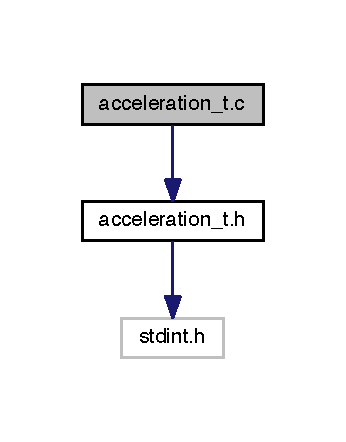
\includegraphics[width=166pt]{acceleration__t_8c__incl}
\end{center}
\end{figure}

\hypertarget{acceleration__t_8h}{\section{acceleration\-\_\-t.\-h File Reference}
\label{acceleration__t_8h}\index{acceleration\-\_\-t.\-h@{acceleration\-\_\-t.\-h}}
}
{\ttfamily \#include $<$stdint.\-h$>$}\\*
Include dependency graph for acceleration\-\_\-t.\-h\-:\nopagebreak
\begin{figure}[H]
\begin{center}
\leavevmode
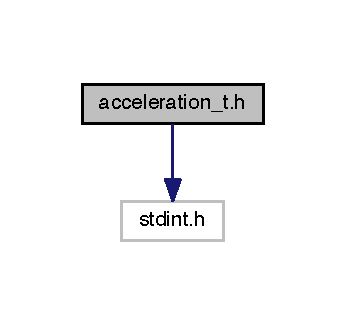
\includegraphics[width=166pt]{acceleration__t_8h__incl}
\end{center}
\end{figure}
This graph shows which files directly or indirectly include this file\-:
\nopagebreak
\begin{figure}[H]
\begin{center}
\leavevmode
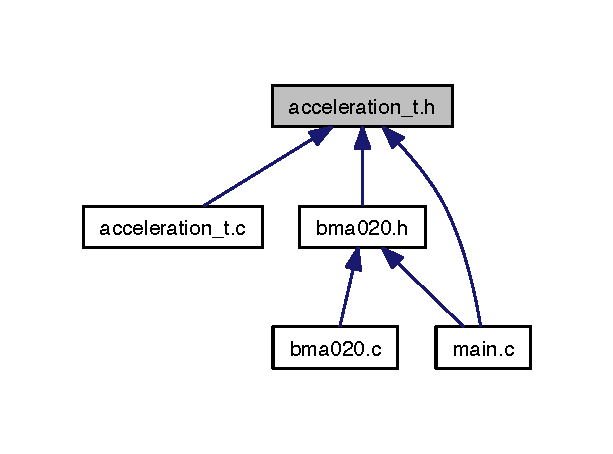
\includegraphics[width=294pt]{acceleration__t_8h__dep__incl}
\end{center}
\end{figure}
\subsection*{Data Structures}
\begin{DoxyCompactItemize}
\item 
struct \hyperlink{structacceleration__t}{acceleration\-\_\-t}
\end{DoxyCompactItemize}

\hypertarget{bma020_8c}{\section{bma020.\-c File Reference}
\label{bma020_8c}\index{bma020.\-c@{bma020.\-c}}
}
{\ttfamily \#include \char`\"{}bma020.\-h\char`\"{}}\\*
{\ttfamily \#include \char`\"{}lib/twi\-\_\-master.\-h\char`\"{}}\\*
Include dependency graph for bma020.\-c\-:
\nopagebreak
\begin{figure}[H]
\begin{center}
\leavevmode
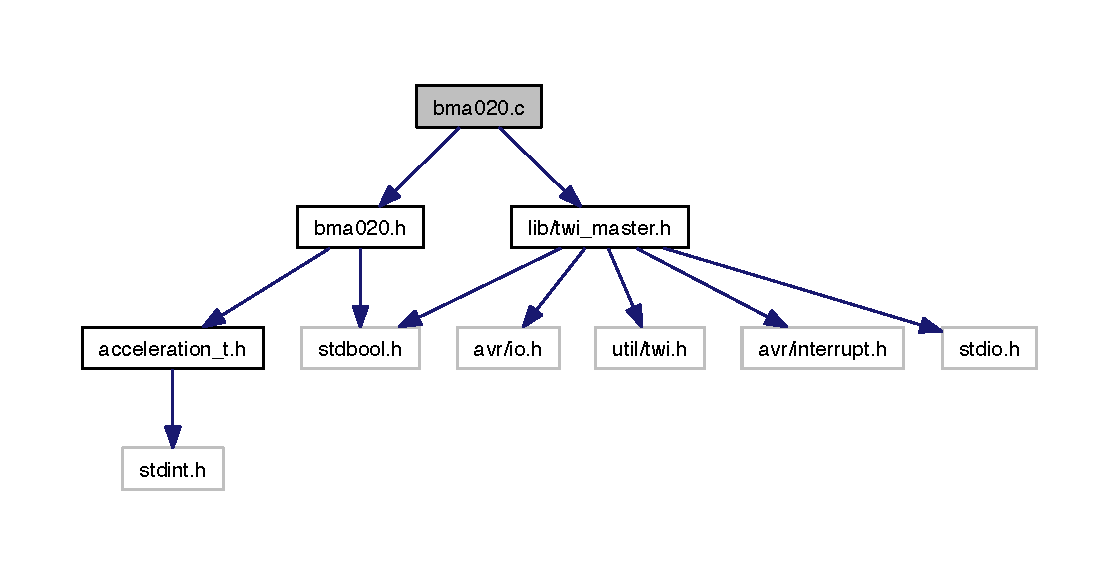
\includegraphics[width=350pt]{bma020_8c__incl}
\end{center}
\end{figure}
\subsection*{Macros}
\begin{DoxyCompactItemize}
\item 
\#define \hyperlink{bma020_8c_a910ebdcbf3fe3a5499b9d427c95369ad}{B\-M\-A020\-\_\-\-T\-W\-I\-\_\-\-A\-D\-D\-R\-E\-S\-S}~(0x70$>$$>$1)
\item 
\#define \hyperlink{bma020_8c_ae2e8a268ceac616785b0515665b01bb4}{B\-M\-A020\-\_\-\-R\-E\-G\-I\-S\-T\-E\-R\-\_\-\-C\-H\-I\-P\-I\-D}~0x00
\item 
\#define \hyperlink{bma020_8c_a36bed1b115f30a8f83929aa6912ef90f}{B\-M\-A020\-\_\-\-R\-E\-G\-I\-S\-T\-E\-R\-\_\-\-V\-E\-R\-S\-I\-O\-N}~0x01
\item 
\#define \hyperlink{bma020_8c_a6b948feae41f5da16e97ff1bd9e3334d}{B\-M\-A020\-\_\-\-R\-E\-G\-I\-S\-T\-E\-R\-\_\-\-V\-A\-L\-U\-E\-\_\-\-X\-\_\-\-L\-S\-B}~0x02
\item 
\#define \hyperlink{bma020_8c_ad3f2bc45b1d488802ca938203944ce07}{B\-M\-A020\-\_\-\-R\-E\-G\-I\-S\-T\-E\-R\-\_\-\-V\-A\-L\-U\-E\-\_\-\-X\-\_\-\-M\-S\-B}~0x03
\item 
\#define \hyperlink{bma020_8c_ac0e18c6e342e41ec51273064e789eb71}{B\-M\-A020\-\_\-\-R\-E\-G\-I\-S\-T\-E\-R\-\_\-\-V\-A\-L\-U\-E\-\_\-\-Y\-\_\-\-L\-S\-B}~0x04
\item 
\#define \hyperlink{bma020_8c_a4890cf05c47f87b1cafce312d70cbe61}{B\-M\-A020\-\_\-\-R\-E\-G\-I\-S\-T\-E\-R\-\_\-\-V\-A\-L\-U\-E\-\_\-\-Y\-\_\-\-M\-S\-B}~0x05
\item 
\#define \hyperlink{bma020_8c_a34537e4b701cf6c8ccbd35dddb50cdae}{B\-M\-A020\-\_\-\-R\-E\-G\-I\-S\-T\-E\-R\-\_\-\-V\-A\-L\-U\-E\-\_\-\-Z\-\_\-\-L\-S\-B}~0x06
\item 
\#define \hyperlink{bma020_8c_ad7d861a9c537ae4d858d675cabeb72ab}{B\-M\-A020\-\_\-\-R\-E\-G\-I\-S\-T\-E\-R\-\_\-\-V\-A\-L\-U\-E\-\_\-\-Z\-\_\-\-M\-S\-B}~0x07
\item 
\#define \hyperlink{bma020_8c_a31b18d783e0814107d12497480f83c16}{B\-M\-A020\-\_\-\-R\-E\-G\-I\-S\-T\-E\-R\-\_\-\-U\-N\-U\-S\-E\-D}~0x08
\item 
\#define \hyperlink{bma020_8c_a4b0153203b4e4eedaacb8898a981a782}{B\-M\-A020\-\_\-\-R\-E\-G\-I\-S\-T\-E\-R\-\_\-\-S\-T\-A\-T\-U\-S}~0x09
\item 
\#define \hyperlink{bma020_8c_a5e888189b9d1de2c93925224e91135ed}{B\-M\-A020\-\_\-\-R\-E\-G\-I\-S\-T\-E\-R\-\_\-\-C\-O\-N\-T\-R\-O\-L\-\_\-\-T\-E\-S\-T\-S\-\_\-\-R\-E\-S\-E\-T\-\_\-\-S\-L\-E\-E\-P}~0x0\-A
\item 
\#define \hyperlink{bma020_8c_a0d57597e9444b2d2527e51fbac95737f}{B\-M\-A020\-\_\-\-R\-E\-G\-I\-S\-T\-E\-R\-\_\-\-A\-L\-E\-R\-T\-\_\-\-E\-N\-A\-N\-Y\-M\-O\-T\-I\-O\-N\-\_\-\-C\-N\-T\-H\-G\-\_\-\-C\-N\-T\-L\-G\-\_\-\-E\-N\-H\-G\-\_\-\-E\-N\-L\-G}~0x0\-B
\item 
\#define \hyperlink{bma020_8c_a0768026989e7f0e8dafa136b0b836778}{B\-M\-A020\-\_\-\-R\-E\-G\-I\-S\-T\-E\-R\-\_\-\-L\-G\-\_\-\-T\-H\-R\-E\-S\-H\-O\-L\-D}~0x0\-C
\item 
\#define \hyperlink{bma020_8c_adb75b4cfabce54c8835a60667ca2fec6}{B\-M\-A020\-\_\-\-R\-E\-G\-I\-S\-T\-E\-R\-\_\-\-L\-G\-\_\-\-D\-U\-R\-A\-T\-I\-O\-N}~0x0\-D
\item 
\#define \hyperlink{bma020_8c_a6ae61e1f922e9dc1deac5c123c1f5392}{B\-M\-A020\-\_\-\-R\-E\-G\-I\-S\-T\-E\-R\-\_\-\-H\-G\-\_\-\-T\-H\-R\-E\-S\-H\-O\-L\-D}~0x0\-E
\item 
\#define \hyperlink{bma020_8c_a986414c08eaff36b51caf3fa4270b676}{B\-M\-A020\-\_\-\-R\-E\-G\-I\-S\-T\-E\-R\-\_\-\-H\-G\-\_\-\-D\-U\-R\-A\-T\-I\-O\-N}~0x0\-F
\item 
\#define \hyperlink{bma020_8c_a879872e3c026a4839f7a1dcce279ebbc}{B\-M\-A020\-\_\-\-R\-E\-G\-I\-S\-T\-E\-R\-\_\-\-A\-N\-Y\-\_\-\-M\-O\-T\-I\-O\-N\-\_\-\-T\-H\-R\-E\-S\-H\-O\-L\-D}~0x10
\item 
\#define \hyperlink{bma020_8c_a7948d646abd9564270e781e7d1542ea2}{B\-M\-A020\-\_\-\-R\-E\-G\-I\-S\-T\-E\-R\-\_\-\-A\-M\-D\-U\-R\-\_\-\-H\-G\-H\-Y\-S\-\_\-\-L\-G\-H\-Y\-S}~0x11
\item 
\#define \hyperlink{bma020_8c_a41a38da26d08f31a9e57b78c25c86fc3}{B\-M\-A020\-\_\-\-R\-E\-G\-I\-S\-T\-E\-R\-\_\-\-C\-U\-S\-T\-O\-M\-E\-R\-\_\-1}~0x12
\item 
\#define \hyperlink{bma020_8c_a731c45918ee8c88a458532e5aaf1e8e8}{B\-M\-A020\-\_\-\-R\-E\-G\-I\-S\-T\-E\-R\-\_\-\-C\-U\-S\-T\-O\-M\-E\-R\-\_\-2}~0x13
\item 
\#define \hyperlink{bma020_8c_a348818f726073a02dcfb2acc73b21d3c}{B\-M\-A020\-\_\-\-R\-E\-G\-I\-S\-T\-E\-R\-\_\-\-C\-O\-N\-T\-R\-O\-L\-\_\-\-R\-A\-N\-G\-E\-\_\-\-B\-A\-N\-D\-W\-I\-D\-T\-H}~0x14
\item 
\#define \hyperlink{bma020_8c_a4acb39507d72445b72e8ec37cfc7e110}{B\-M\-A020\-\_\-\-R\-E\-G\-I\-S\-T\-E\-R\-\_\-\-C\-O\-N\-T\-R\-O\-L\-\_\-\-S\-P\-I4\-\_\-\-I\-N\-T\-E\-R\-R\-U\-P\-T\-\_\-\-W\-A\-K\-E\-U\-P}~0x15
\item 
\#define \hyperlink{bma020_8c_a975fb727d6224967de9b9c59a8386b4e}{B\-M\-A020\-\_\-\-B\-I\-T\-\_\-\-S\-T\-A\-T\-U\-S\-\_\-\-H\-G}~0
\item 
\#define \hyperlink{bma020_8c_a82a0471a876781d862c73fcf2d2d294c}{B\-M\-A020\-\_\-\-B\-I\-T\-\_\-\-S\-T\-A\-T\-U\-S\-\_\-\-L\-G}~1
\item 
\#define \hyperlink{bma020_8c_ac2782347bec913ffd6b4886260d4a1c9}{B\-M\-A020\-\_\-\-B\-I\-T\-\_\-\-H\-G\-\_\-\-L\-A\-T\-C\-H\-E\-D}~2
\item 
\#define \hyperlink{bma020_8c_ac8707c5ff4823f57d53166c68b93a64d}{B\-M\-A020\-\_\-\-B\-I\-T\-\_\-\-L\-G\-\_\-\-L\-A\-T\-C\-H\-E\-D}~3
\item 
\#define \hyperlink{bma020_8c_ac632ae4a1bc7d097f799ae65f8189d8e}{B\-M\-A020\-\_\-\-B\-I\-T\-\_\-\-A\-L\-E\-R\-T\-\_\-\-P\-H\-A\-S\-E}~4
\item 
\#define \hyperlink{bma020_8c_a8cee37199daf753a3ed843455d8c2a09}{B\-M\-A020\-\_\-\-B\-I\-T\-\_\-\-S\-E\-L\-F\-\_\-\-T\-E\-S\-T\-\_\-\-R\-E\-S\-U\-L\-T}~7
\item 
\#define \hyperlink{bma020_8c_acc826408b5998aa06e5c14dff972fd6f}{B\-M\-A020\-\_\-\-B\-I\-T\-\_\-\-S\-L\-E\-E\-P}~0
\item 
\#define \hyperlink{bma020_8c_ab3a25deb0aee6d5e44900e95d425c83b}{B\-M\-A020\-\_\-\-B\-I\-T\-\_\-\-S\-O\-F\-T\-\_\-\-R\-E\-S\-E\-T}~1
\item 
\#define \hyperlink{bma020_8c_a16d0d9c77ebf3a62c7b0751085fb4d93}{B\-M\-A020\-\_\-\-B\-I\-T\-\_\-\-S\-E\-L\-F\-\_\-\-T\-E\-S\-T\-\_\-0}~2
\item 
\#define \hyperlink{bma020_8c_a7fdbfb38eda34b405088ce97d5c78c40}{B\-M\-A020\-\_\-\-B\-I\-T\-\_\-\-S\-E\-L\-F\-\_\-\-T\-E\-S\-T\-\_\-1}~3
\item 
\#define \hyperlink{bma020_8c_a165460cff50e3bf8af5fe35ffca3abc6}{B\-M\-A020\-\_\-\-B\-I\-T\-\_\-\-R\-E\-S\-E\-T\-\_\-\-I\-N\-T}~6
\item 
\#define \hyperlink{bma020_8c_a925aaafeefd3816288eb460c34837aef}{B\-M\-A020\-\_\-\-B\-I\-T\-\_\-\-E\-N\-A\-B\-L\-E\-\_\-\-L\-G}~0
\item 
\#define \hyperlink{bma020_8c_a5a3e6dcc957c52b8d335bdd974b12e94}{B\-M\-A020\-\_\-\-B\-I\-T\-\_\-\-E\-N\-A\-B\-L\-E\-\_\-\-H\-G}~1
\item 
\#define \hyperlink{bma020_8c_a6ebd350d7b315f6c7d569a78cde496ce}{B\-M\-A020\-\_\-\-B\-I\-T\-\_\-\-C\-O\-U\-N\-T\-E\-R\-\_\-\-L\-G\-\_\-0}~2
\item 
\#define \hyperlink{bma020_8c_a8538d5673ade5e44d08f5f38ee43e094}{B\-M\-A020\-\_\-\-B\-I\-T\-\_\-\-C\-O\-U\-N\-T\-E\-R\-\_\-\-L\-G\-\_\-1}~3
\item 
\#define \hyperlink{bma020_8c_a064c3ec3608ecbd1f7f379f2dd322fa7}{B\-M\-A020\-\_\-\-B\-I\-T\-\_\-\-C\-O\-U\-N\-T\-E\-R\-\_\-\-H\-G\-\_\-0}~4
\item 
\#define \hyperlink{bma020_8c_a78bb70f1295257936f12414b2581b681}{B\-M\-A020\-\_\-\-B\-I\-T\-\_\-\-C\-O\-U\-N\-T\-E\-R\-\_\-\-H\-G\-\_\-1}~5
\item 
\#define \hyperlink{bma020_8c_af7d31105bcb02dc50e6a92763a86231c}{B\-M\-A020\-\_\-\-B\-I\-T\-\_\-\-A\-N\-Y\-\_\-\-M\-O\-T\-I\-O\-N}~6
\item 
\#define \hyperlink{bma020_8c_a0a8db97d7c0230486028ca4ac0be595c}{B\-M\-A020\-\_\-\-B\-I\-T\-\_\-\-A\-L\-T\-E\-R\-T}~7
\item 
\#define \hyperlink{bma020_8c_a059560827f070835f7a4c8b313ceb84e}{B\-M\-A020\-\_\-\-B\-I\-T\-\_\-\-L\-G\-\_\-\-H\-Y\-S\-T\-E\-R\-E\-S\-I\-S\-\_\-0}~0
\item 
\#define \hyperlink{bma020_8c_a1502001a7f24242b327f1c0e47a2241c}{B\-M\-A020\-\_\-\-B\-I\-T\-\_\-\-L\-G\-\_\-\-H\-Y\-S\-T\-E\-R\-E\-S\-I\-S\-\_\-1}~1
\item 
\#define \hyperlink{bma020_8c_a576762122658d43da865ea1e86c1fc71}{B\-M\-A020\-\_\-\-B\-I\-T\-\_\-\-L\-G\-\_\-\-H\-Y\-S\-T\-E\-R\-E\-S\-I\-S\-\_\-2}~2
\item 
\#define \hyperlink{bma020_8c_a933aa5877c72d903e9ab78e9ab592cd4}{B\-M\-A020\-\_\-\-B\-I\-T\-\_\-\-H\-G\-\_\-\-H\-Y\-S\-T\-E\-R\-E\-S\-I\-S\-\_\-0}~3
\item 
\#define \hyperlink{bma020_8c_a34468ab47faece6bb997f04b7346eb87}{B\-M\-A020\-\_\-\-B\-I\-T\-\_\-\-H\-G\-\_\-\-H\-Y\-S\-T\-E\-R\-E\-S\-I\-S\-\_\-1}~4
\item 
\#define \hyperlink{bma020_8c_a19d394a2a00ac726548dae99f86eabd1}{B\-M\-A020\-\_\-\-B\-I\-T\-\_\-\-H\-G\-\_\-\-H\-Y\-S\-T\-E\-R\-E\-S\-I\-S\-\_\-2}~5
\item 
\#define \hyperlink{bma020_8c_abbb0a86052c45170a3d6bec56231b6d1}{B\-M\-A020\-\_\-\-B\-I\-T\-\_\-\-A\-N\-Y\-\_\-\-M\-O\-T\-I\-O\-N\-\_\-\-D\-U\-R\-A\-T\-I\-O\-N\-\_\-0}~6
\item 
\#define \hyperlink{bma020_8c_a236cae0610d4977b7c33d61da6c0283a}{B\-M\-A020\-\_\-\-B\-I\-T\-\_\-\-A\-N\-Y\-\_\-\-M\-O\-T\-I\-O\-N\-\_\-\-D\-U\-R\-A\-T\-I\-O\-N\-\_\-1}~7
\item 
\#define \hyperlink{bma020_8c_aa800c186a424bd30d9a74171485a6637}{B\-M\-A020\-\_\-\-B\-I\-T\-\_\-\-B\-A\-N\-D\-W\-I\-D\-T\-H\-\_\-0}~0
\item 
\#define \hyperlink{bma020_8c_a1988901e033e97c59ecf3a7838105965}{B\-M\-A020\-\_\-\-B\-I\-T\-\_\-\-B\-A\-N\-D\-W\-I\-D\-T\-H\-\_\-1}~1
\item 
\#define \hyperlink{bma020_8c_a544b437e7c147c78f0d5c7809aa30ef4}{B\-M\-A020\-\_\-\-B\-I\-T\-\_\-\-B\-A\-N\-D\-W\-I\-D\-T\-H\-\_\-2}~2
\item 
\#define \hyperlink{bma020_8c_a50cb14ce8207239ab2c36e499a9cd70f}{B\-M\-A020\-\_\-\-B\-I\-T\-\_\-\-R\-A\-N\-G\-E\-\_\-0}~3
\item 
\#define \hyperlink{bma020_8c_a0c818caa68bb04f65df611469144ae24}{B\-M\-A020\-\_\-\-B\-I\-T\-\_\-\-R\-A\-N\-G\-E\-\_\-1}~4
\item 
\#define \hyperlink{bma020_8c_aa805f5b363f2c391346bfc3d320a025d}{B\-M\-A020\-\_\-\-B\-I\-T\-\_\-\-W\-A\-K\-E\-\_\-\-U\-P}~0
\item 
\#define \hyperlink{bma020_8c_a689c1751e1bca1798ebe5475811a0fcb}{B\-M\-A020\-\_\-\-B\-I\-T\-\_\-\-W\-A\-K\-E\-\_\-\-U\-P\-\_\-\-P\-A\-U\-S\-E\-\_\-0}~1
\item 
\#define \hyperlink{bma020_8c_ae682be14fa6f0456267646dbf61663e2}{B\-M\-A020\-\_\-\-B\-I\-T\-\_\-\-W\-A\-K\-E\-\_\-\-U\-P\-\_\-\-P\-A\-U\-S\-E\-\_\-1}~2
\item 
\#define \hyperlink{bma020_8c_ab60ba5f17308fb2482b5a2c612c42a8b}{B\-M\-A020\-\_\-\-B\-I\-T\-\_\-\-S\-H\-A\-D\-O\-W\-\_\-\-D\-I\-S}~3
\item 
\#define \hyperlink{bma020_8c_ad5d46d9c4eb32f7bb2c583852a762f86}{B\-M\-A020\-\_\-\-B\-I\-T\-\_\-\-L\-A\-T\-C\-H\-\_\-\-I\-N\-T}~4
\item 
\#define \hyperlink{bma020_8c_aff110e4eec403c02f3bb802db28b56e3}{B\-M\-A020\-\_\-\-B\-I\-T\-\_\-\-N\-E\-W\-\_\-\-D\-A\-T\-A\-\_\-\-I\-N\-T}~5
\item 
\#define \hyperlink{bma020_8c_a86fd77658f1cd3d91f7a0b4ceef55d1b}{B\-M\-A020\-\_\-\-B\-I\-T\-\_\-\-A\-D\-V\-A\-N\-C\-E\-D\-\_\-\-I\-N\-T}~6
\item 
\#define \hyperlink{bma020_8c_a8100c404a0fb79baa3a2f9540223e01b}{B\-M\-A020\-\_\-\-B\-I\-T\-\_\-\-S\-P\-I4}~7
\end{DoxyCompactItemize}
\subsection*{Functions}
\begin{DoxyCompactItemize}
\item 
uint8\-\_\-t \hyperlink{bma020_8c_af61528e1bbdc91a9acac39c776cfc11b}{bma020\-\_\-get\-\_\-chip\-\_\-id} ()
\item 
uint8\-\_\-t \hyperlink{bma020_8c_ad815b4dc0e95fa9e9109930e4c1ba39a}{bma020\-\_\-get\-\_\-ml\-\_\-version} ()
\item 
uint8\-\_\-t \hyperlink{bma020_8c_a411ed87bf0eebcd6464a2efa0b303940}{bma020\-\_\-get\-\_\-ai\-\_\-version} ()
\item 
void \hyperlink{bma020_8c_a26f79cde9e7a22ae5727f39850fc5eae}{bma020\-\_\-read\-\_\-raw\-\_\-acceleration} (\hyperlink{structacceleration__t}{acceleration\-\_\-t} $\ast$raw\-\_\-a\-\_\-vector)
\item 
bool \hyperlink{bma020_8c_aa3922b9a261401e957502b0dc0c5395a}{bma020\-\_\-is\-\_\-new\-\_\-data} (char axis)
\item 
bool \hyperlink{bma020_8c_af8352dba63a90d34734410f4f97eced4}{bma020\-\_\-get\-\_\-status\-\_\-hg} (void)
\item 
bool \hyperlink{bma020_8c_ab06787c50f090a339e8ed4d4a1408f6b}{bma020\-\_\-get\-\_\-status\-\_\-lg} (void)
\item 
bool \hyperlink{bma020_8c_a48178f75ec28ec3a881c0bd23ec16dfc}{bma020\-\_\-get\-\_\-lg\-\_\-latched} (void)
\item 
void \hyperlink{bma020_8c_aa591678c9c225c04379f31f443da516f}{bma020\-\_\-reset\-\_\-lg\-\_\-latched} (void)
\item 
bool \hyperlink{bma020_8c_a5607b1f4a151f90262f63ac79ec8dbd9}{bma020\-\_\-get\-\_\-hg\-\_\-latched} (void)
\item 
void \hyperlink{bma020_8c_a996664698b38ebcbdc5f35277c86271f}{bma020\-\_\-reset\-\_\-hg\-\_\-latched} (void)
\item 
bool \hyperlink{bma020_8c_ada7359286e7b2e8f5efe66dbc7e0ec3e}{bma020\-\_\-get\-\_\-alert\-\_\-phase} (void)
\item 
bool \hyperlink{bma020_8c_a225a6d888c491bc9eeaa587c71658530}{bma020\-\_\-get\-\_\-self\-\_\-test\-\_\-result} (void)
\item 
void \hyperlink{bma020_8c_ae46fb2b7063713e26d4f939a01c410b4}{bma020\-\_\-sleep} (void)
\item 
void \hyperlink{bma020_8c_aee5899ae2a2762d1f20c4f2895298e34}{bma020\-\_\-soft\-\_\-reset} (void)
\item 
void \hyperlink{bma020_8c_a1b4d80e962496fd3d254dc1adb060ccd}{bma020\-\_\-perform\-\_\-self\-\_\-test\-\_\-0} (void)
\item 
void \hyperlink{bma020_8c_aafad8d4b857d14f771e1b5584b540087}{bma020\-\_\-perform\-\_\-self\-\_\-test\-\_\-1} (void)
\item 
void \hyperlink{bma020_8c_a81d4cd9fa30f06a446febbde9b62cef1}{bma020\-\_\-enable\-\_\-spi4} (bool enable)
\item 
bool \hyperlink{bma020_8c_a62a15f74e49f2463c1872dbe43dce521}{bma020\-\_\-is\-\_\-spi4} (void)
\item 
void \hyperlink{bma020_8c_a074b9f65e1bfa1b5bb770e465275a780}{bma020\-\_\-disable\-\_\-shadow} (bool disable)
\item 
bool \hyperlink{bma020_8c_ad5d778ebe7f19ffc5447b05392bc81d5}{bma020\-\_\-is\-\_\-shadow\-\_\-disabled} (void)
\item 
void \hyperlink{bma020_8c_ac523767751ba8462faae363f828af936}{bma020\-\_\-reset\-\_\-interrupt} (void)
\item 
void \hyperlink{bma020_8c_aeec5f00abc70a8693a10b23f12e25ab6}{bma020\-\_\-enable\-\_\-new\-\_\-data\-\_\-int} (bool enable)
\item 
bool \hyperlink{bma020_8c_a3f70726f60c671a6cd7250c84cc9ee7a}{bma020\-\_\-is\-\_\-new\-\_\-data\-\_\-int} (void)
\item 
void \hyperlink{bma020_8c_a8e25a2cb420e06ca77ea5b0d97c32e82}{bma020\-\_\-enable\-\_\-lg} (bool enable)
\item 
bool \hyperlink{bma020_8c_a47004eaf6774aa870fd8e2d4d5c1ae80}{bma020\-\_\-is\-\_\-enable\-\_\-lg} (void)
\item 
void \hyperlink{bma020_8c_ac3fa540d0f8c03f95efc25d8798f42b6}{bma020\-\_\-enable\-\_\-hg} (bool enable)
\item 
bool \hyperlink{bma020_8c_a8bbc44dd5bf3320c9ea06ce54100fafc}{bma020\-\_\-is\-\_\-enable\-\_\-hg} (void)
\item 
void \hyperlink{bma020_8c_aeb518ad22636eeb17dd1113306c17e1e}{bma020\-\_\-enable\-\_\-advanced\-\_\-int} (bool enable)
\item 
bool \hyperlink{bma020_8c_a7d48379dad99c291f448af6889a10c65}{bma020\-\_\-is\-\_\-advanced\-\_\-int} (void)
\item 
void \hyperlink{bma020_8c_ae69d8ecda7ddd2b067989f4a78718969}{bma020\-\_\-enable\-\_\-any\-\_\-motion} (bool enable)
\item 
bool \hyperlink{bma020_8c_a7aaedcf13c31ab032c6014cf2f11d03e}{bma020\-\_\-is\-\_\-enable\-\_\-any\-\_\-motion} (void)
\item 
void \hyperlink{bma020_8c_a9ae38bcf7e1bbb2a12b62b8d1dc3d8e2}{bma020\-\_\-enable\-\_\-motion\-\_\-alert} (bool enable)
\item 
bool \hyperlink{bma020_8c_a460b42665cb432f91a3e54c132f9891e}{bma020\-\_\-is\-\_\-enable\-\_\-motion\-\_\-alert} (void)
\item 
void \hyperlink{bma020_8c_a9e25d8b9f372bf654a72ed94dd5b4a74}{bma020\-\_\-enable\-\_\-latched\-\_\-int} (bool enable)
\item 
bool \hyperlink{bma020_8c_a3e5636663c087915feeacb349b44ce31}{bma020\-\_\-is\-\_\-latched\-\_\-int} (void)
\item 
void \hyperlink{bma020_8c_ab3fa54af803bedc74927f8f2cf00aedc}{bma020\-\_\-set\-\_\-lg\-\_\-threshold} (uint8\-\_\-t threshold)
\item 
uint8\-\_\-t \hyperlink{bma020_8c_ab9c52c7427ba44b7f40c7de7effd6b70}{bma020\-\_\-get\-\_\-lg\-\_\-threshold} ()
\item 
void \hyperlink{bma020_8c_a76e0c3a6398d21ff31571d06dff824a8}{bma020\-\_\-set\-\_\-lg\-\_\-duration} (uint8\-\_\-t duration)
\item 
uint8\-\_\-t \hyperlink{bma020_8c_af3021e4c25165a76c664be19c968ed7a}{bma020\-\_\-get\-\_\-lg\-\_\-duration} ()
\item 
bool \hyperlink{bma020_8c_a60af41cd9745b579ec231ecbcc61868e}{bma020\-\_\-set\-\_\-counter\-\_\-lg} (uint8\-\_\-t counter)
\item 
uint8\-\_\-t \hyperlink{bma020_8c_a851c0bbf26d7d95e294beae813e2c6f8}{bma020\-\_\-get\-\_\-counter\-\_\-lg} (void)
\item 
void \hyperlink{bma020_8c_acf15f8f2a17ea937719f4f49af0c019f}{bma020\-\_\-set\-\_\-lg\-\_\-hysterese} (uint8\-\_\-t hysterese)
\item 
uint8\-\_\-t \hyperlink{bma020_8c_a73397e5a2d7ec9443c34e9f2fd4e7e8e}{bma020\-\_\-get\-\_\-lg\-\_\-hysterese} (void)
\item 
void \hyperlink{bma020_8c_aae208059c28e62103471091593e14777}{bma020\-\_\-set\-\_\-hg\-\_\-threshold} (uint8\-\_\-t threshold)
\item 
uint8\-\_\-t \hyperlink{bma020_8c_a7574ff05e7bc504eb37df267bd1a6d54}{bma020\-\_\-get\-\_\-hg\-\_\-threshold} ()
\item 
void \hyperlink{bma020_8c_a285be18086194248979609a9333e0a47}{bma020\-\_\-set\-\_\-hg\-\_\-duration} (uint8\-\_\-t duration)
\item 
uint8\-\_\-t \hyperlink{bma020_8c_a298d59459d1e3fd4a27ad187027ecea2}{bma020\-\_\-get\-\_\-hg\-\_\-duration} ()
\item 
bool \hyperlink{bma020_8c_ad8ef8d59af38fd4b7a2e271a433eb36a}{bma020\-\_\-set\-\_\-counter\-\_\-hg} (uint8\-\_\-t counter)
\item 
uint8\-\_\-t \hyperlink{bma020_8c_aec5666921548a0d1a7c81c9b71dd9d44}{bma020\-\_\-get\-\_\-counter\-\_\-hg} (void)
\item 
void \hyperlink{bma020_8c_a918407085e71e3ceb626d46afb0f36e0}{bma020\-\_\-set\-\_\-hg\-\_\-hysterese} (uint8\-\_\-t hysterese)
\item 
uint8\-\_\-t \hyperlink{bma020_8c_a532014744107ba2e88a56d2c4119db40}{bma020\-\_\-get\-\_\-hg\-\_\-hysterese} (void)
\item 
void \hyperlink{bma020_8c_ab98b298250deca2b3e71ac59d9f8ddd3}{bma020\-\_\-set\-\_\-any\-\_\-motion\-\_\-threshold} (uint8\-\_\-t threshold)
\item 
uint8\-\_\-t \hyperlink{bma020_8c_aa886f09ffd7a8a7237198a56ee262fc5}{bma020\-\_\-get\-\_\-any\-\_\-motion\-\_\-threshold} (void)
\item 
bool \hyperlink{bma020_8c_a487a45e193399a5d13f378b130989447}{bma020\-\_\-set\-\_\-any\-\_\-motion\-\_\-duration} (uint8\-\_\-t duration)
\item 
uint8\-\_\-t \hyperlink{bma020_8c_aa0957d9a759593bf02c37f61dac4a41b}{bma020\-\_\-get\-\_\-any\-\_\-motion\-\_\-duration} (void)
\item 
void \hyperlink{bma020_8c_a84ad4c88f3a38ec91b3639e58ded55ae}{bma020\-\_\-enable\-\_\-wake\-\_\-up} (bool enable)
\item 
bool \hyperlink{bma020_8c_a754386a5ed68093f02f5bec3f5e98cbd}{bma020\-\_\-is\-\_\-wake\-\_\-up} (void)
\item 
bool \hyperlink{bma020_8c_ae73261ee46188952993f69970854e386}{bma020\-\_\-set\-\_\-wake\-\_\-up\-\_\-pause} (uint16\-\_\-t wake\-\_\-up\-\_\-time)
\item 
uint16\-\_\-t \hyperlink{bma020_8c_a9e076fdb4daec0fe8352340385006b7d}{bma020\-\_\-get\-\_\-wake\-\_\-up\-\_\-pause} (void)
\item 
bool \hyperlink{bma020_8c_a4c14ca5b6efeec9be6739252812ba8ae}{bma020\-\_\-set\-\_\-bandwidth} (uint16\-\_\-t bandwidth)
\item 
uint16\-\_\-t \hyperlink{bma020_8c_a7638286b73693422b67c4fabef32fe24}{bma020\-\_\-get\-\_\-bandwidth} (void)
\item 
bool \hyperlink{bma020_8c_a503460a9fa8d3366a3fd57bc3e278c5c}{bma020\-\_\-set\-\_\-range} (uint8\-\_\-t range)
\item 
uint8\-\_\-t \hyperlink{bma020_8c_a9a0c0e161ae1c7ac0963a98f1a499c00}{bma020\-\_\-get\-\_\-range} (void)
\item 
void \hyperlink{bma020_8c_af0a438e715f02efa689bc251ccbb8050}{bma020\-\_\-set\-\_\-customer\-\_\-reserved\-\_\-1} (uint8\-\_\-t value)
\item 
uint8\-\_\-t \hyperlink{bma020_8c_a772e31e89870de0eebfdf2d00bbf145a}{bma020\-\_\-get\-\_\-customer\-\_\-reserved\-\_\-1} ()
\item 
void \hyperlink{bma020_8c_aff774b72ecf7cfae5dd7855cac989953}{bma020\-\_\-set\-\_\-customer\-\_\-reserved\-\_\-2} (uint8\-\_\-t value)
\item 
uint8\-\_\-t \hyperlink{bma020_8c_a57c220a687c54813b3971dbb53e4d341}{bma020\-\_\-get\-\_\-customer\-\_\-reserved\-\_\-2} ()
\item 
void \hyperlink{bma020_8c_ac5c1a01ed031d3c8826f4a54cbae6efe}{bma020\-\_\-init} (void)
\end{DoxyCompactItemize}


\subsection{Macro Definition Documentation}
\hypertarget{bma020_8c_a86fd77658f1cd3d91f7a0b4ceef55d1b}{\index{bma020.\-c@{bma020.\-c}!B\-M\-A020\-\_\-\-B\-I\-T\-\_\-\-A\-D\-V\-A\-N\-C\-E\-D\-\_\-\-I\-N\-T@{B\-M\-A020\-\_\-\-B\-I\-T\-\_\-\-A\-D\-V\-A\-N\-C\-E\-D\-\_\-\-I\-N\-T}}
\index{B\-M\-A020\-\_\-\-B\-I\-T\-\_\-\-A\-D\-V\-A\-N\-C\-E\-D\-\_\-\-I\-N\-T@{B\-M\-A020\-\_\-\-B\-I\-T\-\_\-\-A\-D\-V\-A\-N\-C\-E\-D\-\_\-\-I\-N\-T}!bma020.c@{bma020.\-c}}
\subsubsection[{B\-M\-A020\-\_\-\-B\-I\-T\-\_\-\-A\-D\-V\-A\-N\-C\-E\-D\-\_\-\-I\-N\-T}]{\setlength{\rightskip}{0pt plus 5cm}\#define B\-M\-A020\-\_\-\-B\-I\-T\-\_\-\-A\-D\-V\-A\-N\-C\-E\-D\-\_\-\-I\-N\-T~6}}\label{bma020_8c_a86fd77658f1cd3d91f7a0b4ceef55d1b}


Definition at line 94 of file bma020.\-c.



Referenced by bma020\-\_\-enable\-\_\-advanced\-\_\-int(), and bma020\-\_\-is\-\_\-advanced\-\_\-int().

\hypertarget{bma020_8c_ac632ae4a1bc7d097f799ae65f8189d8e}{\index{bma020.\-c@{bma020.\-c}!B\-M\-A020\-\_\-\-B\-I\-T\-\_\-\-A\-L\-E\-R\-T\-\_\-\-P\-H\-A\-S\-E@{B\-M\-A020\-\_\-\-B\-I\-T\-\_\-\-A\-L\-E\-R\-T\-\_\-\-P\-H\-A\-S\-E}}
\index{B\-M\-A020\-\_\-\-B\-I\-T\-\_\-\-A\-L\-E\-R\-T\-\_\-\-P\-H\-A\-S\-E@{B\-M\-A020\-\_\-\-B\-I\-T\-\_\-\-A\-L\-E\-R\-T\-\_\-\-P\-H\-A\-S\-E}!bma020.c@{bma020.\-c}}
\subsubsection[{B\-M\-A020\-\_\-\-B\-I\-T\-\_\-\-A\-L\-E\-R\-T\-\_\-\-P\-H\-A\-S\-E}]{\setlength{\rightskip}{0pt plus 5cm}\#define B\-M\-A020\-\_\-\-B\-I\-T\-\_\-\-A\-L\-E\-R\-T\-\_\-\-P\-H\-A\-S\-E~4}}\label{bma020_8c_ac632ae4a1bc7d097f799ae65f8189d8e}


Definition at line 50 of file bma020.\-c.



Referenced by bma020\-\_\-get\-\_\-alert\-\_\-phase().

\hypertarget{bma020_8c_a0a8db97d7c0230486028ca4ac0be595c}{\index{bma020.\-c@{bma020.\-c}!B\-M\-A020\-\_\-\-B\-I\-T\-\_\-\-A\-L\-T\-E\-R\-T@{B\-M\-A020\-\_\-\-B\-I\-T\-\_\-\-A\-L\-T\-E\-R\-T}}
\index{B\-M\-A020\-\_\-\-B\-I\-T\-\_\-\-A\-L\-T\-E\-R\-T@{B\-M\-A020\-\_\-\-B\-I\-T\-\_\-\-A\-L\-T\-E\-R\-T}!bma020.c@{bma020.\-c}}
\subsubsection[{B\-M\-A020\-\_\-\-B\-I\-T\-\_\-\-A\-L\-T\-E\-R\-T}]{\setlength{\rightskip}{0pt plus 5cm}\#define B\-M\-A020\-\_\-\-B\-I\-T\-\_\-\-A\-L\-T\-E\-R\-T~7}}\label{bma020_8c_a0a8db97d7c0230486028ca4ac0be595c}


Definition at line 68 of file bma020.\-c.



Referenced by bma020\-\_\-enable\-\_\-motion\-\_\-alert(), and bma020\-\_\-is\-\_\-enable\-\_\-motion\-\_\-alert().

\hypertarget{bma020_8c_af7d31105bcb02dc50e6a92763a86231c}{\index{bma020.\-c@{bma020.\-c}!B\-M\-A020\-\_\-\-B\-I\-T\-\_\-\-A\-N\-Y\-\_\-\-M\-O\-T\-I\-O\-N@{B\-M\-A020\-\_\-\-B\-I\-T\-\_\-\-A\-N\-Y\-\_\-\-M\-O\-T\-I\-O\-N}}
\index{B\-M\-A020\-\_\-\-B\-I\-T\-\_\-\-A\-N\-Y\-\_\-\-M\-O\-T\-I\-O\-N@{B\-M\-A020\-\_\-\-B\-I\-T\-\_\-\-A\-N\-Y\-\_\-\-M\-O\-T\-I\-O\-N}!bma020.c@{bma020.\-c}}
\subsubsection[{B\-M\-A020\-\_\-\-B\-I\-T\-\_\-\-A\-N\-Y\-\_\-\-M\-O\-T\-I\-O\-N}]{\setlength{\rightskip}{0pt plus 5cm}\#define B\-M\-A020\-\_\-\-B\-I\-T\-\_\-\-A\-N\-Y\-\_\-\-M\-O\-T\-I\-O\-N~6}}\label{bma020_8c_af7d31105bcb02dc50e6a92763a86231c}


Definition at line 67 of file bma020.\-c.



Referenced by bma020\-\_\-enable\-\_\-any\-\_\-motion(), and bma020\-\_\-is\-\_\-enable\-\_\-any\-\_\-motion().

\hypertarget{bma020_8c_abbb0a86052c45170a3d6bec56231b6d1}{\index{bma020.\-c@{bma020.\-c}!B\-M\-A020\-\_\-\-B\-I\-T\-\_\-\-A\-N\-Y\-\_\-\-M\-O\-T\-I\-O\-N\-\_\-\-D\-U\-R\-A\-T\-I\-O\-N\-\_\-0@{B\-M\-A020\-\_\-\-B\-I\-T\-\_\-\-A\-N\-Y\-\_\-\-M\-O\-T\-I\-O\-N\-\_\-\-D\-U\-R\-A\-T\-I\-O\-N\-\_\-0}}
\index{B\-M\-A020\-\_\-\-B\-I\-T\-\_\-\-A\-N\-Y\-\_\-\-M\-O\-T\-I\-O\-N\-\_\-\-D\-U\-R\-A\-T\-I\-O\-N\-\_\-0@{B\-M\-A020\-\_\-\-B\-I\-T\-\_\-\-A\-N\-Y\-\_\-\-M\-O\-T\-I\-O\-N\-\_\-\-D\-U\-R\-A\-T\-I\-O\-N\-\_\-0}!bma020.c@{bma020.\-c}}
\subsubsection[{B\-M\-A020\-\_\-\-B\-I\-T\-\_\-\-A\-N\-Y\-\_\-\-M\-O\-T\-I\-O\-N\-\_\-\-D\-U\-R\-A\-T\-I\-O\-N\-\_\-0}]{\setlength{\rightskip}{0pt plus 5cm}\#define B\-M\-A020\-\_\-\-B\-I\-T\-\_\-\-A\-N\-Y\-\_\-\-M\-O\-T\-I\-O\-N\-\_\-\-D\-U\-R\-A\-T\-I\-O\-N\-\_\-0~6}}\label{bma020_8c_abbb0a86052c45170a3d6bec56231b6d1}


Definition at line 77 of file bma020.\-c.



Referenced by bma020\-\_\-get\-\_\-any\-\_\-motion\-\_\-duration(), and bma020\-\_\-set\-\_\-any\-\_\-motion\-\_\-duration().

\hypertarget{bma020_8c_a236cae0610d4977b7c33d61da6c0283a}{\index{bma020.\-c@{bma020.\-c}!B\-M\-A020\-\_\-\-B\-I\-T\-\_\-\-A\-N\-Y\-\_\-\-M\-O\-T\-I\-O\-N\-\_\-\-D\-U\-R\-A\-T\-I\-O\-N\-\_\-1@{B\-M\-A020\-\_\-\-B\-I\-T\-\_\-\-A\-N\-Y\-\_\-\-M\-O\-T\-I\-O\-N\-\_\-\-D\-U\-R\-A\-T\-I\-O\-N\-\_\-1}}
\index{B\-M\-A020\-\_\-\-B\-I\-T\-\_\-\-A\-N\-Y\-\_\-\-M\-O\-T\-I\-O\-N\-\_\-\-D\-U\-R\-A\-T\-I\-O\-N\-\_\-1@{B\-M\-A020\-\_\-\-B\-I\-T\-\_\-\-A\-N\-Y\-\_\-\-M\-O\-T\-I\-O\-N\-\_\-\-D\-U\-R\-A\-T\-I\-O\-N\-\_\-1}!bma020.c@{bma020.\-c}}
\subsubsection[{B\-M\-A020\-\_\-\-B\-I\-T\-\_\-\-A\-N\-Y\-\_\-\-M\-O\-T\-I\-O\-N\-\_\-\-D\-U\-R\-A\-T\-I\-O\-N\-\_\-1}]{\setlength{\rightskip}{0pt plus 5cm}\#define B\-M\-A020\-\_\-\-B\-I\-T\-\_\-\-A\-N\-Y\-\_\-\-M\-O\-T\-I\-O\-N\-\_\-\-D\-U\-R\-A\-T\-I\-O\-N\-\_\-1~7}}\label{bma020_8c_a236cae0610d4977b7c33d61da6c0283a}


Definition at line 78 of file bma020.\-c.



Referenced by bma020\-\_\-get\-\_\-any\-\_\-motion\-\_\-duration(), and bma020\-\_\-set\-\_\-any\-\_\-motion\-\_\-duration().

\hypertarget{bma020_8c_aa800c186a424bd30d9a74171485a6637}{\index{bma020.\-c@{bma020.\-c}!B\-M\-A020\-\_\-\-B\-I\-T\-\_\-\-B\-A\-N\-D\-W\-I\-D\-T\-H\-\_\-0@{B\-M\-A020\-\_\-\-B\-I\-T\-\_\-\-B\-A\-N\-D\-W\-I\-D\-T\-H\-\_\-0}}
\index{B\-M\-A020\-\_\-\-B\-I\-T\-\_\-\-B\-A\-N\-D\-W\-I\-D\-T\-H\-\_\-0@{B\-M\-A020\-\_\-\-B\-I\-T\-\_\-\-B\-A\-N\-D\-W\-I\-D\-T\-H\-\_\-0}!bma020.c@{bma020.\-c}}
\subsubsection[{B\-M\-A020\-\_\-\-B\-I\-T\-\_\-\-B\-A\-N\-D\-W\-I\-D\-T\-H\-\_\-0}]{\setlength{\rightskip}{0pt plus 5cm}\#define B\-M\-A020\-\_\-\-B\-I\-T\-\_\-\-B\-A\-N\-D\-W\-I\-D\-T\-H\-\_\-0~0}}\label{bma020_8c_aa800c186a424bd30d9a74171485a6637}


Definition at line 81 of file bma020.\-c.



Referenced by bma020\-\_\-get\-\_\-bandwidth(), and bma020\-\_\-set\-\_\-bandwidth().

\hypertarget{bma020_8c_a1988901e033e97c59ecf3a7838105965}{\index{bma020.\-c@{bma020.\-c}!B\-M\-A020\-\_\-\-B\-I\-T\-\_\-\-B\-A\-N\-D\-W\-I\-D\-T\-H\-\_\-1@{B\-M\-A020\-\_\-\-B\-I\-T\-\_\-\-B\-A\-N\-D\-W\-I\-D\-T\-H\-\_\-1}}
\index{B\-M\-A020\-\_\-\-B\-I\-T\-\_\-\-B\-A\-N\-D\-W\-I\-D\-T\-H\-\_\-1@{B\-M\-A020\-\_\-\-B\-I\-T\-\_\-\-B\-A\-N\-D\-W\-I\-D\-T\-H\-\_\-1}!bma020.c@{bma020.\-c}}
\subsubsection[{B\-M\-A020\-\_\-\-B\-I\-T\-\_\-\-B\-A\-N\-D\-W\-I\-D\-T\-H\-\_\-1}]{\setlength{\rightskip}{0pt plus 5cm}\#define B\-M\-A020\-\_\-\-B\-I\-T\-\_\-\-B\-A\-N\-D\-W\-I\-D\-T\-H\-\_\-1~1}}\label{bma020_8c_a1988901e033e97c59ecf3a7838105965}


Definition at line 82 of file bma020.\-c.



Referenced by bma020\-\_\-get\-\_\-bandwidth(), and bma020\-\_\-set\-\_\-bandwidth().

\hypertarget{bma020_8c_a544b437e7c147c78f0d5c7809aa30ef4}{\index{bma020.\-c@{bma020.\-c}!B\-M\-A020\-\_\-\-B\-I\-T\-\_\-\-B\-A\-N\-D\-W\-I\-D\-T\-H\-\_\-2@{B\-M\-A020\-\_\-\-B\-I\-T\-\_\-\-B\-A\-N\-D\-W\-I\-D\-T\-H\-\_\-2}}
\index{B\-M\-A020\-\_\-\-B\-I\-T\-\_\-\-B\-A\-N\-D\-W\-I\-D\-T\-H\-\_\-2@{B\-M\-A020\-\_\-\-B\-I\-T\-\_\-\-B\-A\-N\-D\-W\-I\-D\-T\-H\-\_\-2}!bma020.c@{bma020.\-c}}
\subsubsection[{B\-M\-A020\-\_\-\-B\-I\-T\-\_\-\-B\-A\-N\-D\-W\-I\-D\-T\-H\-\_\-2}]{\setlength{\rightskip}{0pt plus 5cm}\#define B\-M\-A020\-\_\-\-B\-I\-T\-\_\-\-B\-A\-N\-D\-W\-I\-D\-T\-H\-\_\-2~2}}\label{bma020_8c_a544b437e7c147c78f0d5c7809aa30ef4}


Definition at line 83 of file bma020.\-c.



Referenced by bma020\-\_\-get\-\_\-bandwidth(), and bma020\-\_\-set\-\_\-bandwidth().

\hypertarget{bma020_8c_a064c3ec3608ecbd1f7f379f2dd322fa7}{\index{bma020.\-c@{bma020.\-c}!B\-M\-A020\-\_\-\-B\-I\-T\-\_\-\-C\-O\-U\-N\-T\-E\-R\-\_\-\-H\-G\-\_\-0@{B\-M\-A020\-\_\-\-B\-I\-T\-\_\-\-C\-O\-U\-N\-T\-E\-R\-\_\-\-H\-G\-\_\-0}}
\index{B\-M\-A020\-\_\-\-B\-I\-T\-\_\-\-C\-O\-U\-N\-T\-E\-R\-\_\-\-H\-G\-\_\-0@{B\-M\-A020\-\_\-\-B\-I\-T\-\_\-\-C\-O\-U\-N\-T\-E\-R\-\_\-\-H\-G\-\_\-0}!bma020.c@{bma020.\-c}}
\subsubsection[{B\-M\-A020\-\_\-\-B\-I\-T\-\_\-\-C\-O\-U\-N\-T\-E\-R\-\_\-\-H\-G\-\_\-0}]{\setlength{\rightskip}{0pt plus 5cm}\#define B\-M\-A020\-\_\-\-B\-I\-T\-\_\-\-C\-O\-U\-N\-T\-E\-R\-\_\-\-H\-G\-\_\-0~4}}\label{bma020_8c_a064c3ec3608ecbd1f7f379f2dd322fa7}


Definition at line 65 of file bma020.\-c.



Referenced by bma020\-\_\-get\-\_\-counter\-\_\-hg(), and bma020\-\_\-set\-\_\-counter\-\_\-hg().

\hypertarget{bma020_8c_a78bb70f1295257936f12414b2581b681}{\index{bma020.\-c@{bma020.\-c}!B\-M\-A020\-\_\-\-B\-I\-T\-\_\-\-C\-O\-U\-N\-T\-E\-R\-\_\-\-H\-G\-\_\-1@{B\-M\-A020\-\_\-\-B\-I\-T\-\_\-\-C\-O\-U\-N\-T\-E\-R\-\_\-\-H\-G\-\_\-1}}
\index{B\-M\-A020\-\_\-\-B\-I\-T\-\_\-\-C\-O\-U\-N\-T\-E\-R\-\_\-\-H\-G\-\_\-1@{B\-M\-A020\-\_\-\-B\-I\-T\-\_\-\-C\-O\-U\-N\-T\-E\-R\-\_\-\-H\-G\-\_\-1}!bma020.c@{bma020.\-c}}
\subsubsection[{B\-M\-A020\-\_\-\-B\-I\-T\-\_\-\-C\-O\-U\-N\-T\-E\-R\-\_\-\-H\-G\-\_\-1}]{\setlength{\rightskip}{0pt plus 5cm}\#define B\-M\-A020\-\_\-\-B\-I\-T\-\_\-\-C\-O\-U\-N\-T\-E\-R\-\_\-\-H\-G\-\_\-1~5}}\label{bma020_8c_a78bb70f1295257936f12414b2581b681}


Definition at line 66 of file bma020.\-c.



Referenced by bma020\-\_\-get\-\_\-counter\-\_\-hg(), and bma020\-\_\-set\-\_\-counter\-\_\-hg().

\hypertarget{bma020_8c_a6ebd350d7b315f6c7d569a78cde496ce}{\index{bma020.\-c@{bma020.\-c}!B\-M\-A020\-\_\-\-B\-I\-T\-\_\-\-C\-O\-U\-N\-T\-E\-R\-\_\-\-L\-G\-\_\-0@{B\-M\-A020\-\_\-\-B\-I\-T\-\_\-\-C\-O\-U\-N\-T\-E\-R\-\_\-\-L\-G\-\_\-0}}
\index{B\-M\-A020\-\_\-\-B\-I\-T\-\_\-\-C\-O\-U\-N\-T\-E\-R\-\_\-\-L\-G\-\_\-0@{B\-M\-A020\-\_\-\-B\-I\-T\-\_\-\-C\-O\-U\-N\-T\-E\-R\-\_\-\-L\-G\-\_\-0}!bma020.c@{bma020.\-c}}
\subsubsection[{B\-M\-A020\-\_\-\-B\-I\-T\-\_\-\-C\-O\-U\-N\-T\-E\-R\-\_\-\-L\-G\-\_\-0}]{\setlength{\rightskip}{0pt plus 5cm}\#define B\-M\-A020\-\_\-\-B\-I\-T\-\_\-\-C\-O\-U\-N\-T\-E\-R\-\_\-\-L\-G\-\_\-0~2}}\label{bma020_8c_a6ebd350d7b315f6c7d569a78cde496ce}


Definition at line 63 of file bma020.\-c.



Referenced by bma020\-\_\-get\-\_\-counter\-\_\-lg(), and bma020\-\_\-set\-\_\-counter\-\_\-lg().

\hypertarget{bma020_8c_a8538d5673ade5e44d08f5f38ee43e094}{\index{bma020.\-c@{bma020.\-c}!B\-M\-A020\-\_\-\-B\-I\-T\-\_\-\-C\-O\-U\-N\-T\-E\-R\-\_\-\-L\-G\-\_\-1@{B\-M\-A020\-\_\-\-B\-I\-T\-\_\-\-C\-O\-U\-N\-T\-E\-R\-\_\-\-L\-G\-\_\-1}}
\index{B\-M\-A020\-\_\-\-B\-I\-T\-\_\-\-C\-O\-U\-N\-T\-E\-R\-\_\-\-L\-G\-\_\-1@{B\-M\-A020\-\_\-\-B\-I\-T\-\_\-\-C\-O\-U\-N\-T\-E\-R\-\_\-\-L\-G\-\_\-1}!bma020.c@{bma020.\-c}}
\subsubsection[{B\-M\-A020\-\_\-\-B\-I\-T\-\_\-\-C\-O\-U\-N\-T\-E\-R\-\_\-\-L\-G\-\_\-1}]{\setlength{\rightskip}{0pt plus 5cm}\#define B\-M\-A020\-\_\-\-B\-I\-T\-\_\-\-C\-O\-U\-N\-T\-E\-R\-\_\-\-L\-G\-\_\-1~3}}\label{bma020_8c_a8538d5673ade5e44d08f5f38ee43e094}


Definition at line 64 of file bma020.\-c.



Referenced by bma020\-\_\-get\-\_\-counter\-\_\-lg(), and bma020\-\_\-set\-\_\-counter\-\_\-lg().

\hypertarget{bma020_8c_a5a3e6dcc957c52b8d335bdd974b12e94}{\index{bma020.\-c@{bma020.\-c}!B\-M\-A020\-\_\-\-B\-I\-T\-\_\-\-E\-N\-A\-B\-L\-E\-\_\-\-H\-G@{B\-M\-A020\-\_\-\-B\-I\-T\-\_\-\-E\-N\-A\-B\-L\-E\-\_\-\-H\-G}}
\index{B\-M\-A020\-\_\-\-B\-I\-T\-\_\-\-E\-N\-A\-B\-L\-E\-\_\-\-H\-G@{B\-M\-A020\-\_\-\-B\-I\-T\-\_\-\-E\-N\-A\-B\-L\-E\-\_\-\-H\-G}!bma020.c@{bma020.\-c}}
\subsubsection[{B\-M\-A020\-\_\-\-B\-I\-T\-\_\-\-E\-N\-A\-B\-L\-E\-\_\-\-H\-G}]{\setlength{\rightskip}{0pt plus 5cm}\#define B\-M\-A020\-\_\-\-B\-I\-T\-\_\-\-E\-N\-A\-B\-L\-E\-\_\-\-H\-G~1}}\label{bma020_8c_a5a3e6dcc957c52b8d335bdd974b12e94}


Definition at line 62 of file bma020.\-c.



Referenced by bma020\-\_\-enable\-\_\-hg(), and bma020\-\_\-is\-\_\-enable\-\_\-hg().

\hypertarget{bma020_8c_a925aaafeefd3816288eb460c34837aef}{\index{bma020.\-c@{bma020.\-c}!B\-M\-A020\-\_\-\-B\-I\-T\-\_\-\-E\-N\-A\-B\-L\-E\-\_\-\-L\-G@{B\-M\-A020\-\_\-\-B\-I\-T\-\_\-\-E\-N\-A\-B\-L\-E\-\_\-\-L\-G}}
\index{B\-M\-A020\-\_\-\-B\-I\-T\-\_\-\-E\-N\-A\-B\-L\-E\-\_\-\-L\-G@{B\-M\-A020\-\_\-\-B\-I\-T\-\_\-\-E\-N\-A\-B\-L\-E\-\_\-\-L\-G}!bma020.c@{bma020.\-c}}
\subsubsection[{B\-M\-A020\-\_\-\-B\-I\-T\-\_\-\-E\-N\-A\-B\-L\-E\-\_\-\-L\-G}]{\setlength{\rightskip}{0pt plus 5cm}\#define B\-M\-A020\-\_\-\-B\-I\-T\-\_\-\-E\-N\-A\-B\-L\-E\-\_\-\-L\-G~0}}\label{bma020_8c_a925aaafeefd3816288eb460c34837aef}


Definition at line 61 of file bma020.\-c.



Referenced by bma020\-\_\-enable\-\_\-lg(), and bma020\-\_\-is\-\_\-enable\-\_\-lg().

\hypertarget{bma020_8c_a933aa5877c72d903e9ab78e9ab592cd4}{\index{bma020.\-c@{bma020.\-c}!B\-M\-A020\-\_\-\-B\-I\-T\-\_\-\-H\-G\-\_\-\-H\-Y\-S\-T\-E\-R\-E\-S\-I\-S\-\_\-0@{B\-M\-A020\-\_\-\-B\-I\-T\-\_\-\-H\-G\-\_\-\-H\-Y\-S\-T\-E\-R\-E\-S\-I\-S\-\_\-0}}
\index{B\-M\-A020\-\_\-\-B\-I\-T\-\_\-\-H\-G\-\_\-\-H\-Y\-S\-T\-E\-R\-E\-S\-I\-S\-\_\-0@{B\-M\-A020\-\_\-\-B\-I\-T\-\_\-\-H\-G\-\_\-\-H\-Y\-S\-T\-E\-R\-E\-S\-I\-S\-\_\-0}!bma020.c@{bma020.\-c}}
\subsubsection[{B\-M\-A020\-\_\-\-B\-I\-T\-\_\-\-H\-G\-\_\-\-H\-Y\-S\-T\-E\-R\-E\-S\-I\-S\-\_\-0}]{\setlength{\rightskip}{0pt plus 5cm}\#define B\-M\-A020\-\_\-\-B\-I\-T\-\_\-\-H\-G\-\_\-\-H\-Y\-S\-T\-E\-R\-E\-S\-I\-S\-\_\-0~3}}\label{bma020_8c_a933aa5877c72d903e9ab78e9ab592cd4}


Definition at line 74 of file bma020.\-c.



Referenced by bma020\-\_\-set\-\_\-hg\-\_\-hysterese().

\hypertarget{bma020_8c_a34468ab47faece6bb997f04b7346eb87}{\index{bma020.\-c@{bma020.\-c}!B\-M\-A020\-\_\-\-B\-I\-T\-\_\-\-H\-G\-\_\-\-H\-Y\-S\-T\-E\-R\-E\-S\-I\-S\-\_\-1@{B\-M\-A020\-\_\-\-B\-I\-T\-\_\-\-H\-G\-\_\-\-H\-Y\-S\-T\-E\-R\-E\-S\-I\-S\-\_\-1}}
\index{B\-M\-A020\-\_\-\-B\-I\-T\-\_\-\-H\-G\-\_\-\-H\-Y\-S\-T\-E\-R\-E\-S\-I\-S\-\_\-1@{B\-M\-A020\-\_\-\-B\-I\-T\-\_\-\-H\-G\-\_\-\-H\-Y\-S\-T\-E\-R\-E\-S\-I\-S\-\_\-1}!bma020.c@{bma020.\-c}}
\subsubsection[{B\-M\-A020\-\_\-\-B\-I\-T\-\_\-\-H\-G\-\_\-\-H\-Y\-S\-T\-E\-R\-E\-S\-I\-S\-\_\-1}]{\setlength{\rightskip}{0pt plus 5cm}\#define B\-M\-A020\-\_\-\-B\-I\-T\-\_\-\-H\-G\-\_\-\-H\-Y\-S\-T\-E\-R\-E\-S\-I\-S\-\_\-1~4}}\label{bma020_8c_a34468ab47faece6bb997f04b7346eb87}


Definition at line 75 of file bma020.\-c.



Referenced by bma020\-\_\-set\-\_\-hg\-\_\-hysterese().

\hypertarget{bma020_8c_a19d394a2a00ac726548dae99f86eabd1}{\index{bma020.\-c@{bma020.\-c}!B\-M\-A020\-\_\-\-B\-I\-T\-\_\-\-H\-G\-\_\-\-H\-Y\-S\-T\-E\-R\-E\-S\-I\-S\-\_\-2@{B\-M\-A020\-\_\-\-B\-I\-T\-\_\-\-H\-G\-\_\-\-H\-Y\-S\-T\-E\-R\-E\-S\-I\-S\-\_\-2}}
\index{B\-M\-A020\-\_\-\-B\-I\-T\-\_\-\-H\-G\-\_\-\-H\-Y\-S\-T\-E\-R\-E\-S\-I\-S\-\_\-2@{B\-M\-A020\-\_\-\-B\-I\-T\-\_\-\-H\-G\-\_\-\-H\-Y\-S\-T\-E\-R\-E\-S\-I\-S\-\_\-2}!bma020.c@{bma020.\-c}}
\subsubsection[{B\-M\-A020\-\_\-\-B\-I\-T\-\_\-\-H\-G\-\_\-\-H\-Y\-S\-T\-E\-R\-E\-S\-I\-S\-\_\-2}]{\setlength{\rightskip}{0pt plus 5cm}\#define B\-M\-A020\-\_\-\-B\-I\-T\-\_\-\-H\-G\-\_\-\-H\-Y\-S\-T\-E\-R\-E\-S\-I\-S\-\_\-2~5}}\label{bma020_8c_a19d394a2a00ac726548dae99f86eabd1}


Definition at line 76 of file bma020.\-c.



Referenced by bma020\-\_\-set\-\_\-hg\-\_\-hysterese().

\hypertarget{bma020_8c_ac2782347bec913ffd6b4886260d4a1c9}{\index{bma020.\-c@{bma020.\-c}!B\-M\-A020\-\_\-\-B\-I\-T\-\_\-\-H\-G\-\_\-\-L\-A\-T\-C\-H\-E\-D@{B\-M\-A020\-\_\-\-B\-I\-T\-\_\-\-H\-G\-\_\-\-L\-A\-T\-C\-H\-E\-D}}
\index{B\-M\-A020\-\_\-\-B\-I\-T\-\_\-\-H\-G\-\_\-\-L\-A\-T\-C\-H\-E\-D@{B\-M\-A020\-\_\-\-B\-I\-T\-\_\-\-H\-G\-\_\-\-L\-A\-T\-C\-H\-E\-D}!bma020.c@{bma020.\-c}}
\subsubsection[{B\-M\-A020\-\_\-\-B\-I\-T\-\_\-\-H\-G\-\_\-\-L\-A\-T\-C\-H\-E\-D}]{\setlength{\rightskip}{0pt plus 5cm}\#define B\-M\-A020\-\_\-\-B\-I\-T\-\_\-\-H\-G\-\_\-\-L\-A\-T\-C\-H\-E\-D~2}}\label{bma020_8c_ac2782347bec913ffd6b4886260d4a1c9}


Definition at line 48 of file bma020.\-c.



Referenced by bma020\-\_\-get\-\_\-hg\-\_\-latched(), and bma020\-\_\-reset\-\_\-hg\-\_\-latched().

\hypertarget{bma020_8c_ad5d46d9c4eb32f7bb2c583852a762f86}{\index{bma020.\-c@{bma020.\-c}!B\-M\-A020\-\_\-\-B\-I\-T\-\_\-\-L\-A\-T\-C\-H\-\_\-\-I\-N\-T@{B\-M\-A020\-\_\-\-B\-I\-T\-\_\-\-L\-A\-T\-C\-H\-\_\-\-I\-N\-T}}
\index{B\-M\-A020\-\_\-\-B\-I\-T\-\_\-\-L\-A\-T\-C\-H\-\_\-\-I\-N\-T@{B\-M\-A020\-\_\-\-B\-I\-T\-\_\-\-L\-A\-T\-C\-H\-\_\-\-I\-N\-T}!bma020.c@{bma020.\-c}}
\subsubsection[{B\-M\-A020\-\_\-\-B\-I\-T\-\_\-\-L\-A\-T\-C\-H\-\_\-\-I\-N\-T}]{\setlength{\rightskip}{0pt plus 5cm}\#define B\-M\-A020\-\_\-\-B\-I\-T\-\_\-\-L\-A\-T\-C\-H\-\_\-\-I\-N\-T~4}}\label{bma020_8c_ad5d46d9c4eb32f7bb2c583852a762f86}


Definition at line 92 of file bma020.\-c.



Referenced by bma020\-\_\-enable\-\_\-latched\-\_\-int(), and bma020\-\_\-is\-\_\-latched\-\_\-int().

\hypertarget{bma020_8c_a059560827f070835f7a4c8b313ceb84e}{\index{bma020.\-c@{bma020.\-c}!B\-M\-A020\-\_\-\-B\-I\-T\-\_\-\-L\-G\-\_\-\-H\-Y\-S\-T\-E\-R\-E\-S\-I\-S\-\_\-0@{B\-M\-A020\-\_\-\-B\-I\-T\-\_\-\-L\-G\-\_\-\-H\-Y\-S\-T\-E\-R\-E\-S\-I\-S\-\_\-0}}
\index{B\-M\-A020\-\_\-\-B\-I\-T\-\_\-\-L\-G\-\_\-\-H\-Y\-S\-T\-E\-R\-E\-S\-I\-S\-\_\-0@{B\-M\-A020\-\_\-\-B\-I\-T\-\_\-\-L\-G\-\_\-\-H\-Y\-S\-T\-E\-R\-E\-S\-I\-S\-\_\-0}!bma020.c@{bma020.\-c}}
\subsubsection[{B\-M\-A020\-\_\-\-B\-I\-T\-\_\-\-L\-G\-\_\-\-H\-Y\-S\-T\-E\-R\-E\-S\-I\-S\-\_\-0}]{\setlength{\rightskip}{0pt plus 5cm}\#define B\-M\-A020\-\_\-\-B\-I\-T\-\_\-\-L\-G\-\_\-\-H\-Y\-S\-T\-E\-R\-E\-S\-I\-S\-\_\-0~0}}\label{bma020_8c_a059560827f070835f7a4c8b313ceb84e}


Definition at line 71 of file bma020.\-c.



Referenced by bma020\-\_\-set\-\_\-lg\-\_\-hysterese().

\hypertarget{bma020_8c_a1502001a7f24242b327f1c0e47a2241c}{\index{bma020.\-c@{bma020.\-c}!B\-M\-A020\-\_\-\-B\-I\-T\-\_\-\-L\-G\-\_\-\-H\-Y\-S\-T\-E\-R\-E\-S\-I\-S\-\_\-1@{B\-M\-A020\-\_\-\-B\-I\-T\-\_\-\-L\-G\-\_\-\-H\-Y\-S\-T\-E\-R\-E\-S\-I\-S\-\_\-1}}
\index{B\-M\-A020\-\_\-\-B\-I\-T\-\_\-\-L\-G\-\_\-\-H\-Y\-S\-T\-E\-R\-E\-S\-I\-S\-\_\-1@{B\-M\-A020\-\_\-\-B\-I\-T\-\_\-\-L\-G\-\_\-\-H\-Y\-S\-T\-E\-R\-E\-S\-I\-S\-\_\-1}!bma020.c@{bma020.\-c}}
\subsubsection[{B\-M\-A020\-\_\-\-B\-I\-T\-\_\-\-L\-G\-\_\-\-H\-Y\-S\-T\-E\-R\-E\-S\-I\-S\-\_\-1}]{\setlength{\rightskip}{0pt plus 5cm}\#define B\-M\-A020\-\_\-\-B\-I\-T\-\_\-\-L\-G\-\_\-\-H\-Y\-S\-T\-E\-R\-E\-S\-I\-S\-\_\-1~1}}\label{bma020_8c_a1502001a7f24242b327f1c0e47a2241c}


Definition at line 72 of file bma020.\-c.



Referenced by bma020\-\_\-set\-\_\-lg\-\_\-hysterese().

\hypertarget{bma020_8c_a576762122658d43da865ea1e86c1fc71}{\index{bma020.\-c@{bma020.\-c}!B\-M\-A020\-\_\-\-B\-I\-T\-\_\-\-L\-G\-\_\-\-H\-Y\-S\-T\-E\-R\-E\-S\-I\-S\-\_\-2@{B\-M\-A020\-\_\-\-B\-I\-T\-\_\-\-L\-G\-\_\-\-H\-Y\-S\-T\-E\-R\-E\-S\-I\-S\-\_\-2}}
\index{B\-M\-A020\-\_\-\-B\-I\-T\-\_\-\-L\-G\-\_\-\-H\-Y\-S\-T\-E\-R\-E\-S\-I\-S\-\_\-2@{B\-M\-A020\-\_\-\-B\-I\-T\-\_\-\-L\-G\-\_\-\-H\-Y\-S\-T\-E\-R\-E\-S\-I\-S\-\_\-2}!bma020.c@{bma020.\-c}}
\subsubsection[{B\-M\-A020\-\_\-\-B\-I\-T\-\_\-\-L\-G\-\_\-\-H\-Y\-S\-T\-E\-R\-E\-S\-I\-S\-\_\-2}]{\setlength{\rightskip}{0pt plus 5cm}\#define B\-M\-A020\-\_\-\-B\-I\-T\-\_\-\-L\-G\-\_\-\-H\-Y\-S\-T\-E\-R\-E\-S\-I\-S\-\_\-2~2}}\label{bma020_8c_a576762122658d43da865ea1e86c1fc71}


Definition at line 73 of file bma020.\-c.



Referenced by bma020\-\_\-set\-\_\-lg\-\_\-hysterese().

\hypertarget{bma020_8c_ac8707c5ff4823f57d53166c68b93a64d}{\index{bma020.\-c@{bma020.\-c}!B\-M\-A020\-\_\-\-B\-I\-T\-\_\-\-L\-G\-\_\-\-L\-A\-T\-C\-H\-E\-D@{B\-M\-A020\-\_\-\-B\-I\-T\-\_\-\-L\-G\-\_\-\-L\-A\-T\-C\-H\-E\-D}}
\index{B\-M\-A020\-\_\-\-B\-I\-T\-\_\-\-L\-G\-\_\-\-L\-A\-T\-C\-H\-E\-D@{B\-M\-A020\-\_\-\-B\-I\-T\-\_\-\-L\-G\-\_\-\-L\-A\-T\-C\-H\-E\-D}!bma020.c@{bma020.\-c}}
\subsubsection[{B\-M\-A020\-\_\-\-B\-I\-T\-\_\-\-L\-G\-\_\-\-L\-A\-T\-C\-H\-E\-D}]{\setlength{\rightskip}{0pt plus 5cm}\#define B\-M\-A020\-\_\-\-B\-I\-T\-\_\-\-L\-G\-\_\-\-L\-A\-T\-C\-H\-E\-D~3}}\label{bma020_8c_ac8707c5ff4823f57d53166c68b93a64d}


Definition at line 49 of file bma020.\-c.



Referenced by bma020\-\_\-get\-\_\-lg\-\_\-latched(), and bma020\-\_\-reset\-\_\-lg\-\_\-latched().

\hypertarget{bma020_8c_aff110e4eec403c02f3bb802db28b56e3}{\index{bma020.\-c@{bma020.\-c}!B\-M\-A020\-\_\-\-B\-I\-T\-\_\-\-N\-E\-W\-\_\-\-D\-A\-T\-A\-\_\-\-I\-N\-T@{B\-M\-A020\-\_\-\-B\-I\-T\-\_\-\-N\-E\-W\-\_\-\-D\-A\-T\-A\-\_\-\-I\-N\-T}}
\index{B\-M\-A020\-\_\-\-B\-I\-T\-\_\-\-N\-E\-W\-\_\-\-D\-A\-T\-A\-\_\-\-I\-N\-T@{B\-M\-A020\-\_\-\-B\-I\-T\-\_\-\-N\-E\-W\-\_\-\-D\-A\-T\-A\-\_\-\-I\-N\-T}!bma020.c@{bma020.\-c}}
\subsubsection[{B\-M\-A020\-\_\-\-B\-I\-T\-\_\-\-N\-E\-W\-\_\-\-D\-A\-T\-A\-\_\-\-I\-N\-T}]{\setlength{\rightskip}{0pt plus 5cm}\#define B\-M\-A020\-\_\-\-B\-I\-T\-\_\-\-N\-E\-W\-\_\-\-D\-A\-T\-A\-\_\-\-I\-N\-T~5}}\label{bma020_8c_aff110e4eec403c02f3bb802db28b56e3}


Definition at line 93 of file bma020.\-c.



Referenced by bma020\-\_\-enable\-\_\-new\-\_\-data\-\_\-int(), and bma020\-\_\-is\-\_\-new\-\_\-data\-\_\-int().

\hypertarget{bma020_8c_a50cb14ce8207239ab2c36e499a9cd70f}{\index{bma020.\-c@{bma020.\-c}!B\-M\-A020\-\_\-\-B\-I\-T\-\_\-\-R\-A\-N\-G\-E\-\_\-0@{B\-M\-A020\-\_\-\-B\-I\-T\-\_\-\-R\-A\-N\-G\-E\-\_\-0}}
\index{B\-M\-A020\-\_\-\-B\-I\-T\-\_\-\-R\-A\-N\-G\-E\-\_\-0@{B\-M\-A020\-\_\-\-B\-I\-T\-\_\-\-R\-A\-N\-G\-E\-\_\-0}!bma020.c@{bma020.\-c}}
\subsubsection[{B\-M\-A020\-\_\-\-B\-I\-T\-\_\-\-R\-A\-N\-G\-E\-\_\-0}]{\setlength{\rightskip}{0pt plus 5cm}\#define B\-M\-A020\-\_\-\-B\-I\-T\-\_\-\-R\-A\-N\-G\-E\-\_\-0~3}}\label{bma020_8c_a50cb14ce8207239ab2c36e499a9cd70f}


Definition at line 84 of file bma020.\-c.



Referenced by bma020\-\_\-get\-\_\-range(), and bma020\-\_\-set\-\_\-range().

\hypertarget{bma020_8c_a0c818caa68bb04f65df611469144ae24}{\index{bma020.\-c@{bma020.\-c}!B\-M\-A020\-\_\-\-B\-I\-T\-\_\-\-R\-A\-N\-G\-E\-\_\-1@{B\-M\-A020\-\_\-\-B\-I\-T\-\_\-\-R\-A\-N\-G\-E\-\_\-1}}
\index{B\-M\-A020\-\_\-\-B\-I\-T\-\_\-\-R\-A\-N\-G\-E\-\_\-1@{B\-M\-A020\-\_\-\-B\-I\-T\-\_\-\-R\-A\-N\-G\-E\-\_\-1}!bma020.c@{bma020.\-c}}
\subsubsection[{B\-M\-A020\-\_\-\-B\-I\-T\-\_\-\-R\-A\-N\-G\-E\-\_\-1}]{\setlength{\rightskip}{0pt plus 5cm}\#define B\-M\-A020\-\_\-\-B\-I\-T\-\_\-\-R\-A\-N\-G\-E\-\_\-1~4}}\label{bma020_8c_a0c818caa68bb04f65df611469144ae24}


Definition at line 85 of file bma020.\-c.



Referenced by bma020\-\_\-get\-\_\-range(), and bma020\-\_\-set\-\_\-range().

\hypertarget{bma020_8c_a165460cff50e3bf8af5fe35ffca3abc6}{\index{bma020.\-c@{bma020.\-c}!B\-M\-A020\-\_\-\-B\-I\-T\-\_\-\-R\-E\-S\-E\-T\-\_\-\-I\-N\-T@{B\-M\-A020\-\_\-\-B\-I\-T\-\_\-\-R\-E\-S\-E\-T\-\_\-\-I\-N\-T}}
\index{B\-M\-A020\-\_\-\-B\-I\-T\-\_\-\-R\-E\-S\-E\-T\-\_\-\-I\-N\-T@{B\-M\-A020\-\_\-\-B\-I\-T\-\_\-\-R\-E\-S\-E\-T\-\_\-\-I\-N\-T}!bma020.c@{bma020.\-c}}
\subsubsection[{B\-M\-A020\-\_\-\-B\-I\-T\-\_\-\-R\-E\-S\-E\-T\-\_\-\-I\-N\-T}]{\setlength{\rightskip}{0pt plus 5cm}\#define B\-M\-A020\-\_\-\-B\-I\-T\-\_\-\-R\-E\-S\-E\-T\-\_\-\-I\-N\-T~6}}\label{bma020_8c_a165460cff50e3bf8af5fe35ffca3abc6}


Definition at line 58 of file bma020.\-c.



Referenced by bma020\-\_\-reset\-\_\-interrupt().

\hypertarget{bma020_8c_a16d0d9c77ebf3a62c7b0751085fb4d93}{\index{bma020.\-c@{bma020.\-c}!B\-M\-A020\-\_\-\-B\-I\-T\-\_\-\-S\-E\-L\-F\-\_\-\-T\-E\-S\-T\-\_\-0@{B\-M\-A020\-\_\-\-B\-I\-T\-\_\-\-S\-E\-L\-F\-\_\-\-T\-E\-S\-T\-\_\-0}}
\index{B\-M\-A020\-\_\-\-B\-I\-T\-\_\-\-S\-E\-L\-F\-\_\-\-T\-E\-S\-T\-\_\-0@{B\-M\-A020\-\_\-\-B\-I\-T\-\_\-\-S\-E\-L\-F\-\_\-\-T\-E\-S\-T\-\_\-0}!bma020.c@{bma020.\-c}}
\subsubsection[{B\-M\-A020\-\_\-\-B\-I\-T\-\_\-\-S\-E\-L\-F\-\_\-\-T\-E\-S\-T\-\_\-0}]{\setlength{\rightskip}{0pt plus 5cm}\#define B\-M\-A020\-\_\-\-B\-I\-T\-\_\-\-S\-E\-L\-F\-\_\-\-T\-E\-S\-T\-\_\-0~2}}\label{bma020_8c_a16d0d9c77ebf3a62c7b0751085fb4d93}


Definition at line 56 of file bma020.\-c.



Referenced by bma020\-\_\-perform\-\_\-self\-\_\-test\-\_\-0().

\hypertarget{bma020_8c_a7fdbfb38eda34b405088ce97d5c78c40}{\index{bma020.\-c@{bma020.\-c}!B\-M\-A020\-\_\-\-B\-I\-T\-\_\-\-S\-E\-L\-F\-\_\-\-T\-E\-S\-T\-\_\-1@{B\-M\-A020\-\_\-\-B\-I\-T\-\_\-\-S\-E\-L\-F\-\_\-\-T\-E\-S\-T\-\_\-1}}
\index{B\-M\-A020\-\_\-\-B\-I\-T\-\_\-\-S\-E\-L\-F\-\_\-\-T\-E\-S\-T\-\_\-1@{B\-M\-A020\-\_\-\-B\-I\-T\-\_\-\-S\-E\-L\-F\-\_\-\-T\-E\-S\-T\-\_\-1}!bma020.c@{bma020.\-c}}
\subsubsection[{B\-M\-A020\-\_\-\-B\-I\-T\-\_\-\-S\-E\-L\-F\-\_\-\-T\-E\-S\-T\-\_\-1}]{\setlength{\rightskip}{0pt plus 5cm}\#define B\-M\-A020\-\_\-\-B\-I\-T\-\_\-\-S\-E\-L\-F\-\_\-\-T\-E\-S\-T\-\_\-1~3}}\label{bma020_8c_a7fdbfb38eda34b405088ce97d5c78c40}


Definition at line 57 of file bma020.\-c.



Referenced by bma020\-\_\-perform\-\_\-self\-\_\-test\-\_\-1().

\hypertarget{bma020_8c_a8cee37199daf753a3ed843455d8c2a09}{\index{bma020.\-c@{bma020.\-c}!B\-M\-A020\-\_\-\-B\-I\-T\-\_\-\-S\-E\-L\-F\-\_\-\-T\-E\-S\-T\-\_\-\-R\-E\-S\-U\-L\-T@{B\-M\-A020\-\_\-\-B\-I\-T\-\_\-\-S\-E\-L\-F\-\_\-\-T\-E\-S\-T\-\_\-\-R\-E\-S\-U\-L\-T}}
\index{B\-M\-A020\-\_\-\-B\-I\-T\-\_\-\-S\-E\-L\-F\-\_\-\-T\-E\-S\-T\-\_\-\-R\-E\-S\-U\-L\-T@{B\-M\-A020\-\_\-\-B\-I\-T\-\_\-\-S\-E\-L\-F\-\_\-\-T\-E\-S\-T\-\_\-\-R\-E\-S\-U\-L\-T}!bma020.c@{bma020.\-c}}
\subsubsection[{B\-M\-A020\-\_\-\-B\-I\-T\-\_\-\-S\-E\-L\-F\-\_\-\-T\-E\-S\-T\-\_\-\-R\-E\-S\-U\-L\-T}]{\setlength{\rightskip}{0pt plus 5cm}\#define B\-M\-A020\-\_\-\-B\-I\-T\-\_\-\-S\-E\-L\-F\-\_\-\-T\-E\-S\-T\-\_\-\-R\-E\-S\-U\-L\-T~7}}\label{bma020_8c_a8cee37199daf753a3ed843455d8c2a09}


Definition at line 51 of file bma020.\-c.



Referenced by bma020\-\_\-get\-\_\-self\-\_\-test\-\_\-result().

\hypertarget{bma020_8c_ab60ba5f17308fb2482b5a2c612c42a8b}{\index{bma020.\-c@{bma020.\-c}!B\-M\-A020\-\_\-\-B\-I\-T\-\_\-\-S\-H\-A\-D\-O\-W\-\_\-\-D\-I\-S@{B\-M\-A020\-\_\-\-B\-I\-T\-\_\-\-S\-H\-A\-D\-O\-W\-\_\-\-D\-I\-S}}
\index{B\-M\-A020\-\_\-\-B\-I\-T\-\_\-\-S\-H\-A\-D\-O\-W\-\_\-\-D\-I\-S@{B\-M\-A020\-\_\-\-B\-I\-T\-\_\-\-S\-H\-A\-D\-O\-W\-\_\-\-D\-I\-S}!bma020.c@{bma020.\-c}}
\subsubsection[{B\-M\-A020\-\_\-\-B\-I\-T\-\_\-\-S\-H\-A\-D\-O\-W\-\_\-\-D\-I\-S}]{\setlength{\rightskip}{0pt plus 5cm}\#define B\-M\-A020\-\_\-\-B\-I\-T\-\_\-\-S\-H\-A\-D\-O\-W\-\_\-\-D\-I\-S~3}}\label{bma020_8c_ab60ba5f17308fb2482b5a2c612c42a8b}


Definition at line 91 of file bma020.\-c.



Referenced by bma020\-\_\-disable\-\_\-shadow(), and bma020\-\_\-is\-\_\-shadow\-\_\-disabled().

\hypertarget{bma020_8c_acc826408b5998aa06e5c14dff972fd6f}{\index{bma020.\-c@{bma020.\-c}!B\-M\-A020\-\_\-\-B\-I\-T\-\_\-\-S\-L\-E\-E\-P@{B\-M\-A020\-\_\-\-B\-I\-T\-\_\-\-S\-L\-E\-E\-P}}
\index{B\-M\-A020\-\_\-\-B\-I\-T\-\_\-\-S\-L\-E\-E\-P@{B\-M\-A020\-\_\-\-B\-I\-T\-\_\-\-S\-L\-E\-E\-P}!bma020.c@{bma020.\-c}}
\subsubsection[{B\-M\-A020\-\_\-\-B\-I\-T\-\_\-\-S\-L\-E\-E\-P}]{\setlength{\rightskip}{0pt plus 5cm}\#define B\-M\-A020\-\_\-\-B\-I\-T\-\_\-\-S\-L\-E\-E\-P~0}}\label{bma020_8c_acc826408b5998aa06e5c14dff972fd6f}


Definition at line 54 of file bma020.\-c.



Referenced by bma020\-\_\-sleep().

\hypertarget{bma020_8c_ab3a25deb0aee6d5e44900e95d425c83b}{\index{bma020.\-c@{bma020.\-c}!B\-M\-A020\-\_\-\-B\-I\-T\-\_\-\-S\-O\-F\-T\-\_\-\-R\-E\-S\-E\-T@{B\-M\-A020\-\_\-\-B\-I\-T\-\_\-\-S\-O\-F\-T\-\_\-\-R\-E\-S\-E\-T}}
\index{B\-M\-A020\-\_\-\-B\-I\-T\-\_\-\-S\-O\-F\-T\-\_\-\-R\-E\-S\-E\-T@{B\-M\-A020\-\_\-\-B\-I\-T\-\_\-\-S\-O\-F\-T\-\_\-\-R\-E\-S\-E\-T}!bma020.c@{bma020.\-c}}
\subsubsection[{B\-M\-A020\-\_\-\-B\-I\-T\-\_\-\-S\-O\-F\-T\-\_\-\-R\-E\-S\-E\-T}]{\setlength{\rightskip}{0pt plus 5cm}\#define B\-M\-A020\-\_\-\-B\-I\-T\-\_\-\-S\-O\-F\-T\-\_\-\-R\-E\-S\-E\-T~1}}\label{bma020_8c_ab3a25deb0aee6d5e44900e95d425c83b}


Definition at line 55 of file bma020.\-c.



Referenced by bma020\-\_\-soft\-\_\-reset().

\hypertarget{bma020_8c_a8100c404a0fb79baa3a2f9540223e01b}{\index{bma020.\-c@{bma020.\-c}!B\-M\-A020\-\_\-\-B\-I\-T\-\_\-\-S\-P\-I4@{B\-M\-A020\-\_\-\-B\-I\-T\-\_\-\-S\-P\-I4}}
\index{B\-M\-A020\-\_\-\-B\-I\-T\-\_\-\-S\-P\-I4@{B\-M\-A020\-\_\-\-B\-I\-T\-\_\-\-S\-P\-I4}!bma020.c@{bma020.\-c}}
\subsubsection[{B\-M\-A020\-\_\-\-B\-I\-T\-\_\-\-S\-P\-I4}]{\setlength{\rightskip}{0pt plus 5cm}\#define B\-M\-A020\-\_\-\-B\-I\-T\-\_\-\-S\-P\-I4~7}}\label{bma020_8c_a8100c404a0fb79baa3a2f9540223e01b}


Definition at line 95 of file bma020.\-c.



Referenced by bma020\-\_\-enable\-\_\-spi4(), and bma020\-\_\-is\-\_\-spi4().

\hypertarget{bma020_8c_a975fb727d6224967de9b9c59a8386b4e}{\index{bma020.\-c@{bma020.\-c}!B\-M\-A020\-\_\-\-B\-I\-T\-\_\-\-S\-T\-A\-T\-U\-S\-\_\-\-H\-G@{B\-M\-A020\-\_\-\-B\-I\-T\-\_\-\-S\-T\-A\-T\-U\-S\-\_\-\-H\-G}}
\index{B\-M\-A020\-\_\-\-B\-I\-T\-\_\-\-S\-T\-A\-T\-U\-S\-\_\-\-H\-G@{B\-M\-A020\-\_\-\-B\-I\-T\-\_\-\-S\-T\-A\-T\-U\-S\-\_\-\-H\-G}!bma020.c@{bma020.\-c}}
\subsubsection[{B\-M\-A020\-\_\-\-B\-I\-T\-\_\-\-S\-T\-A\-T\-U\-S\-\_\-\-H\-G}]{\setlength{\rightskip}{0pt plus 5cm}\#define B\-M\-A020\-\_\-\-B\-I\-T\-\_\-\-S\-T\-A\-T\-U\-S\-\_\-\-H\-G~0}}\label{bma020_8c_a975fb727d6224967de9b9c59a8386b4e}


Definition at line 46 of file bma020.\-c.



Referenced by bma020\-\_\-get\-\_\-status\-\_\-hg().

\hypertarget{bma020_8c_a82a0471a876781d862c73fcf2d2d294c}{\index{bma020.\-c@{bma020.\-c}!B\-M\-A020\-\_\-\-B\-I\-T\-\_\-\-S\-T\-A\-T\-U\-S\-\_\-\-L\-G@{B\-M\-A020\-\_\-\-B\-I\-T\-\_\-\-S\-T\-A\-T\-U\-S\-\_\-\-L\-G}}
\index{B\-M\-A020\-\_\-\-B\-I\-T\-\_\-\-S\-T\-A\-T\-U\-S\-\_\-\-L\-G@{B\-M\-A020\-\_\-\-B\-I\-T\-\_\-\-S\-T\-A\-T\-U\-S\-\_\-\-L\-G}!bma020.c@{bma020.\-c}}
\subsubsection[{B\-M\-A020\-\_\-\-B\-I\-T\-\_\-\-S\-T\-A\-T\-U\-S\-\_\-\-L\-G}]{\setlength{\rightskip}{0pt plus 5cm}\#define B\-M\-A020\-\_\-\-B\-I\-T\-\_\-\-S\-T\-A\-T\-U\-S\-\_\-\-L\-G~1}}\label{bma020_8c_a82a0471a876781d862c73fcf2d2d294c}


Definition at line 47 of file bma020.\-c.



Referenced by bma020\-\_\-get\-\_\-status\-\_\-lg().

\hypertarget{bma020_8c_aa805f5b363f2c391346bfc3d320a025d}{\index{bma020.\-c@{bma020.\-c}!B\-M\-A020\-\_\-\-B\-I\-T\-\_\-\-W\-A\-K\-E\-\_\-\-U\-P@{B\-M\-A020\-\_\-\-B\-I\-T\-\_\-\-W\-A\-K\-E\-\_\-\-U\-P}}
\index{B\-M\-A020\-\_\-\-B\-I\-T\-\_\-\-W\-A\-K\-E\-\_\-\-U\-P@{B\-M\-A020\-\_\-\-B\-I\-T\-\_\-\-W\-A\-K\-E\-\_\-\-U\-P}!bma020.c@{bma020.\-c}}
\subsubsection[{B\-M\-A020\-\_\-\-B\-I\-T\-\_\-\-W\-A\-K\-E\-\_\-\-U\-P}]{\setlength{\rightskip}{0pt plus 5cm}\#define B\-M\-A020\-\_\-\-B\-I\-T\-\_\-\-W\-A\-K\-E\-\_\-\-U\-P~0}}\label{bma020_8c_aa805f5b363f2c391346bfc3d320a025d}


Definition at line 88 of file bma020.\-c.



Referenced by bma020\-\_\-enable\-\_\-wake\-\_\-up(), and bma020\-\_\-is\-\_\-wake\-\_\-up().

\hypertarget{bma020_8c_a689c1751e1bca1798ebe5475811a0fcb}{\index{bma020.\-c@{bma020.\-c}!B\-M\-A020\-\_\-\-B\-I\-T\-\_\-\-W\-A\-K\-E\-\_\-\-U\-P\-\_\-\-P\-A\-U\-S\-E\-\_\-0@{B\-M\-A020\-\_\-\-B\-I\-T\-\_\-\-W\-A\-K\-E\-\_\-\-U\-P\-\_\-\-P\-A\-U\-S\-E\-\_\-0}}
\index{B\-M\-A020\-\_\-\-B\-I\-T\-\_\-\-W\-A\-K\-E\-\_\-\-U\-P\-\_\-\-P\-A\-U\-S\-E\-\_\-0@{B\-M\-A020\-\_\-\-B\-I\-T\-\_\-\-W\-A\-K\-E\-\_\-\-U\-P\-\_\-\-P\-A\-U\-S\-E\-\_\-0}!bma020.c@{bma020.\-c}}
\subsubsection[{B\-M\-A020\-\_\-\-B\-I\-T\-\_\-\-W\-A\-K\-E\-\_\-\-U\-P\-\_\-\-P\-A\-U\-S\-E\-\_\-0}]{\setlength{\rightskip}{0pt plus 5cm}\#define B\-M\-A020\-\_\-\-B\-I\-T\-\_\-\-W\-A\-K\-E\-\_\-\-U\-P\-\_\-\-P\-A\-U\-S\-E\-\_\-0~1}}\label{bma020_8c_a689c1751e1bca1798ebe5475811a0fcb}


Definition at line 89 of file bma020.\-c.



Referenced by bma020\-\_\-get\-\_\-wake\-\_\-up\-\_\-pause(), and bma020\-\_\-set\-\_\-wake\-\_\-up\-\_\-pause().

\hypertarget{bma020_8c_ae682be14fa6f0456267646dbf61663e2}{\index{bma020.\-c@{bma020.\-c}!B\-M\-A020\-\_\-\-B\-I\-T\-\_\-\-W\-A\-K\-E\-\_\-\-U\-P\-\_\-\-P\-A\-U\-S\-E\-\_\-1@{B\-M\-A020\-\_\-\-B\-I\-T\-\_\-\-W\-A\-K\-E\-\_\-\-U\-P\-\_\-\-P\-A\-U\-S\-E\-\_\-1}}
\index{B\-M\-A020\-\_\-\-B\-I\-T\-\_\-\-W\-A\-K\-E\-\_\-\-U\-P\-\_\-\-P\-A\-U\-S\-E\-\_\-1@{B\-M\-A020\-\_\-\-B\-I\-T\-\_\-\-W\-A\-K\-E\-\_\-\-U\-P\-\_\-\-P\-A\-U\-S\-E\-\_\-1}!bma020.c@{bma020.\-c}}
\subsubsection[{B\-M\-A020\-\_\-\-B\-I\-T\-\_\-\-W\-A\-K\-E\-\_\-\-U\-P\-\_\-\-P\-A\-U\-S\-E\-\_\-1}]{\setlength{\rightskip}{0pt plus 5cm}\#define B\-M\-A020\-\_\-\-B\-I\-T\-\_\-\-W\-A\-K\-E\-\_\-\-U\-P\-\_\-\-P\-A\-U\-S\-E\-\_\-1~2}}\label{bma020_8c_ae682be14fa6f0456267646dbf61663e2}


Definition at line 90 of file bma020.\-c.



Referenced by bma020\-\_\-get\-\_\-wake\-\_\-up\-\_\-pause(), and bma020\-\_\-set\-\_\-wake\-\_\-up\-\_\-pause().

\hypertarget{bma020_8c_a0d57597e9444b2d2527e51fbac95737f}{\index{bma020.\-c@{bma020.\-c}!B\-M\-A020\-\_\-\-R\-E\-G\-I\-S\-T\-E\-R\-\_\-\-A\-L\-E\-R\-T\-\_\-\-E\-N\-A\-N\-Y\-M\-O\-T\-I\-O\-N\-\_\-\-C\-N\-T\-H\-G\-\_\-\-C\-N\-T\-L\-G\-\_\-\-E\-N\-H\-G\-\_\-\-E\-N\-L\-G@{B\-M\-A020\-\_\-\-R\-E\-G\-I\-S\-T\-E\-R\-\_\-\-A\-L\-E\-R\-T\-\_\-\-E\-N\-A\-N\-Y\-M\-O\-T\-I\-O\-N\-\_\-\-C\-N\-T\-H\-G\-\_\-\-C\-N\-T\-L\-G\-\_\-\-E\-N\-H\-G\-\_\-\-E\-N\-L\-G}}
\index{B\-M\-A020\-\_\-\-R\-E\-G\-I\-S\-T\-E\-R\-\_\-\-A\-L\-E\-R\-T\-\_\-\-E\-N\-A\-N\-Y\-M\-O\-T\-I\-O\-N\-\_\-\-C\-N\-T\-H\-G\-\_\-\-C\-N\-T\-L\-G\-\_\-\-E\-N\-H\-G\-\_\-\-E\-N\-L\-G@{B\-M\-A020\-\_\-\-R\-E\-G\-I\-S\-T\-E\-R\-\_\-\-A\-L\-E\-R\-T\-\_\-\-E\-N\-A\-N\-Y\-M\-O\-T\-I\-O\-N\-\_\-\-C\-N\-T\-H\-G\-\_\-\-C\-N\-T\-L\-G\-\_\-\-E\-N\-H\-G\-\_\-\-E\-N\-L\-G}!bma020.c@{bma020.\-c}}
\subsubsection[{B\-M\-A020\-\_\-\-R\-E\-G\-I\-S\-T\-E\-R\-\_\-\-A\-L\-E\-R\-T\-\_\-\-E\-N\-A\-N\-Y\-M\-O\-T\-I\-O\-N\-\_\-\-C\-N\-T\-H\-G\-\_\-\-C\-N\-T\-L\-G\-\_\-\-E\-N\-H\-G\-\_\-\-E\-N\-L\-G}]{\setlength{\rightskip}{0pt plus 5cm}\#define B\-M\-A020\-\_\-\-R\-E\-G\-I\-S\-T\-E\-R\-\_\-\-A\-L\-E\-R\-T\-\_\-\-E\-N\-A\-N\-Y\-M\-O\-T\-I\-O\-N\-\_\-\-C\-N\-T\-H\-G\-\_\-\-C\-N\-T\-L\-G\-\_\-\-E\-N\-H\-G\-\_\-\-E\-N\-L\-G~0x0\-B}}\label{bma020_8c_a0d57597e9444b2d2527e51fbac95737f}


Definition at line 32 of file bma020.\-c.



Referenced by bma020\-\_\-enable\-\_\-any\-\_\-motion(), bma020\-\_\-enable\-\_\-hg(), bma020\-\_\-enable\-\_\-lg(), bma020\-\_\-enable\-\_\-motion\-\_\-alert(), bma020\-\_\-get\-\_\-counter\-\_\-hg(), bma020\-\_\-get\-\_\-counter\-\_\-lg(), bma020\-\_\-is\-\_\-enable\-\_\-any\-\_\-motion(), bma020\-\_\-is\-\_\-enable\-\_\-hg(), bma020\-\_\-is\-\_\-enable\-\_\-lg(), bma020\-\_\-is\-\_\-enable\-\_\-motion\-\_\-alert(), bma020\-\_\-set\-\_\-counter\-\_\-hg(), and bma020\-\_\-set\-\_\-counter\-\_\-lg().

\hypertarget{bma020_8c_a7948d646abd9564270e781e7d1542ea2}{\index{bma020.\-c@{bma020.\-c}!B\-M\-A020\-\_\-\-R\-E\-G\-I\-S\-T\-E\-R\-\_\-\-A\-M\-D\-U\-R\-\_\-\-H\-G\-H\-Y\-S\-\_\-\-L\-G\-H\-Y\-S@{B\-M\-A020\-\_\-\-R\-E\-G\-I\-S\-T\-E\-R\-\_\-\-A\-M\-D\-U\-R\-\_\-\-H\-G\-H\-Y\-S\-\_\-\-L\-G\-H\-Y\-S}}
\index{B\-M\-A020\-\_\-\-R\-E\-G\-I\-S\-T\-E\-R\-\_\-\-A\-M\-D\-U\-R\-\_\-\-H\-G\-H\-Y\-S\-\_\-\-L\-G\-H\-Y\-S@{B\-M\-A020\-\_\-\-R\-E\-G\-I\-S\-T\-E\-R\-\_\-\-A\-M\-D\-U\-R\-\_\-\-H\-G\-H\-Y\-S\-\_\-\-L\-G\-H\-Y\-S}!bma020.c@{bma020.\-c}}
\subsubsection[{B\-M\-A020\-\_\-\-R\-E\-G\-I\-S\-T\-E\-R\-\_\-\-A\-M\-D\-U\-R\-\_\-\-H\-G\-H\-Y\-S\-\_\-\-L\-G\-H\-Y\-S}]{\setlength{\rightskip}{0pt plus 5cm}\#define B\-M\-A020\-\_\-\-R\-E\-G\-I\-S\-T\-E\-R\-\_\-\-A\-M\-D\-U\-R\-\_\-\-H\-G\-H\-Y\-S\-\_\-\-L\-G\-H\-Y\-S~0x11}}\label{bma020_8c_a7948d646abd9564270e781e7d1542ea2}


Definition at line 38 of file bma020.\-c.



Referenced by bma020\-\_\-get\-\_\-any\-\_\-motion\-\_\-duration(), bma020\-\_\-get\-\_\-hg\-\_\-hysterese(), bma020\-\_\-get\-\_\-lg\-\_\-hysterese(), bma020\-\_\-set\-\_\-any\-\_\-motion\-\_\-duration(), bma020\-\_\-set\-\_\-hg\-\_\-hysterese(), and bma020\-\_\-set\-\_\-lg\-\_\-hysterese().

\hypertarget{bma020_8c_a879872e3c026a4839f7a1dcce279ebbc}{\index{bma020.\-c@{bma020.\-c}!B\-M\-A020\-\_\-\-R\-E\-G\-I\-S\-T\-E\-R\-\_\-\-A\-N\-Y\-\_\-\-M\-O\-T\-I\-O\-N\-\_\-\-T\-H\-R\-E\-S\-H\-O\-L\-D@{B\-M\-A020\-\_\-\-R\-E\-G\-I\-S\-T\-E\-R\-\_\-\-A\-N\-Y\-\_\-\-M\-O\-T\-I\-O\-N\-\_\-\-T\-H\-R\-E\-S\-H\-O\-L\-D}}
\index{B\-M\-A020\-\_\-\-R\-E\-G\-I\-S\-T\-E\-R\-\_\-\-A\-N\-Y\-\_\-\-M\-O\-T\-I\-O\-N\-\_\-\-T\-H\-R\-E\-S\-H\-O\-L\-D@{B\-M\-A020\-\_\-\-R\-E\-G\-I\-S\-T\-E\-R\-\_\-\-A\-N\-Y\-\_\-\-M\-O\-T\-I\-O\-N\-\_\-\-T\-H\-R\-E\-S\-H\-O\-L\-D}!bma020.c@{bma020.\-c}}
\subsubsection[{B\-M\-A020\-\_\-\-R\-E\-G\-I\-S\-T\-E\-R\-\_\-\-A\-N\-Y\-\_\-\-M\-O\-T\-I\-O\-N\-\_\-\-T\-H\-R\-E\-S\-H\-O\-L\-D}]{\setlength{\rightskip}{0pt plus 5cm}\#define B\-M\-A020\-\_\-\-R\-E\-G\-I\-S\-T\-E\-R\-\_\-\-A\-N\-Y\-\_\-\-M\-O\-T\-I\-O\-N\-\_\-\-T\-H\-R\-E\-S\-H\-O\-L\-D~0x10}}\label{bma020_8c_a879872e3c026a4839f7a1dcce279ebbc}


Definition at line 37 of file bma020.\-c.



Referenced by bma020\-\_\-get\-\_\-any\-\_\-motion\-\_\-threshold(), and bma020\-\_\-set\-\_\-any\-\_\-motion\-\_\-threshold().

\hypertarget{bma020_8c_ae2e8a268ceac616785b0515665b01bb4}{\index{bma020.\-c@{bma020.\-c}!B\-M\-A020\-\_\-\-R\-E\-G\-I\-S\-T\-E\-R\-\_\-\-C\-H\-I\-P\-I\-D@{B\-M\-A020\-\_\-\-R\-E\-G\-I\-S\-T\-E\-R\-\_\-\-C\-H\-I\-P\-I\-D}}
\index{B\-M\-A020\-\_\-\-R\-E\-G\-I\-S\-T\-E\-R\-\_\-\-C\-H\-I\-P\-I\-D@{B\-M\-A020\-\_\-\-R\-E\-G\-I\-S\-T\-E\-R\-\_\-\-C\-H\-I\-P\-I\-D}!bma020.c@{bma020.\-c}}
\subsubsection[{B\-M\-A020\-\_\-\-R\-E\-G\-I\-S\-T\-E\-R\-\_\-\-C\-H\-I\-P\-I\-D}]{\setlength{\rightskip}{0pt plus 5cm}\#define B\-M\-A020\-\_\-\-R\-E\-G\-I\-S\-T\-E\-R\-\_\-\-C\-H\-I\-P\-I\-D~0x00}}\label{bma020_8c_ae2e8a268ceac616785b0515665b01bb4}


Definition at line 21 of file bma020.\-c.

\hypertarget{bma020_8c_a348818f726073a02dcfb2acc73b21d3c}{\index{bma020.\-c@{bma020.\-c}!B\-M\-A020\-\_\-\-R\-E\-G\-I\-S\-T\-E\-R\-\_\-\-C\-O\-N\-T\-R\-O\-L\-\_\-\-R\-A\-N\-G\-E\-\_\-\-B\-A\-N\-D\-W\-I\-D\-T\-H@{B\-M\-A020\-\_\-\-R\-E\-G\-I\-S\-T\-E\-R\-\_\-\-C\-O\-N\-T\-R\-O\-L\-\_\-\-R\-A\-N\-G\-E\-\_\-\-B\-A\-N\-D\-W\-I\-D\-T\-H}}
\index{B\-M\-A020\-\_\-\-R\-E\-G\-I\-S\-T\-E\-R\-\_\-\-C\-O\-N\-T\-R\-O\-L\-\_\-\-R\-A\-N\-G\-E\-\_\-\-B\-A\-N\-D\-W\-I\-D\-T\-H@{B\-M\-A020\-\_\-\-R\-E\-G\-I\-S\-T\-E\-R\-\_\-\-C\-O\-N\-T\-R\-O\-L\-\_\-\-R\-A\-N\-G\-E\-\_\-\-B\-A\-N\-D\-W\-I\-D\-T\-H}!bma020.c@{bma020.\-c}}
\subsubsection[{B\-M\-A020\-\_\-\-R\-E\-G\-I\-S\-T\-E\-R\-\_\-\-C\-O\-N\-T\-R\-O\-L\-\_\-\-R\-A\-N\-G\-E\-\_\-\-B\-A\-N\-D\-W\-I\-D\-T\-H}]{\setlength{\rightskip}{0pt plus 5cm}\#define B\-M\-A020\-\_\-\-R\-E\-G\-I\-S\-T\-E\-R\-\_\-\-C\-O\-N\-T\-R\-O\-L\-\_\-\-R\-A\-N\-G\-E\-\_\-\-B\-A\-N\-D\-W\-I\-D\-T\-H~0x14}}\label{bma020_8c_a348818f726073a02dcfb2acc73b21d3c}


Definition at line 41 of file bma020.\-c.



Referenced by bma020\-\_\-get\-\_\-bandwidth(), bma020\-\_\-get\-\_\-range(), bma020\-\_\-set\-\_\-bandwidth(), bma020\-\_\-set\-\_\-range(), and bma020\-\_\-set\-\_\-wake\-\_\-up\-\_\-pause().

\hypertarget{bma020_8c_a4acb39507d72445b72e8ec37cfc7e110}{\index{bma020.\-c@{bma020.\-c}!B\-M\-A020\-\_\-\-R\-E\-G\-I\-S\-T\-E\-R\-\_\-\-C\-O\-N\-T\-R\-O\-L\-\_\-\-S\-P\-I4\-\_\-\-I\-N\-T\-E\-R\-R\-U\-P\-T\-\_\-\-W\-A\-K\-E\-U\-P@{B\-M\-A020\-\_\-\-R\-E\-G\-I\-S\-T\-E\-R\-\_\-\-C\-O\-N\-T\-R\-O\-L\-\_\-\-S\-P\-I4\-\_\-\-I\-N\-T\-E\-R\-R\-U\-P\-T\-\_\-\-W\-A\-K\-E\-U\-P}}
\index{B\-M\-A020\-\_\-\-R\-E\-G\-I\-S\-T\-E\-R\-\_\-\-C\-O\-N\-T\-R\-O\-L\-\_\-\-S\-P\-I4\-\_\-\-I\-N\-T\-E\-R\-R\-U\-P\-T\-\_\-\-W\-A\-K\-E\-U\-P@{B\-M\-A020\-\_\-\-R\-E\-G\-I\-S\-T\-E\-R\-\_\-\-C\-O\-N\-T\-R\-O\-L\-\_\-\-S\-P\-I4\-\_\-\-I\-N\-T\-E\-R\-R\-U\-P\-T\-\_\-\-W\-A\-K\-E\-U\-P}!bma020.c@{bma020.\-c}}
\subsubsection[{B\-M\-A020\-\_\-\-R\-E\-G\-I\-S\-T\-E\-R\-\_\-\-C\-O\-N\-T\-R\-O\-L\-\_\-\-S\-P\-I4\-\_\-\-I\-N\-T\-E\-R\-R\-U\-P\-T\-\_\-\-W\-A\-K\-E\-U\-P}]{\setlength{\rightskip}{0pt plus 5cm}\#define B\-M\-A020\-\_\-\-R\-E\-G\-I\-S\-T\-E\-R\-\_\-\-C\-O\-N\-T\-R\-O\-L\-\_\-\-S\-P\-I4\-\_\-\-I\-N\-T\-E\-R\-R\-U\-P\-T\-\_\-\-W\-A\-K\-E\-U\-P~0x15}}\label{bma020_8c_a4acb39507d72445b72e8ec37cfc7e110}


Definition at line 42 of file bma020.\-c.



Referenced by bma020\-\_\-disable\-\_\-shadow(), bma020\-\_\-enable\-\_\-advanced\-\_\-int(), bma020\-\_\-enable\-\_\-latched\-\_\-int(), bma020\-\_\-enable\-\_\-new\-\_\-data\-\_\-int(), bma020\-\_\-enable\-\_\-spi4(), bma020\-\_\-enable\-\_\-wake\-\_\-up(), bma020\-\_\-get\-\_\-wake\-\_\-up\-\_\-pause(), bma020\-\_\-is\-\_\-advanced\-\_\-int(), bma020\-\_\-is\-\_\-latched\-\_\-int(), bma020\-\_\-is\-\_\-new\-\_\-data\-\_\-int(), bma020\-\_\-is\-\_\-shadow\-\_\-disabled(), bma020\-\_\-is\-\_\-spi4(), bma020\-\_\-is\-\_\-wake\-\_\-up(), and bma020\-\_\-set\-\_\-wake\-\_\-up\-\_\-pause().

\hypertarget{bma020_8c_a5e888189b9d1de2c93925224e91135ed}{\index{bma020.\-c@{bma020.\-c}!B\-M\-A020\-\_\-\-R\-E\-G\-I\-S\-T\-E\-R\-\_\-\-C\-O\-N\-T\-R\-O\-L\-\_\-\-T\-E\-S\-T\-S\-\_\-\-R\-E\-S\-E\-T\-\_\-\-S\-L\-E\-E\-P@{B\-M\-A020\-\_\-\-R\-E\-G\-I\-S\-T\-E\-R\-\_\-\-C\-O\-N\-T\-R\-O\-L\-\_\-\-T\-E\-S\-T\-S\-\_\-\-R\-E\-S\-E\-T\-\_\-\-S\-L\-E\-E\-P}}
\index{B\-M\-A020\-\_\-\-R\-E\-G\-I\-S\-T\-E\-R\-\_\-\-C\-O\-N\-T\-R\-O\-L\-\_\-\-T\-E\-S\-T\-S\-\_\-\-R\-E\-S\-E\-T\-\_\-\-S\-L\-E\-E\-P@{B\-M\-A020\-\_\-\-R\-E\-G\-I\-S\-T\-E\-R\-\_\-\-C\-O\-N\-T\-R\-O\-L\-\_\-\-T\-E\-S\-T\-S\-\_\-\-R\-E\-S\-E\-T\-\_\-\-S\-L\-E\-E\-P}!bma020.c@{bma020.\-c}}
\subsubsection[{B\-M\-A020\-\_\-\-R\-E\-G\-I\-S\-T\-E\-R\-\_\-\-C\-O\-N\-T\-R\-O\-L\-\_\-\-T\-E\-S\-T\-S\-\_\-\-R\-E\-S\-E\-T\-\_\-\-S\-L\-E\-E\-P}]{\setlength{\rightskip}{0pt plus 5cm}\#define B\-M\-A020\-\_\-\-R\-E\-G\-I\-S\-T\-E\-R\-\_\-\-C\-O\-N\-T\-R\-O\-L\-\_\-\-T\-E\-S\-T\-S\-\_\-\-R\-E\-S\-E\-T\-\_\-\-S\-L\-E\-E\-P~0x0\-A}}\label{bma020_8c_a5e888189b9d1de2c93925224e91135ed}


Definition at line 31 of file bma020.\-c.



Referenced by bma020\-\_\-perform\-\_\-self\-\_\-test\-\_\-0(), bma020\-\_\-perform\-\_\-self\-\_\-test\-\_\-1(), bma020\-\_\-reset\-\_\-interrupt(), bma020\-\_\-sleep(), and bma020\-\_\-soft\-\_\-reset().

\hypertarget{bma020_8c_a41a38da26d08f31a9e57b78c25c86fc3}{\index{bma020.\-c@{bma020.\-c}!B\-M\-A020\-\_\-\-R\-E\-G\-I\-S\-T\-E\-R\-\_\-\-C\-U\-S\-T\-O\-M\-E\-R\-\_\-1@{B\-M\-A020\-\_\-\-R\-E\-G\-I\-S\-T\-E\-R\-\_\-\-C\-U\-S\-T\-O\-M\-E\-R\-\_\-1}}
\index{B\-M\-A020\-\_\-\-R\-E\-G\-I\-S\-T\-E\-R\-\_\-\-C\-U\-S\-T\-O\-M\-E\-R\-\_\-1@{B\-M\-A020\-\_\-\-R\-E\-G\-I\-S\-T\-E\-R\-\_\-\-C\-U\-S\-T\-O\-M\-E\-R\-\_\-1}!bma020.c@{bma020.\-c}}
\subsubsection[{B\-M\-A020\-\_\-\-R\-E\-G\-I\-S\-T\-E\-R\-\_\-\-C\-U\-S\-T\-O\-M\-E\-R\-\_\-1}]{\setlength{\rightskip}{0pt plus 5cm}\#define B\-M\-A020\-\_\-\-R\-E\-G\-I\-S\-T\-E\-R\-\_\-\-C\-U\-S\-T\-O\-M\-E\-R\-\_\-1~0x12}}\label{bma020_8c_a41a38da26d08f31a9e57b78c25c86fc3}


Definition at line 39 of file bma020.\-c.



Referenced by bma020\-\_\-get\-\_\-customer\-\_\-reserved\-\_\-1(), and bma020\-\_\-set\-\_\-customer\-\_\-reserved\-\_\-1().

\hypertarget{bma020_8c_a731c45918ee8c88a458532e5aaf1e8e8}{\index{bma020.\-c@{bma020.\-c}!B\-M\-A020\-\_\-\-R\-E\-G\-I\-S\-T\-E\-R\-\_\-\-C\-U\-S\-T\-O\-M\-E\-R\-\_\-2@{B\-M\-A020\-\_\-\-R\-E\-G\-I\-S\-T\-E\-R\-\_\-\-C\-U\-S\-T\-O\-M\-E\-R\-\_\-2}}
\index{B\-M\-A020\-\_\-\-R\-E\-G\-I\-S\-T\-E\-R\-\_\-\-C\-U\-S\-T\-O\-M\-E\-R\-\_\-2@{B\-M\-A020\-\_\-\-R\-E\-G\-I\-S\-T\-E\-R\-\_\-\-C\-U\-S\-T\-O\-M\-E\-R\-\_\-2}!bma020.c@{bma020.\-c}}
\subsubsection[{B\-M\-A020\-\_\-\-R\-E\-G\-I\-S\-T\-E\-R\-\_\-\-C\-U\-S\-T\-O\-M\-E\-R\-\_\-2}]{\setlength{\rightskip}{0pt plus 5cm}\#define B\-M\-A020\-\_\-\-R\-E\-G\-I\-S\-T\-E\-R\-\_\-\-C\-U\-S\-T\-O\-M\-E\-R\-\_\-2~0x13}}\label{bma020_8c_a731c45918ee8c88a458532e5aaf1e8e8}


Definition at line 40 of file bma020.\-c.



Referenced by bma020\-\_\-get\-\_\-customer\-\_\-reserved\-\_\-2(), and bma020\-\_\-set\-\_\-customer\-\_\-reserved\-\_\-2().

\hypertarget{bma020_8c_a986414c08eaff36b51caf3fa4270b676}{\index{bma020.\-c@{bma020.\-c}!B\-M\-A020\-\_\-\-R\-E\-G\-I\-S\-T\-E\-R\-\_\-\-H\-G\-\_\-\-D\-U\-R\-A\-T\-I\-O\-N@{B\-M\-A020\-\_\-\-R\-E\-G\-I\-S\-T\-E\-R\-\_\-\-H\-G\-\_\-\-D\-U\-R\-A\-T\-I\-O\-N}}
\index{B\-M\-A020\-\_\-\-R\-E\-G\-I\-S\-T\-E\-R\-\_\-\-H\-G\-\_\-\-D\-U\-R\-A\-T\-I\-O\-N@{B\-M\-A020\-\_\-\-R\-E\-G\-I\-S\-T\-E\-R\-\_\-\-H\-G\-\_\-\-D\-U\-R\-A\-T\-I\-O\-N}!bma020.c@{bma020.\-c}}
\subsubsection[{B\-M\-A020\-\_\-\-R\-E\-G\-I\-S\-T\-E\-R\-\_\-\-H\-G\-\_\-\-D\-U\-R\-A\-T\-I\-O\-N}]{\setlength{\rightskip}{0pt plus 5cm}\#define B\-M\-A020\-\_\-\-R\-E\-G\-I\-S\-T\-E\-R\-\_\-\-H\-G\-\_\-\-D\-U\-R\-A\-T\-I\-O\-N~0x0\-F}}\label{bma020_8c_a986414c08eaff36b51caf3fa4270b676}


Definition at line 36 of file bma020.\-c.



Referenced by bma020\-\_\-get\-\_\-hg\-\_\-duration(), and bma020\-\_\-set\-\_\-hg\-\_\-duration().

\hypertarget{bma020_8c_a6ae61e1f922e9dc1deac5c123c1f5392}{\index{bma020.\-c@{bma020.\-c}!B\-M\-A020\-\_\-\-R\-E\-G\-I\-S\-T\-E\-R\-\_\-\-H\-G\-\_\-\-T\-H\-R\-E\-S\-H\-O\-L\-D@{B\-M\-A020\-\_\-\-R\-E\-G\-I\-S\-T\-E\-R\-\_\-\-H\-G\-\_\-\-T\-H\-R\-E\-S\-H\-O\-L\-D}}
\index{B\-M\-A020\-\_\-\-R\-E\-G\-I\-S\-T\-E\-R\-\_\-\-H\-G\-\_\-\-T\-H\-R\-E\-S\-H\-O\-L\-D@{B\-M\-A020\-\_\-\-R\-E\-G\-I\-S\-T\-E\-R\-\_\-\-H\-G\-\_\-\-T\-H\-R\-E\-S\-H\-O\-L\-D}!bma020.c@{bma020.\-c}}
\subsubsection[{B\-M\-A020\-\_\-\-R\-E\-G\-I\-S\-T\-E\-R\-\_\-\-H\-G\-\_\-\-T\-H\-R\-E\-S\-H\-O\-L\-D}]{\setlength{\rightskip}{0pt plus 5cm}\#define B\-M\-A020\-\_\-\-R\-E\-G\-I\-S\-T\-E\-R\-\_\-\-H\-G\-\_\-\-T\-H\-R\-E\-S\-H\-O\-L\-D~0x0\-E}}\label{bma020_8c_a6ae61e1f922e9dc1deac5c123c1f5392}


Definition at line 35 of file bma020.\-c.



Referenced by bma020\-\_\-get\-\_\-hg\-\_\-threshold(), and bma020\-\_\-set\-\_\-hg\-\_\-threshold().

\hypertarget{bma020_8c_adb75b4cfabce54c8835a60667ca2fec6}{\index{bma020.\-c@{bma020.\-c}!B\-M\-A020\-\_\-\-R\-E\-G\-I\-S\-T\-E\-R\-\_\-\-L\-G\-\_\-\-D\-U\-R\-A\-T\-I\-O\-N@{B\-M\-A020\-\_\-\-R\-E\-G\-I\-S\-T\-E\-R\-\_\-\-L\-G\-\_\-\-D\-U\-R\-A\-T\-I\-O\-N}}
\index{B\-M\-A020\-\_\-\-R\-E\-G\-I\-S\-T\-E\-R\-\_\-\-L\-G\-\_\-\-D\-U\-R\-A\-T\-I\-O\-N@{B\-M\-A020\-\_\-\-R\-E\-G\-I\-S\-T\-E\-R\-\_\-\-L\-G\-\_\-\-D\-U\-R\-A\-T\-I\-O\-N}!bma020.c@{bma020.\-c}}
\subsubsection[{B\-M\-A020\-\_\-\-R\-E\-G\-I\-S\-T\-E\-R\-\_\-\-L\-G\-\_\-\-D\-U\-R\-A\-T\-I\-O\-N}]{\setlength{\rightskip}{0pt plus 5cm}\#define B\-M\-A020\-\_\-\-R\-E\-G\-I\-S\-T\-E\-R\-\_\-\-L\-G\-\_\-\-D\-U\-R\-A\-T\-I\-O\-N~0x0\-D}}\label{bma020_8c_adb75b4cfabce54c8835a60667ca2fec6}


Definition at line 34 of file bma020.\-c.



Referenced by bma020\-\_\-get\-\_\-lg\-\_\-duration(), and bma020\-\_\-set\-\_\-lg\-\_\-duration().

\hypertarget{bma020_8c_a0768026989e7f0e8dafa136b0b836778}{\index{bma020.\-c@{bma020.\-c}!B\-M\-A020\-\_\-\-R\-E\-G\-I\-S\-T\-E\-R\-\_\-\-L\-G\-\_\-\-T\-H\-R\-E\-S\-H\-O\-L\-D@{B\-M\-A020\-\_\-\-R\-E\-G\-I\-S\-T\-E\-R\-\_\-\-L\-G\-\_\-\-T\-H\-R\-E\-S\-H\-O\-L\-D}}
\index{B\-M\-A020\-\_\-\-R\-E\-G\-I\-S\-T\-E\-R\-\_\-\-L\-G\-\_\-\-T\-H\-R\-E\-S\-H\-O\-L\-D@{B\-M\-A020\-\_\-\-R\-E\-G\-I\-S\-T\-E\-R\-\_\-\-L\-G\-\_\-\-T\-H\-R\-E\-S\-H\-O\-L\-D}!bma020.c@{bma020.\-c}}
\subsubsection[{B\-M\-A020\-\_\-\-R\-E\-G\-I\-S\-T\-E\-R\-\_\-\-L\-G\-\_\-\-T\-H\-R\-E\-S\-H\-O\-L\-D}]{\setlength{\rightskip}{0pt plus 5cm}\#define B\-M\-A020\-\_\-\-R\-E\-G\-I\-S\-T\-E\-R\-\_\-\-L\-G\-\_\-\-T\-H\-R\-E\-S\-H\-O\-L\-D~0x0\-C}}\label{bma020_8c_a0768026989e7f0e8dafa136b0b836778}


Definition at line 33 of file bma020.\-c.



Referenced by bma020\-\_\-get\-\_\-lg\-\_\-threshold(), and bma020\-\_\-set\-\_\-lg\-\_\-threshold().

\hypertarget{bma020_8c_a4b0153203b4e4eedaacb8898a981a782}{\index{bma020.\-c@{bma020.\-c}!B\-M\-A020\-\_\-\-R\-E\-G\-I\-S\-T\-E\-R\-\_\-\-S\-T\-A\-T\-U\-S@{B\-M\-A020\-\_\-\-R\-E\-G\-I\-S\-T\-E\-R\-\_\-\-S\-T\-A\-T\-U\-S}}
\index{B\-M\-A020\-\_\-\-R\-E\-G\-I\-S\-T\-E\-R\-\_\-\-S\-T\-A\-T\-U\-S@{B\-M\-A020\-\_\-\-R\-E\-G\-I\-S\-T\-E\-R\-\_\-\-S\-T\-A\-T\-U\-S}!bma020.c@{bma020.\-c}}
\subsubsection[{B\-M\-A020\-\_\-\-R\-E\-G\-I\-S\-T\-E\-R\-\_\-\-S\-T\-A\-T\-U\-S}]{\setlength{\rightskip}{0pt plus 5cm}\#define B\-M\-A020\-\_\-\-R\-E\-G\-I\-S\-T\-E\-R\-\_\-\-S\-T\-A\-T\-U\-S~0x09}}\label{bma020_8c_a4b0153203b4e4eedaacb8898a981a782}


Definition at line 30 of file bma020.\-c.



Referenced by bma020\-\_\-get\-\_\-alert\-\_\-phase(), bma020\-\_\-get\-\_\-hg\-\_\-latched(), bma020\-\_\-get\-\_\-lg\-\_\-latched(), bma020\-\_\-get\-\_\-self\-\_\-test\-\_\-result(), bma020\-\_\-get\-\_\-status\-\_\-hg(), bma020\-\_\-get\-\_\-status\-\_\-lg(), bma020\-\_\-reset\-\_\-hg\-\_\-latched(), and bma020\-\_\-reset\-\_\-lg\-\_\-latched().

\hypertarget{bma020_8c_a31b18d783e0814107d12497480f83c16}{\index{bma020.\-c@{bma020.\-c}!B\-M\-A020\-\_\-\-R\-E\-G\-I\-S\-T\-E\-R\-\_\-\-U\-N\-U\-S\-E\-D@{B\-M\-A020\-\_\-\-R\-E\-G\-I\-S\-T\-E\-R\-\_\-\-U\-N\-U\-S\-E\-D}}
\index{B\-M\-A020\-\_\-\-R\-E\-G\-I\-S\-T\-E\-R\-\_\-\-U\-N\-U\-S\-E\-D@{B\-M\-A020\-\_\-\-R\-E\-G\-I\-S\-T\-E\-R\-\_\-\-U\-N\-U\-S\-E\-D}!bma020.c@{bma020.\-c}}
\subsubsection[{B\-M\-A020\-\_\-\-R\-E\-G\-I\-S\-T\-E\-R\-\_\-\-U\-N\-U\-S\-E\-D}]{\setlength{\rightskip}{0pt plus 5cm}\#define B\-M\-A020\-\_\-\-R\-E\-G\-I\-S\-T\-E\-R\-\_\-\-U\-N\-U\-S\-E\-D~0x08}}\label{bma020_8c_a31b18d783e0814107d12497480f83c16}


Definition at line 29 of file bma020.\-c.

\hypertarget{bma020_8c_a6b948feae41f5da16e97ff1bd9e3334d}{\index{bma020.\-c@{bma020.\-c}!B\-M\-A020\-\_\-\-R\-E\-G\-I\-S\-T\-E\-R\-\_\-\-V\-A\-L\-U\-E\-\_\-\-X\-\_\-\-L\-S\-B@{B\-M\-A020\-\_\-\-R\-E\-G\-I\-S\-T\-E\-R\-\_\-\-V\-A\-L\-U\-E\-\_\-\-X\-\_\-\-L\-S\-B}}
\index{B\-M\-A020\-\_\-\-R\-E\-G\-I\-S\-T\-E\-R\-\_\-\-V\-A\-L\-U\-E\-\_\-\-X\-\_\-\-L\-S\-B@{B\-M\-A020\-\_\-\-R\-E\-G\-I\-S\-T\-E\-R\-\_\-\-V\-A\-L\-U\-E\-\_\-\-X\-\_\-\-L\-S\-B}!bma020.c@{bma020.\-c}}
\subsubsection[{B\-M\-A020\-\_\-\-R\-E\-G\-I\-S\-T\-E\-R\-\_\-\-V\-A\-L\-U\-E\-\_\-\-X\-\_\-\-L\-S\-B}]{\setlength{\rightskip}{0pt plus 5cm}\#define B\-M\-A020\-\_\-\-R\-E\-G\-I\-S\-T\-E\-R\-\_\-\-V\-A\-L\-U\-E\-\_\-\-X\-\_\-\-L\-S\-B~0x02}}\label{bma020_8c_a6b948feae41f5da16e97ff1bd9e3334d}


Definition at line 23 of file bma020.\-c.



Referenced by bma020\-\_\-is\-\_\-new\-\_\-data(), and bma020\-\_\-read\-\_\-raw\-\_\-acceleration().

\hypertarget{bma020_8c_ad3f2bc45b1d488802ca938203944ce07}{\index{bma020.\-c@{bma020.\-c}!B\-M\-A020\-\_\-\-R\-E\-G\-I\-S\-T\-E\-R\-\_\-\-V\-A\-L\-U\-E\-\_\-\-X\-\_\-\-M\-S\-B@{B\-M\-A020\-\_\-\-R\-E\-G\-I\-S\-T\-E\-R\-\_\-\-V\-A\-L\-U\-E\-\_\-\-X\-\_\-\-M\-S\-B}}
\index{B\-M\-A020\-\_\-\-R\-E\-G\-I\-S\-T\-E\-R\-\_\-\-V\-A\-L\-U\-E\-\_\-\-X\-\_\-\-M\-S\-B@{B\-M\-A020\-\_\-\-R\-E\-G\-I\-S\-T\-E\-R\-\_\-\-V\-A\-L\-U\-E\-\_\-\-X\-\_\-\-M\-S\-B}!bma020.c@{bma020.\-c}}
\subsubsection[{B\-M\-A020\-\_\-\-R\-E\-G\-I\-S\-T\-E\-R\-\_\-\-V\-A\-L\-U\-E\-\_\-\-X\-\_\-\-M\-S\-B}]{\setlength{\rightskip}{0pt plus 5cm}\#define B\-M\-A020\-\_\-\-R\-E\-G\-I\-S\-T\-E\-R\-\_\-\-V\-A\-L\-U\-E\-\_\-\-X\-\_\-\-M\-S\-B~0x03}}\label{bma020_8c_ad3f2bc45b1d488802ca938203944ce07}


Definition at line 24 of file bma020.\-c.

\hypertarget{bma020_8c_ac0e18c6e342e41ec51273064e789eb71}{\index{bma020.\-c@{bma020.\-c}!B\-M\-A020\-\_\-\-R\-E\-G\-I\-S\-T\-E\-R\-\_\-\-V\-A\-L\-U\-E\-\_\-\-Y\-\_\-\-L\-S\-B@{B\-M\-A020\-\_\-\-R\-E\-G\-I\-S\-T\-E\-R\-\_\-\-V\-A\-L\-U\-E\-\_\-\-Y\-\_\-\-L\-S\-B}}
\index{B\-M\-A020\-\_\-\-R\-E\-G\-I\-S\-T\-E\-R\-\_\-\-V\-A\-L\-U\-E\-\_\-\-Y\-\_\-\-L\-S\-B@{B\-M\-A020\-\_\-\-R\-E\-G\-I\-S\-T\-E\-R\-\_\-\-V\-A\-L\-U\-E\-\_\-\-Y\-\_\-\-L\-S\-B}!bma020.c@{bma020.\-c}}
\subsubsection[{B\-M\-A020\-\_\-\-R\-E\-G\-I\-S\-T\-E\-R\-\_\-\-V\-A\-L\-U\-E\-\_\-\-Y\-\_\-\-L\-S\-B}]{\setlength{\rightskip}{0pt plus 5cm}\#define B\-M\-A020\-\_\-\-R\-E\-G\-I\-S\-T\-E\-R\-\_\-\-V\-A\-L\-U\-E\-\_\-\-Y\-\_\-\-L\-S\-B~0x04}}\label{bma020_8c_ac0e18c6e342e41ec51273064e789eb71}


Definition at line 25 of file bma020.\-c.



Referenced by bma020\-\_\-is\-\_\-new\-\_\-data().

\hypertarget{bma020_8c_a4890cf05c47f87b1cafce312d70cbe61}{\index{bma020.\-c@{bma020.\-c}!B\-M\-A020\-\_\-\-R\-E\-G\-I\-S\-T\-E\-R\-\_\-\-V\-A\-L\-U\-E\-\_\-\-Y\-\_\-\-M\-S\-B@{B\-M\-A020\-\_\-\-R\-E\-G\-I\-S\-T\-E\-R\-\_\-\-V\-A\-L\-U\-E\-\_\-\-Y\-\_\-\-M\-S\-B}}
\index{B\-M\-A020\-\_\-\-R\-E\-G\-I\-S\-T\-E\-R\-\_\-\-V\-A\-L\-U\-E\-\_\-\-Y\-\_\-\-M\-S\-B@{B\-M\-A020\-\_\-\-R\-E\-G\-I\-S\-T\-E\-R\-\_\-\-V\-A\-L\-U\-E\-\_\-\-Y\-\_\-\-M\-S\-B}!bma020.c@{bma020.\-c}}
\subsubsection[{B\-M\-A020\-\_\-\-R\-E\-G\-I\-S\-T\-E\-R\-\_\-\-V\-A\-L\-U\-E\-\_\-\-Y\-\_\-\-M\-S\-B}]{\setlength{\rightskip}{0pt plus 5cm}\#define B\-M\-A020\-\_\-\-R\-E\-G\-I\-S\-T\-E\-R\-\_\-\-V\-A\-L\-U\-E\-\_\-\-Y\-\_\-\-M\-S\-B~0x05}}\label{bma020_8c_a4890cf05c47f87b1cafce312d70cbe61}


Definition at line 26 of file bma020.\-c.

\hypertarget{bma020_8c_a34537e4b701cf6c8ccbd35dddb50cdae}{\index{bma020.\-c@{bma020.\-c}!B\-M\-A020\-\_\-\-R\-E\-G\-I\-S\-T\-E\-R\-\_\-\-V\-A\-L\-U\-E\-\_\-\-Z\-\_\-\-L\-S\-B@{B\-M\-A020\-\_\-\-R\-E\-G\-I\-S\-T\-E\-R\-\_\-\-V\-A\-L\-U\-E\-\_\-\-Z\-\_\-\-L\-S\-B}}
\index{B\-M\-A020\-\_\-\-R\-E\-G\-I\-S\-T\-E\-R\-\_\-\-V\-A\-L\-U\-E\-\_\-\-Z\-\_\-\-L\-S\-B@{B\-M\-A020\-\_\-\-R\-E\-G\-I\-S\-T\-E\-R\-\_\-\-V\-A\-L\-U\-E\-\_\-\-Z\-\_\-\-L\-S\-B}!bma020.c@{bma020.\-c}}
\subsubsection[{B\-M\-A020\-\_\-\-R\-E\-G\-I\-S\-T\-E\-R\-\_\-\-V\-A\-L\-U\-E\-\_\-\-Z\-\_\-\-L\-S\-B}]{\setlength{\rightskip}{0pt plus 5cm}\#define B\-M\-A020\-\_\-\-R\-E\-G\-I\-S\-T\-E\-R\-\_\-\-V\-A\-L\-U\-E\-\_\-\-Z\-\_\-\-L\-S\-B~0x06}}\label{bma020_8c_a34537e4b701cf6c8ccbd35dddb50cdae}


Definition at line 27 of file bma020.\-c.



Referenced by bma020\-\_\-is\-\_\-new\-\_\-data().

\hypertarget{bma020_8c_ad7d861a9c537ae4d858d675cabeb72ab}{\index{bma020.\-c@{bma020.\-c}!B\-M\-A020\-\_\-\-R\-E\-G\-I\-S\-T\-E\-R\-\_\-\-V\-A\-L\-U\-E\-\_\-\-Z\-\_\-\-M\-S\-B@{B\-M\-A020\-\_\-\-R\-E\-G\-I\-S\-T\-E\-R\-\_\-\-V\-A\-L\-U\-E\-\_\-\-Z\-\_\-\-M\-S\-B}}
\index{B\-M\-A020\-\_\-\-R\-E\-G\-I\-S\-T\-E\-R\-\_\-\-V\-A\-L\-U\-E\-\_\-\-Z\-\_\-\-M\-S\-B@{B\-M\-A020\-\_\-\-R\-E\-G\-I\-S\-T\-E\-R\-\_\-\-V\-A\-L\-U\-E\-\_\-\-Z\-\_\-\-M\-S\-B}!bma020.c@{bma020.\-c}}
\subsubsection[{B\-M\-A020\-\_\-\-R\-E\-G\-I\-S\-T\-E\-R\-\_\-\-V\-A\-L\-U\-E\-\_\-\-Z\-\_\-\-M\-S\-B}]{\setlength{\rightskip}{0pt plus 5cm}\#define B\-M\-A020\-\_\-\-R\-E\-G\-I\-S\-T\-E\-R\-\_\-\-V\-A\-L\-U\-E\-\_\-\-Z\-\_\-\-M\-S\-B~0x07}}\label{bma020_8c_ad7d861a9c537ae4d858d675cabeb72ab}


Definition at line 28 of file bma020.\-c.

\hypertarget{bma020_8c_a36bed1b115f30a8f83929aa6912ef90f}{\index{bma020.\-c@{bma020.\-c}!B\-M\-A020\-\_\-\-R\-E\-G\-I\-S\-T\-E\-R\-\_\-\-V\-E\-R\-S\-I\-O\-N@{B\-M\-A020\-\_\-\-R\-E\-G\-I\-S\-T\-E\-R\-\_\-\-V\-E\-R\-S\-I\-O\-N}}
\index{B\-M\-A020\-\_\-\-R\-E\-G\-I\-S\-T\-E\-R\-\_\-\-V\-E\-R\-S\-I\-O\-N@{B\-M\-A020\-\_\-\-R\-E\-G\-I\-S\-T\-E\-R\-\_\-\-V\-E\-R\-S\-I\-O\-N}!bma020.c@{bma020.\-c}}
\subsubsection[{B\-M\-A020\-\_\-\-R\-E\-G\-I\-S\-T\-E\-R\-\_\-\-V\-E\-R\-S\-I\-O\-N}]{\setlength{\rightskip}{0pt plus 5cm}\#define B\-M\-A020\-\_\-\-R\-E\-G\-I\-S\-T\-E\-R\-\_\-\-V\-E\-R\-S\-I\-O\-N~0x01}}\label{bma020_8c_a36bed1b115f30a8f83929aa6912ef90f}


Definition at line 22 of file bma020.\-c.



Referenced by bma020\-\_\-get\-\_\-ai\-\_\-version(), bma020\-\_\-get\-\_\-chip\-\_\-id(), and bma020\-\_\-get\-\_\-ml\-\_\-version().

\hypertarget{bma020_8c_a910ebdcbf3fe3a5499b9d427c95369ad}{\index{bma020.\-c@{bma020.\-c}!B\-M\-A020\-\_\-\-T\-W\-I\-\_\-\-A\-D\-D\-R\-E\-S\-S@{B\-M\-A020\-\_\-\-T\-W\-I\-\_\-\-A\-D\-D\-R\-E\-S\-S}}
\index{B\-M\-A020\-\_\-\-T\-W\-I\-\_\-\-A\-D\-D\-R\-E\-S\-S@{B\-M\-A020\-\_\-\-T\-W\-I\-\_\-\-A\-D\-D\-R\-E\-S\-S}!bma020.c@{bma020.\-c}}
\subsubsection[{B\-M\-A020\-\_\-\-T\-W\-I\-\_\-\-A\-D\-D\-R\-E\-S\-S}]{\setlength{\rightskip}{0pt plus 5cm}\#define B\-M\-A020\-\_\-\-T\-W\-I\-\_\-\-A\-D\-D\-R\-E\-S\-S~(0x70$>$$>$1)}}\label{bma020_8c_a910ebdcbf3fe3a5499b9d427c95369ad}


Definition at line 18 of file bma020.\-c.



Referenced by bma020\-\_\-read\-\_\-raw\-\_\-acceleration().



\subsection{Function Documentation}
\hypertarget{bma020_8c_a074b9f65e1bfa1b5bb770e465275a780}{\index{bma020.\-c@{bma020.\-c}!bma020\-\_\-disable\-\_\-shadow@{bma020\-\_\-disable\-\_\-shadow}}
\index{bma020\-\_\-disable\-\_\-shadow@{bma020\-\_\-disable\-\_\-shadow}!bma020.c@{bma020.\-c}}
\subsubsection[{bma020\-\_\-disable\-\_\-shadow}]{\setlength{\rightskip}{0pt plus 5cm}void bma020\-\_\-disable\-\_\-shadow (
\begin{DoxyParamCaption}
\item[{bool}]{disable}
\end{DoxyParamCaption}
)}}\label{bma020_8c_a074b9f65e1bfa1b5bb770e465275a780}
B\-M\-A020 provides the possibility to block the update of data M\-S\-B while L\-S\-B are read out. This avoids a potential mixing of L\-S\-B and M\-S\-B of successive conversion cycles. When this bit (address 15h, bit 3) is at 1, the blocking procedure for M\-S\-B is not realized and M\-S\-B only reading is possible. 
\begin{DoxyParams}{Parameters}
{\em disable} & \\
\hline
\end{DoxyParams}


Definition at line 463 of file bma020.\-c.



References B\-M\-A020\-\_\-\-B\-I\-T\-\_\-\-S\-H\-A\-D\-O\-W\-\_\-\-D\-I\-S, and B\-M\-A020\-\_\-\-R\-E\-G\-I\-S\-T\-E\-R\-\_\-\-C\-O\-N\-T\-R\-O\-L\-\_\-\-S\-P\-I4\-\_\-\-I\-N\-T\-E\-R\-R\-U\-P\-T\-\_\-\-W\-A\-K\-E\-U\-P.

\hypertarget{bma020_8c_aeb518ad22636eeb17dd1113306c17e1e}{\index{bma020.\-c@{bma020.\-c}!bma020\-\_\-enable\-\_\-advanced\-\_\-int@{bma020\-\_\-enable\-\_\-advanced\-\_\-int}}
\index{bma020\-\_\-enable\-\_\-advanced\-\_\-int@{bma020\-\_\-enable\-\_\-advanced\-\_\-int}!bma020.c@{bma020.\-c}}
\subsubsection[{bma020\-\_\-enable\-\_\-advanced\-\_\-int}]{\setlength{\rightskip}{0pt plus 5cm}void bma020\-\_\-enable\-\_\-advanced\-\_\-int (
\begin{DoxyParamCaption}
\item[{bool}]{enable}
\end{DoxyParamCaption}
)}}\label{bma020_8c_aeb518ad22636eeb17dd1113306c17e1e}
This bit (address 15h, bit 6) is used to disable advanced interrupt control bits (any\-\_\-motion, alert). If enable\-\_\-adv\-\_\-\-I\-N\-T=0, writing to these bits has no effect on sensor I\-C function. 
\begin{DoxyParams}{Parameters}
{\em enable} & \\
\hline
\end{DoxyParams}


Definition at line 579 of file bma020.\-c.



References B\-M\-A020\-\_\-\-B\-I\-T\-\_\-\-A\-D\-V\-A\-N\-C\-E\-D\-\_\-\-I\-N\-T, and B\-M\-A020\-\_\-\-R\-E\-G\-I\-S\-T\-E\-R\-\_\-\-C\-O\-N\-T\-R\-O\-L\-\_\-\-S\-P\-I4\-\_\-\-I\-N\-T\-E\-R\-R\-U\-P\-T\-\_\-\-W\-A\-K\-E\-U\-P.

\hypertarget{bma020_8c_ae69d8ecda7ddd2b067989f4a78718969}{\index{bma020.\-c@{bma020.\-c}!bma020\-\_\-enable\-\_\-any\-\_\-motion@{bma020\-\_\-enable\-\_\-any\-\_\-motion}}
\index{bma020\-\_\-enable\-\_\-any\-\_\-motion@{bma020\-\_\-enable\-\_\-any\-\_\-motion}!bma020.c@{bma020.\-c}}
\subsubsection[{bma020\-\_\-enable\-\_\-any\-\_\-motion}]{\setlength{\rightskip}{0pt plus 5cm}void bma020\-\_\-enable\-\_\-any\-\_\-motion (
\begin{DoxyParamCaption}
\item[{bool}]{enable}
\end{DoxyParamCaption}
)}}\label{bma020_8c_ae69d8ecda7ddd2b067989f4a78718969}
This bit ((address 0\-Bh, bit 6)enables the any motion criteria to generate directly an interrupt. It can not be turned on simultaneously with alert. This bit can be masked by enable\-\_\- adv\-\_\-\-I\-N\-T, the value of this bit is ignored when enable\-\_\-adv\-\_\-\-I\-N\-T=0 (section 3.\-2.\-3).


\begin{DoxyParams}{Parameters}
{\em enable} & \\
\hline
\end{DoxyParams}


Definition at line 607 of file bma020.\-c.



References B\-M\-A020\-\_\-\-B\-I\-T\-\_\-\-A\-N\-Y\-\_\-\-M\-O\-T\-I\-O\-N, and B\-M\-A020\-\_\-\-R\-E\-G\-I\-S\-T\-E\-R\-\_\-\-A\-L\-E\-R\-T\-\_\-\-E\-N\-A\-N\-Y\-M\-O\-T\-I\-O\-N\-\_\-\-C\-N\-T\-H\-G\-\_\-\-C\-N\-T\-L\-G\-\_\-\-E\-N\-H\-G\-\_\-\-E\-N\-L\-G.

\hypertarget{bma020_8c_ac3fa540d0f8c03f95efc25d8798f42b6}{\index{bma020.\-c@{bma020.\-c}!bma020\-\_\-enable\-\_\-hg@{bma020\-\_\-enable\-\_\-hg}}
\index{bma020\-\_\-enable\-\_\-hg@{bma020\-\_\-enable\-\_\-hg}!bma020.c@{bma020.\-c}}
\subsubsection[{bma020\-\_\-enable\-\_\-hg}]{\setlength{\rightskip}{0pt plus 5cm}void bma020\-\_\-enable\-\_\-hg (
\begin{DoxyParamCaption}
\item[{bool}]{enable}
\end{DoxyParamCaption}
)}}\label{bma020_8c_ac3fa540d0f8c03f95efc25d8798f42b6}
This bit (address 0\-Bh, bit 1) enables the H\-G\-\_\-thres criteria to generate an interrupt. 
\begin{DoxyParams}{Parameters}
{\em enable} & \\
\hline
\end{DoxyParams}


Definition at line 552 of file bma020.\-c.



References B\-M\-A020\-\_\-\-B\-I\-T\-\_\-\-E\-N\-A\-B\-L\-E\-\_\-\-H\-G, and B\-M\-A020\-\_\-\-R\-E\-G\-I\-S\-T\-E\-R\-\_\-\-A\-L\-E\-R\-T\-\_\-\-E\-N\-A\-N\-Y\-M\-O\-T\-I\-O\-N\-\_\-\-C\-N\-T\-H\-G\-\_\-\-C\-N\-T\-L\-G\-\_\-\-E\-N\-H\-G\-\_\-\-E\-N\-L\-G.

\hypertarget{bma020_8c_a9e25d8b9f372bf654a72ed94dd5b4a74}{\index{bma020.\-c@{bma020.\-c}!bma020\-\_\-enable\-\_\-latched\-\_\-int@{bma020\-\_\-enable\-\_\-latched\-\_\-int}}
\index{bma020\-\_\-enable\-\_\-latched\-\_\-int@{bma020\-\_\-enable\-\_\-latched\-\_\-int}!bma020.c@{bma020.\-c}}
\subsubsection[{bma020\-\_\-enable\-\_\-latched\-\_\-int}]{\setlength{\rightskip}{0pt plus 5cm}void bma020\-\_\-enable\-\_\-latched\-\_\-int (
\begin{DoxyParamCaption}
\item[{bool}]{enable}
\end{DoxyParamCaption}
)}}\label{bma020_8c_a9e25d8b9f372bf654a72ed94dd5b4a74}
If this bit (address 15h, bit 4) is at 1, interrupts are latched. The I\-N\-T pad stays high until microprocessor detects it and writes reset\-\_\-\-I\-N\-T control bit to 1 (section 3.\-3.\-1). When this bit is at 0, interrupts are set and reset directly by B\-M\-A020 according to programmable criteria (sections 3.\-2.\-7 and 3.\-2.\-8). 
\begin{DoxyParams}{Parameters}
{\em enable} & \\
\hline
\end{DoxyParams}


Definition at line 662 of file bma020.\-c.



References B\-M\-A020\-\_\-\-B\-I\-T\-\_\-\-L\-A\-T\-C\-H\-\_\-\-I\-N\-T, and B\-M\-A020\-\_\-\-R\-E\-G\-I\-S\-T\-E\-R\-\_\-\-C\-O\-N\-T\-R\-O\-L\-\_\-\-S\-P\-I4\-\_\-\-I\-N\-T\-E\-R\-R\-U\-P\-T\-\_\-\-W\-A\-K\-E\-U\-P.

\hypertarget{bma020_8c_a8e25a2cb420e06ca77ea5b0d97c32e82}{\index{bma020.\-c@{bma020.\-c}!bma020\-\_\-enable\-\_\-lg@{bma020\-\_\-enable\-\_\-lg}}
\index{bma020\-\_\-enable\-\_\-lg@{bma020\-\_\-enable\-\_\-lg}!bma020.c@{bma020.\-c}}
\subsubsection[{bma020\-\_\-enable\-\_\-lg}]{\setlength{\rightskip}{0pt plus 5cm}void bma020\-\_\-enable\-\_\-lg (
\begin{DoxyParamCaption}
\item[{bool}]{enable}
\end{DoxyParamCaption}
)}}\label{bma020_8c_a8e25a2cb420e06ca77ea5b0d97c32e82}
This bit (address 0\-Bh, bit 0) enables the L\-G\-\_\-thres criteria to generate an interrupt. 

Definition at line 526 of file bma020.\-c.



References B\-M\-A020\-\_\-\-B\-I\-T\-\_\-\-E\-N\-A\-B\-L\-E\-\_\-\-L\-G, and B\-M\-A020\-\_\-\-R\-E\-G\-I\-S\-T\-E\-R\-\_\-\-A\-L\-E\-R\-T\-\_\-\-E\-N\-A\-N\-Y\-M\-O\-T\-I\-O\-N\-\_\-\-C\-N\-T\-H\-G\-\_\-\-C\-N\-T\-L\-G\-\_\-\-E\-N\-H\-G\-\_\-\-E\-N\-L\-G.

\hypertarget{bma020_8c_a9ae38bcf7e1bbb2a12b62b8d1dc3d8e2}{\index{bma020.\-c@{bma020.\-c}!bma020\-\_\-enable\-\_\-motion\-\_\-alert@{bma020\-\_\-enable\-\_\-motion\-\_\-alert}}
\index{bma020\-\_\-enable\-\_\-motion\-\_\-alert@{bma020\-\_\-enable\-\_\-motion\-\_\-alert}!bma020.c@{bma020.\-c}}
\subsubsection[{bma020\-\_\-enable\-\_\-motion\-\_\-alert}]{\setlength{\rightskip}{0pt plus 5cm}void bma020\-\_\-enable\-\_\-motion\-\_\-alert (
\begin{DoxyParamCaption}
\item[{bool}]{enable}
\end{DoxyParamCaption}
)}}\label{bma020_8c_a9ae38bcf7e1bbb2a12b62b8d1dc3d8e2}
f this bit (address 0\-Bh, bit 7) is at 1, the any\-\_\-motion criterion will set B\-M\-A020 into alert mode (section 3.\-2.\-9). This bit can be masked by enable\-\_\-adv\-\_\-\-I\-N\-T, the value of this bit is ignored when enable\-\_\-adv\-\_\-\-I\-N\-T=0 (section 3.\-2.\-3).


\begin{DoxyParams}{Parameters}
{\em enable} & \\
\hline
\end{DoxyParams}


Definition at line 634 of file bma020.\-c.



References B\-M\-A020\-\_\-\-B\-I\-T\-\_\-\-A\-L\-T\-E\-R\-T, and B\-M\-A020\-\_\-\-R\-E\-G\-I\-S\-T\-E\-R\-\_\-\-A\-L\-E\-R\-T\-\_\-\-E\-N\-A\-N\-Y\-M\-O\-T\-I\-O\-N\-\_\-\-C\-N\-T\-H\-G\-\_\-\-C\-N\-T\-L\-G\-\_\-\-E\-N\-H\-G\-\_\-\-E\-N\-L\-G.

\hypertarget{bma020_8c_aeec5f00abc70a8693a10b23f12e25ab6}{\index{bma020.\-c@{bma020.\-c}!bma020\-\_\-enable\-\_\-new\-\_\-data\-\_\-int@{bma020\-\_\-enable\-\_\-new\-\_\-data\-\_\-int}}
\index{bma020\-\_\-enable\-\_\-new\-\_\-data\-\_\-int@{bma020\-\_\-enable\-\_\-new\-\_\-data\-\_\-int}!bma020.c@{bma020.\-c}}
\subsubsection[{bma020\-\_\-enable\-\_\-new\-\_\-data\-\_\-int}]{\setlength{\rightskip}{0pt plus 5cm}void bma020\-\_\-enable\-\_\-new\-\_\-data\-\_\-int (
\begin{DoxyParamCaption}
\item[{bool}]{enable}
\end{DoxyParamCaption}
)}}\label{bma020_8c_aeec5f00abc70a8693a10b23f12e25ab6}
If this bit (address 15h, bit 5) is set to 1, an interrupt will be generated when all three axes acceleration values are new, i.\-e. B\-M\-A020 updated all acceleration values after latest serial read-\/out. Interrupt generated from new data detection is a latched one; microcontroller has to write reset\-\_\-\-I\-N\-T at 1 after interrupt has been detected high (section 3.\-3.\-1). This interrupt is also reset by any acceleration byte read procedure (read access to address 02h to 07h). New data interrupt always occurs at the end of the Z-\/axis value update in the output register (3k\-Hz rate). Following figure shows two examples of X-\/axis read out and the corresponding interrupt generation. 
\begin{DoxyParams}{Parameters}
{\em enable} & \\
\hline
\end{DoxyParams}


Definition at line 505 of file bma020.\-c.



References B\-M\-A020\-\_\-\-B\-I\-T\-\_\-\-N\-E\-W\-\_\-\-D\-A\-T\-A\-\_\-\-I\-N\-T, and B\-M\-A020\-\_\-\-R\-E\-G\-I\-S\-T\-E\-R\-\_\-\-C\-O\-N\-T\-R\-O\-L\-\_\-\-S\-P\-I4\-\_\-\-I\-N\-T\-E\-R\-R\-U\-P\-T\-\_\-\-W\-A\-K\-E\-U\-P.

\hypertarget{bma020_8c_a81d4cd9fa30f06a446febbde9b62cef1}{\index{bma020.\-c@{bma020.\-c}!bma020\-\_\-enable\-\_\-spi4@{bma020\-\_\-enable\-\_\-spi4}}
\index{bma020\-\_\-enable\-\_\-spi4@{bma020\-\_\-enable\-\_\-spi4}!bma020.c@{bma020.\-c}}
\subsubsection[{bma020\-\_\-enable\-\_\-spi4}]{\setlength{\rightskip}{0pt plus 5cm}void bma020\-\_\-enable\-\_\-spi4 (
\begin{DoxyParamCaption}
\item[{bool}]{enable}
\end{DoxyParamCaption}
)}}\label{bma020_8c_a81d4cd9fa30f06a446febbde9b62cef1}
The S\-P\-I4 bit ((address 15h, bit 7) is used to select the correct S\-P\-I protocol (three-\/wire or four-\/ wire, S\-P\-I-\/mode 3). The default value is S\-P\-I4=1 (four-\/wire S\-P\-I is default value). After power on reset or soft reset it is recommended to set the S\-P\-I4-\/bit to the correct value. This first writing is possible because only C\-S\-B, S\-C\-K and S\-D\-I are required for a write sequence and the 3 bit timing diagrams are identical in three-\/wire and four-\/wire configuration.

Recommended procedure\-: Set S\-P\-I4 to the correct value (S\-P\-I4=0 for S\-P\-I three-\/wire, S\-P\-I4=1 for S\-P\-I four-\/wire (=default)) every time after power on reset or soft reset. 
\begin{DoxyParams}{Parameters}
{\em enable} & \\
\hline
\end{DoxyParams}


Definition at line 437 of file bma020.\-c.



References B\-M\-A020\-\_\-\-B\-I\-T\-\_\-\-S\-P\-I4, and B\-M\-A020\-\_\-\-R\-E\-G\-I\-S\-T\-E\-R\-\_\-\-C\-O\-N\-T\-R\-O\-L\-\_\-\-S\-P\-I4\-\_\-\-I\-N\-T\-E\-R\-R\-U\-P\-T\-\_\-\-W\-A\-K\-E\-U\-P.

\hypertarget{bma020_8c_a84ad4c88f3a38ec91b3639e58ded55ae}{\index{bma020.\-c@{bma020.\-c}!bma020\-\_\-enable\-\_\-wake\-\_\-up@{bma020\-\_\-enable\-\_\-wake\-\_\-up}}
\index{bma020\-\_\-enable\-\_\-wake\-\_\-up@{bma020\-\_\-enable\-\_\-wake\-\_\-up}!bma020.c@{bma020.\-c}}
\subsubsection[{bma020\-\_\-enable\-\_\-wake\-\_\-up}]{\setlength{\rightskip}{0pt plus 5cm}void bma020\-\_\-enable\-\_\-wake\-\_\-up (
\begin{DoxyParamCaption}
\item[{bool}]{enable}
\end{DoxyParamCaption}
)}}\label{bma020_8c_a84ad4c88f3a38ec91b3639e58ded55ae}
This bit (address 15h, bit 0) makes B\-M\-A020 automatically switching from sleep mode to normal mode after the delay defined by wake\-\_\-up\-\_\-pause (section 3.\-1.\-5). When the sensor I\-C goes from sleep to normal mode, it starts acceleration acquisition and performs interrupt verification (section 3.\-2). The sensor I\-C automatically switches back from normal to sleep mode again if no fulfilment of programmed interrupt criteria has been detected. The I\-C wakes-\/up for a minimum duration which depends on the number of required valid acceleration data to determine if an interrupt should be generated.

If a latched interrupt is generated, this can be used to wake-\/up a microprocessor. The sensor I\-C will wait for a reset\-\_\-\-I\-N\-T command and restart interrupt verification. B\-M\-A020 can not go back to sleep mode if reset\-\_\-\-I\-N\-T is not issued after a latched interrupt.

If a not-\/latched interrupt is generated, the device waits in the normal mode till the interrupt condition disappears. The minimum duration of interrupt activation is 330microsecs. If no interrupt is generated, the sensor I\-C goes to sleep mode for a defined time (wake\-\_\-up\-\_\-pause). For more details on the wake-\/up functionality, please refer to chapter 7.\-3


\begin{DoxyParams}{Parameters}
{\em enable} & \\
\hline
\end{DoxyParams}


Definition at line 1131 of file bma020.\-c.



References B\-M\-A020\-\_\-\-B\-I\-T\-\_\-\-W\-A\-K\-E\-\_\-\-U\-P, and B\-M\-A020\-\_\-\-R\-E\-G\-I\-S\-T\-E\-R\-\_\-\-C\-O\-N\-T\-R\-O\-L\-\_\-\-S\-P\-I4\-\_\-\-I\-N\-T\-E\-R\-R\-U\-P\-T\-\_\-\-W\-A\-K\-E\-U\-P.

\hypertarget{bma020_8c_a411ed87bf0eebcd6464a2efa0b303940}{\index{bma020.\-c@{bma020.\-c}!bma020\-\_\-get\-\_\-ai\-\_\-version@{bma020\-\_\-get\-\_\-ai\-\_\-version}}
\index{bma020\-\_\-get\-\_\-ai\-\_\-version@{bma020\-\_\-get\-\_\-ai\-\_\-version}!bma020.c@{bma020.\-c}}
\subsubsection[{bma020\-\_\-get\-\_\-ai\-\_\-version}]{\setlength{\rightskip}{0pt plus 5cm}uint8\-\_\-t bma020\-\_\-get\-\_\-ai\-\_\-version (
\begin{DoxyParamCaption}
{}
\end{DoxyParamCaption}
)}}\label{bma020_8c_a411ed87bf0eebcd6464a2efa0b303940}
A\-L Version is used with M\-L Version to identify the chip revision \begin{DoxyReturn}{Returns}
A\-L Version 
\end{DoxyReturn}


Definition at line 145 of file bma020.\-c.



References B\-M\-A020\-\_\-\-R\-E\-G\-I\-S\-T\-E\-R\-\_\-\-V\-E\-R\-S\-I\-O\-N.

\hypertarget{bma020_8c_ada7359286e7b2e8f5efe66dbc7e0ec3e}{\index{bma020.\-c@{bma020.\-c}!bma020\-\_\-get\-\_\-alert\-\_\-phase@{bma020\-\_\-get\-\_\-alert\-\_\-phase}}
\index{bma020\-\_\-get\-\_\-alert\-\_\-phase@{bma020\-\_\-get\-\_\-alert\-\_\-phase}!bma020.c@{bma020.\-c}}
\subsubsection[{bma020\-\_\-get\-\_\-alert\-\_\-phase}]{\setlength{\rightskip}{0pt plus 5cm}bool bma020\-\_\-get\-\_\-alert\-\_\-phase (
\begin{DoxyParamCaption}
\item[{void}]{}
\end{DoxyParamCaption}
)}}\label{bma020_8c_ada7359286e7b2e8f5efe66dbc7e0ec3e}
This function returns ture, if alert mode is activated and an any motion criterion has been detected. During alert phase, H\-G\-\_\-dur and L\-G\-\_\-dur variables are decreased to have a smaller reaction time when H\-G\-\_\-thres and L\-G\-\_\-thres thresholds are crossed; the decrease rate is by 1 ms per ms.\-The alert mode is reset when an interrupt generated due to a high threshold or a low threshold event or when both H\-G\-\_\-dur and L\-G\-\_\-dur variables are at 0. When alert is reset, H\-G\-\_\-dur and L\-G\-\_\-dur variables come back to their original values stored in image registers. \begin{DoxyReturn}{Returns}
true if alare criterias are fullified 
\end{DoxyReturn}


Definition at line 326 of file bma020.\-c.



References B\-M\-A020\-\_\-\-B\-I\-T\-\_\-\-A\-L\-E\-R\-T\-\_\-\-P\-H\-A\-S\-E, and B\-M\-A020\-\_\-\-R\-E\-G\-I\-S\-T\-E\-R\-\_\-\-S\-T\-A\-T\-U\-S.

\hypertarget{bma020_8c_aa0957d9a759593bf02c37f61dac4a41b}{\index{bma020.\-c@{bma020.\-c}!bma020\-\_\-get\-\_\-any\-\_\-motion\-\_\-duration@{bma020\-\_\-get\-\_\-any\-\_\-motion\-\_\-duration}}
\index{bma020\-\_\-get\-\_\-any\-\_\-motion\-\_\-duration@{bma020\-\_\-get\-\_\-any\-\_\-motion\-\_\-duration}!bma020.c@{bma020.\-c}}
\subsubsection[{bma020\-\_\-get\-\_\-any\-\_\-motion\-\_\-duration}]{\setlength{\rightskip}{0pt plus 5cm}uint8\-\_\-t bma020\-\_\-get\-\_\-any\-\_\-motion\-\_\-duration (
\begin{DoxyParamCaption}
\item[{void}]{}
\end{DoxyParamCaption}
)}}\label{bma020_8c_aa0957d9a759593bf02c37f61dac4a41b}


Definition at line 1083 of file bma020.\-c.



References B\-M\-A020\-\_\-\-B\-I\-T\-\_\-\-A\-N\-Y\-\_\-\-M\-O\-T\-I\-O\-N\-\_\-\-D\-U\-R\-A\-T\-I\-O\-N\-\_\-0, B\-M\-A020\-\_\-\-B\-I\-T\-\_\-\-A\-N\-Y\-\_\-\-M\-O\-T\-I\-O\-N\-\_\-\-D\-U\-R\-A\-T\-I\-O\-N\-\_\-1, and B\-M\-A020\-\_\-\-R\-E\-G\-I\-S\-T\-E\-R\-\_\-\-A\-M\-D\-U\-R\-\_\-\-H\-G\-H\-Y\-S\-\_\-\-L\-G\-H\-Y\-S.

\hypertarget{bma020_8c_aa886f09ffd7a8a7237198a56ee262fc5}{\index{bma020.\-c@{bma020.\-c}!bma020\-\_\-get\-\_\-any\-\_\-motion\-\_\-threshold@{bma020\-\_\-get\-\_\-any\-\_\-motion\-\_\-threshold}}
\index{bma020\-\_\-get\-\_\-any\-\_\-motion\-\_\-threshold@{bma020\-\_\-get\-\_\-any\-\_\-motion\-\_\-threshold}!bma020.c@{bma020.\-c}}
\subsubsection[{bma020\-\_\-get\-\_\-any\-\_\-motion\-\_\-threshold}]{\setlength{\rightskip}{0pt plus 5cm}uint8\-\_\-t bma020\-\_\-get\-\_\-any\-\_\-motion\-\_\-threshold (
\begin{DoxyParamCaption}
\item[{void}]{}
\end{DoxyParamCaption}
)}}\label{bma020_8c_aa886f09ffd7a8a7237198a56ee262fc5}
returns any motion threshold \begin{DoxyReturn}{Returns}

\end{DoxyReturn}


Definition at line 1038 of file bma020.\-c.



References B\-M\-A020\-\_\-\-R\-E\-G\-I\-S\-T\-E\-R\-\_\-\-A\-N\-Y\-\_\-\-M\-O\-T\-I\-O\-N\-\_\-\-T\-H\-R\-E\-S\-H\-O\-L\-D.

\hypertarget{bma020_8c_a7638286b73693422b67c4fabef32fe24}{\index{bma020.\-c@{bma020.\-c}!bma020\-\_\-get\-\_\-bandwidth@{bma020\-\_\-get\-\_\-bandwidth}}
\index{bma020\-\_\-get\-\_\-bandwidth@{bma020\-\_\-get\-\_\-bandwidth}!bma020.c@{bma020.\-c}}
\subsubsection[{bma020\-\_\-get\-\_\-bandwidth}]{\setlength{\rightskip}{0pt plus 5cm}uint16\-\_\-t bma020\-\_\-get\-\_\-bandwidth (
\begin{DoxyParamCaption}
\item[{void}]{}
\end{DoxyParamCaption}
)}}\label{bma020_8c_a7638286b73693422b67c4fabef32fe24}
returns the current bandwidth \begin{DoxyReturn}{Returns}

\end{DoxyReturn}


Definition at line 1299 of file bma020.\-c.



References B\-M\-A020\-\_\-\-B\-I\-T\-\_\-\-B\-A\-N\-D\-W\-I\-D\-T\-H\-\_\-0, B\-M\-A020\-\_\-\-B\-I\-T\-\_\-\-B\-A\-N\-D\-W\-I\-D\-T\-H\-\_\-1, B\-M\-A020\-\_\-\-B\-I\-T\-\_\-\-B\-A\-N\-D\-W\-I\-D\-T\-H\-\_\-2, and B\-M\-A020\-\_\-\-R\-E\-G\-I\-S\-T\-E\-R\-\_\-\-C\-O\-N\-T\-R\-O\-L\-\_\-\-R\-A\-N\-G\-E\-\_\-\-B\-A\-N\-D\-W\-I\-D\-T\-H.

\hypertarget{bma020_8c_af61528e1bbdc91a9acac39c776cfc11b}{\index{bma020.\-c@{bma020.\-c}!bma020\-\_\-get\-\_\-chip\-\_\-id@{bma020\-\_\-get\-\_\-chip\-\_\-id}}
\index{bma020\-\_\-get\-\_\-chip\-\_\-id@{bma020\-\_\-get\-\_\-chip\-\_\-id}!bma020.c@{bma020.\-c}}
\subsubsection[{bma020\-\_\-get\-\_\-chip\-\_\-id}]{\setlength{\rightskip}{0pt plus 5cm}uint8\-\_\-t bma020\-\_\-get\-\_\-chip\-\_\-id (
\begin{DoxyParamCaption}
{}
\end{DoxyParamCaption}
)}}\label{bma020_8c_af61528e1bbdc91a9acac39c776cfc11b}
The Chip I\-D is used by customer to be able to recognize B\-M\-A020. This code is fixed to 010b. \begin{DoxyReturn}{Returns}
Chip I\-D 
\end{DoxyReturn}


Definition at line 118 of file bma020.\-c.



References B\-M\-A020\-\_\-\-R\-E\-G\-I\-S\-T\-E\-R\-\_\-\-V\-E\-R\-S\-I\-O\-N.

\hypertarget{bma020_8c_aec5666921548a0d1a7c81c9b71dd9d44}{\index{bma020.\-c@{bma020.\-c}!bma020\-\_\-get\-\_\-counter\-\_\-hg@{bma020\-\_\-get\-\_\-counter\-\_\-hg}}
\index{bma020\-\_\-get\-\_\-counter\-\_\-hg@{bma020\-\_\-get\-\_\-counter\-\_\-hg}!bma020.c@{bma020.\-c}}
\subsubsection[{bma020\-\_\-get\-\_\-counter\-\_\-hg}]{\setlength{\rightskip}{0pt plus 5cm}uint8\-\_\-t bma020\-\_\-get\-\_\-counter\-\_\-hg (
\begin{DoxyParamCaption}
\item[{void}]{}
\end{DoxyParamCaption}
)}}\label{bma020_8c_aec5666921548a0d1a7c81c9b71dd9d44}
returns the current counter \begin{DoxyReturn}{Returns}

\end{DoxyReturn}


Definition at line 954 of file bma020.\-c.



References B\-M\-A020\-\_\-\-B\-I\-T\-\_\-\-C\-O\-U\-N\-T\-E\-R\-\_\-\-H\-G\-\_\-0, B\-M\-A020\-\_\-\-B\-I\-T\-\_\-\-C\-O\-U\-N\-T\-E\-R\-\_\-\-H\-G\-\_\-1, and B\-M\-A020\-\_\-\-R\-E\-G\-I\-S\-T\-E\-R\-\_\-\-A\-L\-E\-R\-T\-\_\-\-E\-N\-A\-N\-Y\-M\-O\-T\-I\-O\-N\-\_\-\-C\-N\-T\-H\-G\-\_\-\-C\-N\-T\-L\-G\-\_\-\-E\-N\-H\-G\-\_\-\-E\-N\-L\-G.

\hypertarget{bma020_8c_a851c0bbf26d7d95e294beae813e2c6f8}{\index{bma020.\-c@{bma020.\-c}!bma020\-\_\-get\-\_\-counter\-\_\-lg@{bma020\-\_\-get\-\_\-counter\-\_\-lg}}
\index{bma020\-\_\-get\-\_\-counter\-\_\-lg@{bma020\-\_\-get\-\_\-counter\-\_\-lg}!bma020.c@{bma020.\-c}}
\subsubsection[{bma020\-\_\-get\-\_\-counter\-\_\-lg}]{\setlength{\rightskip}{0pt plus 5cm}uint8\-\_\-t bma020\-\_\-get\-\_\-counter\-\_\-lg (
\begin{DoxyParamCaption}
\item[{void}]{}
\end{DoxyParamCaption}
)}}\label{bma020_8c_a851c0bbf26d7d95e294beae813e2c6f8}
returns current counter\-\_\-lg \begin{DoxyReturn}{Returns}

\end{DoxyReturn}


Definition at line 794 of file bma020.\-c.



References B\-M\-A020\-\_\-\-B\-I\-T\-\_\-\-C\-O\-U\-N\-T\-E\-R\-\_\-\-L\-G\-\_\-0, B\-M\-A020\-\_\-\-B\-I\-T\-\_\-\-C\-O\-U\-N\-T\-E\-R\-\_\-\-L\-G\-\_\-1, and B\-M\-A020\-\_\-\-R\-E\-G\-I\-S\-T\-E\-R\-\_\-\-A\-L\-E\-R\-T\-\_\-\-E\-N\-A\-N\-Y\-M\-O\-T\-I\-O\-N\-\_\-\-C\-N\-T\-H\-G\-\_\-\-C\-N\-T\-L\-G\-\_\-\-E\-N\-H\-G\-\_\-\-E\-N\-L\-G.

\hypertarget{bma020_8c_a772e31e89870de0eebfdf2d00bbf145a}{\index{bma020.\-c@{bma020.\-c}!bma020\-\_\-get\-\_\-customer\-\_\-reserved\-\_\-1@{bma020\-\_\-get\-\_\-customer\-\_\-reserved\-\_\-1}}
\index{bma020\-\_\-get\-\_\-customer\-\_\-reserved\-\_\-1@{bma020\-\_\-get\-\_\-customer\-\_\-reserved\-\_\-1}!bma020.c@{bma020.\-c}}
\subsubsection[{bma020\-\_\-get\-\_\-customer\-\_\-reserved\-\_\-1}]{\setlength{\rightskip}{0pt plus 5cm}uint8\-\_\-t bma020\-\_\-get\-\_\-customer\-\_\-reserved\-\_\-1 (
\begin{DoxyParamCaption}
{}
\end{DoxyParamCaption}
)}}\label{bma020_8c_a772e31e89870de0eebfdf2d00bbf145a}


Definition at line 1420 of file bma020.\-c.



References B\-M\-A020\-\_\-\-R\-E\-G\-I\-S\-T\-E\-R\-\_\-\-C\-U\-S\-T\-O\-M\-E\-R\-\_\-1.

\hypertarget{bma020_8c_a57c220a687c54813b3971dbb53e4d341}{\index{bma020.\-c@{bma020.\-c}!bma020\-\_\-get\-\_\-customer\-\_\-reserved\-\_\-2@{bma020\-\_\-get\-\_\-customer\-\_\-reserved\-\_\-2}}
\index{bma020\-\_\-get\-\_\-customer\-\_\-reserved\-\_\-2@{bma020\-\_\-get\-\_\-customer\-\_\-reserved\-\_\-2}!bma020.c@{bma020.\-c}}
\subsubsection[{bma020\-\_\-get\-\_\-customer\-\_\-reserved\-\_\-2}]{\setlength{\rightskip}{0pt plus 5cm}uint8\-\_\-t bma020\-\_\-get\-\_\-customer\-\_\-reserved\-\_\-2 (
\begin{DoxyParamCaption}
{}
\end{DoxyParamCaption}
)}}\label{bma020_8c_a57c220a687c54813b3971dbb53e4d341}


Definition at line 1431 of file bma020.\-c.



References B\-M\-A020\-\_\-\-R\-E\-G\-I\-S\-T\-E\-R\-\_\-\-C\-U\-S\-T\-O\-M\-E\-R\-\_\-2.

\hypertarget{bma020_8c_a298d59459d1e3fd4a27ad187027ecea2}{\index{bma020.\-c@{bma020.\-c}!bma020\-\_\-get\-\_\-hg\-\_\-duration@{bma020\-\_\-get\-\_\-hg\-\_\-duration}}
\index{bma020\-\_\-get\-\_\-hg\-\_\-duration@{bma020\-\_\-get\-\_\-hg\-\_\-duration}!bma020.c@{bma020.\-c}}
\subsubsection[{bma020\-\_\-get\-\_\-hg\-\_\-duration}]{\setlength{\rightskip}{0pt plus 5cm}uint8\-\_\-t bma020\-\_\-get\-\_\-hg\-\_\-duration (
\begin{DoxyParamCaption}
{}
\end{DoxyParamCaption}
)}}\label{bma020_8c_a298d59459d1e3fd4a27ad187027ecea2}
return the hg\-\_\-duration \begin{DoxyReturn}{Returns}

\end{DoxyReturn}


Definition at line 914 of file bma020.\-c.



References B\-M\-A020\-\_\-\-R\-E\-G\-I\-S\-T\-E\-R\-\_\-\-H\-G\-\_\-\-D\-U\-R\-A\-T\-I\-O\-N.

\hypertarget{bma020_8c_a532014744107ba2e88a56d2c4119db40}{\index{bma020.\-c@{bma020.\-c}!bma020\-\_\-get\-\_\-hg\-\_\-hysterese@{bma020\-\_\-get\-\_\-hg\-\_\-hysterese}}
\index{bma020\-\_\-get\-\_\-hg\-\_\-hysterese@{bma020\-\_\-get\-\_\-hg\-\_\-hysterese}!bma020.c@{bma020.\-c}}
\subsubsection[{bma020\-\_\-get\-\_\-hg\-\_\-hysterese}]{\setlength{\rightskip}{0pt plus 5cm}uint8\-\_\-t bma020\-\_\-get\-\_\-hg\-\_\-hysterese (
\begin{DoxyParamCaption}
\item[{void}]{}
\end{DoxyParamCaption}
)}}\label{bma020_8c_a532014744107ba2e88a56d2c4119db40}
returns the hg\-\_\-hysterese \begin{DoxyReturn}{Returns}

\end{DoxyReturn}


Definition at line 999 of file bma020.\-c.



References B\-M\-A020\-\_\-\-R\-E\-G\-I\-S\-T\-E\-R\-\_\-\-A\-M\-D\-U\-R\-\_\-\-H\-G\-H\-Y\-S\-\_\-\-L\-G\-H\-Y\-S.

\hypertarget{bma020_8c_a5607b1f4a151f90262f63ac79ec8dbd9}{\index{bma020.\-c@{bma020.\-c}!bma020\-\_\-get\-\_\-hg\-\_\-latched@{bma020\-\_\-get\-\_\-hg\-\_\-latched}}
\index{bma020\-\_\-get\-\_\-hg\-\_\-latched@{bma020\-\_\-get\-\_\-hg\-\_\-latched}!bma020.c@{bma020.\-c}}
\subsubsection[{bma020\-\_\-get\-\_\-hg\-\_\-latched}]{\setlength{\rightskip}{0pt plus 5cm}bool bma020\-\_\-get\-\_\-hg\-\_\-latched (
\begin{DoxyParamCaption}
\item[{void}]{}
\end{DoxyParamCaption}
)}}\label{bma020_8c_a5607b1f4a151f90262f63ac79ec8dbd9}
These status bit is set when the corresponding criteria have been issued. They are latched and thus only the microcontroller can reset them. When both high acceleration and low acceleration thresholds are enabled, these bits can be used by microprocessor to detect which criteria generated the interrupt. \begin{DoxyReturn}{Returns}
true if, hg criteria is fullified 
\end{DoxyReturn}


Definition at line 296 of file bma020.\-c.



References B\-M\-A020\-\_\-\-B\-I\-T\-\_\-\-H\-G\-\_\-\-L\-A\-T\-C\-H\-E\-D, and B\-M\-A020\-\_\-\-R\-E\-G\-I\-S\-T\-E\-R\-\_\-\-S\-T\-A\-T\-U\-S.

\hypertarget{bma020_8c_a7574ff05e7bc504eb37df267bd1a6d54}{\index{bma020.\-c@{bma020.\-c}!bma020\-\_\-get\-\_\-hg\-\_\-threshold@{bma020\-\_\-get\-\_\-hg\-\_\-threshold}}
\index{bma020\-\_\-get\-\_\-hg\-\_\-threshold@{bma020\-\_\-get\-\_\-hg\-\_\-threshold}!bma020.c@{bma020.\-c}}
\subsubsection[{bma020\-\_\-get\-\_\-hg\-\_\-threshold}]{\setlength{\rightskip}{0pt plus 5cm}uint8\-\_\-t bma020\-\_\-get\-\_\-hg\-\_\-threshold (
\begin{DoxyParamCaption}
{}
\end{DoxyParamCaption}
)}}\label{bma020_8c_a7574ff05e7bc504eb37df267bd1a6d54}
returns the current set hg\-\_\-threshold \begin{DoxyReturn}{Returns}

\end{DoxyReturn}


Definition at line 892 of file bma020.\-c.



References B\-M\-A020\-\_\-\-R\-E\-G\-I\-S\-T\-E\-R\-\_\-\-H\-G\-\_\-\-T\-H\-R\-E\-S\-H\-O\-L\-D.

\hypertarget{bma020_8c_af3021e4c25165a76c664be19c968ed7a}{\index{bma020.\-c@{bma020.\-c}!bma020\-\_\-get\-\_\-lg\-\_\-duration@{bma020\-\_\-get\-\_\-lg\-\_\-duration}}
\index{bma020\-\_\-get\-\_\-lg\-\_\-duration@{bma020\-\_\-get\-\_\-lg\-\_\-duration}!bma020.c@{bma020.\-c}}
\subsubsection[{bma020\-\_\-get\-\_\-lg\-\_\-duration}]{\setlength{\rightskip}{0pt plus 5cm}uint8\-\_\-t bma020\-\_\-get\-\_\-lg\-\_\-duration (
\begin{DoxyParamCaption}
{}
\end{DoxyParamCaption}
)}}\label{bma020_8c_af3021e4c25165a76c664be19c968ed7a}
returns the current set lg\-\_\-duration \begin{DoxyReturn}{Returns}

\end{DoxyReturn}


Definition at line 751 of file bma020.\-c.



References B\-M\-A020\-\_\-\-R\-E\-G\-I\-S\-T\-E\-R\-\_\-\-L\-G\-\_\-\-D\-U\-R\-A\-T\-I\-O\-N.

\hypertarget{bma020_8c_a73397e5a2d7ec9443c34e9f2fd4e7e8e}{\index{bma020.\-c@{bma020.\-c}!bma020\-\_\-get\-\_\-lg\-\_\-hysterese@{bma020\-\_\-get\-\_\-lg\-\_\-hysterese}}
\index{bma020\-\_\-get\-\_\-lg\-\_\-hysterese@{bma020\-\_\-get\-\_\-lg\-\_\-hysterese}!bma020.c@{bma020.\-c}}
\subsubsection[{bma020\-\_\-get\-\_\-lg\-\_\-hysterese}]{\setlength{\rightskip}{0pt plus 5cm}uint8\-\_\-t bma020\-\_\-get\-\_\-lg\-\_\-hysterese (
\begin{DoxyParamCaption}
\item[{void}]{}
\end{DoxyParamCaption}
)}}\label{bma020_8c_a73397e5a2d7ec9443c34e9f2fd4e7e8e}
\begin{DoxyReturn}{Returns}
lg\-\_\-hysterese 
\end{DoxyReturn}


Definition at line 837 of file bma020.\-c.



References B\-M\-A020\-\_\-\-R\-E\-G\-I\-S\-T\-E\-R\-\_\-\-A\-M\-D\-U\-R\-\_\-\-H\-G\-H\-Y\-S\-\_\-\-L\-G\-H\-Y\-S.

\hypertarget{bma020_8c_a48178f75ec28ec3a881c0bd23ec16dfc}{\index{bma020.\-c@{bma020.\-c}!bma020\-\_\-get\-\_\-lg\-\_\-latched@{bma020\-\_\-get\-\_\-lg\-\_\-latched}}
\index{bma020\-\_\-get\-\_\-lg\-\_\-latched@{bma020\-\_\-get\-\_\-lg\-\_\-latched}!bma020.c@{bma020.\-c}}
\subsubsection[{bma020\-\_\-get\-\_\-lg\-\_\-latched}]{\setlength{\rightskip}{0pt plus 5cm}bool bma020\-\_\-get\-\_\-lg\-\_\-latched (
\begin{DoxyParamCaption}
\item[{void}]{}
\end{DoxyParamCaption}
)}}\label{bma020_8c_a48178f75ec28ec3a881c0bd23ec16dfc}
These status bit is set when the corresponding criteria have been issued. They are latched and thus only the microcontroller can reset them. When both high acceleration and low acceleration thresholds are enabled, these bits can be used by microprocessor to detect which criteria generated the interrupt. \begin{DoxyReturn}{Returns}
true if, lg criteria is fullified 
\end{DoxyReturn}


Definition at line 272 of file bma020.\-c.



References B\-M\-A020\-\_\-\-B\-I\-T\-\_\-\-L\-G\-\_\-\-L\-A\-T\-C\-H\-E\-D, and B\-M\-A020\-\_\-\-R\-E\-G\-I\-S\-T\-E\-R\-\_\-\-S\-T\-A\-T\-U\-S.

\hypertarget{bma020_8c_ab9c52c7427ba44b7f40c7de7effd6b70}{\index{bma020.\-c@{bma020.\-c}!bma020\-\_\-get\-\_\-lg\-\_\-threshold@{bma020\-\_\-get\-\_\-lg\-\_\-threshold}}
\index{bma020\-\_\-get\-\_\-lg\-\_\-threshold@{bma020\-\_\-get\-\_\-lg\-\_\-threshold}!bma020.c@{bma020.\-c}}
\subsubsection[{bma020\-\_\-get\-\_\-lg\-\_\-threshold}]{\setlength{\rightskip}{0pt plus 5cm}uint8\-\_\-t bma020\-\_\-get\-\_\-lg\-\_\-threshold (
\begin{DoxyParamCaption}
{}
\end{DoxyParamCaption}
)}}\label{bma020_8c_ab9c52c7427ba44b7f40c7de7effd6b70}
returns the current set lg\-\_\-threshold \begin{DoxyReturn}{Returns}

\end{DoxyReturn}


Definition at line 730 of file bma020.\-c.



References B\-M\-A020\-\_\-\-R\-E\-G\-I\-S\-T\-E\-R\-\_\-\-L\-G\-\_\-\-T\-H\-R\-E\-S\-H\-O\-L\-D.

\hypertarget{bma020_8c_ad815b4dc0e95fa9e9109930e4c1ba39a}{\index{bma020.\-c@{bma020.\-c}!bma020\-\_\-get\-\_\-ml\-\_\-version@{bma020\-\_\-get\-\_\-ml\-\_\-version}}
\index{bma020\-\_\-get\-\_\-ml\-\_\-version@{bma020\-\_\-get\-\_\-ml\-\_\-version}!bma020.c@{bma020.\-c}}
\subsubsection[{bma020\-\_\-get\-\_\-ml\-\_\-version}]{\setlength{\rightskip}{0pt plus 5cm}uint8\-\_\-t bma020\-\_\-get\-\_\-ml\-\_\-version (
\begin{DoxyParamCaption}
{}
\end{DoxyParamCaption}
)}}\label{bma020_8c_ad815b4dc0e95fa9e9109930e4c1ba39a}
M\-L Version is used with A\-L Version to identify the chip revision \begin{DoxyReturn}{Returns}
M\-L Version 
\end{DoxyReturn}


Definition at line 131 of file bma020.\-c.



References B\-M\-A020\-\_\-\-R\-E\-G\-I\-S\-T\-E\-R\-\_\-\-V\-E\-R\-S\-I\-O\-N.

\hypertarget{bma020_8c_a9a0c0e161ae1c7ac0963a98f1a499c00}{\index{bma020.\-c@{bma020.\-c}!bma020\-\_\-get\-\_\-range@{bma020\-\_\-get\-\_\-range}}
\index{bma020\-\_\-get\-\_\-range@{bma020\-\_\-get\-\_\-range}!bma020.c@{bma020.\-c}}
\subsubsection[{bma020\-\_\-get\-\_\-range}]{\setlength{\rightskip}{0pt plus 5cm}uint8\-\_\-t bma020\-\_\-get\-\_\-range (
\begin{DoxyParamCaption}
\item[{void}]{}
\end{DoxyParamCaption}
)}}\label{bma020_8c_a9a0c0e161ae1c7ac0963a98f1a499c00}
returns current range \begin{DoxyReturn}{Returns}

\end{DoxyReturn}


Definition at line 1386 of file bma020.\-c.



References B\-M\-A020\-\_\-\-B\-I\-T\-\_\-\-R\-A\-N\-G\-E\-\_\-0, B\-M\-A020\-\_\-\-B\-I\-T\-\_\-\-R\-A\-N\-G\-E\-\_\-1, and B\-M\-A020\-\_\-\-R\-E\-G\-I\-S\-T\-E\-R\-\_\-\-C\-O\-N\-T\-R\-O\-L\-\_\-\-R\-A\-N\-G\-E\-\_\-\-B\-A\-N\-D\-W\-I\-D\-T\-H.

\hypertarget{bma020_8c_a225a6d888c491bc9eeaa587c71658530}{\index{bma020.\-c@{bma020.\-c}!bma020\-\_\-get\-\_\-self\-\_\-test\-\_\-result@{bma020\-\_\-get\-\_\-self\-\_\-test\-\_\-result}}
\index{bma020\-\_\-get\-\_\-self\-\_\-test\-\_\-result@{bma020\-\_\-get\-\_\-self\-\_\-test\-\_\-result}!bma020.c@{bma020.\-c}}
\subsubsection[{bma020\-\_\-get\-\_\-self\-\_\-test\-\_\-result}]{\setlength{\rightskip}{0pt plus 5cm}bool bma020\-\_\-get\-\_\-self\-\_\-test\-\_\-result (
\begin{DoxyParamCaption}
\item[{void}]{}
\end{DoxyParamCaption}
)}}\label{bma020_8c_a225a6d888c491bc9eeaa587c71658530}
It can be used together with selftest\-\_\-0 control bit (section 3.\-3.\-4). After selftest\-\_\-0 has been set, self-\/test procedure starts. At the end selftest\-\_\-0 is written to 0 and microcontroller can react by reading st\-\_\-result bit. When st\-\_\-result=1 the self test passed successfully.\-The result of the st\-\_\-result can be taken into account to evaluate the basic function of the sensor. Note\-: Evaluation of the st\-\_\-result bit should only be understood as one part of a wider functionality test. It should not be taken into consideration as the only criterion. \begin{DoxyReturn}{Returns}
true if self test passed 
\end{DoxyReturn}


Definition at line 345 of file bma020.\-c.



References B\-M\-A020\-\_\-\-B\-I\-T\-\_\-\-S\-E\-L\-F\-\_\-\-T\-E\-S\-T\-\_\-\-R\-E\-S\-U\-L\-T, and B\-M\-A020\-\_\-\-R\-E\-G\-I\-S\-T\-E\-R\-\_\-\-S\-T\-A\-T\-U\-S.

\hypertarget{bma020_8c_af8352dba63a90d34734410f4f97eced4}{\index{bma020.\-c@{bma020.\-c}!bma020\-\_\-get\-\_\-status\-\_\-hg@{bma020\-\_\-get\-\_\-status\-\_\-hg}}
\index{bma020\-\_\-get\-\_\-status\-\_\-hg@{bma020\-\_\-get\-\_\-status\-\_\-hg}!bma020.c@{bma020.\-c}}
\subsubsection[{bma020\-\_\-get\-\_\-status\-\_\-hg}]{\setlength{\rightskip}{0pt plus 5cm}bool bma020\-\_\-get\-\_\-status\-\_\-hg (
\begin{DoxyParamCaption}
\item[{void}]{}
\end{DoxyParamCaption}
)}}\label{bma020_8c_af8352dba63a90d34734410f4f97eced4}
\hyperlink{bma020_8c_af8352dba63a90d34734410f4f97eced4}{bma020\-\_\-get\-\_\-status\-\_\-hg()} returns true, if the when the corresponding criteria have been issued; they are automatically reset by B\-M\-A020 when the criteria disappear. \begin{DoxyReturn}{Returns}

\end{DoxyReturn}


Definition at line 244 of file bma020.\-c.



References B\-M\-A020\-\_\-\-B\-I\-T\-\_\-\-S\-T\-A\-T\-U\-S\-\_\-\-H\-G, and B\-M\-A020\-\_\-\-R\-E\-G\-I\-S\-T\-E\-R\-\_\-\-S\-T\-A\-T\-U\-S.

\hypertarget{bma020_8c_ab06787c50f090a339e8ed4d4a1408f6b}{\index{bma020.\-c@{bma020.\-c}!bma020\-\_\-get\-\_\-status\-\_\-lg@{bma020\-\_\-get\-\_\-status\-\_\-lg}}
\index{bma020\-\_\-get\-\_\-status\-\_\-lg@{bma020\-\_\-get\-\_\-status\-\_\-lg}!bma020.c@{bma020.\-c}}
\subsubsection[{bma020\-\_\-get\-\_\-status\-\_\-lg}]{\setlength{\rightskip}{0pt plus 5cm}bool bma020\-\_\-get\-\_\-status\-\_\-lg (
\begin{DoxyParamCaption}
\item[{void}]{}
\end{DoxyParamCaption}
)}}\label{bma020_8c_ab06787c50f090a339e8ed4d4a1408f6b}
\hyperlink{bma020_8c_ab06787c50f090a339e8ed4d4a1408f6b}{bma020\-\_\-get\-\_\-status\-\_\-lg()} returns true, if the when the corresponding criteria have been issued; they are automatically reset by B\-M\-A020 when the criteria disappear. \begin{DoxyReturn}{Returns}

\end{DoxyReturn}


Definition at line 257 of file bma020.\-c.



References B\-M\-A020\-\_\-\-B\-I\-T\-\_\-\-S\-T\-A\-T\-U\-S\-\_\-\-L\-G, and B\-M\-A020\-\_\-\-R\-E\-G\-I\-S\-T\-E\-R\-\_\-\-S\-T\-A\-T\-U\-S.

\hypertarget{bma020_8c_a9e076fdb4daec0fe8352340385006b7d}{\index{bma020.\-c@{bma020.\-c}!bma020\-\_\-get\-\_\-wake\-\_\-up\-\_\-pause@{bma020\-\_\-get\-\_\-wake\-\_\-up\-\_\-pause}}
\index{bma020\-\_\-get\-\_\-wake\-\_\-up\-\_\-pause@{bma020\-\_\-get\-\_\-wake\-\_\-up\-\_\-pause}!bma020.c@{bma020.\-c}}
\subsubsection[{bma020\-\_\-get\-\_\-wake\-\_\-up\-\_\-pause}]{\setlength{\rightskip}{0pt plus 5cm}uint16\-\_\-t bma020\-\_\-get\-\_\-wake\-\_\-up\-\_\-pause (
\begin{DoxyParamCaption}
\item[{void}]{}
\end{DoxyParamCaption}
)}}\label{bma020_8c_a9e076fdb4daec0fe8352340385006b7d}


Definition at line 1200 of file bma020.\-c.



References B\-M\-A020\-\_\-\-B\-I\-T\-\_\-\-W\-A\-K\-E\-\_\-\-U\-P\-\_\-\-P\-A\-U\-S\-E\-\_\-0, B\-M\-A020\-\_\-\-B\-I\-T\-\_\-\-W\-A\-K\-E\-\_\-\-U\-P\-\_\-\-P\-A\-U\-S\-E\-\_\-1, and B\-M\-A020\-\_\-\-R\-E\-G\-I\-S\-T\-E\-R\-\_\-\-C\-O\-N\-T\-R\-O\-L\-\_\-\-S\-P\-I4\-\_\-\-I\-N\-T\-E\-R\-R\-U\-P\-T\-\_\-\-W\-A\-K\-E\-U\-P.

\hypertarget{bma020_8c_ac5c1a01ed031d3c8826f4a54cbae6efe}{\index{bma020.\-c@{bma020.\-c}!bma020\-\_\-init@{bma020\-\_\-init}}
\index{bma020\-\_\-init@{bma020\-\_\-init}!bma020.c@{bma020.\-c}}
\subsubsection[{bma020\-\_\-init}]{\setlength{\rightskip}{0pt plus 5cm}void bma020\-\_\-init (
\begin{DoxyParamCaption}
\item[{void}]{}
\end{DoxyParamCaption}
)}}\label{bma020_8c_ac5c1a01ed031d3c8826f4a54cbae6efe}
Initialize the B\-M\-A020 accelerationsensor 

Definition at line 1520 of file bma020.\-c.

\hypertarget{bma020_8c_a7d48379dad99c291f448af6889a10c65}{\index{bma020.\-c@{bma020.\-c}!bma020\-\_\-is\-\_\-advanced\-\_\-int@{bma020\-\_\-is\-\_\-advanced\-\_\-int}}
\index{bma020\-\_\-is\-\_\-advanced\-\_\-int@{bma020\-\_\-is\-\_\-advanced\-\_\-int}!bma020.c@{bma020.\-c}}
\subsubsection[{bma020\-\_\-is\-\_\-advanced\-\_\-int}]{\setlength{\rightskip}{0pt plus 5cm}bool bma020\-\_\-is\-\_\-advanced\-\_\-int (
\begin{DoxyParamCaption}
\item[{void}]{}
\end{DoxyParamCaption}
)}}\label{bma020_8c_a7d48379dad99c291f448af6889a10c65}
returns true if the advanced interrupt is enabled. \begin{DoxyReturn}{Returns}

\end{DoxyReturn}


Definition at line 591 of file bma020.\-c.



References B\-M\-A020\-\_\-\-B\-I\-T\-\_\-\-A\-D\-V\-A\-N\-C\-E\-D\-\_\-\-I\-N\-T, and B\-M\-A020\-\_\-\-R\-E\-G\-I\-S\-T\-E\-R\-\_\-\-C\-O\-N\-T\-R\-O\-L\-\_\-\-S\-P\-I4\-\_\-\-I\-N\-T\-E\-R\-R\-U\-P\-T\-\_\-\-W\-A\-K\-E\-U\-P.

\hypertarget{bma020_8c_a7aaedcf13c31ab032c6014cf2f11d03e}{\index{bma020.\-c@{bma020.\-c}!bma020\-\_\-is\-\_\-enable\-\_\-any\-\_\-motion@{bma020\-\_\-is\-\_\-enable\-\_\-any\-\_\-motion}}
\index{bma020\-\_\-is\-\_\-enable\-\_\-any\-\_\-motion@{bma020\-\_\-is\-\_\-enable\-\_\-any\-\_\-motion}!bma020.c@{bma020.\-c}}
\subsubsection[{bma020\-\_\-is\-\_\-enable\-\_\-any\-\_\-motion}]{\setlength{\rightskip}{0pt plus 5cm}bool bma020\-\_\-is\-\_\-enable\-\_\-any\-\_\-motion (
\begin{DoxyParamCaption}
\item[{void}]{}
\end{DoxyParamCaption}
)}}\label{bma020_8c_a7aaedcf13c31ab032c6014cf2f11d03e}
returns true if the any motion interrupt is enabled. \begin{DoxyReturn}{Returns}

\end{DoxyReturn}


Definition at line 619 of file bma020.\-c.



References B\-M\-A020\-\_\-\-B\-I\-T\-\_\-\-A\-N\-Y\-\_\-\-M\-O\-T\-I\-O\-N, and B\-M\-A020\-\_\-\-R\-E\-G\-I\-S\-T\-E\-R\-\_\-\-A\-L\-E\-R\-T\-\_\-\-E\-N\-A\-N\-Y\-M\-O\-T\-I\-O\-N\-\_\-\-C\-N\-T\-H\-G\-\_\-\-C\-N\-T\-L\-G\-\_\-\-E\-N\-H\-G\-\_\-\-E\-N\-L\-G.

\hypertarget{bma020_8c_a8bbc44dd5bf3320c9ea06ce54100fafc}{\index{bma020.\-c@{bma020.\-c}!bma020\-\_\-is\-\_\-enable\-\_\-hg@{bma020\-\_\-is\-\_\-enable\-\_\-hg}}
\index{bma020\-\_\-is\-\_\-enable\-\_\-hg@{bma020\-\_\-is\-\_\-enable\-\_\-hg}!bma020.c@{bma020.\-c}}
\subsubsection[{bma020\-\_\-is\-\_\-enable\-\_\-hg}]{\setlength{\rightskip}{0pt plus 5cm}bool bma020\-\_\-is\-\_\-enable\-\_\-hg (
\begin{DoxyParamCaption}
\item[{void}]{}
\end{DoxyParamCaption}
)}}\label{bma020_8c_a8bbc44dd5bf3320c9ea06ce54100fafc}
returns true if the lg interrupt is enabled. \begin{DoxyReturn}{Returns}

\end{DoxyReturn}


Definition at line 565 of file bma020.\-c.



References B\-M\-A020\-\_\-\-B\-I\-T\-\_\-\-E\-N\-A\-B\-L\-E\-\_\-\-H\-G, and B\-M\-A020\-\_\-\-R\-E\-G\-I\-S\-T\-E\-R\-\_\-\-A\-L\-E\-R\-T\-\_\-\-E\-N\-A\-N\-Y\-M\-O\-T\-I\-O\-N\-\_\-\-C\-N\-T\-H\-G\-\_\-\-C\-N\-T\-L\-G\-\_\-\-E\-N\-H\-G\-\_\-\-E\-N\-L\-G.

\hypertarget{bma020_8c_a47004eaf6774aa870fd8e2d4d5c1ae80}{\index{bma020.\-c@{bma020.\-c}!bma020\-\_\-is\-\_\-enable\-\_\-lg@{bma020\-\_\-is\-\_\-enable\-\_\-lg}}
\index{bma020\-\_\-is\-\_\-enable\-\_\-lg@{bma020\-\_\-is\-\_\-enable\-\_\-lg}!bma020.c@{bma020.\-c}}
\subsubsection[{bma020\-\_\-is\-\_\-enable\-\_\-lg}]{\setlength{\rightskip}{0pt plus 5cm}bool bma020\-\_\-is\-\_\-enable\-\_\-lg (
\begin{DoxyParamCaption}
\item[{void}]{}
\end{DoxyParamCaption}
)}}\label{bma020_8c_a47004eaf6774aa870fd8e2d4d5c1ae80}
returns true if the lg interrupt is enabled. \begin{DoxyReturn}{Returns}

\end{DoxyReturn}


Definition at line 538 of file bma020.\-c.



References B\-M\-A020\-\_\-\-B\-I\-T\-\_\-\-E\-N\-A\-B\-L\-E\-\_\-\-L\-G, and B\-M\-A020\-\_\-\-R\-E\-G\-I\-S\-T\-E\-R\-\_\-\-A\-L\-E\-R\-T\-\_\-\-E\-N\-A\-N\-Y\-M\-O\-T\-I\-O\-N\-\_\-\-C\-N\-T\-H\-G\-\_\-\-C\-N\-T\-L\-G\-\_\-\-E\-N\-H\-G\-\_\-\-E\-N\-L\-G.

\hypertarget{bma020_8c_a460b42665cb432f91a3e54c132f9891e}{\index{bma020.\-c@{bma020.\-c}!bma020\-\_\-is\-\_\-enable\-\_\-motion\-\_\-alert@{bma020\-\_\-is\-\_\-enable\-\_\-motion\-\_\-alert}}
\index{bma020\-\_\-is\-\_\-enable\-\_\-motion\-\_\-alert@{bma020\-\_\-is\-\_\-enable\-\_\-motion\-\_\-alert}!bma020.c@{bma020.\-c}}
\subsubsection[{bma020\-\_\-is\-\_\-enable\-\_\-motion\-\_\-alert}]{\setlength{\rightskip}{0pt plus 5cm}bool bma020\-\_\-is\-\_\-enable\-\_\-motion\-\_\-alert (
\begin{DoxyParamCaption}
\item[{void}]{}
\end{DoxyParamCaption}
)}}\label{bma020_8c_a460b42665cb432f91a3e54c132f9891e}
returns true if the motion alert interrupt is enabled. \begin{DoxyReturn}{Returns}

\end{DoxyReturn}


Definition at line 647 of file bma020.\-c.



References B\-M\-A020\-\_\-\-B\-I\-T\-\_\-\-A\-L\-T\-E\-R\-T, and B\-M\-A020\-\_\-\-R\-E\-G\-I\-S\-T\-E\-R\-\_\-\-A\-L\-E\-R\-T\-\_\-\-E\-N\-A\-N\-Y\-M\-O\-T\-I\-O\-N\-\_\-\-C\-N\-T\-H\-G\-\_\-\-C\-N\-T\-L\-G\-\_\-\-E\-N\-H\-G\-\_\-\-E\-N\-L\-G.

\hypertarget{bma020_8c_a3e5636663c087915feeacb349b44ce31}{\index{bma020.\-c@{bma020.\-c}!bma020\-\_\-is\-\_\-latched\-\_\-int@{bma020\-\_\-is\-\_\-latched\-\_\-int}}
\index{bma020\-\_\-is\-\_\-latched\-\_\-int@{bma020\-\_\-is\-\_\-latched\-\_\-int}!bma020.c@{bma020.\-c}}
\subsubsection[{bma020\-\_\-is\-\_\-latched\-\_\-int}]{\setlength{\rightskip}{0pt plus 5cm}bool bma020\-\_\-is\-\_\-latched\-\_\-int (
\begin{DoxyParamCaption}
\item[{void}]{}
\end{DoxyParamCaption}
)}}\label{bma020_8c_a3e5636663c087915feeacb349b44ce31}
returns true if latched interrupt is enabled. \begin{DoxyReturn}{Returns}

\end{DoxyReturn}


Definition at line 674 of file bma020.\-c.



References B\-M\-A020\-\_\-\-B\-I\-T\-\_\-\-L\-A\-T\-C\-H\-\_\-\-I\-N\-T, and B\-M\-A020\-\_\-\-R\-E\-G\-I\-S\-T\-E\-R\-\_\-\-C\-O\-N\-T\-R\-O\-L\-\_\-\-S\-P\-I4\-\_\-\-I\-N\-T\-E\-R\-R\-U\-P\-T\-\_\-\-W\-A\-K\-E\-U\-P.

\hypertarget{bma020_8c_aa3922b9a261401e957502b0dc0c5395a}{\index{bma020.\-c@{bma020.\-c}!bma020\-\_\-is\-\_\-new\-\_\-data@{bma020\-\_\-is\-\_\-new\-\_\-data}}
\index{bma020\-\_\-is\-\_\-new\-\_\-data@{bma020\-\_\-is\-\_\-new\-\_\-data}!bma020.c@{bma020.\-c}}
\subsubsection[{bma020\-\_\-is\-\_\-new\-\_\-data}]{\setlength{\rightskip}{0pt plus 5cm}bool bma020\-\_\-is\-\_\-new\-\_\-data (
\begin{DoxyParamCaption}
\item[{char}]{axis}
\end{DoxyParamCaption}
)}}\label{bma020_8c_aa3922b9a261401e957502b0dc0c5395a}
This function is true of the acceleration registers have been updated.

Valid values for axis are 'x', 'y' or 'z'.


\begin{DoxyParams}{Parameters}
{\em axis} & \\
\hline
\end{DoxyParams}
\begin{DoxyReturn}{Returns}
true, if the axis value is new 
\end{DoxyReturn}


Definition at line 219 of file bma020.\-c.



References B\-M\-A020\-\_\-\-R\-E\-G\-I\-S\-T\-E\-R\-\_\-\-V\-A\-L\-U\-E\-\_\-\-X\-\_\-\-L\-S\-B, B\-M\-A020\-\_\-\-R\-E\-G\-I\-S\-T\-E\-R\-\_\-\-V\-A\-L\-U\-E\-\_\-\-Y\-\_\-\-L\-S\-B, and B\-M\-A020\-\_\-\-R\-E\-G\-I\-S\-T\-E\-R\-\_\-\-V\-A\-L\-U\-E\-\_\-\-Z\-\_\-\-L\-S\-B.

\hypertarget{bma020_8c_a3f70726f60c671a6cd7250c84cc9ee7a}{\index{bma020.\-c@{bma020.\-c}!bma020\-\_\-is\-\_\-new\-\_\-data\-\_\-int@{bma020\-\_\-is\-\_\-new\-\_\-data\-\_\-int}}
\index{bma020\-\_\-is\-\_\-new\-\_\-data\-\_\-int@{bma020\-\_\-is\-\_\-new\-\_\-data\-\_\-int}!bma020.c@{bma020.\-c}}
\subsubsection[{bma020\-\_\-is\-\_\-new\-\_\-data\-\_\-int}]{\setlength{\rightskip}{0pt plus 5cm}bool bma020\-\_\-is\-\_\-new\-\_\-data\-\_\-int (
\begin{DoxyParamCaption}
\item[{void}]{}
\end{DoxyParamCaption}
)}}\label{bma020_8c_a3f70726f60c671a6cd7250c84cc9ee7a}
returns the current state of new\-\_\-data\-\_\-int. enabled == true, disabled == false. \begin{DoxyReturn}{Returns}
returns the current state of new\-\_\-data\-\_\-int 
\end{DoxyReturn}


Definition at line 516 of file bma020.\-c.



References B\-M\-A020\-\_\-\-B\-I\-T\-\_\-\-N\-E\-W\-\_\-\-D\-A\-T\-A\-\_\-\-I\-N\-T, and B\-M\-A020\-\_\-\-R\-E\-G\-I\-S\-T\-E\-R\-\_\-\-C\-O\-N\-T\-R\-O\-L\-\_\-\-S\-P\-I4\-\_\-\-I\-N\-T\-E\-R\-R\-U\-P\-T\-\_\-\-W\-A\-K\-E\-U\-P.

\hypertarget{bma020_8c_ad5d778ebe7f19ffc5447b05392bc81d5}{\index{bma020.\-c@{bma020.\-c}!bma020\-\_\-is\-\_\-shadow\-\_\-disabled@{bma020\-\_\-is\-\_\-shadow\-\_\-disabled}}
\index{bma020\-\_\-is\-\_\-shadow\-\_\-disabled@{bma020\-\_\-is\-\_\-shadow\-\_\-disabled}!bma020.c@{bma020.\-c}}
\subsubsection[{bma020\-\_\-is\-\_\-shadow\-\_\-disabled}]{\setlength{\rightskip}{0pt plus 5cm}bool bma020\-\_\-is\-\_\-shadow\-\_\-disabled (
\begin{DoxyParamCaption}
\item[{void}]{}
\end{DoxyParamCaption}
)}}\label{bma020_8c_ad5d778ebe7f19ffc5447b05392bc81d5}
returns true, if value shadowing is disabled. \begin{DoxyReturn}{Returns}

\end{DoxyReturn}


Definition at line 474 of file bma020.\-c.



References B\-M\-A020\-\_\-\-B\-I\-T\-\_\-\-S\-H\-A\-D\-O\-W\-\_\-\-D\-I\-S, and B\-M\-A020\-\_\-\-R\-E\-G\-I\-S\-T\-E\-R\-\_\-\-C\-O\-N\-T\-R\-O\-L\-\_\-\-S\-P\-I4\-\_\-\-I\-N\-T\-E\-R\-R\-U\-P\-T\-\_\-\-W\-A\-K\-E\-U\-P.

\hypertarget{bma020_8c_a62a15f74e49f2463c1872dbe43dce521}{\index{bma020.\-c@{bma020.\-c}!bma020\-\_\-is\-\_\-spi4@{bma020\-\_\-is\-\_\-spi4}}
\index{bma020\-\_\-is\-\_\-spi4@{bma020\-\_\-is\-\_\-spi4}!bma020.c@{bma020.\-c}}
\subsubsection[{bma020\-\_\-is\-\_\-spi4}]{\setlength{\rightskip}{0pt plus 5cm}bool bma020\-\_\-is\-\_\-spi4 (
\begin{DoxyParamCaption}
\item[{void}]{}
\end{DoxyParamCaption}
)}}\label{bma020_8c_a62a15f74e49f2463c1872dbe43dce521}
returns true if 4 wire S\-P\-I is activated. \begin{DoxyReturn}{Returns}

\end{DoxyReturn}


Definition at line 449 of file bma020.\-c.



References B\-M\-A020\-\_\-\-B\-I\-T\-\_\-\-S\-P\-I4, and B\-M\-A020\-\_\-\-R\-E\-G\-I\-S\-T\-E\-R\-\_\-\-C\-O\-N\-T\-R\-O\-L\-\_\-\-S\-P\-I4\-\_\-\-I\-N\-T\-E\-R\-R\-U\-P\-T\-\_\-\-W\-A\-K\-E\-U\-P.

\hypertarget{bma020_8c_a754386a5ed68093f02f5bec3f5e98cbd}{\index{bma020.\-c@{bma020.\-c}!bma020\-\_\-is\-\_\-wake\-\_\-up@{bma020\-\_\-is\-\_\-wake\-\_\-up}}
\index{bma020\-\_\-is\-\_\-wake\-\_\-up@{bma020\-\_\-is\-\_\-wake\-\_\-up}!bma020.c@{bma020.\-c}}
\subsubsection[{bma020\-\_\-is\-\_\-wake\-\_\-up}]{\setlength{\rightskip}{0pt plus 5cm}bool bma020\-\_\-is\-\_\-wake\-\_\-up (
\begin{DoxyParamCaption}
\item[{void}]{}
\end{DoxyParamCaption}
)}}\label{bma020_8c_a754386a5ed68093f02f5bec3f5e98cbd}
returns true, if wake\-\_\-uo behavior is enabled. \begin{DoxyReturn}{Returns}

\end{DoxyReturn}


Definition at line 1143 of file bma020.\-c.



References B\-M\-A020\-\_\-\-B\-I\-T\-\_\-\-W\-A\-K\-E\-\_\-\-U\-P, and B\-M\-A020\-\_\-\-R\-E\-G\-I\-S\-T\-E\-R\-\_\-\-C\-O\-N\-T\-R\-O\-L\-\_\-\-S\-P\-I4\-\_\-\-I\-N\-T\-E\-R\-R\-U\-P\-T\-\_\-\-W\-A\-K\-E\-U\-P.

\hypertarget{bma020_8c_a1b4d80e962496fd3d254dc1adb060ccd}{\index{bma020.\-c@{bma020.\-c}!bma020\-\_\-perform\-\_\-self\-\_\-test\-\_\-0@{bma020\-\_\-perform\-\_\-self\-\_\-test\-\_\-0}}
\index{bma020\-\_\-perform\-\_\-self\-\_\-test\-\_\-0@{bma020\-\_\-perform\-\_\-self\-\_\-test\-\_\-0}!bma020.c@{bma020.\-c}}
\subsubsection[{bma020\-\_\-perform\-\_\-self\-\_\-test\-\_\-0}]{\setlength{\rightskip}{0pt plus 5cm}void bma020\-\_\-perform\-\_\-self\-\_\-test\-\_\-0 (
\begin{DoxyParamCaption}
\item[{void}]{}
\end{DoxyParamCaption}
)}}\label{bma020_8c_a1b4d80e962496fd3d254dc1adb060ccd}
The self-\/test command (address 0\-Ah, bit 2) uses electrostatic forces to move the M\-E\-M\-S common electrode. The result from selftest can be verified by reading st\-\_\-result (section 3.\-4.\-1). During the self-\/test procedure no external change of the acceleration should be generated. 

Definition at line 397 of file bma020.\-c.



References B\-M\-A020\-\_\-\-B\-I\-T\-\_\-\-S\-E\-L\-F\-\_\-\-T\-E\-S\-T\-\_\-0, and B\-M\-A020\-\_\-\-R\-E\-G\-I\-S\-T\-E\-R\-\_\-\-C\-O\-N\-T\-R\-O\-L\-\_\-\-T\-E\-S\-T\-S\-\_\-\-R\-E\-S\-E\-T\-\_\-\-S\-L\-E\-E\-P.

\hypertarget{bma020_8c_aafad8d4b857d14f771e1b5584b540087}{\index{bma020.\-c@{bma020.\-c}!bma020\-\_\-perform\-\_\-self\-\_\-test\-\_\-1@{bma020\-\_\-perform\-\_\-self\-\_\-test\-\_\-1}}
\index{bma020\-\_\-perform\-\_\-self\-\_\-test\-\_\-1@{bma020\-\_\-perform\-\_\-self\-\_\-test\-\_\-1}!bma020.c@{bma020.\-c}}
\subsubsection[{bma020\-\_\-perform\-\_\-self\-\_\-test\-\_\-1}]{\setlength{\rightskip}{0pt plus 5cm}void bma020\-\_\-perform\-\_\-self\-\_\-test\-\_\-1 (
\begin{DoxyParamCaption}
\item[{void}]{}
\end{DoxyParamCaption}
)}}\label{bma020_8c_aafad8d4b857d14f771e1b5584b540087}
This self test bit (address 0\-Ah, bit3) does not generate any electrostatic force in the M\-E\-M\-S element but is used to verify the interrupt function is working correctly and that microprocessor is able to react to the interrupts. 0g acceleration is emulated at A\-D\-C input and the user can detect the whole logic path for interrupt, including the P\-C\-B path integrity. The L\-G\-\_\-thres register must be set to about 0.\-4g while L\-G\-\_\-dur = 0 to generate a low-\/g interrupt 

Definition at line 415 of file bma020.\-c.



References B\-M\-A020\-\_\-\-B\-I\-T\-\_\-\-S\-E\-L\-F\-\_\-\-T\-E\-S\-T\-\_\-1, and B\-M\-A020\-\_\-\-R\-E\-G\-I\-S\-T\-E\-R\-\_\-\-C\-O\-N\-T\-R\-O\-L\-\_\-\-T\-E\-S\-T\-S\-\_\-\-R\-E\-S\-E\-T\-\_\-\-S\-L\-E\-E\-P.

\hypertarget{bma020_8c_a26f79cde9e7a22ae5727f39850fc5eae}{\index{bma020.\-c@{bma020.\-c}!bma020\-\_\-read\-\_\-raw\-\_\-acceleration@{bma020\-\_\-read\-\_\-raw\-\_\-acceleration}}
\index{bma020\-\_\-read\-\_\-raw\-\_\-acceleration@{bma020\-\_\-read\-\_\-raw\-\_\-acceleration}!bma020.c@{bma020.\-c}}
\subsubsection[{bma020\-\_\-read\-\_\-raw\-\_\-acceleration}]{\setlength{\rightskip}{0pt plus 5cm}void bma020\-\_\-read\-\_\-raw\-\_\-acceleration (
\begin{DoxyParamCaption}
\item[{{\bf acceleration\-\_\-t} $\ast$}]{raw\-\_\-a\-\_\-vector}
\end{DoxyParamCaption}
)}}\label{bma020_8c_a26f79cde9e7a22ae5727f39850fc5eae}
T\-O\-D\-O\-: complete behavior description This function reads the acceleration registers of the acceleration sensor. The sensor delivers a 10-\/bit raw value per axis. This function leftshifts it so it writes a 16-\/bit value to the struct. That has also the effect hat small changes results a bigger change of the value. This should filterd and smoothed by higher funtions. But so the read operation is much easier.

The digital signal of x, y, z is 2's complement.

Depending on the range the maxia value is +/-\/2g, +/-\/4g or +/-\/8g.

Example\-: range = 2g;

T\-O\-D\-O\-: Check table! \begin{TabularC}{2}
\hline
\rowcolor{lightgray}\PBS\centering {\bf G }&\PBS\centering {\bf Bit pattern  }\\\cline{1-2}
\PBS\centering -\/2.\-000 g &\PBS\centering 1000 0000 0000 0000 \\\cline{1-2}
\PBS\centering -\/1.\-996 g &\PBS\centering 1000 0000 0100 0000 \\\cline{1-2}
\PBS\centering -\/1.\-992 g &\PBS\centering 1000 0000 1000 0000 \\\cline{1-2}
\PBS\centering ... &\PBS\centering ... \\\cline{1-2}
\PBS\centering -\/0.\-004 g &\PBS\centering 1111 1111 1111 1111 \\\cline{1-2}
\PBS\centering 0.\-000 g &\PBS\centering 0000 0000 0000 0000 \\\cline{1-2}
\PBS\centering +0.004 g &\PBS\centering 0000 0000 0100 0000 \\\cline{1-2}
\PBS\centering ... &\PBS\centering ... \\\cline{1-2}
\PBS\centering +1.988 g &\PBS\centering 0111 1111 1111 1101 \\\cline{1-2}
\PBS\centering +1.992 g &\PBS\centering 0111 1111 1111 1110 \\\cline{1-2}
\PBS\centering +1.996 g &\PBS\centering 0111 1111 1111 1111 \\\cline{1-2}
\end{TabularC}

\begin{DoxyParams}{Parameters}
{\em raw\-\_\-a\-\_\-vector} & a acceleration script, which stores the acceleration values \\
\hline
\end{DoxyParams}


Definition at line 183 of file bma020.\-c.



References B\-M\-A020\-\_\-\-R\-E\-G\-I\-S\-T\-E\-R\-\_\-\-V\-A\-L\-U\-E\-\_\-\-X\-\_\-\-L\-S\-B, B\-M\-A020\-\_\-\-T\-W\-I\-\_\-\-A\-D\-D\-R\-E\-S\-S, twi\-\_\-master\-\_\-set\-\_\-ready(), twi\-\_\-receive\-\_\-buffer, twi\-\_\-receive\-\_\-data(), twi\-\_\-send\-\_\-buffer, twi\-\_\-send\-\_\-data(), acceleration\-\_\-t\-::x, acceleration\-\_\-t\-::y, and acceleration\-\_\-t\-::z.

\hypertarget{bma020_8c_a996664698b38ebcbdc5f35277c86271f}{\index{bma020.\-c@{bma020.\-c}!bma020\-\_\-reset\-\_\-hg\-\_\-latched@{bma020\-\_\-reset\-\_\-hg\-\_\-latched}}
\index{bma020\-\_\-reset\-\_\-hg\-\_\-latched@{bma020\-\_\-reset\-\_\-hg\-\_\-latched}!bma020.c@{bma020.\-c}}
\subsubsection[{bma020\-\_\-reset\-\_\-hg\-\_\-latched}]{\setlength{\rightskip}{0pt plus 5cm}void bma020\-\_\-reset\-\_\-hg\-\_\-latched (
\begin{DoxyParamCaption}
\item[{void}]{}
\end{DoxyParamCaption}
)}}\label{bma020_8c_a996664698b38ebcbdc5f35277c86271f}
Resets the H\-G Criteria Bit. 

Definition at line 305 of file bma020.\-c.



References B\-M\-A020\-\_\-\-B\-I\-T\-\_\-\-H\-G\-\_\-\-L\-A\-T\-C\-H\-E\-D, and B\-M\-A020\-\_\-\-R\-E\-G\-I\-S\-T\-E\-R\-\_\-\-S\-T\-A\-T\-U\-S.

\hypertarget{bma020_8c_ac523767751ba8462faae363f828af936}{\index{bma020.\-c@{bma020.\-c}!bma020\-\_\-reset\-\_\-interrupt@{bma020\-\_\-reset\-\_\-interrupt}}
\index{bma020\-\_\-reset\-\_\-interrupt@{bma020\-\_\-reset\-\_\-interrupt}!bma020.c@{bma020.\-c}}
\subsubsection[{bma020\-\_\-reset\-\_\-interrupt}]{\setlength{\rightskip}{0pt plus 5cm}void bma020\-\_\-reset\-\_\-interrupt (
\begin{DoxyParamCaption}
\item[{void}]{}
\end{DoxyParamCaption}
)}}\label{bma020_8c_ac523767751ba8462faae363f828af936}
This interrupt (address 0\-Ah, bit 6) is reset (interrupt pad goes to low) each time this bit is written to 1. 

Definition at line 485 of file bma020.\-c.



References B\-M\-A020\-\_\-\-B\-I\-T\-\_\-\-R\-E\-S\-E\-T\-\_\-\-I\-N\-T, and B\-M\-A020\-\_\-\-R\-E\-G\-I\-S\-T\-E\-R\-\_\-\-C\-O\-N\-T\-R\-O\-L\-\_\-\-T\-E\-S\-T\-S\-\_\-\-R\-E\-S\-E\-T\-\_\-\-S\-L\-E\-E\-P.

\hypertarget{bma020_8c_aa591678c9c225c04379f31f443da516f}{\index{bma020.\-c@{bma020.\-c}!bma020\-\_\-reset\-\_\-lg\-\_\-latched@{bma020\-\_\-reset\-\_\-lg\-\_\-latched}}
\index{bma020\-\_\-reset\-\_\-lg\-\_\-latched@{bma020\-\_\-reset\-\_\-lg\-\_\-latched}!bma020.c@{bma020.\-c}}
\subsubsection[{bma020\-\_\-reset\-\_\-lg\-\_\-latched}]{\setlength{\rightskip}{0pt plus 5cm}void bma020\-\_\-reset\-\_\-lg\-\_\-latched (
\begin{DoxyParamCaption}
\item[{void}]{}
\end{DoxyParamCaption}
)}}\label{bma020_8c_aa591678c9c225c04379f31f443da516f}
Resets the L\-G Criteria Bit. 

Definition at line 282 of file bma020.\-c.



References B\-M\-A020\-\_\-\-B\-I\-T\-\_\-\-L\-G\-\_\-\-L\-A\-T\-C\-H\-E\-D, and B\-M\-A020\-\_\-\-R\-E\-G\-I\-S\-T\-E\-R\-\_\-\-S\-T\-A\-T\-U\-S.

\hypertarget{bma020_8c_a487a45e193399a5d13f378b130989447}{\index{bma020.\-c@{bma020.\-c}!bma020\-\_\-set\-\_\-any\-\_\-motion\-\_\-duration@{bma020\-\_\-set\-\_\-any\-\_\-motion\-\_\-duration}}
\index{bma020\-\_\-set\-\_\-any\-\_\-motion\-\_\-duration@{bma020\-\_\-set\-\_\-any\-\_\-motion\-\_\-duration}!bma020.c@{bma020.\-c}}
\subsubsection[{bma020\-\_\-set\-\_\-any\-\_\-motion\-\_\-duration}]{\setlength{\rightskip}{0pt plus 5cm}bool bma020\-\_\-set\-\_\-any\-\_\-motion\-\_\-duration (
\begin{DoxyParamCaption}
\item[{uint8\-\_\-t}]{duration}
\end{DoxyParamCaption}
)}}\label{bma020_8c_a487a45e193399a5d13f378b130989447}
Any\-\_\-motion\-\_\-dur is used to filter the motion profile and also to define a minimum interrupt duration because the reset condition is also filtered. Valid values for duration\-: 1, 3, 5, 7 
\begin{DoxyParams}{Parameters}
{\em duration} & \\
\hline
\end{DoxyParams}
\begin{DoxyReturn}{Returns}

\end{DoxyReturn}


Definition at line 1050 of file bma020.\-c.



References B\-M\-A020\-\_\-\-B\-I\-T\-\_\-\-A\-N\-Y\-\_\-\-M\-O\-T\-I\-O\-N\-\_\-\-D\-U\-R\-A\-T\-I\-O\-N\-\_\-0, B\-M\-A020\-\_\-\-B\-I\-T\-\_\-\-A\-N\-Y\-\_\-\-M\-O\-T\-I\-O\-N\-\_\-\-D\-U\-R\-A\-T\-I\-O\-N\-\_\-1, and B\-M\-A020\-\_\-\-R\-E\-G\-I\-S\-T\-E\-R\-\_\-\-A\-M\-D\-U\-R\-\_\-\-H\-G\-H\-Y\-S\-\_\-\-L\-G\-H\-Y\-S.

\hypertarget{bma020_8c_ab98b298250deca2b3e71ac59d9f8ddd3}{\index{bma020.\-c@{bma020.\-c}!bma020\-\_\-set\-\_\-any\-\_\-motion\-\_\-threshold@{bma020\-\_\-set\-\_\-any\-\_\-motion\-\_\-threshold}}
\index{bma020\-\_\-set\-\_\-any\-\_\-motion\-\_\-threshold@{bma020\-\_\-set\-\_\-any\-\_\-motion\-\_\-threshold}!bma020.c@{bma020.\-c}}
\subsubsection[{bma020\-\_\-set\-\_\-any\-\_\-motion\-\_\-threshold}]{\setlength{\rightskip}{0pt plus 5cm}void bma020\-\_\-set\-\_\-any\-\_\-motion\-\_\-threshold (
\begin{DoxyParamCaption}
\item[{uint8\-\_\-t}]{threshold}
\end{DoxyParamCaption}
)}}\label{bma020_8c_ab98b298250deca2b3e71ac59d9f8ddd3}
For the evaluation using �any motion� criterion successive acceleration data from digital filter output are stored and moving differences for all axes are built. To calculate the difference the acceleration values of all axes at time t0 are compared to values at t0+3/(2$\ast$bandwidth). The difference of both values is equal to the difference of two successive moving averages (from three data points). The differential value is compared to a global critical threshold any\-\_\-motion\-\_\-thres (address 10h, bits 7-\/0). Interrupt can be generated when the absolute value of measured difference is higher than the programmed threshold for long enough duration defined by any\-\_\-motion\-\_\-dur (address 11h, bits 7 and 6). Any\-\_\-motion\-\_\-thres and any\-\_\-motion\-\_\-dur data are unsigned integer. Any\-\_\-motion\-\_\-thres L\-S\-B size corresponds to 15.\-6mg for +/-\/ 2g range and scales with range selection (section 3.\-1.\-2). 
\begin{DoxyParams}{Parameters}
{\em threshold} & \\
\hline
\end{DoxyParams}


Definition at line 1028 of file bma020.\-c.



References B\-M\-A020\-\_\-\-R\-E\-G\-I\-S\-T\-E\-R\-\_\-\-A\-N\-Y\-\_\-\-M\-O\-T\-I\-O\-N\-\_\-\-T\-H\-R\-E\-S\-H\-O\-L\-D.

\hypertarget{bma020_8c_a4c14ca5b6efeec9be6739252812ba8ae}{\index{bma020.\-c@{bma020.\-c}!bma020\-\_\-set\-\_\-bandwidth@{bma020\-\_\-set\-\_\-bandwidth}}
\index{bma020\-\_\-set\-\_\-bandwidth@{bma020\-\_\-set\-\_\-bandwidth}!bma020.c@{bma020.\-c}}
\subsubsection[{bma020\-\_\-set\-\_\-bandwidth}]{\setlength{\rightskip}{0pt plus 5cm}bool bma020\-\_\-set\-\_\-bandwidth (
\begin{DoxyParamCaption}
\item[{uint16\-\_\-t}]{bandwidth}
\end{DoxyParamCaption}
)}}\label{bma020_8c_a4c14ca5b6efeec9be6739252812ba8ae}
These three bits (address 14h, bits 2-\/0) are used to setup the digital filtering of A\-D\-C output data to obtain the desired bandwidth. A second order analogue filter defines the max. bandwidth to 1.\-5k\-Hz. Digital filters can be activated to reduce the bandwidth down to 25\-Hz in order to reduce signal noise. The digital filters are moving average filters of various length with a refresh rate of 3k\-Hz. Since the bandwidth is reduced by a digital filter for the factor 1/2 , 1/4, ... of the analogue filter frequency of 1.\-5k\-Hz the mean values of the bandwidth are slightly deviating from the rounded nominal values. Table 4 shows the corresponding data\-:

bandwidth$<$2\-:0$>$ Mean bandwidth\mbox{[}Hz\mbox{]} 000 25 001 50 010 100 011 190 100 375 101 750 110 1500 111 Not authorised code


\begin{DoxyParams}{Parameters}
{\em bandwidth} & \\
\hline
\end{DoxyParams}


Definition at line 1250 of file bma020.\-c.



References B\-M\-A020\-\_\-\-B\-I\-T\-\_\-\-B\-A\-N\-D\-W\-I\-D\-T\-H\-\_\-0, B\-M\-A020\-\_\-\-B\-I\-T\-\_\-\-B\-A\-N\-D\-W\-I\-D\-T\-H\-\_\-1, B\-M\-A020\-\_\-\-B\-I\-T\-\_\-\-B\-A\-N\-D\-W\-I\-D\-T\-H\-\_\-2, and B\-M\-A020\-\_\-\-R\-E\-G\-I\-S\-T\-E\-R\-\_\-\-C\-O\-N\-T\-R\-O\-L\-\_\-\-R\-A\-N\-G\-E\-\_\-\-B\-A\-N\-D\-W\-I\-D\-T\-H.

\hypertarget{bma020_8c_ad8ef8d59af38fd4b7a2e271a433eb36a}{\index{bma020.\-c@{bma020.\-c}!bma020\-\_\-set\-\_\-counter\-\_\-hg@{bma020\-\_\-set\-\_\-counter\-\_\-hg}}
\index{bma020\-\_\-set\-\_\-counter\-\_\-hg@{bma020\-\_\-set\-\_\-counter\-\_\-hg}!bma020.c@{bma020.\-c}}
\subsubsection[{bma020\-\_\-set\-\_\-counter\-\_\-hg}]{\setlength{\rightskip}{0pt plus 5cm}bool bma020\-\_\-set\-\_\-counter\-\_\-hg (
\begin{DoxyParamCaption}
\item[{uint8\-\_\-t}]{counter}
\end{DoxyParamCaption}
)}}\label{bma020_8c_ad8ef8d59af38fd4b7a2e271a433eb36a}
sets counter lg valid params\-: 0, 1, 2, 3 
\begin{DoxyParams}{Parameters}
{\em counter} & \\
\hline
\end{DoxyParams}
\begin{DoxyReturn}{Returns}

\end{DoxyReturn}


Definition at line 926 of file bma020.\-c.



References B\-M\-A020\-\_\-\-B\-I\-T\-\_\-\-C\-O\-U\-N\-T\-E\-R\-\_\-\-H\-G\-\_\-0, B\-M\-A020\-\_\-\-B\-I\-T\-\_\-\-C\-O\-U\-N\-T\-E\-R\-\_\-\-H\-G\-\_\-1, and B\-M\-A020\-\_\-\-R\-E\-G\-I\-S\-T\-E\-R\-\_\-\-A\-L\-E\-R\-T\-\_\-\-E\-N\-A\-N\-Y\-M\-O\-T\-I\-O\-N\-\_\-\-C\-N\-T\-H\-G\-\_\-\-C\-N\-T\-L\-G\-\_\-\-E\-N\-H\-G\-\_\-\-E\-N\-L\-G.

\hypertarget{bma020_8c_a60af41cd9745b579ec231ecbcc61868e}{\index{bma020.\-c@{bma020.\-c}!bma020\-\_\-set\-\_\-counter\-\_\-lg@{bma020\-\_\-set\-\_\-counter\-\_\-lg}}
\index{bma020\-\_\-set\-\_\-counter\-\_\-lg@{bma020\-\_\-set\-\_\-counter\-\_\-lg}!bma020.c@{bma020.\-c}}
\subsubsection[{bma020\-\_\-set\-\_\-counter\-\_\-lg}]{\setlength{\rightskip}{0pt plus 5cm}bool bma020\-\_\-set\-\_\-counter\-\_\-lg (
\begin{DoxyParamCaption}
\item[{uint8\-\_\-t}]{counter}
\end{DoxyParamCaption}
)}}\label{bma020_8c_a60af41cd9745b579ec231ecbcc61868e}
sets counter lg valid params\-: 0, 1, 2, 3 
\begin{DoxyParams}{Parameters}
{\em counter} & \\
\hline
\end{DoxyParams}
\begin{DoxyReturn}{Returns}

\end{DoxyReturn}


Definition at line 764 of file bma020.\-c.



References B\-M\-A020\-\_\-\-B\-I\-T\-\_\-\-C\-O\-U\-N\-T\-E\-R\-\_\-\-L\-G\-\_\-0, B\-M\-A020\-\_\-\-B\-I\-T\-\_\-\-C\-O\-U\-N\-T\-E\-R\-\_\-\-L\-G\-\_\-1, and B\-M\-A020\-\_\-\-R\-E\-G\-I\-S\-T\-E\-R\-\_\-\-A\-L\-E\-R\-T\-\_\-\-E\-N\-A\-N\-Y\-M\-O\-T\-I\-O\-N\-\_\-\-C\-N\-T\-H\-G\-\_\-\-C\-N\-T\-L\-G\-\_\-\-E\-N\-H\-G\-\_\-\-E\-N\-L\-G.

\hypertarget{bma020_8c_af0a438e715f02efa689bc251ccbb8050}{\index{bma020.\-c@{bma020.\-c}!bma020\-\_\-set\-\_\-customer\-\_\-reserved\-\_\-1@{bma020\-\_\-set\-\_\-customer\-\_\-reserved\-\_\-1}}
\index{bma020\-\_\-set\-\_\-customer\-\_\-reserved\-\_\-1@{bma020\-\_\-set\-\_\-customer\-\_\-reserved\-\_\-1}!bma020.c@{bma020.\-c}}
\subsubsection[{bma020\-\_\-set\-\_\-customer\-\_\-reserved\-\_\-1}]{\setlength{\rightskip}{0pt plus 5cm}void bma020\-\_\-set\-\_\-customer\-\_\-reserved\-\_\-1 (
\begin{DoxyParamCaption}
\item[{uint8\-\_\-t}]{value}
\end{DoxyParamCaption}
)}}\label{bma020_8c_af0a438e715f02efa689bc251ccbb8050}
Both bytes (address 12h, bit 7-\/0 and address 13h, bit 7-\/0) can be used by customer. Writing or reading of these registers has no effect on the sensor I\-C functionality. 

Definition at line 1414 of file bma020.\-c.



References B\-M\-A020\-\_\-\-R\-E\-G\-I\-S\-T\-E\-R\-\_\-\-C\-U\-S\-T\-O\-M\-E\-R\-\_\-1.

\hypertarget{bma020_8c_aff774b72ecf7cfae5dd7855cac989953}{\index{bma020.\-c@{bma020.\-c}!bma020\-\_\-set\-\_\-customer\-\_\-reserved\-\_\-2@{bma020\-\_\-set\-\_\-customer\-\_\-reserved\-\_\-2}}
\index{bma020\-\_\-set\-\_\-customer\-\_\-reserved\-\_\-2@{bma020\-\_\-set\-\_\-customer\-\_\-reserved\-\_\-2}!bma020.c@{bma020.\-c}}
\subsubsection[{bma020\-\_\-set\-\_\-customer\-\_\-reserved\-\_\-2}]{\setlength{\rightskip}{0pt plus 5cm}void bma020\-\_\-set\-\_\-customer\-\_\-reserved\-\_\-2 (
\begin{DoxyParamCaption}
\item[{uint8\-\_\-t}]{value}
\end{DoxyParamCaption}
)}}\label{bma020_8c_aff774b72ecf7cfae5dd7855cac989953}


Definition at line 1425 of file bma020.\-c.



References B\-M\-A020\-\_\-\-R\-E\-G\-I\-S\-T\-E\-R\-\_\-\-C\-U\-S\-T\-O\-M\-E\-R\-\_\-2.

\hypertarget{bma020_8c_a285be18086194248979609a9333e0a47}{\index{bma020.\-c@{bma020.\-c}!bma020\-\_\-set\-\_\-hg\-\_\-duration@{bma020\-\_\-set\-\_\-hg\-\_\-duration}}
\index{bma020\-\_\-set\-\_\-hg\-\_\-duration@{bma020\-\_\-set\-\_\-hg\-\_\-duration}!bma020.c@{bma020.\-c}}
\subsubsection[{bma020\-\_\-set\-\_\-hg\-\_\-duration}]{\setlength{\rightskip}{0pt plus 5cm}void bma020\-\_\-set\-\_\-hg\-\_\-duration (
\begin{DoxyParamCaption}
\item[{uint8\-\_\-t}]{duration}
\end{DoxyParamCaption}
)}}\label{bma020_8c_a285be18086194248979609a9333e0a47}
Sets the hg\-\_\-duration 
\begin{DoxyParams}{Parameters}
{\em duration} & \\
\hline
\end{DoxyParams}


Definition at line 903 of file bma020.\-c.



References B\-M\-A020\-\_\-\-R\-E\-G\-I\-S\-T\-E\-R\-\_\-\-H\-G\-\_\-\-D\-U\-R\-A\-T\-I\-O\-N.

\hypertarget{bma020_8c_a918407085e71e3ceb626d46afb0f36e0}{\index{bma020.\-c@{bma020.\-c}!bma020\-\_\-set\-\_\-hg\-\_\-hysterese@{bma020\-\_\-set\-\_\-hg\-\_\-hysterese}}
\index{bma020\-\_\-set\-\_\-hg\-\_\-hysterese@{bma020\-\_\-set\-\_\-hg\-\_\-hysterese}!bma020.c@{bma020.\-c}}
\subsubsection[{bma020\-\_\-set\-\_\-hg\-\_\-hysterese}]{\setlength{\rightskip}{0pt plus 5cm}void bma020\-\_\-set\-\_\-hg\-\_\-hysterese (
\begin{DoxyParamCaption}
\item[{uint8\-\_\-t}]{hysterese}
\end{DoxyParamCaption}
)}}\label{bma020_8c_a918407085e71e3ceb626d46afb0f36e0}
sets the hg\-\_\-hysterese 
\begin{DoxyParams}{Parameters}
{\em hysterese} & \\
\hline
\end{DoxyParams}


Definition at line 972 of file bma020.\-c.



References B\-M\-A020\-\_\-\-B\-I\-T\-\_\-\-H\-G\-\_\-\-H\-Y\-S\-T\-E\-R\-E\-S\-I\-S\-\_\-0, B\-M\-A020\-\_\-\-B\-I\-T\-\_\-\-H\-G\-\_\-\-H\-Y\-S\-T\-E\-R\-E\-S\-I\-S\-\_\-1, B\-M\-A020\-\_\-\-B\-I\-T\-\_\-\-H\-G\-\_\-\-H\-Y\-S\-T\-E\-R\-E\-S\-I\-S\-\_\-2, and B\-M\-A020\-\_\-\-R\-E\-G\-I\-S\-T\-E\-R\-\_\-\-A\-M\-D\-U\-R\-\_\-\-H\-G\-H\-Y\-S\-\_\-\-L\-G\-H\-Y\-S.

\hypertarget{bma020_8c_aae208059c28e62103471091593e14777}{\index{bma020.\-c@{bma020.\-c}!bma020\-\_\-set\-\_\-hg\-\_\-threshold@{bma020\-\_\-set\-\_\-hg\-\_\-threshold}}
\index{bma020\-\_\-set\-\_\-hg\-\_\-threshold@{bma020\-\_\-set\-\_\-hg\-\_\-threshold}!bma020.c@{bma020.\-c}}
\subsubsection[{bma020\-\_\-set\-\_\-hg\-\_\-threshold}]{\setlength{\rightskip}{0pt plus 5cm}void bma020\-\_\-set\-\_\-hg\-\_\-threshold (
\begin{DoxyParamCaption}
\item[{uint8\-\_\-t}]{threshold}
\end{DoxyParamCaption}
)}}\label{bma020_8c_aae208059c28e62103471091593e14777}
H\-G\-\_\-thres (address 0\-Eh, bits 7-\/0 / high-\/g threshold) and H\-G\-\_\-hyst (address 11h, bits 5-\/3 / high-\/g threshold hysteresis) define the high-\/\-G level and its associated hysteresis. H\-G\-\_\-dur (high-\/g threshold qualification duration) and counter\-\_\-\-H\-G (address 0\-Bh, bits 5 and 4 / high-\/g counter down register) are used for debouncing the high-\/g criteria. Threshold and duration codes define a criterion for interrupt generation when absolute value of acceleration is high for long enough duration.

Data format is unsigned integer.

\begin{TabularC}{2}
\hline
\rowcolor{lightgray}\PBS\centering {\bf Condition }&\PBS\centering {\bf Result  }\\\cline{1-2}
\PBS\centering H\-G\-\_\-threshold criterion\-\_\-x is true if &\PBS\centering $ |acc_x | � HG_thres / 255 * range$ \\\cline{1-2}
\PBS\centering H\-G\-\_\-threshold interrupt is set if &\PBS\centering $ (HG_thres criterion_x OR HG_thres criterion_y OR HG_thres criterion_z) AND interrupt counter = (HG_dur+1)$ \\\cline{1-2}
\PBS\centering H\-G\-\_\-threshold criterion\-\_\-x is false if &\PBS\centering $ |acc_x | < (HG_thres - 32*HG_hyst) / 255 * range$ \\\cline{1-2}
\PBS\centering H\-G\-\_\-threshold interrupt is reset if &\PBS\centering $ NOT(HG_thres criterion_x OR HG_thres criterion_y OR HG_thres criterion_z)$ \\\cline{1-2}
\end{TabularC}
H\-G\-\_\-thres and H\-G\-\_\-hyst codes must be chosen to have (H\-G\-\_\-thres -\/ 32$\ast$\-H\-G\-\_\-hyst) $>$ 0.

When H\-G\-\_\-thres criterion becomes active, a counter is incremented by 1 L\-S\-B/ms. When the high-\/g acceleration interrupt counter value equals (H\-G\-\_\-dur+1), an interrupt is generated. Depending on counter\-\_\-\-H\-G register value, the counter could also be reset or count down when H\-G\-\_\-thres criterion is false.

If latch\-\_\-\-I\-N\-T=0, the interrupt is not a latched interrupt and then it is reset as soon as H\-G\-\_\-thres criteria becomes false. When interrupt occurs, the interrupt counter is reset.


\begin{DoxyParams}{Parameters}
{\em threshold} & \\
\hline
\end{DoxyParams}


Definition at line 881 of file bma020.\-c.



References B\-M\-A020\-\_\-\-R\-E\-G\-I\-S\-T\-E\-R\-\_\-\-H\-G\-\_\-\-T\-H\-R\-E\-S\-H\-O\-L\-D.

\hypertarget{bma020_8c_a76e0c3a6398d21ff31571d06dff824a8}{\index{bma020.\-c@{bma020.\-c}!bma020\-\_\-set\-\_\-lg\-\_\-duration@{bma020\-\_\-set\-\_\-lg\-\_\-duration}}
\index{bma020\-\_\-set\-\_\-lg\-\_\-duration@{bma020\-\_\-set\-\_\-lg\-\_\-duration}!bma020.c@{bma020.\-c}}
\subsubsection[{bma020\-\_\-set\-\_\-lg\-\_\-duration}]{\setlength{\rightskip}{0pt plus 5cm}void bma020\-\_\-set\-\_\-lg\-\_\-duration (
\begin{DoxyParamCaption}
\item[{uint8\-\_\-t}]{duration}
\end{DoxyParamCaption}
)}}\label{bma020_8c_a76e0c3a6398d21ff31571d06dff824a8}
sets lg\-\_\-duration 
\begin{DoxyParams}{Parameters}
{\em duration} & \\
\hline
\end{DoxyParams}


Definition at line 740 of file bma020.\-c.



References B\-M\-A020\-\_\-\-R\-E\-G\-I\-S\-T\-E\-R\-\_\-\-L\-G\-\_\-\-D\-U\-R\-A\-T\-I\-O\-N.

\hypertarget{bma020_8c_acf15f8f2a17ea937719f4f49af0c019f}{\index{bma020.\-c@{bma020.\-c}!bma020\-\_\-set\-\_\-lg\-\_\-hysterese@{bma020\-\_\-set\-\_\-lg\-\_\-hysterese}}
\index{bma020\-\_\-set\-\_\-lg\-\_\-hysterese@{bma020\-\_\-set\-\_\-lg\-\_\-hysterese}!bma020.c@{bma020.\-c}}
\subsubsection[{bma020\-\_\-set\-\_\-lg\-\_\-hysterese}]{\setlength{\rightskip}{0pt plus 5cm}void bma020\-\_\-set\-\_\-lg\-\_\-hysterese (
\begin{DoxyParamCaption}
\item[{uint8\-\_\-t}]{hysterese}
\end{DoxyParamCaption}
)}}\label{bma020_8c_acf15f8f2a17ea937719f4f49af0c019f}
Sets the hysterese 
\begin{DoxyParams}{Parameters}
{\em hysterese} & \\
\hline
\end{DoxyParams}


Definition at line 811 of file bma020.\-c.



References B\-M\-A020\-\_\-\-B\-I\-T\-\_\-\-L\-G\-\_\-\-H\-Y\-S\-T\-E\-R\-E\-S\-I\-S\-\_\-0, B\-M\-A020\-\_\-\-B\-I\-T\-\_\-\-L\-G\-\_\-\-H\-Y\-S\-T\-E\-R\-E\-S\-I\-S\-\_\-1, B\-M\-A020\-\_\-\-B\-I\-T\-\_\-\-L\-G\-\_\-\-H\-Y\-S\-T\-E\-R\-E\-S\-I\-S\-\_\-2, and B\-M\-A020\-\_\-\-R\-E\-G\-I\-S\-T\-E\-R\-\_\-\-A\-M\-D\-U\-R\-\_\-\-H\-G\-H\-Y\-S\-\_\-\-L\-G\-H\-Y\-S.

\hypertarget{bma020_8c_ab3fa54af803bedc74927f8f2cf00aedc}{\index{bma020.\-c@{bma020.\-c}!bma020\-\_\-set\-\_\-lg\-\_\-threshold@{bma020\-\_\-set\-\_\-lg\-\_\-threshold}}
\index{bma020\-\_\-set\-\_\-lg\-\_\-threshold@{bma020\-\_\-set\-\_\-lg\-\_\-threshold}!bma020.c@{bma020.\-c}}
\subsubsection[{bma020\-\_\-set\-\_\-lg\-\_\-threshold}]{\setlength{\rightskip}{0pt plus 5cm}void bma020\-\_\-set\-\_\-lg\-\_\-threshold (
\begin{DoxyParamCaption}
\item[{uint8\-\_\-t}]{threshold}
\end{DoxyParamCaption}
)}}\label{bma020_8c_ab3fa54af803bedc74927f8f2cf00aedc}
L\-G\-\_\-thres (address 0\-C, bits 7-\/0 / low-\/g threshold) and L\-G\-\_\-hyst (address 11h, bits 2-\/0 / low-\/g threshold hysteresis) can basically (although not recommended with B\-M\-A020) be used to detect a free fall. The threshold and duration codes define one criterion for interrupt generation when absolute value of acceleration is low for long enough duration.

Data format is unsigned integer.

\begin{TabularC}{2}
\hline
\rowcolor{lightgray}\PBS\centering {\bf Condition }&\PBS\centering {\bf Result  }\\\cline{1-2}
\PBS\centering L\-G\-\_\-thres criterion\-\_\-x is true if &\PBS\centering $ |acc_x | <= LG_thres / 255 * range$ \\\cline{1-2}
\PBS\centering L\-G\-\_\-thres interrupt is set if &\PBS\centering $ (LG_thres criterion_x AND LG_thres criterion_y AND LG_thres criterion_z) AND interrupt counter = (LG_dur+1)$ \\\cline{1-2}
\PBS\centering L\-G\-\_\-thres criterion\-\_\-x is false if &\PBS\centering $ |acc_x | > (LG_thres + 32*LG_hyst) / 255 * range$ \\\cline{1-2}
\PBS\centering L\-G\-\_\-thres interrupt is reset if &\PBS\centering $ NOT(LG_thres criterion_x AND LG_thres criterion_y AND LG_thres criterion_z)$ \\\cline{1-2}
\end{TabularC}
L\-G\-\_\-thres and L\-G\-\_\-hyst codes must be chosen to have (L\-G\-\_\-thres + 32$\ast$\-L\-G\-\_\-hyst) $<$ 511.

When L\-G\-\_\-thres criterion becomes active, an interrupt counter is incremented by 1 L\-S\-B/ms. When the low-\/g interrupt counter value equals (L\-G\-\_\-dur+1), an interrupt is generated. Depending on counter\-\_\-\-L\-G (address 0\-Bh, bit 3 and 2) register, the counter could also be reset or count down when L\-G\-\_\-thres criterion is false.

If latch\-\_\-\-I\-N\-T=0, the interrupt is not a latched interrupt and then it is reset as soon as L\-G\-\_\-thres criteria becomes false. When interrupt occurs, the interrupt counter is reset.

Remark\-: The L\-G\-\_\-thres criteria is set with an A\-N\-D condition on all three axes to be used for free fall detection. However, please note due to the relatively wide sensitivity tolerance of the B\-M\-A020 the absolute threshold values for low-\/g and high-\/g interrupt can only provide a rough estimation of the motion profile.


\begin{DoxyParams}{Parameters}
{\em threshold} & \\
\hline
\end{DoxyParams}


Definition at line 719 of file bma020.\-c.



References B\-M\-A020\-\_\-\-R\-E\-G\-I\-S\-T\-E\-R\-\_\-\-L\-G\-\_\-\-T\-H\-R\-E\-S\-H\-O\-L\-D.

\hypertarget{bma020_8c_a503460a9fa8d3366a3fd57bc3e278c5c}{\index{bma020.\-c@{bma020.\-c}!bma020\-\_\-set\-\_\-range@{bma020\-\_\-set\-\_\-range}}
\index{bma020\-\_\-set\-\_\-range@{bma020\-\_\-set\-\_\-range}!bma020.c@{bma020.\-c}}
\subsubsection[{bma020\-\_\-set\-\_\-range}]{\setlength{\rightskip}{0pt plus 5cm}bool bma020\-\_\-set\-\_\-range (
\begin{DoxyParamCaption}
\item[{uint8\-\_\-t}]{range}
\end{DoxyParamCaption}
)}}\label{bma020_8c_a503460a9fa8d3366a3fd57bc3e278c5c}
These two bits (address 14h, bits 4 and 3) are used to select the full scale acceleration range. Directly after changing the full scale range it takes $ \frac{1}{2 \cdot bandwidth} $ to overwrite the data registers with filtered data according to the selected bandwidth.

Valid values for range (uint8\-\_\-t)\-:

\begin{TabularC}{2}
\hline
\rowcolor{lightgray}\PBS\centering {\bf range (uint8\-\_\-t) }&\PBS\centering {\bf Full scale acceleration range  }\\\cline{1-2}
\PBS\centering 2 &\PBS\centering +/-\/ 2g \\\cline{1-2}
\PBS\centering 4 &\PBS\centering +/-\/ 4g \\\cline{1-2}
\PBS\centering 8 &\PBS\centering +/-\/ 8g \\\cline{1-2}
\end{TabularC}

\begin{DoxyParams}{Parameters}
{\em range} & -\/ New range value \\
\hline
\end{DoxyParams}
\begin{DoxyReturn}{Returns}
boolean -\/ return true, if param is valid and write sequence to the sensor is completed. return false, if param is invalid. Then no write sqquence was performed. so 
\end{DoxyReturn}


Definition at line 1354 of file bma020.\-c.



References B\-M\-A020\-\_\-\-B\-I\-T\-\_\-\-R\-A\-N\-G\-E\-\_\-0, B\-M\-A020\-\_\-\-B\-I\-T\-\_\-\-R\-A\-N\-G\-E\-\_\-1, and B\-M\-A020\-\_\-\-R\-E\-G\-I\-S\-T\-E\-R\-\_\-\-C\-O\-N\-T\-R\-O\-L\-\_\-\-R\-A\-N\-G\-E\-\_\-\-B\-A\-N\-D\-W\-I\-D\-T\-H.

\hypertarget{bma020_8c_ae73261ee46188952993f69970854e386}{\index{bma020.\-c@{bma020.\-c}!bma020\-\_\-set\-\_\-wake\-\_\-up\-\_\-pause@{bma020\-\_\-set\-\_\-wake\-\_\-up\-\_\-pause}}
\index{bma020\-\_\-set\-\_\-wake\-\_\-up\-\_\-pause@{bma020\-\_\-set\-\_\-wake\-\_\-up\-\_\-pause}!bma020.c@{bma020.\-c}}
\subsubsection[{bma020\-\_\-set\-\_\-wake\-\_\-up\-\_\-pause}]{\setlength{\rightskip}{0pt plus 5cm}bool bma020\-\_\-set\-\_\-wake\-\_\-up\-\_\-pause (
\begin{DoxyParamCaption}
\item[{uint16\-\_\-t}]{wake\-\_\-up\-\_\-time}
\end{DoxyParamCaption}
)}}\label{bma020_8c_ae73261ee46188952993f69970854e386}
These bits (address 15h, bit 2 and 1) define the sleep phase duration between each automatic wake-\/up. wake\-\_\-up\-\_\-pause$<$1\-:0$>$ Sleep phase duration 00 20 ms 01 80 ms 10 320 ms 11 2560 ms


\begin{DoxyParams}{Parameters}
{\em wake\-\_\-up\-\_\-time} & \\
\hline
\end{DoxyParams}
\begin{DoxyReturn}{Returns}

\end{DoxyReturn}


Definition at line 1165 of file bma020.\-c.



References B\-M\-A020\-\_\-\-B\-I\-T\-\_\-\-W\-A\-K\-E\-\_\-\-U\-P\-\_\-\-P\-A\-U\-S\-E\-\_\-0, B\-M\-A020\-\_\-\-B\-I\-T\-\_\-\-W\-A\-K\-E\-\_\-\-U\-P\-\_\-\-P\-A\-U\-S\-E\-\_\-1, B\-M\-A020\-\_\-\-R\-E\-G\-I\-S\-T\-E\-R\-\_\-\-C\-O\-N\-T\-R\-O\-L\-\_\-\-R\-A\-N\-G\-E\-\_\-\-B\-A\-N\-D\-W\-I\-D\-T\-H, and B\-M\-A020\-\_\-\-R\-E\-G\-I\-S\-T\-E\-R\-\_\-\-C\-O\-N\-T\-R\-O\-L\-\_\-\-S\-P\-I4\-\_\-\-I\-N\-T\-E\-R\-R\-U\-P\-T\-\_\-\-W\-A\-K\-E\-U\-P.

\hypertarget{bma020_8c_ae46fb2b7063713e26d4f939a01c410b4}{\index{bma020.\-c@{bma020.\-c}!bma020\-\_\-sleep@{bma020\-\_\-sleep}}
\index{bma020\-\_\-sleep@{bma020\-\_\-sleep}!bma020.c@{bma020.\-c}}
\subsubsection[{bma020\-\_\-sleep}]{\setlength{\rightskip}{0pt plus 5cm}void bma020\-\_\-sleep (
\begin{DoxyParamCaption}
\item[{void}]{}
\end{DoxyParamCaption}
)}}\label{bma020_8c_ae46fb2b7063713e26d4f939a01c410b4}
This function turns the sensor I\-C in sleep mode. Control and image registers are not cleared. When B\-M\-A020 is in sleep mode no operation can be performed but wake-\/up the sensor I\-C by setting sleep=0 or soft\-\_\-reset. As a consequence all write and read operations are forbidden when the sensor I\-C is in sleep mode except command used to wake up the device or soft\-\_\-reset command. After sleep mode removal, it takes 1ms to obtain stable acceleration values ($>$99\% data integrity). 

Definition at line 362 of file bma020.\-c.



References B\-M\-A020\-\_\-\-B\-I\-T\-\_\-\-S\-L\-E\-E\-P, and B\-M\-A020\-\_\-\-R\-E\-G\-I\-S\-T\-E\-R\-\_\-\-C\-O\-N\-T\-R\-O\-L\-\_\-\-T\-E\-S\-T\-S\-\_\-\-R\-E\-S\-E\-T\-\_\-\-S\-L\-E\-E\-P.

\hypertarget{bma020_8c_aee5899ae2a2762d1f20c4f2895298e34}{\index{bma020.\-c@{bma020.\-c}!bma020\-\_\-soft\-\_\-reset@{bma020\-\_\-soft\-\_\-reset}}
\index{bma020\-\_\-soft\-\_\-reset@{bma020\-\_\-soft\-\_\-reset}!bma020.c@{bma020.\-c}}
\subsubsection[{bma020\-\_\-soft\-\_\-reset}]{\setlength{\rightskip}{0pt plus 5cm}void bma020\-\_\-soft\-\_\-reset (
\begin{DoxyParamCaption}
\item[{void}]{}
\end{DoxyParamCaption}
)}}\label{bma020_8c_aee5899ae2a2762d1f20c4f2895298e34}
B\-M\-A020 is reset each time this bit (address 0\-Ah, bit 1) is written to 1. The effect is identical to power-\/on reset. Control, status and image registers are reset to values stored in the default setting registers (see also memory map). After soft\-\_\-reset or power-\/on reset B\-M\-A020 comes up in normal mode or wake-\/up mode. It is not possible to boot B\-M\-A020 to sleep mode. No serial transaction should occur within 10 microsec. after soft\-\_\-reset cmd.. The soft\-\_\-reset procedure may overwrite the S\-P\-I4 setting (section 3.\-1.\-1). Thus the correct interface configuration may have to be updated. 

Definition at line 380 of file bma020.\-c.



References B\-M\-A020\-\_\-\-B\-I\-T\-\_\-\-S\-O\-F\-T\-\_\-\-R\-E\-S\-E\-T, and B\-M\-A020\-\_\-\-R\-E\-G\-I\-S\-T\-E\-R\-\_\-\-C\-O\-N\-T\-R\-O\-L\-\_\-\-T\-E\-S\-T\-S\-\_\-\-R\-E\-S\-E\-T\-\_\-\-S\-L\-E\-E\-P.


\hypertarget{bma020_8h}{\section{bma020.\-h File Reference}
\label{bma020_8h}\index{bma020.\-h@{bma020.\-h}}
}


This modul implements a low level driver for the bma020 acceleration sensor. All registers and flags are accessable through functions. But the readed acceleration values arn't filterd or calibrated. This must be implemented on a higer level of abstraction.  


{\ttfamily \#include \char`\"{}stdbool.\-h\char`\"{}}\\*
{\ttfamily \#include \char`\"{}acceleration\-\_\-t.\-h\char`\"{}}\\*
Include dependency graph for bma020.\-h\-:\nopagebreak
\begin{figure}[H]
\begin{center}
\leavevmode
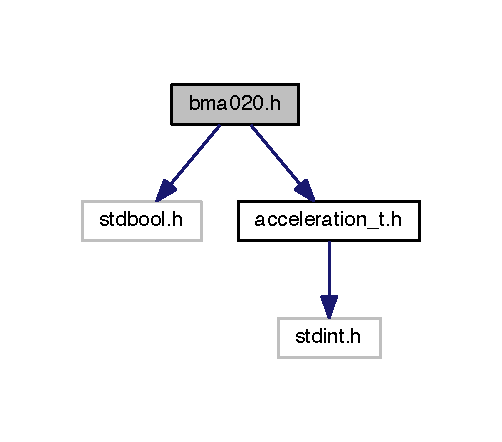
\includegraphics[width=241pt]{bma020_8h__incl}
\end{center}
\end{figure}
This graph shows which files directly or indirectly include this file\-:\nopagebreak
\begin{figure}[H]
\begin{center}
\leavevmode
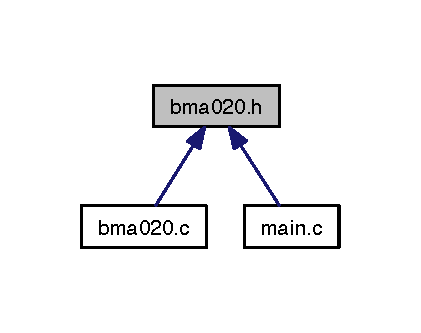
\includegraphics[width=202pt]{bma020_8h__dep__incl}
\end{center}
\end{figure}
\subsection*{Functions}
\begin{DoxyCompactItemize}
\item 
uint8\-\_\-t \hyperlink{bma020_8h_af61528e1bbdc91a9acac39c776cfc11b}{bma020\-\_\-get\-\_\-chip\-\_\-id} ()
\item 
uint8\-\_\-t \hyperlink{bma020_8h_ad815b4dc0e95fa9e9109930e4c1ba39a}{bma020\-\_\-get\-\_\-ml\-\_\-version} ()
\item 
uint8\-\_\-t \hyperlink{bma020_8h_a411ed87bf0eebcd6464a2efa0b303940}{bma020\-\_\-get\-\_\-ai\-\_\-version} ()
\item 
void \hyperlink{bma020_8h_aa049661ba05ba57de64bee327c9d668f}{bma020\-\_\-read\-\_\-raw\-\_\-acceleration} (\hyperlink{structacceleration__t}{acceleration\-\_\-t} $\ast$)
\item 
bool \hyperlink{bma020_8h_a5a11de6c62517d876636ffaaccbe99f8}{bma020\-\_\-is\-\_\-new\-\_\-data} (char)
\item 
bool \hyperlink{bma020_8h_af8352dba63a90d34734410f4f97eced4}{bma020\-\_\-get\-\_\-status\-\_\-hg} (void)
\item 
bool \hyperlink{bma020_8h_ab06787c50f090a339e8ed4d4a1408f6b}{bma020\-\_\-get\-\_\-status\-\_\-lg} (void)
\item 
bool \hyperlink{bma020_8h_a48178f75ec28ec3a881c0bd23ec16dfc}{bma020\-\_\-get\-\_\-lg\-\_\-latched} (void)
\item 
void \hyperlink{bma020_8h_aa591678c9c225c04379f31f443da516f}{bma020\-\_\-reset\-\_\-lg\-\_\-latched} (void)
\item 
bool \hyperlink{bma020_8h_a5607b1f4a151f90262f63ac79ec8dbd9}{bma020\-\_\-get\-\_\-hg\-\_\-latched} (void)
\item 
void \hyperlink{bma020_8h_a996664698b38ebcbdc5f35277c86271f}{bma020\-\_\-reset\-\_\-hg\-\_\-latched} (void)
\item 
bool \hyperlink{bma020_8h_ada7359286e7b2e8f5efe66dbc7e0ec3e}{bma020\-\_\-get\-\_\-alert\-\_\-phase} (void)
\item 
bool \hyperlink{bma020_8h_a225a6d888c491bc9eeaa587c71658530}{bma020\-\_\-get\-\_\-self\-\_\-test\-\_\-result} (void)
\item 
void \hyperlink{bma020_8h_ae46fb2b7063713e26d4f939a01c410b4}{bma020\-\_\-sleep} (void)
\item 
void \hyperlink{bma020_8h_aee5899ae2a2762d1f20c4f2895298e34}{bma020\-\_\-soft\-\_\-reset} (void)
\item 
void \hyperlink{bma020_8h_a1b4d80e962496fd3d254dc1adb060ccd}{bma020\-\_\-perform\-\_\-self\-\_\-test\-\_\-0} (void)
\item 
void \hyperlink{bma020_8h_aafad8d4b857d14f771e1b5584b540087}{bma020\-\_\-perform\-\_\-self\-\_\-test\-\_\-1} (void)
\item 
void \hyperlink{bma020_8h_a3060609bb2160962da7d73617c70b5a5}{bma020\-\_\-enable\-\_\-spi4} (bool)
\item 
bool \hyperlink{bma020_8h_a62a15f74e49f2463c1872dbe43dce521}{bma020\-\_\-is\-\_\-spi4} (void)
\item 
void \hyperlink{bma020_8h_aee001eb4d6bdaa5fb882d7063c289f64}{bma020\-\_\-disable\-\_\-shadow} (bool)
\item 
bool \hyperlink{bma020_8h_ad5d778ebe7f19ffc5447b05392bc81d5}{bma020\-\_\-is\-\_\-shadow\-\_\-disabled} (void)
\item 
void \hyperlink{bma020_8h_ac523767751ba8462faae363f828af936}{bma020\-\_\-reset\-\_\-interrupt} (void)
\item 
void \hyperlink{bma020_8h_aeafb1eaaefef0c0631616ee8bb1ba4b5}{bma020\-\_\-enable\-\_\-new\-\_\-data\-\_\-int} (bool)
\item 
bool \hyperlink{bma020_8h_a3f70726f60c671a6cd7250c84cc9ee7a}{bma020\-\_\-is\-\_\-new\-\_\-data\-\_\-int} (void)
\item 
void \hyperlink{bma020_8h_a308701ebfc10d9b112400a28736d43bb}{bma020\-\_\-enable\-\_\-lg} (bool)
\item 
bool \hyperlink{bma020_8h_a47004eaf6774aa870fd8e2d4d5c1ae80}{bma020\-\_\-is\-\_\-enable\-\_\-lg} (void)
\item 
void \hyperlink{bma020_8h_af1880cc730341de89b63540a43ee3430}{bma020\-\_\-enable\-\_\-hg} (bool)
\item 
bool \hyperlink{bma020_8h_a8bbc44dd5bf3320c9ea06ce54100fafc}{bma020\-\_\-is\-\_\-enable\-\_\-hg} (void)
\item 
void \hyperlink{bma020_8h_ae3589f40d1137a6b1837d58398c2ad0a}{bma020\-\_\-enable\-\_\-advanced\-\_\-int} (bool)
\item 
bool \hyperlink{bma020_8h_a7d48379dad99c291f448af6889a10c65}{bma020\-\_\-is\-\_\-advanced\-\_\-int} (void)
\item 
void \hyperlink{bma020_8h_af856d34c25ecc193c09ea7ed4573e4cf}{bma020\-\_\-enable\-\_\-any\-\_\-motion} (bool)
\item 
bool \hyperlink{bma020_8h_a7aaedcf13c31ab032c6014cf2f11d03e}{bma020\-\_\-is\-\_\-enable\-\_\-any\-\_\-motion} (void)
\item 
void \hyperlink{bma020_8h_ab1f89e73571acf071a07008e421a3a7d}{bma020\-\_\-enable\-\_\-motion\-\_\-alert} (bool)
\item 
bool \hyperlink{bma020_8h_a460b42665cb432f91a3e54c132f9891e}{bma020\-\_\-is\-\_\-enable\-\_\-motion\-\_\-alert} (void)
\item 
void \hyperlink{bma020_8h_a39c465b7b841da82750c106add157ee6}{bma020\-\_\-enable\-\_\-latched\-\_\-int} (bool)
\item 
bool \hyperlink{bma020_8h_a3e5636663c087915feeacb349b44ce31}{bma020\-\_\-is\-\_\-latched\-\_\-int} (void)
\item 
void \hyperlink{bma020_8h_ab3fa54af803bedc74927f8f2cf00aedc}{bma020\-\_\-set\-\_\-lg\-\_\-threshold} (uint8\-\_\-t threshold)
\item 
uint8\-\_\-t \hyperlink{bma020_8h_ab9c52c7427ba44b7f40c7de7effd6b70}{bma020\-\_\-get\-\_\-lg\-\_\-threshold} ()
\item 
void \hyperlink{bma020_8h_a9c88ac2767f5099da4bceb35d5185247}{bma020\-\_\-set\-\_\-lg\-\_\-duration} (uint8\-\_\-t)
\item 
uint8\-\_\-t \hyperlink{bma020_8h_af3021e4c25165a76c664be19c968ed7a}{bma020\-\_\-get\-\_\-lg\-\_\-duration} ()
\item 
bool \hyperlink{bma020_8h_a0925a60b0799b1f000b04d026027e626}{bma020\-\_\-set\-\_\-counter\-\_\-lg} (uint8\-\_\-t)
\item 
uint8\-\_\-t \hyperlink{bma020_8h_a851c0bbf26d7d95e294beae813e2c6f8}{bma020\-\_\-get\-\_\-counter\-\_\-lg} (void)
\item 
void \hyperlink{bma020_8h_acf15f8f2a17ea937719f4f49af0c019f}{bma020\-\_\-set\-\_\-lg\-\_\-hysterese} (uint8\-\_\-t hysterese)
\item 
uint8\-\_\-t \hyperlink{bma020_8h_a73397e5a2d7ec9443c34e9f2fd4e7e8e}{bma020\-\_\-get\-\_\-lg\-\_\-hysterese} (void)
\item 
void \hyperlink{bma020_8h_ab9b82b4d29bd5c0d921903469a1ceae3}{bma020\-\_\-set\-\_\-hg\-\_\-threshold} (uint8\-\_\-t)
\item 
uint8\-\_\-t \hyperlink{bma020_8h_a7574ff05e7bc504eb37df267bd1a6d54}{bma020\-\_\-get\-\_\-hg\-\_\-threshold} ()
\item 
void \hyperlink{bma020_8h_aa7bb61399c444a272182bcb266d36b35}{bma020\-\_\-set\-\_\-hg\-\_\-duration} (uint8\-\_\-t)
\item 
uint8\-\_\-t \hyperlink{bma020_8h_a298d59459d1e3fd4a27ad187027ecea2}{bma020\-\_\-get\-\_\-hg\-\_\-duration} ()
\item 
bool \hyperlink{bma020_8h_acc8c5b0f1114ea09cd6653d2d7e3fb38}{bma020\-\_\-set\-\_\-counter\-\_\-hg} (uint8\-\_\-t)
\item 
uint8\-\_\-t \hyperlink{bma020_8h_aec5666921548a0d1a7c81c9b71dd9d44}{bma020\-\_\-get\-\_\-counter\-\_\-hg} (void)
\item 
void \hyperlink{bma020_8h_a24882f81d49e4db67665fb7d74bed976}{bma020\-\_\-set\-\_\-hg\-\_\-hysterese} (uint8\-\_\-t)
\item 
uint8\-\_\-t \hyperlink{bma020_8h_a532014744107ba2e88a56d2c4119db40}{bma020\-\_\-get\-\_\-hg\-\_\-hysterese} (void)
\item 
void \hyperlink{bma020_8h_a2fb9ce02a8f8f96bea6822dacb3dbdda}{bma020\-\_\-set\-\_\-any\-\_\-motion\-\_\-threshold} (uint8\-\_\-t)
\item 
uint8\-\_\-t \hyperlink{bma020_8h_aa886f09ffd7a8a7237198a56ee262fc5}{bma020\-\_\-get\-\_\-any\-\_\-motion\-\_\-threshold} (void)
\item 
bool \hyperlink{bma020_8h_a2fa0d7fb2232f63015927a4411b6936f}{bma020\-\_\-set\-\_\-any\-\_\-motion\-\_\-duration} (uint8\-\_\-t)
\item 
uint8\-\_\-t \hyperlink{bma020_8h_aa0957d9a759593bf02c37f61dac4a41b}{bma020\-\_\-get\-\_\-any\-\_\-motion\-\_\-duration} (void)
\item 
void \hyperlink{bma020_8h_a84ad4c88f3a38ec91b3639e58ded55ae}{bma020\-\_\-enable\-\_\-wake\-\_\-up} (bool enable)
\item 
bool \hyperlink{bma020_8h_a754386a5ed68093f02f5bec3f5e98cbd}{bma020\-\_\-is\-\_\-wake\-\_\-up} (void)
\item 
bool \hyperlink{bma020_8h_ae73261ee46188952993f69970854e386}{bma020\-\_\-set\-\_\-wake\-\_\-up\-\_\-pause} (uint16\-\_\-t wake\-\_\-up\-\_\-time)
\item 
uint16\-\_\-t \hyperlink{bma020_8h_a9e076fdb4daec0fe8352340385006b7d}{bma020\-\_\-get\-\_\-wake\-\_\-up\-\_\-pause} (void)
\item 
uint16\-\_\-t \hyperlink{bma020_8h_a7638286b73693422b67c4fabef32fe24}{bma020\-\_\-get\-\_\-bandwidth} (void)
\item 
bool \hyperlink{bma020_8h_a9bd3b24299e9db9b1444ec92790b3e68}{bma020\-\_\-set\-\_\-bandwidth} (uint16\-\_\-t)
\item 
uint8\-\_\-t \hyperlink{bma020_8h_a9a0c0e161ae1c7ac0963a98f1a499c00}{bma020\-\_\-get\-\_\-range} (void)
\item 
bool \hyperlink{bma020_8h_ac7f7e61919fd9f19b2620e2009fad92c}{bma020\-\_\-set\-\_\-range} (uint8\-\_\-t)
\item 
void \hyperlink{bma020_8h_af0a438e715f02efa689bc251ccbb8050}{bma020\-\_\-set\-\_\-customer\-\_\-reserved\-\_\-1} (uint8\-\_\-t value)
\item 
uint8\-\_\-t \hyperlink{bma020_8h_a772e31e89870de0eebfdf2d00bbf145a}{bma020\-\_\-get\-\_\-customer\-\_\-reserved\-\_\-1} ()
\item 
void \hyperlink{bma020_8h_aff774b72ecf7cfae5dd7855cac989953}{bma020\-\_\-set\-\_\-customer\-\_\-reserved\-\_\-2} (uint8\-\_\-t value)
\item 
uint8\-\_\-t \hyperlink{bma020_8h_a57c220a687c54813b3971dbb53e4d341}{bma020\-\_\-get\-\_\-customer\-\_\-reserved\-\_\-2} ()
\item 
void \hyperlink{bma020_8h_ac5c1a01ed031d3c8826f4a54cbae6efe}{bma020\-\_\-init} (void)
\end{DoxyCompactItemize}


\subsection{Detailed Description}
This modul implements a low level driver for the bma020 acceleration sensor. All registers and flags are accessable through functions. But the readed acceleration values arn't filterd or calibrated. This must be implemented on a higer level of abstraction. Alexander Mertens (\href{mailto:alexander.mertens@stud.fh-dortmund.de}{\tt alexander.\-mertens@stud.\-fh-\/dortmund.\-de}) \begin{DoxyDate}{Date}
06.\-11.\-2013 Detailed description of file. 
\end{DoxyDate}


Definition in file \hyperlink{bma020_8h_source}{bma020.\-h}.



\subsection{Function Documentation}
\hypertarget{bma020_8h_aee001eb4d6bdaa5fb882d7063c289f64}{\index{bma020.\-h@{bma020.\-h}!bma020\-\_\-disable\-\_\-shadow@{bma020\-\_\-disable\-\_\-shadow}}
\index{bma020\-\_\-disable\-\_\-shadow@{bma020\-\_\-disable\-\_\-shadow}!bma020.h@{bma020.\-h}}
\subsubsection[{bma020\-\_\-disable\-\_\-shadow}]{\setlength{\rightskip}{0pt plus 5cm}void bma020\-\_\-disable\-\_\-shadow (
\begin{DoxyParamCaption}
\item[{bool}]{disable}
\end{DoxyParamCaption}
)}}\label{bma020_8h_aee001eb4d6bdaa5fb882d7063c289f64}
B\-M\-A020 provides the possibility to block the update of data M\-S\-B while L\-S\-B are read out. This avoids a potential mixing of L\-S\-B and M\-S\-B of successive conversion cycles. When this bit (address 15h, bit 3) is at 1, the blocking procedure for M\-S\-B is not realized and M\-S\-B only reading is possible. 
\begin{DoxyParams}{Parameters}
{\em disable} & \\
\hline
\end{DoxyParams}


Definition at line 463 of file bma020.\-c.



References B\-M\-A020\-\_\-\-B\-I\-T\-\_\-\-S\-H\-A\-D\-O\-W\-\_\-\-D\-I\-S, and B\-M\-A020\-\_\-\-R\-E\-G\-I\-S\-T\-E\-R\-\_\-\-C\-O\-N\-T\-R\-O\-L\-\_\-\-S\-P\-I4\-\_\-\-I\-N\-T\-E\-R\-R\-U\-P\-T\-\_\-\-W\-A\-K\-E\-U\-P.

\hypertarget{bma020_8h_ae3589f40d1137a6b1837d58398c2ad0a}{\index{bma020.\-h@{bma020.\-h}!bma020\-\_\-enable\-\_\-advanced\-\_\-int@{bma020\-\_\-enable\-\_\-advanced\-\_\-int}}
\index{bma020\-\_\-enable\-\_\-advanced\-\_\-int@{bma020\-\_\-enable\-\_\-advanced\-\_\-int}!bma020.h@{bma020.\-h}}
\subsubsection[{bma020\-\_\-enable\-\_\-advanced\-\_\-int}]{\setlength{\rightskip}{0pt plus 5cm}void bma020\-\_\-enable\-\_\-advanced\-\_\-int (
\begin{DoxyParamCaption}
\item[{bool}]{enable}
\end{DoxyParamCaption}
)}}\label{bma020_8h_ae3589f40d1137a6b1837d58398c2ad0a}
This bit (address 15h, bit 6) is used to disable advanced interrupt control bits (any\-\_\-motion, alert). If enable\-\_\-adv\-\_\-\-I\-N\-T=0, writing to these bits has no effect on sensor I\-C function. 
\begin{DoxyParams}{Parameters}
{\em enable} & \\
\hline
\end{DoxyParams}


Definition at line 579 of file bma020.\-c.



References B\-M\-A020\-\_\-\-B\-I\-T\-\_\-\-A\-D\-V\-A\-N\-C\-E\-D\-\_\-\-I\-N\-T, and B\-M\-A020\-\_\-\-R\-E\-G\-I\-S\-T\-E\-R\-\_\-\-C\-O\-N\-T\-R\-O\-L\-\_\-\-S\-P\-I4\-\_\-\-I\-N\-T\-E\-R\-R\-U\-P\-T\-\_\-\-W\-A\-K\-E\-U\-P.

\hypertarget{bma020_8h_af856d34c25ecc193c09ea7ed4573e4cf}{\index{bma020.\-h@{bma020.\-h}!bma020\-\_\-enable\-\_\-any\-\_\-motion@{bma020\-\_\-enable\-\_\-any\-\_\-motion}}
\index{bma020\-\_\-enable\-\_\-any\-\_\-motion@{bma020\-\_\-enable\-\_\-any\-\_\-motion}!bma020.h@{bma020.\-h}}
\subsubsection[{bma020\-\_\-enable\-\_\-any\-\_\-motion}]{\setlength{\rightskip}{0pt plus 5cm}void bma020\-\_\-enable\-\_\-any\-\_\-motion (
\begin{DoxyParamCaption}
\item[{bool}]{enable}
\end{DoxyParamCaption}
)}}\label{bma020_8h_af856d34c25ecc193c09ea7ed4573e4cf}
This bit ((address 0\-Bh, bit 6)enables the any motion criteria to generate directly an interrupt. It can not be turned on simultaneously with alert. This bit can be masked by enable\-\_\- adv\-\_\-\-I\-N\-T, the value of this bit is ignored when enable\-\_\-adv\-\_\-\-I\-N\-T=0 (section 3.\-2.\-3).


\begin{DoxyParams}{Parameters}
{\em enable} & \\
\hline
\end{DoxyParams}


Definition at line 607 of file bma020.\-c.



References B\-M\-A020\-\_\-\-B\-I\-T\-\_\-\-A\-N\-Y\-\_\-\-M\-O\-T\-I\-O\-N, and B\-M\-A020\-\_\-\-R\-E\-G\-I\-S\-T\-E\-R\-\_\-\-A\-L\-E\-R\-T\-\_\-\-E\-N\-A\-N\-Y\-M\-O\-T\-I\-O\-N\-\_\-\-C\-N\-T\-H\-G\-\_\-\-C\-N\-T\-L\-G\-\_\-\-E\-N\-H\-G\-\_\-\-E\-N\-L\-G.

\hypertarget{bma020_8h_af1880cc730341de89b63540a43ee3430}{\index{bma020.\-h@{bma020.\-h}!bma020\-\_\-enable\-\_\-hg@{bma020\-\_\-enable\-\_\-hg}}
\index{bma020\-\_\-enable\-\_\-hg@{bma020\-\_\-enable\-\_\-hg}!bma020.h@{bma020.\-h}}
\subsubsection[{bma020\-\_\-enable\-\_\-hg}]{\setlength{\rightskip}{0pt plus 5cm}void bma020\-\_\-enable\-\_\-hg (
\begin{DoxyParamCaption}
\item[{bool}]{enable}
\end{DoxyParamCaption}
)}}\label{bma020_8h_af1880cc730341de89b63540a43ee3430}
This bit (address 0\-Bh, bit 1) enables the H\-G\-\_\-thres criteria to generate an interrupt. 
\begin{DoxyParams}{Parameters}
{\em enable} & \\
\hline
\end{DoxyParams}


Definition at line 552 of file bma020.\-c.



References B\-M\-A020\-\_\-\-B\-I\-T\-\_\-\-E\-N\-A\-B\-L\-E\-\_\-\-H\-G, and B\-M\-A020\-\_\-\-R\-E\-G\-I\-S\-T\-E\-R\-\_\-\-A\-L\-E\-R\-T\-\_\-\-E\-N\-A\-N\-Y\-M\-O\-T\-I\-O\-N\-\_\-\-C\-N\-T\-H\-G\-\_\-\-C\-N\-T\-L\-G\-\_\-\-E\-N\-H\-G\-\_\-\-E\-N\-L\-G.

\hypertarget{bma020_8h_a39c465b7b841da82750c106add157ee6}{\index{bma020.\-h@{bma020.\-h}!bma020\-\_\-enable\-\_\-latched\-\_\-int@{bma020\-\_\-enable\-\_\-latched\-\_\-int}}
\index{bma020\-\_\-enable\-\_\-latched\-\_\-int@{bma020\-\_\-enable\-\_\-latched\-\_\-int}!bma020.h@{bma020.\-h}}
\subsubsection[{bma020\-\_\-enable\-\_\-latched\-\_\-int}]{\setlength{\rightskip}{0pt plus 5cm}void bma020\-\_\-enable\-\_\-latched\-\_\-int (
\begin{DoxyParamCaption}
\item[{bool}]{enable}
\end{DoxyParamCaption}
)}}\label{bma020_8h_a39c465b7b841da82750c106add157ee6}
If this bit (address 15h, bit 4) is at 1, interrupts are latched. The I\-N\-T pad stays high until microprocessor detects it and writes reset\-\_\-\-I\-N\-T control bit to 1 (section 3.\-3.\-1). When this bit is at 0, interrupts are set and reset directly by B\-M\-A020 according to programmable criteria (sections 3.\-2.\-7 and 3.\-2.\-8). 
\begin{DoxyParams}{Parameters}
{\em enable} & \\
\hline
\end{DoxyParams}


Definition at line 662 of file bma020.\-c.



References B\-M\-A020\-\_\-\-B\-I\-T\-\_\-\-L\-A\-T\-C\-H\-\_\-\-I\-N\-T, and B\-M\-A020\-\_\-\-R\-E\-G\-I\-S\-T\-E\-R\-\_\-\-C\-O\-N\-T\-R\-O\-L\-\_\-\-S\-P\-I4\-\_\-\-I\-N\-T\-E\-R\-R\-U\-P\-T\-\_\-\-W\-A\-K\-E\-U\-P.

\hypertarget{bma020_8h_a308701ebfc10d9b112400a28736d43bb}{\index{bma020.\-h@{bma020.\-h}!bma020\-\_\-enable\-\_\-lg@{bma020\-\_\-enable\-\_\-lg}}
\index{bma020\-\_\-enable\-\_\-lg@{bma020\-\_\-enable\-\_\-lg}!bma020.h@{bma020.\-h}}
\subsubsection[{bma020\-\_\-enable\-\_\-lg}]{\setlength{\rightskip}{0pt plus 5cm}void bma020\-\_\-enable\-\_\-lg (
\begin{DoxyParamCaption}
\item[{bool}]{enable}
\end{DoxyParamCaption}
)}}\label{bma020_8h_a308701ebfc10d9b112400a28736d43bb}
This bit (address 0\-Bh, bit 0) enables the L\-G\-\_\-thres criteria to generate an interrupt. 

Definition at line 526 of file bma020.\-c.



References B\-M\-A020\-\_\-\-B\-I\-T\-\_\-\-E\-N\-A\-B\-L\-E\-\_\-\-L\-G, and B\-M\-A020\-\_\-\-R\-E\-G\-I\-S\-T\-E\-R\-\_\-\-A\-L\-E\-R\-T\-\_\-\-E\-N\-A\-N\-Y\-M\-O\-T\-I\-O\-N\-\_\-\-C\-N\-T\-H\-G\-\_\-\-C\-N\-T\-L\-G\-\_\-\-E\-N\-H\-G\-\_\-\-E\-N\-L\-G.

\hypertarget{bma020_8h_ab1f89e73571acf071a07008e421a3a7d}{\index{bma020.\-h@{bma020.\-h}!bma020\-\_\-enable\-\_\-motion\-\_\-alert@{bma020\-\_\-enable\-\_\-motion\-\_\-alert}}
\index{bma020\-\_\-enable\-\_\-motion\-\_\-alert@{bma020\-\_\-enable\-\_\-motion\-\_\-alert}!bma020.h@{bma020.\-h}}
\subsubsection[{bma020\-\_\-enable\-\_\-motion\-\_\-alert}]{\setlength{\rightskip}{0pt plus 5cm}void bma020\-\_\-enable\-\_\-motion\-\_\-alert (
\begin{DoxyParamCaption}
\item[{bool}]{enable}
\end{DoxyParamCaption}
)}}\label{bma020_8h_ab1f89e73571acf071a07008e421a3a7d}
f this bit (address 0\-Bh, bit 7) is at 1, the any\-\_\-motion criterion will set B\-M\-A020 into alert mode (section 3.\-2.\-9). This bit can be masked by enable\-\_\-adv\-\_\-\-I\-N\-T, the value of this bit is ignored when enable\-\_\-adv\-\_\-\-I\-N\-T=0 (section 3.\-2.\-3).


\begin{DoxyParams}{Parameters}
{\em enable} & \\
\hline
\end{DoxyParams}


Definition at line 634 of file bma020.\-c.



References B\-M\-A020\-\_\-\-B\-I\-T\-\_\-\-A\-L\-T\-E\-R\-T, and B\-M\-A020\-\_\-\-R\-E\-G\-I\-S\-T\-E\-R\-\_\-\-A\-L\-E\-R\-T\-\_\-\-E\-N\-A\-N\-Y\-M\-O\-T\-I\-O\-N\-\_\-\-C\-N\-T\-H\-G\-\_\-\-C\-N\-T\-L\-G\-\_\-\-E\-N\-H\-G\-\_\-\-E\-N\-L\-G.

\hypertarget{bma020_8h_aeafb1eaaefef0c0631616ee8bb1ba4b5}{\index{bma020.\-h@{bma020.\-h}!bma020\-\_\-enable\-\_\-new\-\_\-data\-\_\-int@{bma020\-\_\-enable\-\_\-new\-\_\-data\-\_\-int}}
\index{bma020\-\_\-enable\-\_\-new\-\_\-data\-\_\-int@{bma020\-\_\-enable\-\_\-new\-\_\-data\-\_\-int}!bma020.h@{bma020.\-h}}
\subsubsection[{bma020\-\_\-enable\-\_\-new\-\_\-data\-\_\-int}]{\setlength{\rightskip}{0pt plus 5cm}void bma020\-\_\-enable\-\_\-new\-\_\-data\-\_\-int (
\begin{DoxyParamCaption}
\item[{bool}]{enable}
\end{DoxyParamCaption}
)}}\label{bma020_8h_aeafb1eaaefef0c0631616ee8bb1ba4b5}
If this bit (address 15h, bit 5) is set to 1, an interrupt will be generated when all three axes acceleration values are new, i.\-e. B\-M\-A020 updated all acceleration values after latest serial read-\/out. Interrupt generated from new data detection is a latched one; microcontroller has to write reset\-\_\-\-I\-N\-T at 1 after interrupt has been detected high (section 3.\-3.\-1). This interrupt is also reset by any acceleration byte read procedure (read access to address 02h to 07h). New data interrupt always occurs at the end of the Z-\/axis value update in the output register (3k\-Hz rate). Following figure shows two examples of X-\/axis read out and the corresponding interrupt generation. 
\begin{DoxyParams}{Parameters}
{\em enable} & \\
\hline
\end{DoxyParams}


Definition at line 505 of file bma020.\-c.



References B\-M\-A020\-\_\-\-B\-I\-T\-\_\-\-N\-E\-W\-\_\-\-D\-A\-T\-A\-\_\-\-I\-N\-T, and B\-M\-A020\-\_\-\-R\-E\-G\-I\-S\-T\-E\-R\-\_\-\-C\-O\-N\-T\-R\-O\-L\-\_\-\-S\-P\-I4\-\_\-\-I\-N\-T\-E\-R\-R\-U\-P\-T\-\_\-\-W\-A\-K\-E\-U\-P.

\hypertarget{bma020_8h_a3060609bb2160962da7d73617c70b5a5}{\index{bma020.\-h@{bma020.\-h}!bma020\-\_\-enable\-\_\-spi4@{bma020\-\_\-enable\-\_\-spi4}}
\index{bma020\-\_\-enable\-\_\-spi4@{bma020\-\_\-enable\-\_\-spi4}!bma020.h@{bma020.\-h}}
\subsubsection[{bma020\-\_\-enable\-\_\-spi4}]{\setlength{\rightskip}{0pt plus 5cm}void bma020\-\_\-enable\-\_\-spi4 (
\begin{DoxyParamCaption}
\item[{bool}]{enable}
\end{DoxyParamCaption}
)}}\label{bma020_8h_a3060609bb2160962da7d73617c70b5a5}
The S\-P\-I4 bit ((address 15h, bit 7) is used to select the correct S\-P\-I protocol (three-\/wire or four-\/ wire, S\-P\-I-\/mode 3). The default value is S\-P\-I4=1 (four-\/wire S\-P\-I is default value). After power on reset or soft reset it is recommended to set the S\-P\-I4-\/bit to the correct value. This first writing is possible because only C\-S\-B, S\-C\-K and S\-D\-I are required for a write sequence and the 3 bit timing diagrams are identical in three-\/wire and four-\/wire configuration.

Recommended procedure\-: Set S\-P\-I4 to the correct value (S\-P\-I4=0 for S\-P\-I three-\/wire, S\-P\-I4=1 for S\-P\-I four-\/wire (=default)) every time after power on reset or soft reset. 
\begin{DoxyParams}{Parameters}
{\em enable} & \\
\hline
\end{DoxyParams}


Definition at line 437 of file bma020.\-c.



References B\-M\-A020\-\_\-\-B\-I\-T\-\_\-\-S\-P\-I4, and B\-M\-A020\-\_\-\-R\-E\-G\-I\-S\-T\-E\-R\-\_\-\-C\-O\-N\-T\-R\-O\-L\-\_\-\-S\-P\-I4\-\_\-\-I\-N\-T\-E\-R\-R\-U\-P\-T\-\_\-\-W\-A\-K\-E\-U\-P.

\hypertarget{bma020_8h_a84ad4c88f3a38ec91b3639e58ded55ae}{\index{bma020.\-h@{bma020.\-h}!bma020\-\_\-enable\-\_\-wake\-\_\-up@{bma020\-\_\-enable\-\_\-wake\-\_\-up}}
\index{bma020\-\_\-enable\-\_\-wake\-\_\-up@{bma020\-\_\-enable\-\_\-wake\-\_\-up}!bma020.h@{bma020.\-h}}
\subsubsection[{bma020\-\_\-enable\-\_\-wake\-\_\-up}]{\setlength{\rightskip}{0pt plus 5cm}void bma020\-\_\-enable\-\_\-wake\-\_\-up (
\begin{DoxyParamCaption}
\item[{bool}]{enable}
\end{DoxyParamCaption}
)}}\label{bma020_8h_a84ad4c88f3a38ec91b3639e58ded55ae}
This bit (address 15h, bit 0) makes B\-M\-A020 automatically switching from sleep mode to normal mode after the delay defined by wake\-\_\-up\-\_\-pause (section 3.\-1.\-5). When the sensor I\-C goes from sleep to normal mode, it starts acceleration acquisition and performs interrupt verification (section 3.\-2). The sensor I\-C automatically switches back from normal to sleep mode again if no fulfilment of programmed interrupt criteria has been detected. The I\-C wakes-\/up for a minimum duration which depends on the number of required valid acceleration data to determine if an interrupt should be generated.

If a latched interrupt is generated, this can be used to wake-\/up a microprocessor. The sensor I\-C will wait for a reset\-\_\-\-I\-N\-T command and restart interrupt verification. B\-M\-A020 can not go back to sleep mode if reset\-\_\-\-I\-N\-T is not issued after a latched interrupt.

If a not-\/latched interrupt is generated, the device waits in the normal mode till the interrupt condition disappears. The minimum duration of interrupt activation is 330microsecs. If no interrupt is generated, the sensor I\-C goes to sleep mode for a defined time (wake\-\_\-up\-\_\-pause). For more details on the wake-\/up functionality, please refer to chapter 7.\-3


\begin{DoxyParams}{Parameters}
{\em enable} & \\
\hline
\end{DoxyParams}


Definition at line 1131 of file bma020.\-c.



References B\-M\-A020\-\_\-\-B\-I\-T\-\_\-\-W\-A\-K\-E\-\_\-\-U\-P, and B\-M\-A020\-\_\-\-R\-E\-G\-I\-S\-T\-E\-R\-\_\-\-C\-O\-N\-T\-R\-O\-L\-\_\-\-S\-P\-I4\-\_\-\-I\-N\-T\-E\-R\-R\-U\-P\-T\-\_\-\-W\-A\-K\-E\-U\-P.

\hypertarget{bma020_8h_a411ed87bf0eebcd6464a2efa0b303940}{\index{bma020.\-h@{bma020.\-h}!bma020\-\_\-get\-\_\-ai\-\_\-version@{bma020\-\_\-get\-\_\-ai\-\_\-version}}
\index{bma020\-\_\-get\-\_\-ai\-\_\-version@{bma020\-\_\-get\-\_\-ai\-\_\-version}!bma020.h@{bma020.\-h}}
\subsubsection[{bma020\-\_\-get\-\_\-ai\-\_\-version}]{\setlength{\rightskip}{0pt plus 5cm}uint8\-\_\-t bma020\-\_\-get\-\_\-ai\-\_\-version (
\begin{DoxyParamCaption}
{}
\end{DoxyParamCaption}
)}}\label{bma020_8h_a411ed87bf0eebcd6464a2efa0b303940}
A\-L Version is used with M\-L Version to identify the chip revision \begin{DoxyReturn}{Returns}
A\-L Version 
\end{DoxyReturn}


Definition at line 145 of file bma020.\-c.



References B\-M\-A020\-\_\-\-R\-E\-G\-I\-S\-T\-E\-R\-\_\-\-V\-E\-R\-S\-I\-O\-N.

\hypertarget{bma020_8h_ada7359286e7b2e8f5efe66dbc7e0ec3e}{\index{bma020.\-h@{bma020.\-h}!bma020\-\_\-get\-\_\-alert\-\_\-phase@{bma020\-\_\-get\-\_\-alert\-\_\-phase}}
\index{bma020\-\_\-get\-\_\-alert\-\_\-phase@{bma020\-\_\-get\-\_\-alert\-\_\-phase}!bma020.h@{bma020.\-h}}
\subsubsection[{bma020\-\_\-get\-\_\-alert\-\_\-phase}]{\setlength{\rightskip}{0pt plus 5cm}bool bma020\-\_\-get\-\_\-alert\-\_\-phase (
\begin{DoxyParamCaption}
\item[{void}]{}
\end{DoxyParamCaption}
)}}\label{bma020_8h_ada7359286e7b2e8f5efe66dbc7e0ec3e}
This function returns ture, if alert mode is activated and an any motion criterion has been detected. During alert phase, H\-G\-\_\-dur and L\-G\-\_\-dur variables are decreased to have a smaller reaction time when H\-G\-\_\-thres and L\-G\-\_\-thres thresholds are crossed; the decrease rate is by 1 ms per ms.\-The alert mode is reset when an interrupt generated due to a high threshold or a low threshold event or when both H\-G\-\_\-dur and L\-G\-\_\-dur variables are at 0. When alert is reset, H\-G\-\_\-dur and L\-G\-\_\-dur variables come back to their original values stored in image registers. \begin{DoxyReturn}{Returns}
true if alare criterias are fullified 
\end{DoxyReturn}


Definition at line 326 of file bma020.\-c.



References B\-M\-A020\-\_\-\-B\-I\-T\-\_\-\-A\-L\-E\-R\-T\-\_\-\-P\-H\-A\-S\-E, and B\-M\-A020\-\_\-\-R\-E\-G\-I\-S\-T\-E\-R\-\_\-\-S\-T\-A\-T\-U\-S.

\hypertarget{bma020_8h_aa0957d9a759593bf02c37f61dac4a41b}{\index{bma020.\-h@{bma020.\-h}!bma020\-\_\-get\-\_\-any\-\_\-motion\-\_\-duration@{bma020\-\_\-get\-\_\-any\-\_\-motion\-\_\-duration}}
\index{bma020\-\_\-get\-\_\-any\-\_\-motion\-\_\-duration@{bma020\-\_\-get\-\_\-any\-\_\-motion\-\_\-duration}!bma020.h@{bma020.\-h}}
\subsubsection[{bma020\-\_\-get\-\_\-any\-\_\-motion\-\_\-duration}]{\setlength{\rightskip}{0pt plus 5cm}uint8\-\_\-t bma020\-\_\-get\-\_\-any\-\_\-motion\-\_\-duration (
\begin{DoxyParamCaption}
\item[{void}]{}
\end{DoxyParamCaption}
)}}\label{bma020_8h_aa0957d9a759593bf02c37f61dac4a41b}


Definition at line 1083 of file bma020.\-c.



References B\-M\-A020\-\_\-\-B\-I\-T\-\_\-\-A\-N\-Y\-\_\-\-M\-O\-T\-I\-O\-N\-\_\-\-D\-U\-R\-A\-T\-I\-O\-N\-\_\-0, B\-M\-A020\-\_\-\-B\-I\-T\-\_\-\-A\-N\-Y\-\_\-\-M\-O\-T\-I\-O\-N\-\_\-\-D\-U\-R\-A\-T\-I\-O\-N\-\_\-1, and B\-M\-A020\-\_\-\-R\-E\-G\-I\-S\-T\-E\-R\-\_\-\-A\-M\-D\-U\-R\-\_\-\-H\-G\-H\-Y\-S\-\_\-\-L\-G\-H\-Y\-S.

\hypertarget{bma020_8h_aa886f09ffd7a8a7237198a56ee262fc5}{\index{bma020.\-h@{bma020.\-h}!bma020\-\_\-get\-\_\-any\-\_\-motion\-\_\-threshold@{bma020\-\_\-get\-\_\-any\-\_\-motion\-\_\-threshold}}
\index{bma020\-\_\-get\-\_\-any\-\_\-motion\-\_\-threshold@{bma020\-\_\-get\-\_\-any\-\_\-motion\-\_\-threshold}!bma020.h@{bma020.\-h}}
\subsubsection[{bma020\-\_\-get\-\_\-any\-\_\-motion\-\_\-threshold}]{\setlength{\rightskip}{0pt plus 5cm}uint8\-\_\-t bma020\-\_\-get\-\_\-any\-\_\-motion\-\_\-threshold (
\begin{DoxyParamCaption}
\item[{void}]{}
\end{DoxyParamCaption}
)}}\label{bma020_8h_aa886f09ffd7a8a7237198a56ee262fc5}
returns any motion threshold \begin{DoxyReturn}{Returns}

\end{DoxyReturn}


Definition at line 1038 of file bma020.\-c.



References B\-M\-A020\-\_\-\-R\-E\-G\-I\-S\-T\-E\-R\-\_\-\-A\-N\-Y\-\_\-\-M\-O\-T\-I\-O\-N\-\_\-\-T\-H\-R\-E\-S\-H\-O\-L\-D.

\hypertarget{bma020_8h_a7638286b73693422b67c4fabef32fe24}{\index{bma020.\-h@{bma020.\-h}!bma020\-\_\-get\-\_\-bandwidth@{bma020\-\_\-get\-\_\-bandwidth}}
\index{bma020\-\_\-get\-\_\-bandwidth@{bma020\-\_\-get\-\_\-bandwidth}!bma020.h@{bma020.\-h}}
\subsubsection[{bma020\-\_\-get\-\_\-bandwidth}]{\setlength{\rightskip}{0pt plus 5cm}uint16\-\_\-t bma020\-\_\-get\-\_\-bandwidth (
\begin{DoxyParamCaption}
\item[{void}]{}
\end{DoxyParamCaption}
)}}\label{bma020_8h_a7638286b73693422b67c4fabef32fe24}
returns the current bandwidth \begin{DoxyReturn}{Returns}

\end{DoxyReturn}


Definition at line 1299 of file bma020.\-c.



References B\-M\-A020\-\_\-\-B\-I\-T\-\_\-\-B\-A\-N\-D\-W\-I\-D\-T\-H\-\_\-0, B\-M\-A020\-\_\-\-B\-I\-T\-\_\-\-B\-A\-N\-D\-W\-I\-D\-T\-H\-\_\-1, B\-M\-A020\-\_\-\-B\-I\-T\-\_\-\-B\-A\-N\-D\-W\-I\-D\-T\-H\-\_\-2, and B\-M\-A020\-\_\-\-R\-E\-G\-I\-S\-T\-E\-R\-\_\-\-C\-O\-N\-T\-R\-O\-L\-\_\-\-R\-A\-N\-G\-E\-\_\-\-B\-A\-N\-D\-W\-I\-D\-T\-H.

\hypertarget{bma020_8h_af61528e1bbdc91a9acac39c776cfc11b}{\index{bma020.\-h@{bma020.\-h}!bma020\-\_\-get\-\_\-chip\-\_\-id@{bma020\-\_\-get\-\_\-chip\-\_\-id}}
\index{bma020\-\_\-get\-\_\-chip\-\_\-id@{bma020\-\_\-get\-\_\-chip\-\_\-id}!bma020.h@{bma020.\-h}}
\subsubsection[{bma020\-\_\-get\-\_\-chip\-\_\-id}]{\setlength{\rightskip}{0pt plus 5cm}uint8\-\_\-t bma020\-\_\-get\-\_\-chip\-\_\-id (
\begin{DoxyParamCaption}
{}
\end{DoxyParamCaption}
)}}\label{bma020_8h_af61528e1bbdc91a9acac39c776cfc11b}
The Chip I\-D is used by customer to be able to recognize B\-M\-A020. This code is fixed to 010b. \begin{DoxyReturn}{Returns}
Chip I\-D 
\end{DoxyReturn}


Definition at line 118 of file bma020.\-c.



References B\-M\-A020\-\_\-\-R\-E\-G\-I\-S\-T\-E\-R\-\_\-\-V\-E\-R\-S\-I\-O\-N.

\hypertarget{bma020_8h_aec5666921548a0d1a7c81c9b71dd9d44}{\index{bma020.\-h@{bma020.\-h}!bma020\-\_\-get\-\_\-counter\-\_\-hg@{bma020\-\_\-get\-\_\-counter\-\_\-hg}}
\index{bma020\-\_\-get\-\_\-counter\-\_\-hg@{bma020\-\_\-get\-\_\-counter\-\_\-hg}!bma020.h@{bma020.\-h}}
\subsubsection[{bma020\-\_\-get\-\_\-counter\-\_\-hg}]{\setlength{\rightskip}{0pt plus 5cm}uint8\-\_\-t bma020\-\_\-get\-\_\-counter\-\_\-hg (
\begin{DoxyParamCaption}
\item[{void}]{}
\end{DoxyParamCaption}
)}}\label{bma020_8h_aec5666921548a0d1a7c81c9b71dd9d44}
returns the current counter \begin{DoxyReturn}{Returns}

\end{DoxyReturn}


Definition at line 954 of file bma020.\-c.



References B\-M\-A020\-\_\-\-B\-I\-T\-\_\-\-C\-O\-U\-N\-T\-E\-R\-\_\-\-H\-G\-\_\-0, B\-M\-A020\-\_\-\-B\-I\-T\-\_\-\-C\-O\-U\-N\-T\-E\-R\-\_\-\-H\-G\-\_\-1, and B\-M\-A020\-\_\-\-R\-E\-G\-I\-S\-T\-E\-R\-\_\-\-A\-L\-E\-R\-T\-\_\-\-E\-N\-A\-N\-Y\-M\-O\-T\-I\-O\-N\-\_\-\-C\-N\-T\-H\-G\-\_\-\-C\-N\-T\-L\-G\-\_\-\-E\-N\-H\-G\-\_\-\-E\-N\-L\-G.

\hypertarget{bma020_8h_a851c0bbf26d7d95e294beae813e2c6f8}{\index{bma020.\-h@{bma020.\-h}!bma020\-\_\-get\-\_\-counter\-\_\-lg@{bma020\-\_\-get\-\_\-counter\-\_\-lg}}
\index{bma020\-\_\-get\-\_\-counter\-\_\-lg@{bma020\-\_\-get\-\_\-counter\-\_\-lg}!bma020.h@{bma020.\-h}}
\subsubsection[{bma020\-\_\-get\-\_\-counter\-\_\-lg}]{\setlength{\rightskip}{0pt plus 5cm}uint8\-\_\-t bma020\-\_\-get\-\_\-counter\-\_\-lg (
\begin{DoxyParamCaption}
\item[{void}]{}
\end{DoxyParamCaption}
)}}\label{bma020_8h_a851c0bbf26d7d95e294beae813e2c6f8}
returns current counter\-\_\-lg \begin{DoxyReturn}{Returns}

\end{DoxyReturn}


Definition at line 794 of file bma020.\-c.



References B\-M\-A020\-\_\-\-B\-I\-T\-\_\-\-C\-O\-U\-N\-T\-E\-R\-\_\-\-L\-G\-\_\-0, B\-M\-A020\-\_\-\-B\-I\-T\-\_\-\-C\-O\-U\-N\-T\-E\-R\-\_\-\-L\-G\-\_\-1, and B\-M\-A020\-\_\-\-R\-E\-G\-I\-S\-T\-E\-R\-\_\-\-A\-L\-E\-R\-T\-\_\-\-E\-N\-A\-N\-Y\-M\-O\-T\-I\-O\-N\-\_\-\-C\-N\-T\-H\-G\-\_\-\-C\-N\-T\-L\-G\-\_\-\-E\-N\-H\-G\-\_\-\-E\-N\-L\-G.

\hypertarget{bma020_8h_a772e31e89870de0eebfdf2d00bbf145a}{\index{bma020.\-h@{bma020.\-h}!bma020\-\_\-get\-\_\-customer\-\_\-reserved\-\_\-1@{bma020\-\_\-get\-\_\-customer\-\_\-reserved\-\_\-1}}
\index{bma020\-\_\-get\-\_\-customer\-\_\-reserved\-\_\-1@{bma020\-\_\-get\-\_\-customer\-\_\-reserved\-\_\-1}!bma020.h@{bma020.\-h}}
\subsubsection[{bma020\-\_\-get\-\_\-customer\-\_\-reserved\-\_\-1}]{\setlength{\rightskip}{0pt plus 5cm}uint8\-\_\-t bma020\-\_\-get\-\_\-customer\-\_\-reserved\-\_\-1 (
\begin{DoxyParamCaption}
{}
\end{DoxyParamCaption}
)}}\label{bma020_8h_a772e31e89870de0eebfdf2d00bbf145a}


Definition at line 1420 of file bma020.\-c.



References B\-M\-A020\-\_\-\-R\-E\-G\-I\-S\-T\-E\-R\-\_\-\-C\-U\-S\-T\-O\-M\-E\-R\-\_\-1.

\hypertarget{bma020_8h_a57c220a687c54813b3971dbb53e4d341}{\index{bma020.\-h@{bma020.\-h}!bma020\-\_\-get\-\_\-customer\-\_\-reserved\-\_\-2@{bma020\-\_\-get\-\_\-customer\-\_\-reserved\-\_\-2}}
\index{bma020\-\_\-get\-\_\-customer\-\_\-reserved\-\_\-2@{bma020\-\_\-get\-\_\-customer\-\_\-reserved\-\_\-2}!bma020.h@{bma020.\-h}}
\subsubsection[{bma020\-\_\-get\-\_\-customer\-\_\-reserved\-\_\-2}]{\setlength{\rightskip}{0pt plus 5cm}uint8\-\_\-t bma020\-\_\-get\-\_\-customer\-\_\-reserved\-\_\-2 (
\begin{DoxyParamCaption}
{}
\end{DoxyParamCaption}
)}}\label{bma020_8h_a57c220a687c54813b3971dbb53e4d341}


Definition at line 1431 of file bma020.\-c.



References B\-M\-A020\-\_\-\-R\-E\-G\-I\-S\-T\-E\-R\-\_\-\-C\-U\-S\-T\-O\-M\-E\-R\-\_\-2.

\hypertarget{bma020_8h_a298d59459d1e3fd4a27ad187027ecea2}{\index{bma020.\-h@{bma020.\-h}!bma020\-\_\-get\-\_\-hg\-\_\-duration@{bma020\-\_\-get\-\_\-hg\-\_\-duration}}
\index{bma020\-\_\-get\-\_\-hg\-\_\-duration@{bma020\-\_\-get\-\_\-hg\-\_\-duration}!bma020.h@{bma020.\-h}}
\subsubsection[{bma020\-\_\-get\-\_\-hg\-\_\-duration}]{\setlength{\rightskip}{0pt plus 5cm}uint8\-\_\-t bma020\-\_\-get\-\_\-hg\-\_\-duration (
\begin{DoxyParamCaption}
{}
\end{DoxyParamCaption}
)}}\label{bma020_8h_a298d59459d1e3fd4a27ad187027ecea2}
return the hg\-\_\-duration \begin{DoxyReturn}{Returns}

\end{DoxyReturn}


Definition at line 914 of file bma020.\-c.



References B\-M\-A020\-\_\-\-R\-E\-G\-I\-S\-T\-E\-R\-\_\-\-H\-G\-\_\-\-D\-U\-R\-A\-T\-I\-O\-N.

\hypertarget{bma020_8h_a532014744107ba2e88a56d2c4119db40}{\index{bma020.\-h@{bma020.\-h}!bma020\-\_\-get\-\_\-hg\-\_\-hysterese@{bma020\-\_\-get\-\_\-hg\-\_\-hysterese}}
\index{bma020\-\_\-get\-\_\-hg\-\_\-hysterese@{bma020\-\_\-get\-\_\-hg\-\_\-hysterese}!bma020.h@{bma020.\-h}}
\subsubsection[{bma020\-\_\-get\-\_\-hg\-\_\-hysterese}]{\setlength{\rightskip}{0pt plus 5cm}uint8\-\_\-t bma020\-\_\-get\-\_\-hg\-\_\-hysterese (
\begin{DoxyParamCaption}
\item[{void}]{}
\end{DoxyParamCaption}
)}}\label{bma020_8h_a532014744107ba2e88a56d2c4119db40}
returns the hg\-\_\-hysterese \begin{DoxyReturn}{Returns}

\end{DoxyReturn}


Definition at line 999 of file bma020.\-c.



References B\-M\-A020\-\_\-\-R\-E\-G\-I\-S\-T\-E\-R\-\_\-\-A\-M\-D\-U\-R\-\_\-\-H\-G\-H\-Y\-S\-\_\-\-L\-G\-H\-Y\-S.

\hypertarget{bma020_8h_a5607b1f4a151f90262f63ac79ec8dbd9}{\index{bma020.\-h@{bma020.\-h}!bma020\-\_\-get\-\_\-hg\-\_\-latched@{bma020\-\_\-get\-\_\-hg\-\_\-latched}}
\index{bma020\-\_\-get\-\_\-hg\-\_\-latched@{bma020\-\_\-get\-\_\-hg\-\_\-latched}!bma020.h@{bma020.\-h}}
\subsubsection[{bma020\-\_\-get\-\_\-hg\-\_\-latched}]{\setlength{\rightskip}{0pt plus 5cm}bool bma020\-\_\-get\-\_\-hg\-\_\-latched (
\begin{DoxyParamCaption}
\item[{void}]{}
\end{DoxyParamCaption}
)}}\label{bma020_8h_a5607b1f4a151f90262f63ac79ec8dbd9}
These status bit is set when the corresponding criteria have been issued. They are latched and thus only the microcontroller can reset them. When both high acceleration and low acceleration thresholds are enabled, these bits can be used by microprocessor to detect which criteria generated the interrupt. \begin{DoxyReturn}{Returns}
true if, hg criteria is fullified 
\end{DoxyReturn}


Definition at line 296 of file bma020.\-c.



References B\-M\-A020\-\_\-\-B\-I\-T\-\_\-\-H\-G\-\_\-\-L\-A\-T\-C\-H\-E\-D, and B\-M\-A020\-\_\-\-R\-E\-G\-I\-S\-T\-E\-R\-\_\-\-S\-T\-A\-T\-U\-S.

\hypertarget{bma020_8h_a7574ff05e7bc504eb37df267bd1a6d54}{\index{bma020.\-h@{bma020.\-h}!bma020\-\_\-get\-\_\-hg\-\_\-threshold@{bma020\-\_\-get\-\_\-hg\-\_\-threshold}}
\index{bma020\-\_\-get\-\_\-hg\-\_\-threshold@{bma020\-\_\-get\-\_\-hg\-\_\-threshold}!bma020.h@{bma020.\-h}}
\subsubsection[{bma020\-\_\-get\-\_\-hg\-\_\-threshold}]{\setlength{\rightskip}{0pt plus 5cm}uint8\-\_\-t bma020\-\_\-get\-\_\-hg\-\_\-threshold (
\begin{DoxyParamCaption}
{}
\end{DoxyParamCaption}
)}}\label{bma020_8h_a7574ff05e7bc504eb37df267bd1a6d54}
returns the current set hg\-\_\-threshold \begin{DoxyReturn}{Returns}

\end{DoxyReturn}


Definition at line 892 of file bma020.\-c.



References B\-M\-A020\-\_\-\-R\-E\-G\-I\-S\-T\-E\-R\-\_\-\-H\-G\-\_\-\-T\-H\-R\-E\-S\-H\-O\-L\-D.

\hypertarget{bma020_8h_af3021e4c25165a76c664be19c968ed7a}{\index{bma020.\-h@{bma020.\-h}!bma020\-\_\-get\-\_\-lg\-\_\-duration@{bma020\-\_\-get\-\_\-lg\-\_\-duration}}
\index{bma020\-\_\-get\-\_\-lg\-\_\-duration@{bma020\-\_\-get\-\_\-lg\-\_\-duration}!bma020.h@{bma020.\-h}}
\subsubsection[{bma020\-\_\-get\-\_\-lg\-\_\-duration}]{\setlength{\rightskip}{0pt plus 5cm}uint8\-\_\-t bma020\-\_\-get\-\_\-lg\-\_\-duration (
\begin{DoxyParamCaption}
{}
\end{DoxyParamCaption}
)}}\label{bma020_8h_af3021e4c25165a76c664be19c968ed7a}
returns the current set lg\-\_\-duration \begin{DoxyReturn}{Returns}

\end{DoxyReturn}


Definition at line 751 of file bma020.\-c.



References B\-M\-A020\-\_\-\-R\-E\-G\-I\-S\-T\-E\-R\-\_\-\-L\-G\-\_\-\-D\-U\-R\-A\-T\-I\-O\-N.

\hypertarget{bma020_8h_a73397e5a2d7ec9443c34e9f2fd4e7e8e}{\index{bma020.\-h@{bma020.\-h}!bma020\-\_\-get\-\_\-lg\-\_\-hysterese@{bma020\-\_\-get\-\_\-lg\-\_\-hysterese}}
\index{bma020\-\_\-get\-\_\-lg\-\_\-hysterese@{bma020\-\_\-get\-\_\-lg\-\_\-hysterese}!bma020.h@{bma020.\-h}}
\subsubsection[{bma020\-\_\-get\-\_\-lg\-\_\-hysterese}]{\setlength{\rightskip}{0pt plus 5cm}uint8\-\_\-t bma020\-\_\-get\-\_\-lg\-\_\-hysterese (
\begin{DoxyParamCaption}
\item[{void}]{}
\end{DoxyParamCaption}
)}}\label{bma020_8h_a73397e5a2d7ec9443c34e9f2fd4e7e8e}
\begin{DoxyReturn}{Returns}
lg\-\_\-hysterese 
\end{DoxyReturn}


Definition at line 837 of file bma020.\-c.



References B\-M\-A020\-\_\-\-R\-E\-G\-I\-S\-T\-E\-R\-\_\-\-A\-M\-D\-U\-R\-\_\-\-H\-G\-H\-Y\-S\-\_\-\-L\-G\-H\-Y\-S.

\hypertarget{bma020_8h_a48178f75ec28ec3a881c0bd23ec16dfc}{\index{bma020.\-h@{bma020.\-h}!bma020\-\_\-get\-\_\-lg\-\_\-latched@{bma020\-\_\-get\-\_\-lg\-\_\-latched}}
\index{bma020\-\_\-get\-\_\-lg\-\_\-latched@{bma020\-\_\-get\-\_\-lg\-\_\-latched}!bma020.h@{bma020.\-h}}
\subsubsection[{bma020\-\_\-get\-\_\-lg\-\_\-latched}]{\setlength{\rightskip}{0pt plus 5cm}bool bma020\-\_\-get\-\_\-lg\-\_\-latched (
\begin{DoxyParamCaption}
\item[{void}]{}
\end{DoxyParamCaption}
)}}\label{bma020_8h_a48178f75ec28ec3a881c0bd23ec16dfc}
These status bit is set when the corresponding criteria have been issued. They are latched and thus only the microcontroller can reset them. When both high acceleration and low acceleration thresholds are enabled, these bits can be used by microprocessor to detect which criteria generated the interrupt. \begin{DoxyReturn}{Returns}
true if, lg criteria is fullified 
\end{DoxyReturn}


Definition at line 272 of file bma020.\-c.



References B\-M\-A020\-\_\-\-B\-I\-T\-\_\-\-L\-G\-\_\-\-L\-A\-T\-C\-H\-E\-D, and B\-M\-A020\-\_\-\-R\-E\-G\-I\-S\-T\-E\-R\-\_\-\-S\-T\-A\-T\-U\-S.

\hypertarget{bma020_8h_ab9c52c7427ba44b7f40c7de7effd6b70}{\index{bma020.\-h@{bma020.\-h}!bma020\-\_\-get\-\_\-lg\-\_\-threshold@{bma020\-\_\-get\-\_\-lg\-\_\-threshold}}
\index{bma020\-\_\-get\-\_\-lg\-\_\-threshold@{bma020\-\_\-get\-\_\-lg\-\_\-threshold}!bma020.h@{bma020.\-h}}
\subsubsection[{bma020\-\_\-get\-\_\-lg\-\_\-threshold}]{\setlength{\rightskip}{0pt plus 5cm}uint8\-\_\-t bma020\-\_\-get\-\_\-lg\-\_\-threshold (
\begin{DoxyParamCaption}
{}
\end{DoxyParamCaption}
)}}\label{bma020_8h_ab9c52c7427ba44b7f40c7de7effd6b70}
returns the current set lg\-\_\-threshold \begin{DoxyReturn}{Returns}

\end{DoxyReturn}


Definition at line 730 of file bma020.\-c.



References B\-M\-A020\-\_\-\-R\-E\-G\-I\-S\-T\-E\-R\-\_\-\-L\-G\-\_\-\-T\-H\-R\-E\-S\-H\-O\-L\-D.

\hypertarget{bma020_8h_ad815b4dc0e95fa9e9109930e4c1ba39a}{\index{bma020.\-h@{bma020.\-h}!bma020\-\_\-get\-\_\-ml\-\_\-version@{bma020\-\_\-get\-\_\-ml\-\_\-version}}
\index{bma020\-\_\-get\-\_\-ml\-\_\-version@{bma020\-\_\-get\-\_\-ml\-\_\-version}!bma020.h@{bma020.\-h}}
\subsubsection[{bma020\-\_\-get\-\_\-ml\-\_\-version}]{\setlength{\rightskip}{0pt plus 5cm}uint8\-\_\-t bma020\-\_\-get\-\_\-ml\-\_\-version (
\begin{DoxyParamCaption}
{}
\end{DoxyParamCaption}
)}}\label{bma020_8h_ad815b4dc0e95fa9e9109930e4c1ba39a}
M\-L Version is used with A\-L Version to identify the chip revision \begin{DoxyReturn}{Returns}
M\-L Version 
\end{DoxyReturn}


Definition at line 131 of file bma020.\-c.



References B\-M\-A020\-\_\-\-R\-E\-G\-I\-S\-T\-E\-R\-\_\-\-V\-E\-R\-S\-I\-O\-N.

\hypertarget{bma020_8h_a9a0c0e161ae1c7ac0963a98f1a499c00}{\index{bma020.\-h@{bma020.\-h}!bma020\-\_\-get\-\_\-range@{bma020\-\_\-get\-\_\-range}}
\index{bma020\-\_\-get\-\_\-range@{bma020\-\_\-get\-\_\-range}!bma020.h@{bma020.\-h}}
\subsubsection[{bma020\-\_\-get\-\_\-range}]{\setlength{\rightskip}{0pt plus 5cm}uint8\-\_\-t bma020\-\_\-get\-\_\-range (
\begin{DoxyParamCaption}
\item[{void}]{}
\end{DoxyParamCaption}
)}}\label{bma020_8h_a9a0c0e161ae1c7ac0963a98f1a499c00}
returns current range \begin{DoxyReturn}{Returns}

\end{DoxyReturn}


Definition at line 1386 of file bma020.\-c.



References B\-M\-A020\-\_\-\-B\-I\-T\-\_\-\-R\-A\-N\-G\-E\-\_\-0, B\-M\-A020\-\_\-\-B\-I\-T\-\_\-\-R\-A\-N\-G\-E\-\_\-1, and B\-M\-A020\-\_\-\-R\-E\-G\-I\-S\-T\-E\-R\-\_\-\-C\-O\-N\-T\-R\-O\-L\-\_\-\-R\-A\-N\-G\-E\-\_\-\-B\-A\-N\-D\-W\-I\-D\-T\-H.

\hypertarget{bma020_8h_a225a6d888c491bc9eeaa587c71658530}{\index{bma020.\-h@{bma020.\-h}!bma020\-\_\-get\-\_\-self\-\_\-test\-\_\-result@{bma020\-\_\-get\-\_\-self\-\_\-test\-\_\-result}}
\index{bma020\-\_\-get\-\_\-self\-\_\-test\-\_\-result@{bma020\-\_\-get\-\_\-self\-\_\-test\-\_\-result}!bma020.h@{bma020.\-h}}
\subsubsection[{bma020\-\_\-get\-\_\-self\-\_\-test\-\_\-result}]{\setlength{\rightskip}{0pt plus 5cm}bool bma020\-\_\-get\-\_\-self\-\_\-test\-\_\-result (
\begin{DoxyParamCaption}
\item[{void}]{}
\end{DoxyParamCaption}
)}}\label{bma020_8h_a225a6d888c491bc9eeaa587c71658530}
It can be used together with selftest\-\_\-0 control bit (section 3.\-3.\-4). After selftest\-\_\-0 has been set, self-\/test procedure starts. At the end selftest\-\_\-0 is written to 0 and microcontroller can react by reading st\-\_\-result bit. When st\-\_\-result=1 the self test passed successfully.\-The result of the st\-\_\-result can be taken into account to evaluate the basic function of the sensor. Note\-: Evaluation of the st\-\_\-result bit should only be understood as one part of a wider functionality test. It should not be taken into consideration as the only criterion. \begin{DoxyReturn}{Returns}
true if self test passed 
\end{DoxyReturn}


Definition at line 345 of file bma020.\-c.



References B\-M\-A020\-\_\-\-B\-I\-T\-\_\-\-S\-E\-L\-F\-\_\-\-T\-E\-S\-T\-\_\-\-R\-E\-S\-U\-L\-T, and B\-M\-A020\-\_\-\-R\-E\-G\-I\-S\-T\-E\-R\-\_\-\-S\-T\-A\-T\-U\-S.

\hypertarget{bma020_8h_af8352dba63a90d34734410f4f97eced4}{\index{bma020.\-h@{bma020.\-h}!bma020\-\_\-get\-\_\-status\-\_\-hg@{bma020\-\_\-get\-\_\-status\-\_\-hg}}
\index{bma020\-\_\-get\-\_\-status\-\_\-hg@{bma020\-\_\-get\-\_\-status\-\_\-hg}!bma020.h@{bma020.\-h}}
\subsubsection[{bma020\-\_\-get\-\_\-status\-\_\-hg}]{\setlength{\rightskip}{0pt plus 5cm}bool bma020\-\_\-get\-\_\-status\-\_\-hg (
\begin{DoxyParamCaption}
\item[{void}]{}
\end{DoxyParamCaption}
)}}\label{bma020_8h_af8352dba63a90d34734410f4f97eced4}
\hyperlink{bma020_8c_af8352dba63a90d34734410f4f97eced4}{bma020\-\_\-get\-\_\-status\-\_\-hg()} returns true, if the when the corresponding criteria have been issued; they are automatically reset by B\-M\-A020 when the criteria disappear. \begin{DoxyReturn}{Returns}

\end{DoxyReturn}


Definition at line 244 of file bma020.\-c.



References B\-M\-A020\-\_\-\-B\-I\-T\-\_\-\-S\-T\-A\-T\-U\-S\-\_\-\-H\-G, and B\-M\-A020\-\_\-\-R\-E\-G\-I\-S\-T\-E\-R\-\_\-\-S\-T\-A\-T\-U\-S.

\hypertarget{bma020_8h_ab06787c50f090a339e8ed4d4a1408f6b}{\index{bma020.\-h@{bma020.\-h}!bma020\-\_\-get\-\_\-status\-\_\-lg@{bma020\-\_\-get\-\_\-status\-\_\-lg}}
\index{bma020\-\_\-get\-\_\-status\-\_\-lg@{bma020\-\_\-get\-\_\-status\-\_\-lg}!bma020.h@{bma020.\-h}}
\subsubsection[{bma020\-\_\-get\-\_\-status\-\_\-lg}]{\setlength{\rightskip}{0pt plus 5cm}bool bma020\-\_\-get\-\_\-status\-\_\-lg (
\begin{DoxyParamCaption}
\item[{void}]{}
\end{DoxyParamCaption}
)}}\label{bma020_8h_ab06787c50f090a339e8ed4d4a1408f6b}
\hyperlink{bma020_8c_ab06787c50f090a339e8ed4d4a1408f6b}{bma020\-\_\-get\-\_\-status\-\_\-lg()} returns true, if the when the corresponding criteria have been issued; they are automatically reset by B\-M\-A020 when the criteria disappear. \begin{DoxyReturn}{Returns}

\end{DoxyReturn}


Definition at line 257 of file bma020.\-c.



References B\-M\-A020\-\_\-\-B\-I\-T\-\_\-\-S\-T\-A\-T\-U\-S\-\_\-\-L\-G, and B\-M\-A020\-\_\-\-R\-E\-G\-I\-S\-T\-E\-R\-\_\-\-S\-T\-A\-T\-U\-S.

\hypertarget{bma020_8h_a9e076fdb4daec0fe8352340385006b7d}{\index{bma020.\-h@{bma020.\-h}!bma020\-\_\-get\-\_\-wake\-\_\-up\-\_\-pause@{bma020\-\_\-get\-\_\-wake\-\_\-up\-\_\-pause}}
\index{bma020\-\_\-get\-\_\-wake\-\_\-up\-\_\-pause@{bma020\-\_\-get\-\_\-wake\-\_\-up\-\_\-pause}!bma020.h@{bma020.\-h}}
\subsubsection[{bma020\-\_\-get\-\_\-wake\-\_\-up\-\_\-pause}]{\setlength{\rightskip}{0pt plus 5cm}uint16\-\_\-t bma020\-\_\-get\-\_\-wake\-\_\-up\-\_\-pause (
\begin{DoxyParamCaption}
\item[{void}]{}
\end{DoxyParamCaption}
)}}\label{bma020_8h_a9e076fdb4daec0fe8352340385006b7d}


Definition at line 1200 of file bma020.\-c.



References B\-M\-A020\-\_\-\-B\-I\-T\-\_\-\-W\-A\-K\-E\-\_\-\-U\-P\-\_\-\-P\-A\-U\-S\-E\-\_\-0, B\-M\-A020\-\_\-\-B\-I\-T\-\_\-\-W\-A\-K\-E\-\_\-\-U\-P\-\_\-\-P\-A\-U\-S\-E\-\_\-1, and B\-M\-A020\-\_\-\-R\-E\-G\-I\-S\-T\-E\-R\-\_\-\-C\-O\-N\-T\-R\-O\-L\-\_\-\-S\-P\-I4\-\_\-\-I\-N\-T\-E\-R\-R\-U\-P\-T\-\_\-\-W\-A\-K\-E\-U\-P.

\hypertarget{bma020_8h_ac5c1a01ed031d3c8826f4a54cbae6efe}{\index{bma020.\-h@{bma020.\-h}!bma020\-\_\-init@{bma020\-\_\-init}}
\index{bma020\-\_\-init@{bma020\-\_\-init}!bma020.h@{bma020.\-h}}
\subsubsection[{bma020\-\_\-init}]{\setlength{\rightskip}{0pt plus 5cm}void bma020\-\_\-init (
\begin{DoxyParamCaption}
\item[{void}]{}
\end{DoxyParamCaption}
)}}\label{bma020_8h_ac5c1a01ed031d3c8826f4a54cbae6efe}
Initialize the B\-M\-A020 accelerationsensor 

Definition at line 1520 of file bma020.\-c.

\hypertarget{bma020_8h_a7d48379dad99c291f448af6889a10c65}{\index{bma020.\-h@{bma020.\-h}!bma020\-\_\-is\-\_\-advanced\-\_\-int@{bma020\-\_\-is\-\_\-advanced\-\_\-int}}
\index{bma020\-\_\-is\-\_\-advanced\-\_\-int@{bma020\-\_\-is\-\_\-advanced\-\_\-int}!bma020.h@{bma020.\-h}}
\subsubsection[{bma020\-\_\-is\-\_\-advanced\-\_\-int}]{\setlength{\rightskip}{0pt plus 5cm}bool bma020\-\_\-is\-\_\-advanced\-\_\-int (
\begin{DoxyParamCaption}
\item[{void}]{}
\end{DoxyParamCaption}
)}}\label{bma020_8h_a7d48379dad99c291f448af6889a10c65}
returns true if the advanced interrupt is enabled. \begin{DoxyReturn}{Returns}

\end{DoxyReturn}


Definition at line 591 of file bma020.\-c.



References B\-M\-A020\-\_\-\-B\-I\-T\-\_\-\-A\-D\-V\-A\-N\-C\-E\-D\-\_\-\-I\-N\-T, and B\-M\-A020\-\_\-\-R\-E\-G\-I\-S\-T\-E\-R\-\_\-\-C\-O\-N\-T\-R\-O\-L\-\_\-\-S\-P\-I4\-\_\-\-I\-N\-T\-E\-R\-R\-U\-P\-T\-\_\-\-W\-A\-K\-E\-U\-P.

\hypertarget{bma020_8h_a7aaedcf13c31ab032c6014cf2f11d03e}{\index{bma020.\-h@{bma020.\-h}!bma020\-\_\-is\-\_\-enable\-\_\-any\-\_\-motion@{bma020\-\_\-is\-\_\-enable\-\_\-any\-\_\-motion}}
\index{bma020\-\_\-is\-\_\-enable\-\_\-any\-\_\-motion@{bma020\-\_\-is\-\_\-enable\-\_\-any\-\_\-motion}!bma020.h@{bma020.\-h}}
\subsubsection[{bma020\-\_\-is\-\_\-enable\-\_\-any\-\_\-motion}]{\setlength{\rightskip}{0pt plus 5cm}bool bma020\-\_\-is\-\_\-enable\-\_\-any\-\_\-motion (
\begin{DoxyParamCaption}
\item[{void}]{}
\end{DoxyParamCaption}
)}}\label{bma020_8h_a7aaedcf13c31ab032c6014cf2f11d03e}
returns true if the any motion interrupt is enabled. \begin{DoxyReturn}{Returns}

\end{DoxyReturn}


Definition at line 619 of file bma020.\-c.



References B\-M\-A020\-\_\-\-B\-I\-T\-\_\-\-A\-N\-Y\-\_\-\-M\-O\-T\-I\-O\-N, and B\-M\-A020\-\_\-\-R\-E\-G\-I\-S\-T\-E\-R\-\_\-\-A\-L\-E\-R\-T\-\_\-\-E\-N\-A\-N\-Y\-M\-O\-T\-I\-O\-N\-\_\-\-C\-N\-T\-H\-G\-\_\-\-C\-N\-T\-L\-G\-\_\-\-E\-N\-H\-G\-\_\-\-E\-N\-L\-G.

\hypertarget{bma020_8h_a8bbc44dd5bf3320c9ea06ce54100fafc}{\index{bma020.\-h@{bma020.\-h}!bma020\-\_\-is\-\_\-enable\-\_\-hg@{bma020\-\_\-is\-\_\-enable\-\_\-hg}}
\index{bma020\-\_\-is\-\_\-enable\-\_\-hg@{bma020\-\_\-is\-\_\-enable\-\_\-hg}!bma020.h@{bma020.\-h}}
\subsubsection[{bma020\-\_\-is\-\_\-enable\-\_\-hg}]{\setlength{\rightskip}{0pt plus 5cm}bool bma020\-\_\-is\-\_\-enable\-\_\-hg (
\begin{DoxyParamCaption}
\item[{void}]{}
\end{DoxyParamCaption}
)}}\label{bma020_8h_a8bbc44dd5bf3320c9ea06ce54100fafc}
returns true if the lg interrupt is enabled. \begin{DoxyReturn}{Returns}

\end{DoxyReturn}


Definition at line 565 of file bma020.\-c.



References B\-M\-A020\-\_\-\-B\-I\-T\-\_\-\-E\-N\-A\-B\-L\-E\-\_\-\-H\-G, and B\-M\-A020\-\_\-\-R\-E\-G\-I\-S\-T\-E\-R\-\_\-\-A\-L\-E\-R\-T\-\_\-\-E\-N\-A\-N\-Y\-M\-O\-T\-I\-O\-N\-\_\-\-C\-N\-T\-H\-G\-\_\-\-C\-N\-T\-L\-G\-\_\-\-E\-N\-H\-G\-\_\-\-E\-N\-L\-G.

\hypertarget{bma020_8h_a47004eaf6774aa870fd8e2d4d5c1ae80}{\index{bma020.\-h@{bma020.\-h}!bma020\-\_\-is\-\_\-enable\-\_\-lg@{bma020\-\_\-is\-\_\-enable\-\_\-lg}}
\index{bma020\-\_\-is\-\_\-enable\-\_\-lg@{bma020\-\_\-is\-\_\-enable\-\_\-lg}!bma020.h@{bma020.\-h}}
\subsubsection[{bma020\-\_\-is\-\_\-enable\-\_\-lg}]{\setlength{\rightskip}{0pt plus 5cm}bool bma020\-\_\-is\-\_\-enable\-\_\-lg (
\begin{DoxyParamCaption}
\item[{void}]{}
\end{DoxyParamCaption}
)}}\label{bma020_8h_a47004eaf6774aa870fd8e2d4d5c1ae80}
returns true if the lg interrupt is enabled. \begin{DoxyReturn}{Returns}

\end{DoxyReturn}


Definition at line 538 of file bma020.\-c.



References B\-M\-A020\-\_\-\-B\-I\-T\-\_\-\-E\-N\-A\-B\-L\-E\-\_\-\-L\-G, and B\-M\-A020\-\_\-\-R\-E\-G\-I\-S\-T\-E\-R\-\_\-\-A\-L\-E\-R\-T\-\_\-\-E\-N\-A\-N\-Y\-M\-O\-T\-I\-O\-N\-\_\-\-C\-N\-T\-H\-G\-\_\-\-C\-N\-T\-L\-G\-\_\-\-E\-N\-H\-G\-\_\-\-E\-N\-L\-G.

\hypertarget{bma020_8h_a460b42665cb432f91a3e54c132f9891e}{\index{bma020.\-h@{bma020.\-h}!bma020\-\_\-is\-\_\-enable\-\_\-motion\-\_\-alert@{bma020\-\_\-is\-\_\-enable\-\_\-motion\-\_\-alert}}
\index{bma020\-\_\-is\-\_\-enable\-\_\-motion\-\_\-alert@{bma020\-\_\-is\-\_\-enable\-\_\-motion\-\_\-alert}!bma020.h@{bma020.\-h}}
\subsubsection[{bma020\-\_\-is\-\_\-enable\-\_\-motion\-\_\-alert}]{\setlength{\rightskip}{0pt plus 5cm}bool bma020\-\_\-is\-\_\-enable\-\_\-motion\-\_\-alert (
\begin{DoxyParamCaption}
\item[{void}]{}
\end{DoxyParamCaption}
)}}\label{bma020_8h_a460b42665cb432f91a3e54c132f9891e}
returns true if the motion alert interrupt is enabled. \begin{DoxyReturn}{Returns}

\end{DoxyReturn}


Definition at line 647 of file bma020.\-c.



References B\-M\-A020\-\_\-\-B\-I\-T\-\_\-\-A\-L\-T\-E\-R\-T, and B\-M\-A020\-\_\-\-R\-E\-G\-I\-S\-T\-E\-R\-\_\-\-A\-L\-E\-R\-T\-\_\-\-E\-N\-A\-N\-Y\-M\-O\-T\-I\-O\-N\-\_\-\-C\-N\-T\-H\-G\-\_\-\-C\-N\-T\-L\-G\-\_\-\-E\-N\-H\-G\-\_\-\-E\-N\-L\-G.

\hypertarget{bma020_8h_a3e5636663c087915feeacb349b44ce31}{\index{bma020.\-h@{bma020.\-h}!bma020\-\_\-is\-\_\-latched\-\_\-int@{bma020\-\_\-is\-\_\-latched\-\_\-int}}
\index{bma020\-\_\-is\-\_\-latched\-\_\-int@{bma020\-\_\-is\-\_\-latched\-\_\-int}!bma020.h@{bma020.\-h}}
\subsubsection[{bma020\-\_\-is\-\_\-latched\-\_\-int}]{\setlength{\rightskip}{0pt plus 5cm}bool bma020\-\_\-is\-\_\-latched\-\_\-int (
\begin{DoxyParamCaption}
\item[{void}]{}
\end{DoxyParamCaption}
)}}\label{bma020_8h_a3e5636663c087915feeacb349b44ce31}
returns true if latched interrupt is enabled. \begin{DoxyReturn}{Returns}

\end{DoxyReturn}


Definition at line 674 of file bma020.\-c.



References B\-M\-A020\-\_\-\-B\-I\-T\-\_\-\-L\-A\-T\-C\-H\-\_\-\-I\-N\-T, and B\-M\-A020\-\_\-\-R\-E\-G\-I\-S\-T\-E\-R\-\_\-\-C\-O\-N\-T\-R\-O\-L\-\_\-\-S\-P\-I4\-\_\-\-I\-N\-T\-E\-R\-R\-U\-P\-T\-\_\-\-W\-A\-K\-E\-U\-P.

\hypertarget{bma020_8h_a5a11de6c62517d876636ffaaccbe99f8}{\index{bma020.\-h@{bma020.\-h}!bma020\-\_\-is\-\_\-new\-\_\-data@{bma020\-\_\-is\-\_\-new\-\_\-data}}
\index{bma020\-\_\-is\-\_\-new\-\_\-data@{bma020\-\_\-is\-\_\-new\-\_\-data}!bma020.h@{bma020.\-h}}
\subsubsection[{bma020\-\_\-is\-\_\-new\-\_\-data}]{\setlength{\rightskip}{0pt plus 5cm}bool bma020\-\_\-is\-\_\-new\-\_\-data (
\begin{DoxyParamCaption}
\item[{char}]{axis}
\end{DoxyParamCaption}
)}}\label{bma020_8h_a5a11de6c62517d876636ffaaccbe99f8}
This function is true of the acceleration registers have been updated.

Valid values for axis are 'x', 'y' or 'z'.


\begin{DoxyParams}{Parameters}
{\em axis} & \\
\hline
\end{DoxyParams}
\begin{DoxyReturn}{Returns}
true, if the axis value is new 
\end{DoxyReturn}


Definition at line 219 of file bma020.\-c.



References B\-M\-A020\-\_\-\-R\-E\-G\-I\-S\-T\-E\-R\-\_\-\-V\-A\-L\-U\-E\-\_\-\-X\-\_\-\-L\-S\-B, B\-M\-A020\-\_\-\-R\-E\-G\-I\-S\-T\-E\-R\-\_\-\-V\-A\-L\-U\-E\-\_\-\-Y\-\_\-\-L\-S\-B, and B\-M\-A020\-\_\-\-R\-E\-G\-I\-S\-T\-E\-R\-\_\-\-V\-A\-L\-U\-E\-\_\-\-Z\-\_\-\-L\-S\-B.

\hypertarget{bma020_8h_a3f70726f60c671a6cd7250c84cc9ee7a}{\index{bma020.\-h@{bma020.\-h}!bma020\-\_\-is\-\_\-new\-\_\-data\-\_\-int@{bma020\-\_\-is\-\_\-new\-\_\-data\-\_\-int}}
\index{bma020\-\_\-is\-\_\-new\-\_\-data\-\_\-int@{bma020\-\_\-is\-\_\-new\-\_\-data\-\_\-int}!bma020.h@{bma020.\-h}}
\subsubsection[{bma020\-\_\-is\-\_\-new\-\_\-data\-\_\-int}]{\setlength{\rightskip}{0pt plus 5cm}bool bma020\-\_\-is\-\_\-new\-\_\-data\-\_\-int (
\begin{DoxyParamCaption}
\item[{void}]{}
\end{DoxyParamCaption}
)}}\label{bma020_8h_a3f70726f60c671a6cd7250c84cc9ee7a}
returns the current state of new\-\_\-data\-\_\-int. enabled == true, disabled == false. \begin{DoxyReturn}{Returns}
returns the current state of new\-\_\-data\-\_\-int 
\end{DoxyReturn}


Definition at line 516 of file bma020.\-c.



References B\-M\-A020\-\_\-\-B\-I\-T\-\_\-\-N\-E\-W\-\_\-\-D\-A\-T\-A\-\_\-\-I\-N\-T, and B\-M\-A020\-\_\-\-R\-E\-G\-I\-S\-T\-E\-R\-\_\-\-C\-O\-N\-T\-R\-O\-L\-\_\-\-S\-P\-I4\-\_\-\-I\-N\-T\-E\-R\-R\-U\-P\-T\-\_\-\-W\-A\-K\-E\-U\-P.

\hypertarget{bma020_8h_ad5d778ebe7f19ffc5447b05392bc81d5}{\index{bma020.\-h@{bma020.\-h}!bma020\-\_\-is\-\_\-shadow\-\_\-disabled@{bma020\-\_\-is\-\_\-shadow\-\_\-disabled}}
\index{bma020\-\_\-is\-\_\-shadow\-\_\-disabled@{bma020\-\_\-is\-\_\-shadow\-\_\-disabled}!bma020.h@{bma020.\-h}}
\subsubsection[{bma020\-\_\-is\-\_\-shadow\-\_\-disabled}]{\setlength{\rightskip}{0pt plus 5cm}bool bma020\-\_\-is\-\_\-shadow\-\_\-disabled (
\begin{DoxyParamCaption}
\item[{void}]{}
\end{DoxyParamCaption}
)}}\label{bma020_8h_ad5d778ebe7f19ffc5447b05392bc81d5}
returns true, if value shadowing is disabled. \begin{DoxyReturn}{Returns}

\end{DoxyReturn}


Definition at line 474 of file bma020.\-c.



References B\-M\-A020\-\_\-\-B\-I\-T\-\_\-\-S\-H\-A\-D\-O\-W\-\_\-\-D\-I\-S, and B\-M\-A020\-\_\-\-R\-E\-G\-I\-S\-T\-E\-R\-\_\-\-C\-O\-N\-T\-R\-O\-L\-\_\-\-S\-P\-I4\-\_\-\-I\-N\-T\-E\-R\-R\-U\-P\-T\-\_\-\-W\-A\-K\-E\-U\-P.

\hypertarget{bma020_8h_a62a15f74e49f2463c1872dbe43dce521}{\index{bma020.\-h@{bma020.\-h}!bma020\-\_\-is\-\_\-spi4@{bma020\-\_\-is\-\_\-spi4}}
\index{bma020\-\_\-is\-\_\-spi4@{bma020\-\_\-is\-\_\-spi4}!bma020.h@{bma020.\-h}}
\subsubsection[{bma020\-\_\-is\-\_\-spi4}]{\setlength{\rightskip}{0pt plus 5cm}bool bma020\-\_\-is\-\_\-spi4 (
\begin{DoxyParamCaption}
\item[{void}]{}
\end{DoxyParamCaption}
)}}\label{bma020_8h_a62a15f74e49f2463c1872dbe43dce521}
returns true if 4 wire S\-P\-I is activated. \begin{DoxyReturn}{Returns}

\end{DoxyReturn}


Definition at line 449 of file bma020.\-c.



References B\-M\-A020\-\_\-\-B\-I\-T\-\_\-\-S\-P\-I4, and B\-M\-A020\-\_\-\-R\-E\-G\-I\-S\-T\-E\-R\-\_\-\-C\-O\-N\-T\-R\-O\-L\-\_\-\-S\-P\-I4\-\_\-\-I\-N\-T\-E\-R\-R\-U\-P\-T\-\_\-\-W\-A\-K\-E\-U\-P.

\hypertarget{bma020_8h_a754386a5ed68093f02f5bec3f5e98cbd}{\index{bma020.\-h@{bma020.\-h}!bma020\-\_\-is\-\_\-wake\-\_\-up@{bma020\-\_\-is\-\_\-wake\-\_\-up}}
\index{bma020\-\_\-is\-\_\-wake\-\_\-up@{bma020\-\_\-is\-\_\-wake\-\_\-up}!bma020.h@{bma020.\-h}}
\subsubsection[{bma020\-\_\-is\-\_\-wake\-\_\-up}]{\setlength{\rightskip}{0pt plus 5cm}bool bma020\-\_\-is\-\_\-wake\-\_\-up (
\begin{DoxyParamCaption}
\item[{void}]{}
\end{DoxyParamCaption}
)}}\label{bma020_8h_a754386a5ed68093f02f5bec3f5e98cbd}
returns true, if wake\-\_\-uo behavior is enabled. \begin{DoxyReturn}{Returns}

\end{DoxyReturn}


Definition at line 1143 of file bma020.\-c.



References B\-M\-A020\-\_\-\-B\-I\-T\-\_\-\-W\-A\-K\-E\-\_\-\-U\-P, and B\-M\-A020\-\_\-\-R\-E\-G\-I\-S\-T\-E\-R\-\_\-\-C\-O\-N\-T\-R\-O\-L\-\_\-\-S\-P\-I4\-\_\-\-I\-N\-T\-E\-R\-R\-U\-P\-T\-\_\-\-W\-A\-K\-E\-U\-P.

\hypertarget{bma020_8h_a1b4d80e962496fd3d254dc1adb060ccd}{\index{bma020.\-h@{bma020.\-h}!bma020\-\_\-perform\-\_\-self\-\_\-test\-\_\-0@{bma020\-\_\-perform\-\_\-self\-\_\-test\-\_\-0}}
\index{bma020\-\_\-perform\-\_\-self\-\_\-test\-\_\-0@{bma020\-\_\-perform\-\_\-self\-\_\-test\-\_\-0}!bma020.h@{bma020.\-h}}
\subsubsection[{bma020\-\_\-perform\-\_\-self\-\_\-test\-\_\-0}]{\setlength{\rightskip}{0pt plus 5cm}void bma020\-\_\-perform\-\_\-self\-\_\-test\-\_\-0 (
\begin{DoxyParamCaption}
\item[{void}]{}
\end{DoxyParamCaption}
)}}\label{bma020_8h_a1b4d80e962496fd3d254dc1adb060ccd}
The self-\/test command (address 0\-Ah, bit 2) uses electrostatic forces to move the M\-E\-M\-S common electrode. The result from selftest can be verified by reading st\-\_\-result (section 3.\-4.\-1). During the self-\/test procedure no external change of the acceleration should be generated. 

Definition at line 397 of file bma020.\-c.



References B\-M\-A020\-\_\-\-B\-I\-T\-\_\-\-S\-E\-L\-F\-\_\-\-T\-E\-S\-T\-\_\-0, and B\-M\-A020\-\_\-\-R\-E\-G\-I\-S\-T\-E\-R\-\_\-\-C\-O\-N\-T\-R\-O\-L\-\_\-\-T\-E\-S\-T\-S\-\_\-\-R\-E\-S\-E\-T\-\_\-\-S\-L\-E\-E\-P.

\hypertarget{bma020_8h_aafad8d4b857d14f771e1b5584b540087}{\index{bma020.\-h@{bma020.\-h}!bma020\-\_\-perform\-\_\-self\-\_\-test\-\_\-1@{bma020\-\_\-perform\-\_\-self\-\_\-test\-\_\-1}}
\index{bma020\-\_\-perform\-\_\-self\-\_\-test\-\_\-1@{bma020\-\_\-perform\-\_\-self\-\_\-test\-\_\-1}!bma020.h@{bma020.\-h}}
\subsubsection[{bma020\-\_\-perform\-\_\-self\-\_\-test\-\_\-1}]{\setlength{\rightskip}{0pt plus 5cm}void bma020\-\_\-perform\-\_\-self\-\_\-test\-\_\-1 (
\begin{DoxyParamCaption}
\item[{void}]{}
\end{DoxyParamCaption}
)}}\label{bma020_8h_aafad8d4b857d14f771e1b5584b540087}
This self test bit (address 0\-Ah, bit3) does not generate any electrostatic force in the M\-E\-M\-S element but is used to verify the interrupt function is working correctly and that microprocessor is able to react to the interrupts. 0g acceleration is emulated at A\-D\-C input and the user can detect the whole logic path for interrupt, including the P\-C\-B path integrity. The L\-G\-\_\-thres register must be set to about 0.\-4g while L\-G\-\_\-dur = 0 to generate a low-\/g interrupt 

Definition at line 415 of file bma020.\-c.



References B\-M\-A020\-\_\-\-B\-I\-T\-\_\-\-S\-E\-L\-F\-\_\-\-T\-E\-S\-T\-\_\-1, and B\-M\-A020\-\_\-\-R\-E\-G\-I\-S\-T\-E\-R\-\_\-\-C\-O\-N\-T\-R\-O\-L\-\_\-\-T\-E\-S\-T\-S\-\_\-\-R\-E\-S\-E\-T\-\_\-\-S\-L\-E\-E\-P.

\hypertarget{bma020_8h_aa049661ba05ba57de64bee327c9d668f}{\index{bma020.\-h@{bma020.\-h}!bma020\-\_\-read\-\_\-raw\-\_\-acceleration@{bma020\-\_\-read\-\_\-raw\-\_\-acceleration}}
\index{bma020\-\_\-read\-\_\-raw\-\_\-acceleration@{bma020\-\_\-read\-\_\-raw\-\_\-acceleration}!bma020.h@{bma020.\-h}}
\subsubsection[{bma020\-\_\-read\-\_\-raw\-\_\-acceleration}]{\setlength{\rightskip}{0pt plus 5cm}void bma020\-\_\-read\-\_\-raw\-\_\-acceleration (
\begin{DoxyParamCaption}
\item[{{\bf acceleration\-\_\-t} $\ast$}]{raw\-\_\-a\-\_\-vector}
\end{DoxyParamCaption}
)}}\label{bma020_8h_aa049661ba05ba57de64bee327c9d668f}
T\-O\-D\-O\-: complete behavior description This function reads the acceleration registers of the acceleration sensor. The sensor delivers a 10-\/bit raw value per axis. This function leftshifts it so it writes a 16-\/bit value to the struct. That has also the effect hat small changes results a bigger change of the value. This should filterd and smoothed by higher funtions. But so the read operation is much easier.

The digital signal of x, y, z is 2's complement.

Depending on the range the maxia value is +/-\/2g, +/-\/4g or +/-\/8g.

Example\-: range = 2g;

T\-O\-D\-O\-: Check table! \begin{TabularC}{2}
\hline
\rowcolor{lightgray}\PBS\centering {\bf G }&\PBS\centering {\bf Bit pattern  }\\\cline{1-2}
\PBS\centering -\/2.\-000 g &\PBS\centering 1000 0000 0000 0000 \\\cline{1-2}
\PBS\centering -\/1.\-996 g &\PBS\centering 1000 0000 0100 0000 \\\cline{1-2}
\PBS\centering -\/1.\-992 g &\PBS\centering 1000 0000 1000 0000 \\\cline{1-2}
\PBS\centering ... &\PBS\centering ... \\\cline{1-2}
\PBS\centering -\/0.\-004 g &\PBS\centering 1111 1111 1111 1111 \\\cline{1-2}
\PBS\centering 0.\-000 g &\PBS\centering 0000 0000 0000 0000 \\\cline{1-2}
\PBS\centering +0.004 g &\PBS\centering 0000 0000 0100 0000 \\\cline{1-2}
\PBS\centering ... &\PBS\centering ... \\\cline{1-2}
\PBS\centering +1.988 g &\PBS\centering 0111 1111 1111 1101 \\\cline{1-2}
\PBS\centering +1.992 g &\PBS\centering 0111 1111 1111 1110 \\\cline{1-2}
\PBS\centering +1.996 g &\PBS\centering 0111 1111 1111 1111 \\\cline{1-2}
\end{TabularC}

\begin{DoxyParams}{Parameters}
{\em raw\-\_\-a\-\_\-vector} & a acceleration script, which stores the acceleration values \\
\hline
\end{DoxyParams}


Definition at line 183 of file bma020.\-c.



References B\-M\-A020\-\_\-\-R\-E\-G\-I\-S\-T\-E\-R\-\_\-\-V\-A\-L\-U\-E\-\_\-\-X\-\_\-\-L\-S\-B, B\-M\-A020\-\_\-\-T\-W\-I\-\_\-\-A\-D\-D\-R\-E\-S\-S, twi\-\_\-master\-\_\-set\-\_\-ready(), twi\-\_\-receive\-\_\-buffer, twi\-\_\-receive\-\_\-data(), twi\-\_\-send\-\_\-buffer, twi\-\_\-send\-\_\-data(), acceleration\-\_\-t\-::x, acceleration\-\_\-t\-::y, and acceleration\-\_\-t\-::z.

\hypertarget{bma020_8h_a996664698b38ebcbdc5f35277c86271f}{\index{bma020.\-h@{bma020.\-h}!bma020\-\_\-reset\-\_\-hg\-\_\-latched@{bma020\-\_\-reset\-\_\-hg\-\_\-latched}}
\index{bma020\-\_\-reset\-\_\-hg\-\_\-latched@{bma020\-\_\-reset\-\_\-hg\-\_\-latched}!bma020.h@{bma020.\-h}}
\subsubsection[{bma020\-\_\-reset\-\_\-hg\-\_\-latched}]{\setlength{\rightskip}{0pt plus 5cm}void bma020\-\_\-reset\-\_\-hg\-\_\-latched (
\begin{DoxyParamCaption}
\item[{void}]{}
\end{DoxyParamCaption}
)}}\label{bma020_8h_a996664698b38ebcbdc5f35277c86271f}
Resets the H\-G Criteria Bit. 

Definition at line 305 of file bma020.\-c.



References B\-M\-A020\-\_\-\-B\-I\-T\-\_\-\-H\-G\-\_\-\-L\-A\-T\-C\-H\-E\-D, and B\-M\-A020\-\_\-\-R\-E\-G\-I\-S\-T\-E\-R\-\_\-\-S\-T\-A\-T\-U\-S.

\hypertarget{bma020_8h_ac523767751ba8462faae363f828af936}{\index{bma020.\-h@{bma020.\-h}!bma020\-\_\-reset\-\_\-interrupt@{bma020\-\_\-reset\-\_\-interrupt}}
\index{bma020\-\_\-reset\-\_\-interrupt@{bma020\-\_\-reset\-\_\-interrupt}!bma020.h@{bma020.\-h}}
\subsubsection[{bma020\-\_\-reset\-\_\-interrupt}]{\setlength{\rightskip}{0pt plus 5cm}void bma020\-\_\-reset\-\_\-interrupt (
\begin{DoxyParamCaption}
\item[{void}]{}
\end{DoxyParamCaption}
)}}\label{bma020_8h_ac523767751ba8462faae363f828af936}
This interrupt (address 0\-Ah, bit 6) is reset (interrupt pad goes to low) each time this bit is written to 1. 

Definition at line 485 of file bma020.\-c.



References B\-M\-A020\-\_\-\-B\-I\-T\-\_\-\-R\-E\-S\-E\-T\-\_\-\-I\-N\-T, and B\-M\-A020\-\_\-\-R\-E\-G\-I\-S\-T\-E\-R\-\_\-\-C\-O\-N\-T\-R\-O\-L\-\_\-\-T\-E\-S\-T\-S\-\_\-\-R\-E\-S\-E\-T\-\_\-\-S\-L\-E\-E\-P.

\hypertarget{bma020_8h_aa591678c9c225c04379f31f443da516f}{\index{bma020.\-h@{bma020.\-h}!bma020\-\_\-reset\-\_\-lg\-\_\-latched@{bma020\-\_\-reset\-\_\-lg\-\_\-latched}}
\index{bma020\-\_\-reset\-\_\-lg\-\_\-latched@{bma020\-\_\-reset\-\_\-lg\-\_\-latched}!bma020.h@{bma020.\-h}}
\subsubsection[{bma020\-\_\-reset\-\_\-lg\-\_\-latched}]{\setlength{\rightskip}{0pt plus 5cm}void bma020\-\_\-reset\-\_\-lg\-\_\-latched (
\begin{DoxyParamCaption}
\item[{void}]{}
\end{DoxyParamCaption}
)}}\label{bma020_8h_aa591678c9c225c04379f31f443da516f}
Resets the L\-G Criteria Bit. 

Definition at line 282 of file bma020.\-c.



References B\-M\-A020\-\_\-\-B\-I\-T\-\_\-\-L\-G\-\_\-\-L\-A\-T\-C\-H\-E\-D, and B\-M\-A020\-\_\-\-R\-E\-G\-I\-S\-T\-E\-R\-\_\-\-S\-T\-A\-T\-U\-S.

\hypertarget{bma020_8h_a2fa0d7fb2232f63015927a4411b6936f}{\index{bma020.\-h@{bma020.\-h}!bma020\-\_\-set\-\_\-any\-\_\-motion\-\_\-duration@{bma020\-\_\-set\-\_\-any\-\_\-motion\-\_\-duration}}
\index{bma020\-\_\-set\-\_\-any\-\_\-motion\-\_\-duration@{bma020\-\_\-set\-\_\-any\-\_\-motion\-\_\-duration}!bma020.h@{bma020.\-h}}
\subsubsection[{bma020\-\_\-set\-\_\-any\-\_\-motion\-\_\-duration}]{\setlength{\rightskip}{0pt plus 5cm}bool bma020\-\_\-set\-\_\-any\-\_\-motion\-\_\-duration (
\begin{DoxyParamCaption}
\item[{uint8\-\_\-t}]{duration}
\end{DoxyParamCaption}
)}}\label{bma020_8h_a2fa0d7fb2232f63015927a4411b6936f}
Any\-\_\-motion\-\_\-dur is used to filter the motion profile and also to define a minimum interrupt duration because the reset condition is also filtered. Valid values for duration\-: 1, 3, 5, 7 
\begin{DoxyParams}{Parameters}
{\em duration} & \\
\hline
\end{DoxyParams}
\begin{DoxyReturn}{Returns}

\end{DoxyReturn}


Definition at line 1050 of file bma020.\-c.



References B\-M\-A020\-\_\-\-B\-I\-T\-\_\-\-A\-N\-Y\-\_\-\-M\-O\-T\-I\-O\-N\-\_\-\-D\-U\-R\-A\-T\-I\-O\-N\-\_\-0, B\-M\-A020\-\_\-\-B\-I\-T\-\_\-\-A\-N\-Y\-\_\-\-M\-O\-T\-I\-O\-N\-\_\-\-D\-U\-R\-A\-T\-I\-O\-N\-\_\-1, and B\-M\-A020\-\_\-\-R\-E\-G\-I\-S\-T\-E\-R\-\_\-\-A\-M\-D\-U\-R\-\_\-\-H\-G\-H\-Y\-S\-\_\-\-L\-G\-H\-Y\-S.

\hypertarget{bma020_8h_a2fb9ce02a8f8f96bea6822dacb3dbdda}{\index{bma020.\-h@{bma020.\-h}!bma020\-\_\-set\-\_\-any\-\_\-motion\-\_\-threshold@{bma020\-\_\-set\-\_\-any\-\_\-motion\-\_\-threshold}}
\index{bma020\-\_\-set\-\_\-any\-\_\-motion\-\_\-threshold@{bma020\-\_\-set\-\_\-any\-\_\-motion\-\_\-threshold}!bma020.h@{bma020.\-h}}
\subsubsection[{bma020\-\_\-set\-\_\-any\-\_\-motion\-\_\-threshold}]{\setlength{\rightskip}{0pt plus 5cm}void bma020\-\_\-set\-\_\-any\-\_\-motion\-\_\-threshold (
\begin{DoxyParamCaption}
\item[{uint8\-\_\-t}]{threshold}
\end{DoxyParamCaption}
)}}\label{bma020_8h_a2fb9ce02a8f8f96bea6822dacb3dbdda}
For the evaluation using �any motion� criterion successive acceleration data from digital filter output are stored and moving differences for all axes are built. To calculate the difference the acceleration values of all axes at time t0 are compared to values at t0+3/(2$\ast$bandwidth). The difference of both values is equal to the difference of two successive moving averages (from three data points). The differential value is compared to a global critical threshold any\-\_\-motion\-\_\-thres (address 10h, bits 7-\/0). Interrupt can be generated when the absolute value of measured difference is higher than the programmed threshold for long enough duration defined by any\-\_\-motion\-\_\-dur (address 11h, bits 7 and 6). Any\-\_\-motion\-\_\-thres and any\-\_\-motion\-\_\-dur data are unsigned integer. Any\-\_\-motion\-\_\-thres L\-S\-B size corresponds to 15.\-6mg for +/-\/ 2g range and scales with range selection (section 3.\-1.\-2). 
\begin{DoxyParams}{Parameters}
{\em threshold} & \\
\hline
\end{DoxyParams}


Definition at line 1028 of file bma020.\-c.



References B\-M\-A020\-\_\-\-R\-E\-G\-I\-S\-T\-E\-R\-\_\-\-A\-N\-Y\-\_\-\-M\-O\-T\-I\-O\-N\-\_\-\-T\-H\-R\-E\-S\-H\-O\-L\-D.

\hypertarget{bma020_8h_a9bd3b24299e9db9b1444ec92790b3e68}{\index{bma020.\-h@{bma020.\-h}!bma020\-\_\-set\-\_\-bandwidth@{bma020\-\_\-set\-\_\-bandwidth}}
\index{bma020\-\_\-set\-\_\-bandwidth@{bma020\-\_\-set\-\_\-bandwidth}!bma020.h@{bma020.\-h}}
\subsubsection[{bma020\-\_\-set\-\_\-bandwidth}]{\setlength{\rightskip}{0pt plus 5cm}bool bma020\-\_\-set\-\_\-bandwidth (
\begin{DoxyParamCaption}
\item[{uint16\-\_\-t}]{bandwidth}
\end{DoxyParamCaption}
)}}\label{bma020_8h_a9bd3b24299e9db9b1444ec92790b3e68}
These three bits (address 14h, bits 2-\/0) are used to setup the digital filtering of A\-D\-C output data to obtain the desired bandwidth. A second order analogue filter defines the max. bandwidth to 1.\-5k\-Hz. Digital filters can be activated to reduce the bandwidth down to 25\-Hz in order to reduce signal noise. The digital filters are moving average filters of various length with a refresh rate of 3k\-Hz. Since the bandwidth is reduced by a digital filter for the factor 1/2 , 1/4, ... of the analogue filter frequency of 1.\-5k\-Hz the mean values of the bandwidth are slightly deviating from the rounded nominal values. Table 4 shows the corresponding data\-:

bandwidth$<$2\-:0$>$ Mean bandwidth\mbox{[}Hz\mbox{]} 000 25 001 50 010 100 011 190 100 375 101 750 110 1500 111 Not authorised code


\begin{DoxyParams}{Parameters}
{\em bandwidth} & \\
\hline
\end{DoxyParams}


Definition at line 1250 of file bma020.\-c.



References B\-M\-A020\-\_\-\-B\-I\-T\-\_\-\-B\-A\-N\-D\-W\-I\-D\-T\-H\-\_\-0, B\-M\-A020\-\_\-\-B\-I\-T\-\_\-\-B\-A\-N\-D\-W\-I\-D\-T\-H\-\_\-1, B\-M\-A020\-\_\-\-B\-I\-T\-\_\-\-B\-A\-N\-D\-W\-I\-D\-T\-H\-\_\-2, and B\-M\-A020\-\_\-\-R\-E\-G\-I\-S\-T\-E\-R\-\_\-\-C\-O\-N\-T\-R\-O\-L\-\_\-\-R\-A\-N\-G\-E\-\_\-\-B\-A\-N\-D\-W\-I\-D\-T\-H.

\hypertarget{bma020_8h_acc8c5b0f1114ea09cd6653d2d7e3fb38}{\index{bma020.\-h@{bma020.\-h}!bma020\-\_\-set\-\_\-counter\-\_\-hg@{bma020\-\_\-set\-\_\-counter\-\_\-hg}}
\index{bma020\-\_\-set\-\_\-counter\-\_\-hg@{bma020\-\_\-set\-\_\-counter\-\_\-hg}!bma020.h@{bma020.\-h}}
\subsubsection[{bma020\-\_\-set\-\_\-counter\-\_\-hg}]{\setlength{\rightskip}{0pt plus 5cm}bool bma020\-\_\-set\-\_\-counter\-\_\-hg (
\begin{DoxyParamCaption}
\item[{uint8\-\_\-t}]{counter}
\end{DoxyParamCaption}
)}}\label{bma020_8h_acc8c5b0f1114ea09cd6653d2d7e3fb38}
sets counter lg valid params\-: 0, 1, 2, 3 
\begin{DoxyParams}{Parameters}
{\em counter} & \\
\hline
\end{DoxyParams}
\begin{DoxyReturn}{Returns}

\end{DoxyReturn}


Definition at line 926 of file bma020.\-c.



References B\-M\-A020\-\_\-\-B\-I\-T\-\_\-\-C\-O\-U\-N\-T\-E\-R\-\_\-\-H\-G\-\_\-0, B\-M\-A020\-\_\-\-B\-I\-T\-\_\-\-C\-O\-U\-N\-T\-E\-R\-\_\-\-H\-G\-\_\-1, and B\-M\-A020\-\_\-\-R\-E\-G\-I\-S\-T\-E\-R\-\_\-\-A\-L\-E\-R\-T\-\_\-\-E\-N\-A\-N\-Y\-M\-O\-T\-I\-O\-N\-\_\-\-C\-N\-T\-H\-G\-\_\-\-C\-N\-T\-L\-G\-\_\-\-E\-N\-H\-G\-\_\-\-E\-N\-L\-G.

\hypertarget{bma020_8h_a0925a60b0799b1f000b04d026027e626}{\index{bma020.\-h@{bma020.\-h}!bma020\-\_\-set\-\_\-counter\-\_\-lg@{bma020\-\_\-set\-\_\-counter\-\_\-lg}}
\index{bma020\-\_\-set\-\_\-counter\-\_\-lg@{bma020\-\_\-set\-\_\-counter\-\_\-lg}!bma020.h@{bma020.\-h}}
\subsubsection[{bma020\-\_\-set\-\_\-counter\-\_\-lg}]{\setlength{\rightskip}{0pt plus 5cm}bool bma020\-\_\-set\-\_\-counter\-\_\-lg (
\begin{DoxyParamCaption}
\item[{uint8\-\_\-t}]{counter}
\end{DoxyParamCaption}
)}}\label{bma020_8h_a0925a60b0799b1f000b04d026027e626}
sets counter lg valid params\-: 0, 1, 2, 3 
\begin{DoxyParams}{Parameters}
{\em counter} & \\
\hline
\end{DoxyParams}
\begin{DoxyReturn}{Returns}

\end{DoxyReturn}


Definition at line 764 of file bma020.\-c.



References B\-M\-A020\-\_\-\-B\-I\-T\-\_\-\-C\-O\-U\-N\-T\-E\-R\-\_\-\-L\-G\-\_\-0, B\-M\-A020\-\_\-\-B\-I\-T\-\_\-\-C\-O\-U\-N\-T\-E\-R\-\_\-\-L\-G\-\_\-1, and B\-M\-A020\-\_\-\-R\-E\-G\-I\-S\-T\-E\-R\-\_\-\-A\-L\-E\-R\-T\-\_\-\-E\-N\-A\-N\-Y\-M\-O\-T\-I\-O\-N\-\_\-\-C\-N\-T\-H\-G\-\_\-\-C\-N\-T\-L\-G\-\_\-\-E\-N\-H\-G\-\_\-\-E\-N\-L\-G.

\hypertarget{bma020_8h_af0a438e715f02efa689bc251ccbb8050}{\index{bma020.\-h@{bma020.\-h}!bma020\-\_\-set\-\_\-customer\-\_\-reserved\-\_\-1@{bma020\-\_\-set\-\_\-customer\-\_\-reserved\-\_\-1}}
\index{bma020\-\_\-set\-\_\-customer\-\_\-reserved\-\_\-1@{bma020\-\_\-set\-\_\-customer\-\_\-reserved\-\_\-1}!bma020.h@{bma020.\-h}}
\subsubsection[{bma020\-\_\-set\-\_\-customer\-\_\-reserved\-\_\-1}]{\setlength{\rightskip}{0pt plus 5cm}void bma020\-\_\-set\-\_\-customer\-\_\-reserved\-\_\-1 (
\begin{DoxyParamCaption}
\item[{uint8\-\_\-t}]{value}
\end{DoxyParamCaption}
)}}\label{bma020_8h_af0a438e715f02efa689bc251ccbb8050}
Both bytes (address 12h, bit 7-\/0 and address 13h, bit 7-\/0) can be used by customer. Writing or reading of these registers has no effect on the sensor I\-C functionality. 

Definition at line 1414 of file bma020.\-c.



References B\-M\-A020\-\_\-\-R\-E\-G\-I\-S\-T\-E\-R\-\_\-\-C\-U\-S\-T\-O\-M\-E\-R\-\_\-1.

\hypertarget{bma020_8h_aff774b72ecf7cfae5dd7855cac989953}{\index{bma020.\-h@{bma020.\-h}!bma020\-\_\-set\-\_\-customer\-\_\-reserved\-\_\-2@{bma020\-\_\-set\-\_\-customer\-\_\-reserved\-\_\-2}}
\index{bma020\-\_\-set\-\_\-customer\-\_\-reserved\-\_\-2@{bma020\-\_\-set\-\_\-customer\-\_\-reserved\-\_\-2}!bma020.h@{bma020.\-h}}
\subsubsection[{bma020\-\_\-set\-\_\-customer\-\_\-reserved\-\_\-2}]{\setlength{\rightskip}{0pt plus 5cm}void bma020\-\_\-set\-\_\-customer\-\_\-reserved\-\_\-2 (
\begin{DoxyParamCaption}
\item[{uint8\-\_\-t}]{value}
\end{DoxyParamCaption}
)}}\label{bma020_8h_aff774b72ecf7cfae5dd7855cac989953}


Definition at line 1425 of file bma020.\-c.



References B\-M\-A020\-\_\-\-R\-E\-G\-I\-S\-T\-E\-R\-\_\-\-C\-U\-S\-T\-O\-M\-E\-R\-\_\-2.

\hypertarget{bma020_8h_aa7bb61399c444a272182bcb266d36b35}{\index{bma020.\-h@{bma020.\-h}!bma020\-\_\-set\-\_\-hg\-\_\-duration@{bma020\-\_\-set\-\_\-hg\-\_\-duration}}
\index{bma020\-\_\-set\-\_\-hg\-\_\-duration@{bma020\-\_\-set\-\_\-hg\-\_\-duration}!bma020.h@{bma020.\-h}}
\subsubsection[{bma020\-\_\-set\-\_\-hg\-\_\-duration}]{\setlength{\rightskip}{0pt plus 5cm}void bma020\-\_\-set\-\_\-hg\-\_\-duration (
\begin{DoxyParamCaption}
\item[{uint8\-\_\-t}]{duration}
\end{DoxyParamCaption}
)}}\label{bma020_8h_aa7bb61399c444a272182bcb266d36b35}
Sets the hg\-\_\-duration 
\begin{DoxyParams}{Parameters}
{\em duration} & \\
\hline
\end{DoxyParams}


Definition at line 903 of file bma020.\-c.



References B\-M\-A020\-\_\-\-R\-E\-G\-I\-S\-T\-E\-R\-\_\-\-H\-G\-\_\-\-D\-U\-R\-A\-T\-I\-O\-N.

\hypertarget{bma020_8h_a24882f81d49e4db67665fb7d74bed976}{\index{bma020.\-h@{bma020.\-h}!bma020\-\_\-set\-\_\-hg\-\_\-hysterese@{bma020\-\_\-set\-\_\-hg\-\_\-hysterese}}
\index{bma020\-\_\-set\-\_\-hg\-\_\-hysterese@{bma020\-\_\-set\-\_\-hg\-\_\-hysterese}!bma020.h@{bma020.\-h}}
\subsubsection[{bma020\-\_\-set\-\_\-hg\-\_\-hysterese}]{\setlength{\rightskip}{0pt plus 5cm}void bma020\-\_\-set\-\_\-hg\-\_\-hysterese (
\begin{DoxyParamCaption}
\item[{uint8\-\_\-t}]{hysterese}
\end{DoxyParamCaption}
)}}\label{bma020_8h_a24882f81d49e4db67665fb7d74bed976}
sets the hg\-\_\-hysterese 
\begin{DoxyParams}{Parameters}
{\em hysterese} & \\
\hline
\end{DoxyParams}


Definition at line 972 of file bma020.\-c.



References B\-M\-A020\-\_\-\-B\-I\-T\-\_\-\-H\-G\-\_\-\-H\-Y\-S\-T\-E\-R\-E\-S\-I\-S\-\_\-0, B\-M\-A020\-\_\-\-B\-I\-T\-\_\-\-H\-G\-\_\-\-H\-Y\-S\-T\-E\-R\-E\-S\-I\-S\-\_\-1, B\-M\-A020\-\_\-\-B\-I\-T\-\_\-\-H\-G\-\_\-\-H\-Y\-S\-T\-E\-R\-E\-S\-I\-S\-\_\-2, and B\-M\-A020\-\_\-\-R\-E\-G\-I\-S\-T\-E\-R\-\_\-\-A\-M\-D\-U\-R\-\_\-\-H\-G\-H\-Y\-S\-\_\-\-L\-G\-H\-Y\-S.

\hypertarget{bma020_8h_ab9b82b4d29bd5c0d921903469a1ceae3}{\index{bma020.\-h@{bma020.\-h}!bma020\-\_\-set\-\_\-hg\-\_\-threshold@{bma020\-\_\-set\-\_\-hg\-\_\-threshold}}
\index{bma020\-\_\-set\-\_\-hg\-\_\-threshold@{bma020\-\_\-set\-\_\-hg\-\_\-threshold}!bma020.h@{bma020.\-h}}
\subsubsection[{bma020\-\_\-set\-\_\-hg\-\_\-threshold}]{\setlength{\rightskip}{0pt plus 5cm}void bma020\-\_\-set\-\_\-hg\-\_\-threshold (
\begin{DoxyParamCaption}
\item[{uint8\-\_\-t}]{threshold}
\end{DoxyParamCaption}
)}}\label{bma020_8h_ab9b82b4d29bd5c0d921903469a1ceae3}
H\-G\-\_\-thres (address 0\-Eh, bits 7-\/0 / high-\/g threshold) and H\-G\-\_\-hyst (address 11h, bits 5-\/3 / high-\/g threshold hysteresis) define the high-\/\-G level and its associated hysteresis. H\-G\-\_\-dur (high-\/g threshold qualification duration) and counter\-\_\-\-H\-G (address 0\-Bh, bits 5 and 4 / high-\/g counter down register) are used for debouncing the high-\/g criteria. Threshold and duration codes define a criterion for interrupt generation when absolute value of acceleration is high for long enough duration.

Data format is unsigned integer.

\begin{TabularC}{2}
\hline
\rowcolor{lightgray}\PBS\centering {\bf Condition }&\PBS\centering {\bf Result  }\\\cline{1-2}
\PBS\centering H\-G\-\_\-threshold criterion\-\_\-x is true if &\PBS\centering $ |acc_x | � HG_thres / 255 * range$ \\\cline{1-2}
\PBS\centering H\-G\-\_\-threshold interrupt is set if &\PBS\centering $ (HG_thres criterion_x OR HG_thres criterion_y OR HG_thres criterion_z) AND interrupt counter = (HG_dur+1)$ \\\cline{1-2}
\PBS\centering H\-G\-\_\-threshold criterion\-\_\-x is false if &\PBS\centering $ |acc_x | < (HG_thres - 32*HG_hyst) / 255 * range$ \\\cline{1-2}
\PBS\centering H\-G\-\_\-threshold interrupt is reset if &\PBS\centering $ NOT(HG_thres criterion_x OR HG_thres criterion_y OR HG_thres criterion_z)$ \\\cline{1-2}
\end{TabularC}
H\-G\-\_\-thres and H\-G\-\_\-hyst codes must be chosen to have (H\-G\-\_\-thres -\/ 32$\ast$\-H\-G\-\_\-hyst) $>$ 0.

When H\-G\-\_\-thres criterion becomes active, a counter is incremented by 1 L\-S\-B/ms. When the high-\/g acceleration interrupt counter value equals (H\-G\-\_\-dur+1), an interrupt is generated. Depending on counter\-\_\-\-H\-G register value, the counter could also be reset or count down when H\-G\-\_\-thres criterion is false.

If latch\-\_\-\-I\-N\-T=0, the interrupt is not a latched interrupt and then it is reset as soon as H\-G\-\_\-thres criteria becomes false. When interrupt occurs, the interrupt counter is reset.


\begin{DoxyParams}{Parameters}
{\em threshold} & \\
\hline
\end{DoxyParams}


Definition at line 881 of file bma020.\-c.



References B\-M\-A020\-\_\-\-R\-E\-G\-I\-S\-T\-E\-R\-\_\-\-H\-G\-\_\-\-T\-H\-R\-E\-S\-H\-O\-L\-D.

\hypertarget{bma020_8h_a9c88ac2767f5099da4bceb35d5185247}{\index{bma020.\-h@{bma020.\-h}!bma020\-\_\-set\-\_\-lg\-\_\-duration@{bma020\-\_\-set\-\_\-lg\-\_\-duration}}
\index{bma020\-\_\-set\-\_\-lg\-\_\-duration@{bma020\-\_\-set\-\_\-lg\-\_\-duration}!bma020.h@{bma020.\-h}}
\subsubsection[{bma020\-\_\-set\-\_\-lg\-\_\-duration}]{\setlength{\rightskip}{0pt plus 5cm}void bma020\-\_\-set\-\_\-lg\-\_\-duration (
\begin{DoxyParamCaption}
\item[{uint8\-\_\-t}]{duration}
\end{DoxyParamCaption}
)}}\label{bma020_8h_a9c88ac2767f5099da4bceb35d5185247}
sets lg\-\_\-duration 
\begin{DoxyParams}{Parameters}
{\em duration} & \\
\hline
\end{DoxyParams}


Definition at line 740 of file bma020.\-c.



References B\-M\-A020\-\_\-\-R\-E\-G\-I\-S\-T\-E\-R\-\_\-\-L\-G\-\_\-\-D\-U\-R\-A\-T\-I\-O\-N.

\hypertarget{bma020_8h_acf15f8f2a17ea937719f4f49af0c019f}{\index{bma020.\-h@{bma020.\-h}!bma020\-\_\-set\-\_\-lg\-\_\-hysterese@{bma020\-\_\-set\-\_\-lg\-\_\-hysterese}}
\index{bma020\-\_\-set\-\_\-lg\-\_\-hysterese@{bma020\-\_\-set\-\_\-lg\-\_\-hysterese}!bma020.h@{bma020.\-h}}
\subsubsection[{bma020\-\_\-set\-\_\-lg\-\_\-hysterese}]{\setlength{\rightskip}{0pt plus 5cm}void bma020\-\_\-set\-\_\-lg\-\_\-hysterese (
\begin{DoxyParamCaption}
\item[{uint8\-\_\-t}]{hysterese}
\end{DoxyParamCaption}
)}}\label{bma020_8h_acf15f8f2a17ea937719f4f49af0c019f}
Sets the hysterese 
\begin{DoxyParams}{Parameters}
{\em hysterese} & \\
\hline
\end{DoxyParams}


Definition at line 811 of file bma020.\-c.



References B\-M\-A020\-\_\-\-B\-I\-T\-\_\-\-L\-G\-\_\-\-H\-Y\-S\-T\-E\-R\-E\-S\-I\-S\-\_\-0, B\-M\-A020\-\_\-\-B\-I\-T\-\_\-\-L\-G\-\_\-\-H\-Y\-S\-T\-E\-R\-E\-S\-I\-S\-\_\-1, B\-M\-A020\-\_\-\-B\-I\-T\-\_\-\-L\-G\-\_\-\-H\-Y\-S\-T\-E\-R\-E\-S\-I\-S\-\_\-2, and B\-M\-A020\-\_\-\-R\-E\-G\-I\-S\-T\-E\-R\-\_\-\-A\-M\-D\-U\-R\-\_\-\-H\-G\-H\-Y\-S\-\_\-\-L\-G\-H\-Y\-S.

\hypertarget{bma020_8h_ab3fa54af803bedc74927f8f2cf00aedc}{\index{bma020.\-h@{bma020.\-h}!bma020\-\_\-set\-\_\-lg\-\_\-threshold@{bma020\-\_\-set\-\_\-lg\-\_\-threshold}}
\index{bma020\-\_\-set\-\_\-lg\-\_\-threshold@{bma020\-\_\-set\-\_\-lg\-\_\-threshold}!bma020.h@{bma020.\-h}}
\subsubsection[{bma020\-\_\-set\-\_\-lg\-\_\-threshold}]{\setlength{\rightskip}{0pt plus 5cm}void bma020\-\_\-set\-\_\-lg\-\_\-threshold (
\begin{DoxyParamCaption}
\item[{uint8\-\_\-t}]{threshold}
\end{DoxyParamCaption}
)}}\label{bma020_8h_ab3fa54af803bedc74927f8f2cf00aedc}
L\-G\-\_\-thres (address 0\-C, bits 7-\/0 / low-\/g threshold) and L\-G\-\_\-hyst (address 11h, bits 2-\/0 / low-\/g threshold hysteresis) can basically (although not recommended with B\-M\-A020) be used to detect a free fall. The threshold and duration codes define one criterion for interrupt generation when absolute value of acceleration is low for long enough duration.

Data format is unsigned integer.

\begin{TabularC}{2}
\hline
\rowcolor{lightgray}\PBS\centering {\bf Condition }&\PBS\centering {\bf Result  }\\\cline{1-2}
\PBS\centering L\-G\-\_\-thres criterion\-\_\-x is true if &\PBS\centering $ |acc_x | <= LG_thres / 255 * range$ \\\cline{1-2}
\PBS\centering L\-G\-\_\-thres interrupt is set if &\PBS\centering $ (LG_thres criterion_x AND LG_thres criterion_y AND LG_thres criterion_z) AND interrupt counter = (LG_dur+1)$ \\\cline{1-2}
\PBS\centering L\-G\-\_\-thres criterion\-\_\-x is false if &\PBS\centering $ |acc_x | > (LG_thres + 32*LG_hyst) / 255 * range$ \\\cline{1-2}
\PBS\centering L\-G\-\_\-thres interrupt is reset if &\PBS\centering $ NOT(LG_thres criterion_x AND LG_thres criterion_y AND LG_thres criterion_z)$ \\\cline{1-2}
\end{TabularC}
L\-G\-\_\-thres and L\-G\-\_\-hyst codes must be chosen to have (L\-G\-\_\-thres + 32$\ast$\-L\-G\-\_\-hyst) $<$ 511.

When L\-G\-\_\-thres criterion becomes active, an interrupt counter is incremented by 1 L\-S\-B/ms. When the low-\/g interrupt counter value equals (L\-G\-\_\-dur+1), an interrupt is generated. Depending on counter\-\_\-\-L\-G (address 0\-Bh, bit 3 and 2) register, the counter could also be reset or count down when L\-G\-\_\-thres criterion is false.

If latch\-\_\-\-I\-N\-T=0, the interrupt is not a latched interrupt and then it is reset as soon as L\-G\-\_\-thres criteria becomes false. When interrupt occurs, the interrupt counter is reset.

Remark\-: The L\-G\-\_\-thres criteria is set with an A\-N\-D condition on all three axes to be used for free fall detection. However, please note due to the relatively wide sensitivity tolerance of the B\-M\-A020 the absolute threshold values for low-\/g and high-\/g interrupt can only provide a rough estimation of the motion profile.


\begin{DoxyParams}{Parameters}
{\em threshold} & \\
\hline
\end{DoxyParams}


Definition at line 719 of file bma020.\-c.



References B\-M\-A020\-\_\-\-R\-E\-G\-I\-S\-T\-E\-R\-\_\-\-L\-G\-\_\-\-T\-H\-R\-E\-S\-H\-O\-L\-D.

\hypertarget{bma020_8h_ac7f7e61919fd9f19b2620e2009fad92c}{\index{bma020.\-h@{bma020.\-h}!bma020\-\_\-set\-\_\-range@{bma020\-\_\-set\-\_\-range}}
\index{bma020\-\_\-set\-\_\-range@{bma020\-\_\-set\-\_\-range}!bma020.h@{bma020.\-h}}
\subsubsection[{bma020\-\_\-set\-\_\-range}]{\setlength{\rightskip}{0pt plus 5cm}bool bma020\-\_\-set\-\_\-range (
\begin{DoxyParamCaption}
\item[{uint8\-\_\-t}]{range}
\end{DoxyParamCaption}
)}}\label{bma020_8h_ac7f7e61919fd9f19b2620e2009fad92c}
These two bits (address 14h, bits 4 and 3) are used to select the full scale acceleration range. Directly after changing the full scale range it takes $ \frac{1}{2 \cdot bandwidth} $ to overwrite the data registers with filtered data according to the selected bandwidth.

Valid values for range (uint8\-\_\-t)\-:

\begin{TabularC}{2}
\hline
\rowcolor{lightgray}\PBS\centering {\bf range (uint8\-\_\-t) }&\PBS\centering {\bf Full scale acceleration range  }\\\cline{1-2}
\PBS\centering 2 &\PBS\centering +/-\/ 2g \\\cline{1-2}
\PBS\centering 4 &\PBS\centering +/-\/ 4g \\\cline{1-2}
\PBS\centering 8 &\PBS\centering +/-\/ 8g \\\cline{1-2}
\end{TabularC}

\begin{DoxyParams}{Parameters}
{\em range} & -\/ New range value \\
\hline
\end{DoxyParams}
\begin{DoxyReturn}{Returns}
boolean -\/ return true, if param is valid and write sequence to the sensor is completed. return false, if param is invalid. Then no write sqquence was performed. so 
\end{DoxyReturn}


Definition at line 1354 of file bma020.\-c.



References B\-M\-A020\-\_\-\-B\-I\-T\-\_\-\-R\-A\-N\-G\-E\-\_\-0, B\-M\-A020\-\_\-\-B\-I\-T\-\_\-\-R\-A\-N\-G\-E\-\_\-1, and B\-M\-A020\-\_\-\-R\-E\-G\-I\-S\-T\-E\-R\-\_\-\-C\-O\-N\-T\-R\-O\-L\-\_\-\-R\-A\-N\-G\-E\-\_\-\-B\-A\-N\-D\-W\-I\-D\-T\-H.

\hypertarget{bma020_8h_ae73261ee46188952993f69970854e386}{\index{bma020.\-h@{bma020.\-h}!bma020\-\_\-set\-\_\-wake\-\_\-up\-\_\-pause@{bma020\-\_\-set\-\_\-wake\-\_\-up\-\_\-pause}}
\index{bma020\-\_\-set\-\_\-wake\-\_\-up\-\_\-pause@{bma020\-\_\-set\-\_\-wake\-\_\-up\-\_\-pause}!bma020.h@{bma020.\-h}}
\subsubsection[{bma020\-\_\-set\-\_\-wake\-\_\-up\-\_\-pause}]{\setlength{\rightskip}{0pt plus 5cm}bool bma020\-\_\-set\-\_\-wake\-\_\-up\-\_\-pause (
\begin{DoxyParamCaption}
\item[{uint16\-\_\-t}]{wake\-\_\-up\-\_\-time}
\end{DoxyParamCaption}
)}}\label{bma020_8h_ae73261ee46188952993f69970854e386}
These bits (address 15h, bit 2 and 1) define the sleep phase duration between each automatic wake-\/up. wake\-\_\-up\-\_\-pause$<$1\-:0$>$ Sleep phase duration 00 20 ms 01 80 ms 10 320 ms 11 2560 ms


\begin{DoxyParams}{Parameters}
{\em wake\-\_\-up\-\_\-time} & \\
\hline
\end{DoxyParams}
\begin{DoxyReturn}{Returns}

\end{DoxyReturn}


Definition at line 1165 of file bma020.\-c.



References B\-M\-A020\-\_\-\-B\-I\-T\-\_\-\-W\-A\-K\-E\-\_\-\-U\-P\-\_\-\-P\-A\-U\-S\-E\-\_\-0, B\-M\-A020\-\_\-\-B\-I\-T\-\_\-\-W\-A\-K\-E\-\_\-\-U\-P\-\_\-\-P\-A\-U\-S\-E\-\_\-1, B\-M\-A020\-\_\-\-R\-E\-G\-I\-S\-T\-E\-R\-\_\-\-C\-O\-N\-T\-R\-O\-L\-\_\-\-R\-A\-N\-G\-E\-\_\-\-B\-A\-N\-D\-W\-I\-D\-T\-H, and B\-M\-A020\-\_\-\-R\-E\-G\-I\-S\-T\-E\-R\-\_\-\-C\-O\-N\-T\-R\-O\-L\-\_\-\-S\-P\-I4\-\_\-\-I\-N\-T\-E\-R\-R\-U\-P\-T\-\_\-\-W\-A\-K\-E\-U\-P.

\hypertarget{bma020_8h_ae46fb2b7063713e26d4f939a01c410b4}{\index{bma020.\-h@{bma020.\-h}!bma020\-\_\-sleep@{bma020\-\_\-sleep}}
\index{bma020\-\_\-sleep@{bma020\-\_\-sleep}!bma020.h@{bma020.\-h}}
\subsubsection[{bma020\-\_\-sleep}]{\setlength{\rightskip}{0pt plus 5cm}void bma020\-\_\-sleep (
\begin{DoxyParamCaption}
\item[{void}]{}
\end{DoxyParamCaption}
)}}\label{bma020_8h_ae46fb2b7063713e26d4f939a01c410b4}
This function turns the sensor I\-C in sleep mode. Control and image registers are not cleared. When B\-M\-A020 is in sleep mode no operation can be performed but wake-\/up the sensor I\-C by setting sleep=0 or soft\-\_\-reset. As a consequence all write and read operations are forbidden when the sensor I\-C is in sleep mode except command used to wake up the device or soft\-\_\-reset command. After sleep mode removal, it takes 1ms to obtain stable acceleration values ($>$99\% data integrity). 

Definition at line 362 of file bma020.\-c.



References B\-M\-A020\-\_\-\-B\-I\-T\-\_\-\-S\-L\-E\-E\-P, and B\-M\-A020\-\_\-\-R\-E\-G\-I\-S\-T\-E\-R\-\_\-\-C\-O\-N\-T\-R\-O\-L\-\_\-\-T\-E\-S\-T\-S\-\_\-\-R\-E\-S\-E\-T\-\_\-\-S\-L\-E\-E\-P.

\hypertarget{bma020_8h_aee5899ae2a2762d1f20c4f2895298e34}{\index{bma020.\-h@{bma020.\-h}!bma020\-\_\-soft\-\_\-reset@{bma020\-\_\-soft\-\_\-reset}}
\index{bma020\-\_\-soft\-\_\-reset@{bma020\-\_\-soft\-\_\-reset}!bma020.h@{bma020.\-h}}
\subsubsection[{bma020\-\_\-soft\-\_\-reset}]{\setlength{\rightskip}{0pt plus 5cm}void bma020\-\_\-soft\-\_\-reset (
\begin{DoxyParamCaption}
\item[{void}]{}
\end{DoxyParamCaption}
)}}\label{bma020_8h_aee5899ae2a2762d1f20c4f2895298e34}
B\-M\-A020 is reset each time this bit (address 0\-Ah, bit 1) is written to 1. The effect is identical to power-\/on reset. Control, status and image registers are reset to values stored in the default setting registers (see also memory map). After soft\-\_\-reset or power-\/on reset B\-M\-A020 comes up in normal mode or wake-\/up mode. It is not possible to boot B\-M\-A020 to sleep mode. No serial transaction should occur within 10 microsec. after soft\-\_\-reset cmd.. The soft\-\_\-reset procedure may overwrite the S\-P\-I4 setting (section 3.\-1.\-1). Thus the correct interface configuration may have to be updated. 

Definition at line 380 of file bma020.\-c.



References B\-M\-A020\-\_\-\-B\-I\-T\-\_\-\-S\-O\-F\-T\-\_\-\-R\-E\-S\-E\-T, and B\-M\-A020\-\_\-\-R\-E\-G\-I\-S\-T\-E\-R\-\_\-\-C\-O\-N\-T\-R\-O\-L\-\_\-\-T\-E\-S\-T\-S\-\_\-\-R\-E\-S\-E\-T\-\_\-\-S\-L\-E\-E\-P.


\hypertarget{twi__master_8c}{\section{lib/twi\-\_\-master.c File Reference}
\label{twi__master_8c}\index{lib/twi\-\_\-master.\-c@{lib/twi\-\_\-master.\-c}}
}
{\ttfamily \#include \char`\"{}twi\-\_\-master.\-h\char`\"{}}\\*
Include dependency graph for twi\-\_\-master.\-c\-:\nopagebreak
\begin{figure}[H]
\begin{center}
\leavevmode
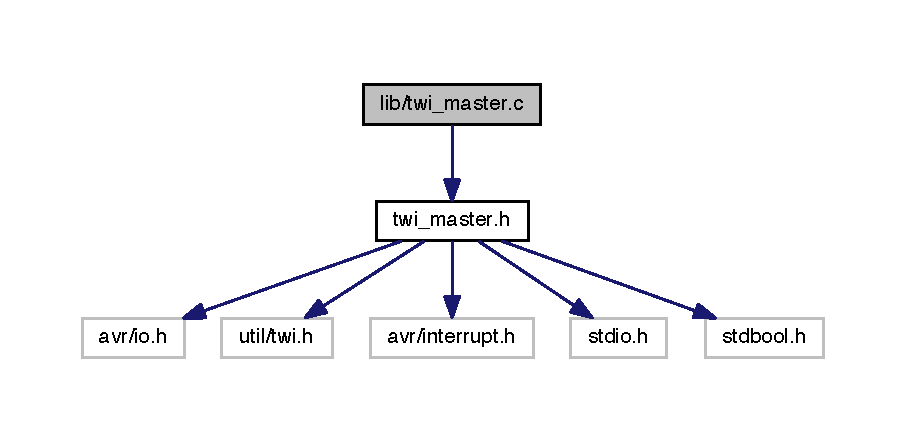
\includegraphics[width=350pt]{twi__master_8c__incl}
\end{center}
\end{figure}
\subsection*{Functions}
\begin{DoxyCompactItemize}
\item 
void \hyperlink{twi__master_8c_ab8b47eb0b53e13c4b34647c2c97388fd}{twi\-\_\-master\-\_\-init} ()
\begin{DoxyCompactList}\small\item\em Setup the twi module. \end{DoxyCompactList}\item 
void \hyperlink{twi__master_8c_a38ff1db93a888454fab7847af2a0f5c7}{twi\-\_\-send\-\_\-data} (uint8\-\_\-t slave, uint8\-\_\-t anz\-\_\-bytes)
\begin{DoxyCompactList}\small\item\em Method to send data to a slave. \end{DoxyCompactList}\item 
void \hyperlink{twi__master_8c_a095a100e547815faf66df46a87968988}{twi\-\_\-receive\-\_\-data} (uint8\-\_\-t slave, uint8\-\_\-t anz\-\_\-bytes)
\begin{DoxyCompactList}\small\item\em Corresponding to send\-\_\-data this method receives data the same way. \end{DoxyCompactList}\item 
void \hyperlink{twi__master_8c_a89bdf8dea79a9e017c3821b6e270c093}{twi\-\_\-master\-\_\-set\-\_\-ready} ()
\item 
\hyperlink{twi__master_8c_a474f42eedbdc093683fdb4b88be3c48f}{I\-S\-R} (T\-W\-I\-\_\-vect)
\begin{DoxyCompactList}\small\item\em This Interrupt Service Routine handles all possible status conditions of the T\-W\-I hardware. \end{DoxyCompactList}\end{DoxyCompactItemize}
\subsection*{Variables}
\begin{DoxyCompactItemize}
\item 
volatile uint8\-\_\-t \hyperlink{twi__master_8c_ae178071b85b716b65d0b856e85534c3b}{twi\-\_\-receive\-\_\-buffer} \mbox{[}\hyperlink{twi__master_8h_a6b20d41d6252e9871430c242cb1a56e7}{B\-U\-F\-F\-E\-R\-\_\-\-S\-I\-Z\-E}\mbox{]}
\item 
volatile uint8\-\_\-t \hyperlink{twi__master_8c_a0ebfdf89c2595f09b88e3fa8d5f3ec3b}{twi\-\_\-send\-\_\-buffer} \mbox{[}\hyperlink{twi__master_8h_a6b20d41d6252e9871430c242cb1a56e7}{B\-U\-F\-F\-E\-R\-\_\-\-S\-I\-Z\-E}\mbox{]}
\item 
volatile uint8\-\_\-t \hyperlink{twi__master_8c_a926e6e50d6c5aca7f59eba912f869ebe}{transmitter}
\item 
volatile uint8\-\_\-t \hyperlink{twi__master_8c_ae92e79ba1068f524ceedbdf8049ef43e}{rindx}
\item 
volatile uint8\-\_\-t \hyperlink{twi__master_8c_ac2f9e24d25da5bfdbeb188d3f09e7619}{sindx}
\item 
volatile uint8\-\_\-t \hyperlink{twi__master_8c_a72a28732edd60c3bdb789466923678a1}{number\-\_\-of\-\_\-bytes}
\item 
volatile uint8\-\_\-t \hyperlink{twi__master_8c_a3dec6baf6b8e19f87fb59089679d3094}{ready}
\item 
volatile uint8\-\_\-t \hyperlink{twi__master_8c_a2611e342f148c60ff2a7a02415541917}{sla}
\end{DoxyCompactItemize}


\subsection{Function Documentation}
\hypertarget{twi__master_8c_a474f42eedbdc093683fdb4b88be3c48f}{\index{twi\-\_\-master.\-c@{twi\-\_\-master.\-c}!I\-S\-R@{I\-S\-R}}
\index{I\-S\-R@{I\-S\-R}!twi_master.c@{twi\-\_\-master.\-c}}
\subsubsection[{I\-S\-R}]{\setlength{\rightskip}{0pt plus 5cm}I\-S\-R (
\begin{DoxyParamCaption}
\item[{T\-W\-I\-\_\-vect}]{}
\end{DoxyParamCaption}
)}}\label{twi__master_8c_a474f42eedbdc093683fdb4b88be3c48f}


This Interrupt Service Routine handles all possible status conditions of the T\-W\-I hardware. 

Everytime a bus operation has finished, the T\-W\-I modules triggers a T\-W\-I interrupt. In this case the \hyperlink{twi__master_8c_a474f42eedbdc093683fdb4b88be3c48f}{I\-S\-R(\-T\-W\-I\-\_\-vect)} is executed. By determing the twi status by reading the T\-W\-S\-R code, we can see in which state of communication we are and take proper actions to continue the transmission.

A more detailed description can be found here\-: isr\-\_\-master 

Definition at line 176 of file twi\-\_\-master.\-c.



References number\-\_\-of\-\_\-bytes, ready, rindx, sindx, sla, transmitter, twi\-\_\-receive\-\_\-buffer, and twi\-\_\-send\-\_\-buffer.

\hypertarget{twi__master_8c_ab8b47eb0b53e13c4b34647c2c97388fd}{\index{twi\-\_\-master.\-c@{twi\-\_\-master.\-c}!twi\-\_\-master\-\_\-init@{twi\-\_\-master\-\_\-init}}
\index{twi\-\_\-master\-\_\-init@{twi\-\_\-master\-\_\-init}!twi_master.c@{twi\-\_\-master.\-c}}
\subsubsection[{twi\-\_\-master\-\_\-init}]{\setlength{\rightskip}{0pt plus 5cm}void twi\-\_\-master\-\_\-init (
\begin{DoxyParamCaption}
{}
\end{DoxyParamCaption}
)}}\label{twi__master_8c_ab8b47eb0b53e13c4b34647c2c97388fd}


Setup the twi module. 

This function sets up the twi module for master operation. Therefore we have to write proper values to the following registers\-:


\begin{DoxyItemize}
\item T\-W\-B\-R Two Wire Bitrate Register
\item T\-W\-S\-R Two Wire Status Register
\item T\-W\-C\-R Two Wire Control Register 
\end{DoxyItemize}

T\-W\-B\-R and T\-W\-S\-R are used to configure the bus clock speed. The T\-W\-I specifications allows us to choose between two different clock speed modes\-: one below 100k\-Hz and one up to 400k\-Hz.\par
 The following equation shows how to set up the clock speed\-:

S\-C\-L frequency = C\-P\-U clock / 16 + 2 $\ast$ T\-W\-B\-R $\ast$ (4 $^\wedge$ T\-W\-P\-S)

According to the equation we choosed T\-W\-B\-R = 18 and T\-W\-S\-R = 1 for 100k\-Hz operations.\par
 
\begin{DoxyCode}
TWBR = \hyperlink{twi__master_8h_abcb6be311da26987e2942ef57aaf3fb8}{TWI\_TWBR\_VALUE\_100};
TWSR &= 0b11111100;
TWSR |= 0x01;
\end{DoxyCode}
\par
 As we can see in this tiny code fragment, the T\-W\-P\-S value is encoded by the two last bits of the T\-W\-S\-R register. 

Definition at line 36 of file twi\-\_\-master.\-c.



References T\-W\-I\-\_\-\-T\-W\-B\-R\-\_\-\-V\-A\-L\-U\-E\-\_\-100.

\hypertarget{twi__master_8c_a89bdf8dea79a9e017c3821b6e270c093}{\index{twi\-\_\-master.\-c@{twi\-\_\-master.\-c}!twi\-\_\-master\-\_\-set\-\_\-ready@{twi\-\_\-master\-\_\-set\-\_\-ready}}
\index{twi\-\_\-master\-\_\-set\-\_\-ready@{twi\-\_\-master\-\_\-set\-\_\-ready}!twi_master.c@{twi\-\_\-master.\-c}}
\subsubsection[{twi\-\_\-master\-\_\-set\-\_\-ready}]{\setlength{\rightskip}{0pt plus 5cm}void twi\-\_\-master\-\_\-set\-\_\-ready (
\begin{DoxyParamCaption}
{}
\end{DoxyParamCaption}
)}}\label{twi__master_8c_a89bdf8dea79a9e017c3821b6e270c093}


Definition at line 162 of file twi\-\_\-master.\-c.



References ready.



Referenced by bma020\-\_\-read\-\_\-raw\-\_\-acceleration().

\hypertarget{twi__master_8c_a095a100e547815faf66df46a87968988}{\index{twi\-\_\-master.\-c@{twi\-\_\-master.\-c}!twi\-\_\-receive\-\_\-data@{twi\-\_\-receive\-\_\-data}}
\index{twi\-\_\-receive\-\_\-data@{twi\-\_\-receive\-\_\-data}!twi_master.c@{twi\-\_\-master.\-c}}
\subsubsection[{twi\-\_\-receive\-\_\-data}]{\setlength{\rightskip}{0pt plus 5cm}void twi\-\_\-receive\-\_\-data (
\begin{DoxyParamCaption}
\item[{uint8\-\_\-t}]{slave, }
\item[{uint8\-\_\-t}]{anz\-\_\-bytes}
\end{DoxyParamCaption}
)}}\label{twi__master_8c_a095a100e547815faf66df46a87968988}


Corresponding to send\-\_\-data this method receives data the same way. 


\begin{DoxyParams}{Parameters}
{\em slave} & contains the slave adress \\
\hline
{\em anz\-\_\-bytes} & contains the amount of bytes that have to be transmitted\\
\hline
\end{DoxyParams}
A global receive\-\_\-buffer is used to store data that is received by T\-W\-I. 
\begin{DoxyCode}
\textcolor{keyword}{extern} \textcolor{keywordtype}{void} receive\_data(uint8\_t slave, uint8\_t anz\_bytes)
\{
    \hyperlink{twi__master_8c_a3dec6baf6b8e19f87fb59089679d3094}{ready} = FALSE;
    \hyperlink{twi__master_8c_a926e6e50d6c5aca7f59eba912f869ebe}{transmitter} = FALSE;
    \hyperlink{twi__master_8c_a2611e342f148c60ff2a7a02415541917}{sla} = slave;
    \hyperlink{twi__master_8c_a72a28732edd60c3bdb789466923678a1}{number\_of\_bytes} = anz\_bytes;
    \hyperlink{twi__master_8c_ae92e79ba1068f524ceedbdf8049ef43e}{rindx} = 0;
    TWCR = (1<<TWINT) | (1<<TWSTA) | (1<<TWEN) | (1<<TWIE);
    \textcolor{keywordflow}{while}(!\hyperlink{twi__master_8c_a3dec6baf6b8e19f87fb59089679d3094}{ready})\{\}
\}
\end{DoxyCode}
 The only differences\-: \par
{\bfseries transmitter} is set to F\-A\-L\-S\-E \par
Instead of sindex we set rindex to zero. 

Definition at line 151 of file twi\-\_\-master.\-c.



References number\-\_\-of\-\_\-bytes, ready, rindx, sla, and transmitter.



Referenced by bma020\-\_\-read\-\_\-raw\-\_\-acceleration().

\hypertarget{twi__master_8c_a38ff1db93a888454fab7847af2a0f5c7}{\index{twi\-\_\-master.\-c@{twi\-\_\-master.\-c}!twi\-\_\-send\-\_\-data@{twi\-\_\-send\-\_\-data}}
\index{twi\-\_\-send\-\_\-data@{twi\-\_\-send\-\_\-data}!twi_master.c@{twi\-\_\-master.\-c}}
\subsubsection[{twi\-\_\-send\-\_\-data}]{\setlength{\rightskip}{0pt plus 5cm}void twi\-\_\-send\-\_\-data (
\begin{DoxyParamCaption}
\item[{uint8\-\_\-t}]{slave, }
\item[{uint8\-\_\-t}]{anz\-\_\-bytes}
\end{DoxyParamCaption}
)}}\label{twi__master_8c_a38ff1db93a888454fab7847af2a0f5c7}


Method to send data to a slave. 


\begin{DoxyParams}{Parameters}
{\em slave} & contains the slave adress \\
\hline
{\em anz\-\_\-bytes} & contains the amount of bytes that have to be transmitted\\
\hline
\end{DoxyParams}
The data to be transmitted is stored in the global variable send\-\_\-buffer. send\-\_\-buffer\mbox{[}\mbox{]} is an array of uint8\-\_\-t types. It's size is defined by the constant B\-U\-F\-\_\-\-S\-I\-Z\-E. The declaration of send\-\_\-buffer is located in the \hyperlink{twi__master_8h}{twi\-\_\-master.\-h} file. 

If one wants to transmit data to a slave, he has to write the data to the send\-\_\-buffer. After calling the send\-\_\-data() method, all bytes from send\-\_\-buffer\mbox{[}0\mbox{]} to send\-\_\-buffer\mbox{[}anz\-\_\-bytes -\/ 1\mbox{]} will be transmitted to the slave without interruption.


\begin{DoxyCode}
\textcolor{keyword}{extern} \textcolor{keywordtype}{void} send\_data(uint8\_t slave, uint8\_t anz\_bytes)
\{
    \hyperlink{twi__master_8c_a3dec6baf6b8e19f87fb59089679d3094}{ready} = \textcolor{keyword}{false};
    \hyperlink{twi__master_8c_a926e6e50d6c5aca7f59eba912f869ebe}{transmitter} = \textcolor{keyword}{true};
    \hyperlink{twi__master_8c_a2611e342f148c60ff2a7a02415541917}{sla} = slave;
    \hyperlink{twi__master_8c_a72a28732edd60c3bdb789466923678a1}{number\_of\_bytes} = anz\_bytes;
    \hyperlink{twi__master_8c_ac2f9e24d25da5bfdbeb188d3f09e7619}{sindx} = 0;
    TWCR = (1<<TWINT) | (1<<TWSTA) | (1<<TWEN) | (1<<TWIE);
    \textcolor{keywordflow}{while}(!\hyperlink{twi__master_8c_a3dec6baf6b8e19f87fb59089679d3094}{ready})\{\}
\}
\end{DoxyCode}
 Code explanation in detail\-: 


\begin{DoxyCode}
\hyperlink{twi__master_8c_a3dec6baf6b8e19f87fb59089679d3094}{ready} = \textcolor{keyword}{false};
\end{DoxyCode}
 The {\bfseries ready} variable is used to guarantee, that the whole transmission of every bytes is done without interruption. The program flow within the main method of this master controller is halted until all bytes have been transmitted. 


\begin{DoxyCode}
\hyperlink{twi__master_8c_a926e6e50d6c5aca7f59eba912f869ebe}{transmitter} = \textcolor{keyword}{true};
\end{DoxyCode}
 By setting the variable {\bfseries transmitter} to {\itshape T\-R\-U\-E}, the I\-S\-R of the master controller can determine wether Master Transmitter or Master Receiver mode is active. 


\begin{DoxyCode}
\hyperlink{twi__master_8c_a2611e342f148c60ff2a7a02415541917}{sla} = slave;
\end{DoxyCode}
 Store the slave adress in the global variable sla to make it visible for the I\-S\-R. Same with anz\-\_\-bytes. 


\begin{DoxyCode}
\hyperlink{twi__master_8c_ac2f9e24d25da5bfdbeb188d3f09e7619}{sindx} = 0;
\end{DoxyCode}
 Set the send\-\_\-buffer index to zero. 


\begin{DoxyCode}
TWCR = (1<<TWINT) | (1<<TWSTA) | (1<<TWEN) | (1<<TWIE);
\end{DoxyCode}
 Here we can see how to manipulate the Two Wire Control Register. \par
T\-W\-I\-N\-T causes the T\-W\-I to trigger an interrupt so that the I\-S\-R executes. \par
T\-W\-S\-T\-A cause the T\-W\-I to put a {\itshape  start signal } on the T\-W\-I bus. All attached slave will recognize the start signal. \par
T\-W\-E\-N enables the T\-W\-I. \par
T\-W\-I\-E Two Wire Interrupt Enable allows the T\-W\-I to trigger interrupts. 


\begin{DoxyCode}
\textcolor{keywordflow}{while}(!\hyperlink{twi__master_8c_a3dec6baf6b8e19f87fb59089679d3094}{ready})\{\}
The \hyperlink{twi__master_8c_a3dec6baf6b8e19f87fb59089679d3094}{ready} flag is set within the \hyperlink{twi__master_8c_a474f42eedbdc093683fdb4b88be3c48f}{ISR} when the TWI reaches an end state that indicates that the 
      transmission
has finished.
\end{DoxyCode}
 

Definition at line 115 of file twi\-\_\-master.\-c.



References number\-\_\-of\-\_\-bytes, ready, sindx, sla, and transmitter.



Referenced by bma020\-\_\-read\-\_\-raw\-\_\-acceleration().



\subsection{Variable Documentation}
\hypertarget{twi__master_8c_a72a28732edd60c3bdb789466923678a1}{\index{twi\-\_\-master.\-c@{twi\-\_\-master.\-c}!number\-\_\-of\-\_\-bytes@{number\-\_\-of\-\_\-bytes}}
\index{number\-\_\-of\-\_\-bytes@{number\-\_\-of\-\_\-bytes}!twi_master.c@{twi\-\_\-master.\-c}}
\subsubsection[{number\-\_\-of\-\_\-bytes}]{\setlength{\rightskip}{0pt plus 5cm}volatile uint8\-\_\-t number\-\_\-of\-\_\-bytes}}\label{twi__master_8c_a72a28732edd60c3bdb789466923678a1}


Definition at line 12 of file twi\-\_\-master.\-c.



Referenced by I\-S\-R(), twi\-\_\-receive\-\_\-data(), and twi\-\_\-send\-\_\-data().

\hypertarget{twi__master_8c_a3dec6baf6b8e19f87fb59089679d3094}{\index{twi\-\_\-master.\-c@{twi\-\_\-master.\-c}!ready@{ready}}
\index{ready@{ready}!twi_master.c@{twi\-\_\-master.\-c}}
\subsubsection[{ready}]{\setlength{\rightskip}{0pt plus 5cm}volatile uint8\-\_\-t ready}}\label{twi__master_8c_a3dec6baf6b8e19f87fb59089679d3094}


Definition at line 13 of file twi\-\_\-master.\-c.



Referenced by I\-S\-R(), twi\-\_\-master\-\_\-set\-\_\-ready(), twi\-\_\-receive\-\_\-data(), and twi\-\_\-send\-\_\-data().

\hypertarget{twi__master_8c_ae92e79ba1068f524ceedbdf8049ef43e}{\index{twi\-\_\-master.\-c@{twi\-\_\-master.\-c}!rindx@{rindx}}
\index{rindx@{rindx}!twi_master.c@{twi\-\_\-master.\-c}}
\subsubsection[{rindx}]{\setlength{\rightskip}{0pt plus 5cm}volatile uint8\-\_\-t rindx}}\label{twi__master_8c_ae92e79ba1068f524ceedbdf8049ef43e}


Definition at line 10 of file twi\-\_\-master.\-c.



Referenced by I\-S\-R(), and twi\-\_\-receive\-\_\-data().

\hypertarget{twi__master_8c_ac2f9e24d25da5bfdbeb188d3f09e7619}{\index{twi\-\_\-master.\-c@{twi\-\_\-master.\-c}!sindx@{sindx}}
\index{sindx@{sindx}!twi_master.c@{twi\-\_\-master.\-c}}
\subsubsection[{sindx}]{\setlength{\rightskip}{0pt plus 5cm}volatile uint8\-\_\-t sindx}}\label{twi__master_8c_ac2f9e24d25da5bfdbeb188d3f09e7619}


Definition at line 11 of file twi\-\_\-master.\-c.



Referenced by I\-S\-R(), and twi\-\_\-send\-\_\-data().

\hypertarget{twi__master_8c_a2611e342f148c60ff2a7a02415541917}{\index{twi\-\_\-master.\-c@{twi\-\_\-master.\-c}!sla@{sla}}
\index{sla@{sla}!twi_master.c@{twi\-\_\-master.\-c}}
\subsubsection[{sla}]{\setlength{\rightskip}{0pt plus 5cm}volatile uint8\-\_\-t sla}}\label{twi__master_8c_a2611e342f148c60ff2a7a02415541917}


Definition at line 14 of file twi\-\_\-master.\-c.



Referenced by I\-S\-R(), twi\-\_\-receive\-\_\-data(), and twi\-\_\-send\-\_\-data().

\hypertarget{twi__master_8c_a926e6e50d6c5aca7f59eba912f869ebe}{\index{twi\-\_\-master.\-c@{twi\-\_\-master.\-c}!transmitter@{transmitter}}
\index{transmitter@{transmitter}!twi_master.c@{twi\-\_\-master.\-c}}
\subsubsection[{transmitter}]{\setlength{\rightskip}{0pt plus 5cm}volatile uint8\-\_\-t transmitter}}\label{twi__master_8c_a926e6e50d6c5aca7f59eba912f869ebe}


Definition at line 9 of file twi\-\_\-master.\-c.



Referenced by I\-S\-R(), twi\-\_\-receive\-\_\-data(), and twi\-\_\-send\-\_\-data().

\hypertarget{twi__master_8c_ae178071b85b716b65d0b856e85534c3b}{\index{twi\-\_\-master.\-c@{twi\-\_\-master.\-c}!twi\-\_\-receive\-\_\-buffer@{twi\-\_\-receive\-\_\-buffer}}
\index{twi\-\_\-receive\-\_\-buffer@{twi\-\_\-receive\-\_\-buffer}!twi_master.c@{twi\-\_\-master.\-c}}
\subsubsection[{twi\-\_\-receive\-\_\-buffer}]{\setlength{\rightskip}{0pt plus 5cm}volatile uint8\-\_\-t twi\-\_\-receive\-\_\-buffer\mbox{[}{\bf B\-U\-F\-F\-E\-R\-\_\-\-S\-I\-Z\-E}\mbox{]}}}\label{twi__master_8c_ae178071b85b716b65d0b856e85534c3b}


Definition at line 5 of file twi\-\_\-master.\-c.



Referenced by bma020\-\_\-read\-\_\-raw\-\_\-acceleration(), and I\-S\-R().

\hypertarget{twi__master_8c_a0ebfdf89c2595f09b88e3fa8d5f3ec3b}{\index{twi\-\_\-master.\-c@{twi\-\_\-master.\-c}!twi\-\_\-send\-\_\-buffer@{twi\-\_\-send\-\_\-buffer}}
\index{twi\-\_\-send\-\_\-buffer@{twi\-\_\-send\-\_\-buffer}!twi_master.c@{twi\-\_\-master.\-c}}
\subsubsection[{twi\-\_\-send\-\_\-buffer}]{\setlength{\rightskip}{0pt plus 5cm}volatile uint8\-\_\-t twi\-\_\-send\-\_\-buffer\mbox{[}{\bf B\-U\-F\-F\-E\-R\-\_\-\-S\-I\-Z\-E}\mbox{]}}}\label{twi__master_8c_a0ebfdf89c2595f09b88e3fa8d5f3ec3b}


Definition at line 6 of file twi\-\_\-master.\-c.



Referenced by bma020\-\_\-read\-\_\-raw\-\_\-acceleration(), and I\-S\-R().


\hypertarget{twi__master_8h}{\section{lib/twi\-\_\-master.h File Reference}
\label{twi__master_8h}\index{lib/twi\-\_\-master.\-h@{lib/twi\-\_\-master.\-h}}
}
{\ttfamily \#include $<$avr/io.\-h$>$}\\*
{\ttfamily \#include $<$util/twi.\-h$>$}\\*
{\ttfamily \#include $<$avr/interrupt.\-h$>$}\\*
{\ttfamily \#include $<$stdio.\-h$>$}\\*
{\ttfamily \#include $<$stdbool.\-h$>$}\\*
Include dependency graph for twi\-\_\-master.\-h\-:\nopagebreak
\begin{figure}[H]
\begin{center}
\leavevmode
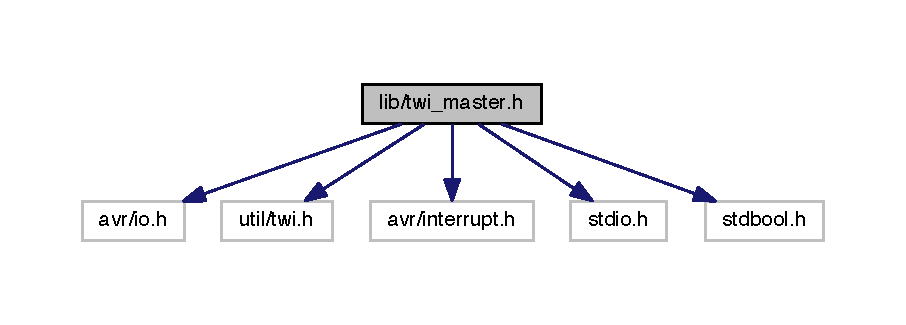
\includegraphics[width=350pt]{twi__master_8h__incl}
\end{center}
\end{figure}
This graph shows which files directly or indirectly include this file\-:\nopagebreak
\begin{figure}[H]
\begin{center}
\leavevmode
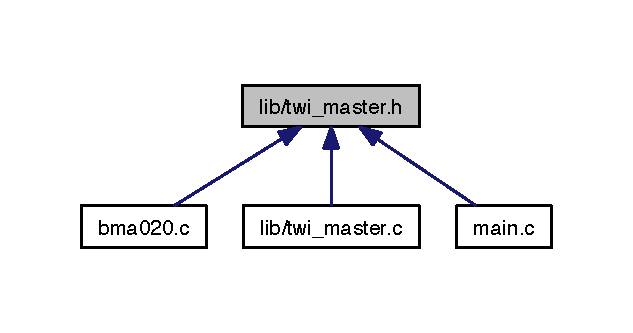
\includegraphics[width=304pt]{twi__master_8h__dep__incl}
\end{center}
\end{figure}
\subsection*{Macros}
\begin{DoxyCompactItemize}
\item 
\#define \hyperlink{twi__master_8h_a22a867687aab643bc7819b2859949015}{T\-W\-I\-\_\-\-T\-W\-B\-R\-\_\-\-V\-A\-L\-U\-E\-\_\-400}~3
\item 
\#define \hyperlink{twi__master_8h_abcb6be311da26987e2942ef57aaf3fb8}{T\-W\-I\-\_\-\-T\-W\-B\-R\-\_\-\-V\-A\-L\-U\-E\-\_\-100}~18
\item 
\#define \hyperlink{twi__master_8h_a60d57424619b46be2be903cb8a0c2180}{T\-W\-I\-\_\-\-T\-W\-B\-R\-\_\-\-V\-A\-L\-U\-E\-\_\-25}~78
\item 
\#define \hyperlink{twi__master_8h_a056482c8c7b67601021519afe041d1aa}{T\-W\-I\-\_\-\-T\-W\-P\-S\-\_\-\-V\-A\-L\-U\-E}~1
\item 
\#define \hyperlink{twi__master_8h_a6b20d41d6252e9871430c242cb1a56e7}{B\-U\-F\-F\-E\-R\-\_\-\-S\-I\-Z\-E}~10
\end{DoxyCompactItemize}
\subsection*{Functions}
\begin{DoxyCompactItemize}
\item 
void \hyperlink{twi__master_8h_ab8b47eb0b53e13c4b34647c2c97388fd}{twi\-\_\-master\-\_\-init} ()
\begin{DoxyCompactList}\small\item\em Setup the twi module. \end{DoxyCompactList}\item 
void \hyperlink{twi__master_8h_a38ff1db93a888454fab7847af2a0f5c7}{twi\-\_\-send\-\_\-data} (uint8\-\_\-t slave, uint8\-\_\-t anz\-\_\-bytes)
\begin{DoxyCompactList}\small\item\em Method to send data to a slave. \end{DoxyCompactList}\item 
void \hyperlink{twi__master_8h_a095a100e547815faf66df46a87968988}{twi\-\_\-receive\-\_\-data} (uint8\-\_\-t slave, uint8\-\_\-t anz\-\_\-bytes)
\begin{DoxyCompactList}\small\item\em Corresponding to send\-\_\-data this method receives data the same way. \end{DoxyCompactList}\item 
void \hyperlink{twi__master_8h_a89bdf8dea79a9e017c3821b6e270c093}{twi\-\_\-master\-\_\-set\-\_\-ready} ()
\end{DoxyCompactItemize}
\subsection*{Variables}
\begin{DoxyCompactItemize}
\item 
volatile uint8\-\_\-t \hyperlink{twi__master_8h_ae178071b85b716b65d0b856e85534c3b}{twi\-\_\-receive\-\_\-buffer} \mbox{[}\hyperlink{twi__master_8h_a6b20d41d6252e9871430c242cb1a56e7}{B\-U\-F\-F\-E\-R\-\_\-\-S\-I\-Z\-E}\mbox{]}
\item 
volatile uint8\-\_\-t \hyperlink{twi__master_8h_a0ebfdf89c2595f09b88e3fa8d5f3ec3b}{twi\-\_\-send\-\_\-buffer} \mbox{[}\hyperlink{twi__master_8h_a6b20d41d6252e9871430c242cb1a56e7}{B\-U\-F\-F\-E\-R\-\_\-\-S\-I\-Z\-E}\mbox{]}
\end{DoxyCompactItemize}


\subsection{Macro Definition Documentation}
\hypertarget{twi__master_8h_a6b20d41d6252e9871430c242cb1a56e7}{\index{twi\-\_\-master.\-h@{twi\-\_\-master.\-h}!B\-U\-F\-F\-E\-R\-\_\-\-S\-I\-Z\-E@{B\-U\-F\-F\-E\-R\-\_\-\-S\-I\-Z\-E}}
\index{B\-U\-F\-F\-E\-R\-\_\-\-S\-I\-Z\-E@{B\-U\-F\-F\-E\-R\-\_\-\-S\-I\-Z\-E}!twi_master.h@{twi\-\_\-master.\-h}}
\subsubsection[{B\-U\-F\-F\-E\-R\-\_\-\-S\-I\-Z\-E}]{\setlength{\rightskip}{0pt plus 5cm}\#define B\-U\-F\-F\-E\-R\-\_\-\-S\-I\-Z\-E~10}}\label{twi__master_8h_a6b20d41d6252e9871430c242cb1a56e7}


Definition at line 10 of file twi\-\_\-master.\-h.

\hypertarget{twi__master_8h_abcb6be311da26987e2942ef57aaf3fb8}{\index{twi\-\_\-master.\-h@{twi\-\_\-master.\-h}!T\-W\-I\-\_\-\-T\-W\-B\-R\-\_\-\-V\-A\-L\-U\-E\-\_\-100@{T\-W\-I\-\_\-\-T\-W\-B\-R\-\_\-\-V\-A\-L\-U\-E\-\_\-100}}
\index{T\-W\-I\-\_\-\-T\-W\-B\-R\-\_\-\-V\-A\-L\-U\-E\-\_\-100@{T\-W\-I\-\_\-\-T\-W\-B\-R\-\_\-\-V\-A\-L\-U\-E\-\_\-100}!twi_master.h@{twi\-\_\-master.\-h}}
\subsubsection[{T\-W\-I\-\_\-\-T\-W\-B\-R\-\_\-\-V\-A\-L\-U\-E\-\_\-100}]{\setlength{\rightskip}{0pt plus 5cm}\#define T\-W\-I\-\_\-\-T\-W\-B\-R\-\_\-\-V\-A\-L\-U\-E\-\_\-100~18}}\label{twi__master_8h_abcb6be311da26987e2942ef57aaf3fb8}
Defines the T\-W\-B\-R value for 100 k\-Hz T\-W\-I operation 

Definition at line 2 of file twi\-\_\-master.\-h.



Referenced by twi\-\_\-master\-\_\-init().

\hypertarget{twi__master_8h_a60d57424619b46be2be903cb8a0c2180}{\index{twi\-\_\-master.\-h@{twi\-\_\-master.\-h}!T\-W\-I\-\_\-\-T\-W\-B\-R\-\_\-\-V\-A\-L\-U\-E\-\_\-25@{T\-W\-I\-\_\-\-T\-W\-B\-R\-\_\-\-V\-A\-L\-U\-E\-\_\-25}}
\index{T\-W\-I\-\_\-\-T\-W\-B\-R\-\_\-\-V\-A\-L\-U\-E\-\_\-25@{T\-W\-I\-\_\-\-T\-W\-B\-R\-\_\-\-V\-A\-L\-U\-E\-\_\-25}!twi_master.h@{twi\-\_\-master.\-h}}
\subsubsection[{T\-W\-I\-\_\-\-T\-W\-B\-R\-\_\-\-V\-A\-L\-U\-E\-\_\-25}]{\setlength{\rightskip}{0pt plus 5cm}\#define T\-W\-I\-\_\-\-T\-W\-B\-R\-\_\-\-V\-A\-L\-U\-E\-\_\-25~78}}\label{twi__master_8h_a60d57424619b46be2be903cb8a0c2180}


Definition at line 3 of file twi\-\_\-master.\-h.

\hypertarget{twi__master_8h_a22a867687aab643bc7819b2859949015}{\index{twi\-\_\-master.\-h@{twi\-\_\-master.\-h}!T\-W\-I\-\_\-\-T\-W\-B\-R\-\_\-\-V\-A\-L\-U\-E\-\_\-400@{T\-W\-I\-\_\-\-T\-W\-B\-R\-\_\-\-V\-A\-L\-U\-E\-\_\-400}}
\index{T\-W\-I\-\_\-\-T\-W\-B\-R\-\_\-\-V\-A\-L\-U\-E\-\_\-400@{T\-W\-I\-\_\-\-T\-W\-B\-R\-\_\-\-V\-A\-L\-U\-E\-\_\-400}!twi_master.h@{twi\-\_\-master.\-h}}
\subsubsection[{T\-W\-I\-\_\-\-T\-W\-B\-R\-\_\-\-V\-A\-L\-U\-E\-\_\-400}]{\setlength{\rightskip}{0pt plus 5cm}\#define T\-W\-I\-\_\-\-T\-W\-B\-R\-\_\-\-V\-A\-L\-U\-E\-\_\-400~3}}\label{twi__master_8h_a22a867687aab643bc7819b2859949015}
Defines the T\-W\-B\-R value for 400 k\-Hz T\-W\-I operation 

Definition at line 1 of file twi\-\_\-master.\-h.

\hypertarget{twi__master_8h_a056482c8c7b67601021519afe041d1aa}{\index{twi\-\_\-master.\-h@{twi\-\_\-master.\-h}!T\-W\-I\-\_\-\-T\-W\-P\-S\-\_\-\-V\-A\-L\-U\-E@{T\-W\-I\-\_\-\-T\-W\-P\-S\-\_\-\-V\-A\-L\-U\-E}}
\index{T\-W\-I\-\_\-\-T\-W\-P\-S\-\_\-\-V\-A\-L\-U\-E@{T\-W\-I\-\_\-\-T\-W\-P\-S\-\_\-\-V\-A\-L\-U\-E}!twi_master.h@{twi\-\_\-master.\-h}}
\subsubsection[{T\-W\-I\-\_\-\-T\-W\-P\-S\-\_\-\-V\-A\-L\-U\-E}]{\setlength{\rightskip}{0pt plus 5cm}\#define T\-W\-I\-\_\-\-T\-W\-P\-S\-\_\-\-V\-A\-L\-U\-E~1}}\label{twi__master_8h_a056482c8c7b67601021519afe041d1aa}
The prescaler is always 1 correspondig to the following equation\-:\par
 S\-C\-L frequency = C\-P\-U clock / 16 + 2 $\ast$ T\-W\-B\-R $\ast$ (4 $^\wedge$ T\-W\-P\-S) 

Definition at line 4 of file twi\-\_\-master.\-h.



\subsection{Function Documentation}
\hypertarget{twi__master_8h_ab8b47eb0b53e13c4b34647c2c97388fd}{\index{twi\-\_\-master.\-h@{twi\-\_\-master.\-h}!twi\-\_\-master\-\_\-init@{twi\-\_\-master\-\_\-init}}
\index{twi\-\_\-master\-\_\-init@{twi\-\_\-master\-\_\-init}!twi_master.h@{twi\-\_\-master.\-h}}
\subsubsection[{twi\-\_\-master\-\_\-init}]{\setlength{\rightskip}{0pt plus 5cm}void twi\-\_\-master\-\_\-init (
\begin{DoxyParamCaption}
{}
\end{DoxyParamCaption}
)}}\label{twi__master_8h_ab8b47eb0b53e13c4b34647c2c97388fd}


Setup the twi module. 

This function sets up the twi module for master operation. Therefore we have to write proper values to the following registers\-:


\begin{DoxyItemize}
\item T\-W\-B\-R Two Wire Bitrate Register
\item T\-W\-S\-R Two Wire Status Register
\item T\-W\-C\-R Two Wire Control Register 
\end{DoxyItemize}

T\-W\-B\-R and T\-W\-S\-R are used to configure the bus clock speed. The T\-W\-I specifications allows us to choose between two different clock speed modes\-: one below 100k\-Hz and one up to 400k\-Hz.\par
 The following equation shows how to set up the clock speed\-:

S\-C\-L frequency = C\-P\-U clock / 16 + 2 $\ast$ T\-W\-B\-R $\ast$ (4 $^\wedge$ T\-W\-P\-S)

According to the equation we choosed T\-W\-B\-R = 18 and T\-W\-S\-R = 1 for 100k\-Hz operations.\par
 
\begin{DoxyCode}
TWBR = \hyperlink{twi__master_8h_abcb6be311da26987e2942ef57aaf3fb8}{TWI\_TWBR\_VALUE\_100};
TWSR &= 0b11111100;
TWSR |= 0x01;
\end{DoxyCode}
\par
 As we can see in this tiny code fragment, the T\-W\-P\-S value is encoded by the two last bits of the T\-W\-S\-R register. 

Definition at line 36 of file twi\-\_\-master.\-c.



References T\-W\-I\-\_\-\-T\-W\-B\-R\-\_\-\-V\-A\-L\-U\-E\-\_\-100.

\hypertarget{twi__master_8h_a89bdf8dea79a9e017c3821b6e270c093}{\index{twi\-\_\-master.\-h@{twi\-\_\-master.\-h}!twi\-\_\-master\-\_\-set\-\_\-ready@{twi\-\_\-master\-\_\-set\-\_\-ready}}
\index{twi\-\_\-master\-\_\-set\-\_\-ready@{twi\-\_\-master\-\_\-set\-\_\-ready}!twi_master.h@{twi\-\_\-master.\-h}}
\subsubsection[{twi\-\_\-master\-\_\-set\-\_\-ready}]{\setlength{\rightskip}{0pt plus 5cm}void twi\-\_\-master\-\_\-set\-\_\-ready (
\begin{DoxyParamCaption}
{}
\end{DoxyParamCaption}
)}}\label{twi__master_8h_a89bdf8dea79a9e017c3821b6e270c093}


Definition at line 162 of file twi\-\_\-master.\-c.



References ready.



Referenced by bma020\-\_\-read\-\_\-raw\-\_\-acceleration().

\hypertarget{twi__master_8h_a095a100e547815faf66df46a87968988}{\index{twi\-\_\-master.\-h@{twi\-\_\-master.\-h}!twi\-\_\-receive\-\_\-data@{twi\-\_\-receive\-\_\-data}}
\index{twi\-\_\-receive\-\_\-data@{twi\-\_\-receive\-\_\-data}!twi_master.h@{twi\-\_\-master.\-h}}
\subsubsection[{twi\-\_\-receive\-\_\-data}]{\setlength{\rightskip}{0pt plus 5cm}void twi\-\_\-receive\-\_\-data (
\begin{DoxyParamCaption}
\item[{uint8\-\_\-t}]{slave, }
\item[{uint8\-\_\-t}]{anz\-\_\-bytes}
\end{DoxyParamCaption}
)}}\label{twi__master_8h_a095a100e547815faf66df46a87968988}


Corresponding to send\-\_\-data this method receives data the same way. 


\begin{DoxyParams}{Parameters}
{\em slave} & contains the slave adress \\
\hline
{\em anz\-\_\-bytes} & contains the amount of bytes that have to be transmitted\\
\hline
\end{DoxyParams}
A global receive\-\_\-buffer is used to store data that is received by T\-W\-I. 
\begin{DoxyCode}
\textcolor{keyword}{extern} \textcolor{keywordtype}{void} receive\_data(uint8\_t slave, uint8\_t anz\_bytes)
\{
    \hyperlink{twi__master_8c_a3dec6baf6b8e19f87fb59089679d3094}{ready} = FALSE;
    \hyperlink{twi__master_8c_a926e6e50d6c5aca7f59eba912f869ebe}{transmitter} = FALSE;
    \hyperlink{twi__master_8c_a2611e342f148c60ff2a7a02415541917}{sla} = slave;
    \hyperlink{twi__master_8c_a72a28732edd60c3bdb789466923678a1}{number\_of\_bytes} = anz\_bytes;
    \hyperlink{twi__master_8c_ae92e79ba1068f524ceedbdf8049ef43e}{rindx} = 0;
    TWCR = (1<<TWINT) | (1<<TWSTA) | (1<<TWEN) | (1<<TWIE);
    \textcolor{keywordflow}{while}(!\hyperlink{twi__master_8c_a3dec6baf6b8e19f87fb59089679d3094}{ready})\{\}
\}
\end{DoxyCode}
 The only differences\-: \par
{\bfseries transmitter} is set to F\-A\-L\-S\-E \par
Instead of sindex we set rindex to zero. 

Definition at line 151 of file twi\-\_\-master.\-c.



References number\-\_\-of\-\_\-bytes, ready, rindx, sla, and transmitter.



Referenced by bma020\-\_\-read\-\_\-raw\-\_\-acceleration().

\hypertarget{twi__master_8h_a38ff1db93a888454fab7847af2a0f5c7}{\index{twi\-\_\-master.\-h@{twi\-\_\-master.\-h}!twi\-\_\-send\-\_\-data@{twi\-\_\-send\-\_\-data}}
\index{twi\-\_\-send\-\_\-data@{twi\-\_\-send\-\_\-data}!twi_master.h@{twi\-\_\-master.\-h}}
\subsubsection[{twi\-\_\-send\-\_\-data}]{\setlength{\rightskip}{0pt plus 5cm}void twi\-\_\-send\-\_\-data (
\begin{DoxyParamCaption}
\item[{uint8\-\_\-t}]{slave, }
\item[{uint8\-\_\-t}]{anz\-\_\-bytes}
\end{DoxyParamCaption}
)}}\label{twi__master_8h_a38ff1db93a888454fab7847af2a0f5c7}


Method to send data to a slave. 


\begin{DoxyParams}{Parameters}
{\em slave} & contains the slave adress \\
\hline
{\em anz\-\_\-bytes} & contains the amount of bytes that have to be transmitted\\
\hline
\end{DoxyParams}
The data to be transmitted is stored in the global variable send\-\_\-buffer. send\-\_\-buffer\mbox{[}\mbox{]} is an array of uint8\-\_\-t types. It's size is defined by the constant B\-U\-F\-\_\-\-S\-I\-Z\-E. The declaration of send\-\_\-buffer is located in the \hyperlink{twi__master_8h}{twi\-\_\-master.\-h} file. 

If one wants to transmit data to a slave, he has to write the data to the send\-\_\-buffer. After calling the send\-\_\-data() method, all bytes from send\-\_\-buffer\mbox{[}0\mbox{]} to send\-\_\-buffer\mbox{[}anz\-\_\-bytes -\/ 1\mbox{]} will be transmitted to the slave without interruption.


\begin{DoxyCode}
\textcolor{keyword}{extern} \textcolor{keywordtype}{void} send\_data(uint8\_t slave, uint8\_t anz\_bytes)
\{
    \hyperlink{twi__master_8c_a3dec6baf6b8e19f87fb59089679d3094}{ready} = \textcolor{keyword}{false};
    \hyperlink{twi__master_8c_a926e6e50d6c5aca7f59eba912f869ebe}{transmitter} = \textcolor{keyword}{true};
    \hyperlink{twi__master_8c_a2611e342f148c60ff2a7a02415541917}{sla} = slave;
    \hyperlink{twi__master_8c_a72a28732edd60c3bdb789466923678a1}{number\_of\_bytes} = anz\_bytes;
    \hyperlink{twi__master_8c_ac2f9e24d25da5bfdbeb188d3f09e7619}{sindx} = 0;
    TWCR = (1<<TWINT) | (1<<TWSTA) | (1<<TWEN) | (1<<TWIE);
    \textcolor{keywordflow}{while}(!\hyperlink{twi__master_8c_a3dec6baf6b8e19f87fb59089679d3094}{ready})\{\}
\}
\end{DoxyCode}
 Code explanation in detail\-: 


\begin{DoxyCode}
\hyperlink{twi__master_8c_a3dec6baf6b8e19f87fb59089679d3094}{ready} = \textcolor{keyword}{false};
\end{DoxyCode}
 The {\bfseries ready} variable is used to guarantee, that the whole transmission of every bytes is done without interruption. The program flow within the main method of this master controller is halted until all bytes have been transmitted. 


\begin{DoxyCode}
\hyperlink{twi__master_8c_a926e6e50d6c5aca7f59eba912f869ebe}{transmitter} = \textcolor{keyword}{true};
\end{DoxyCode}
 By setting the variable {\bfseries transmitter} to {\itshape T\-R\-U\-E}, the I\-S\-R of the master controller can determine wether Master Transmitter or Master Receiver mode is active. 


\begin{DoxyCode}
\hyperlink{twi__master_8c_a2611e342f148c60ff2a7a02415541917}{sla} = slave;
\end{DoxyCode}
 Store the slave adress in the global variable sla to make it visible for the I\-S\-R. Same with anz\-\_\-bytes. 


\begin{DoxyCode}
\hyperlink{twi__master_8c_ac2f9e24d25da5bfdbeb188d3f09e7619}{sindx} = 0;
\end{DoxyCode}
 Set the send\-\_\-buffer index to zero. 


\begin{DoxyCode}
TWCR = (1<<TWINT) | (1<<TWSTA) | (1<<TWEN) | (1<<TWIE);
\end{DoxyCode}
 Here we can see how to manipulate the Two Wire Control Register. \par
T\-W\-I\-N\-T causes the T\-W\-I to trigger an interrupt so that the I\-S\-R executes. \par
T\-W\-S\-T\-A cause the T\-W\-I to put a {\itshape  start signal } on the T\-W\-I bus. All attached slave will recognize the start signal. \par
T\-W\-E\-N enables the T\-W\-I. \par
T\-W\-I\-E Two Wire Interrupt Enable allows the T\-W\-I to trigger interrupts. 


\begin{DoxyCode}
\textcolor{keywordflow}{while}(!\hyperlink{twi__master_8c_a3dec6baf6b8e19f87fb59089679d3094}{ready})\{\}
The \hyperlink{twi__master_8c_a3dec6baf6b8e19f87fb59089679d3094}{ready} flag is set within the \hyperlink{twi__master_8c_a474f42eedbdc093683fdb4b88be3c48f}{ISR} when the TWI reaches an end state that indicates that the 
      transmission
has finished.
\end{DoxyCode}
 

Definition at line 115 of file twi\-\_\-master.\-c.



References number\-\_\-of\-\_\-bytes, ready, sindx, sla, and transmitter.



Referenced by bma020\-\_\-read\-\_\-raw\-\_\-acceleration().



\subsection{Variable Documentation}
\hypertarget{twi__master_8h_ae178071b85b716b65d0b856e85534c3b}{\index{twi\-\_\-master.\-h@{twi\-\_\-master.\-h}!twi\-\_\-receive\-\_\-buffer@{twi\-\_\-receive\-\_\-buffer}}
\index{twi\-\_\-receive\-\_\-buffer@{twi\-\_\-receive\-\_\-buffer}!twi_master.h@{twi\-\_\-master.\-h}}
\subsubsection[{twi\-\_\-receive\-\_\-buffer}]{\setlength{\rightskip}{0pt plus 5cm}volatile uint8\-\_\-t twi\-\_\-receive\-\_\-buffer\mbox{[}{\bf B\-U\-F\-F\-E\-R\-\_\-\-S\-I\-Z\-E}\mbox{]}}}\label{twi__master_8h_ae178071b85b716b65d0b856e85534c3b}


Definition at line 5 of file twi\-\_\-master.\-c.



Referenced by bma020\-\_\-read\-\_\-raw\-\_\-acceleration(), and I\-S\-R().

\hypertarget{twi__master_8h_a0ebfdf89c2595f09b88e3fa8d5f3ec3b}{\index{twi\-\_\-master.\-h@{twi\-\_\-master.\-h}!twi\-\_\-send\-\_\-buffer@{twi\-\_\-send\-\_\-buffer}}
\index{twi\-\_\-send\-\_\-buffer@{twi\-\_\-send\-\_\-buffer}!twi_master.h@{twi\-\_\-master.\-h}}
\subsubsection[{twi\-\_\-send\-\_\-buffer}]{\setlength{\rightskip}{0pt plus 5cm}volatile uint8\-\_\-t twi\-\_\-send\-\_\-buffer\mbox{[}{\bf B\-U\-F\-F\-E\-R\-\_\-\-S\-I\-Z\-E}\mbox{]}}}\label{twi__master_8h_a0ebfdf89c2595f09b88e3fa8d5f3ec3b}


Definition at line 6 of file twi\-\_\-master.\-c.



Referenced by bma020\-\_\-read\-\_\-raw\-\_\-acceleration(), and I\-S\-R().


\hypertarget{uart_8c}{\section{lib/uart.c File Reference}
\label{uart_8c}\index{lib/uart.\-c@{lib/uart.\-c}}
}
{\ttfamily \#include $<$avr/io.\-h$>$}\\*
{\ttfamily \#include $<$stdio.\-h$>$}\\*
{\ttfamily \#include \char`\"{}uart.\-h\char`\"{}}\\*
Include dependency graph for uart.\-c\-:\nopagebreak
\begin{figure}[H]
\begin{center}
\leavevmode
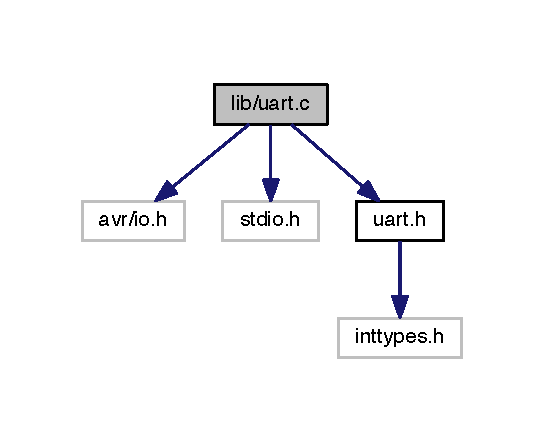
\includegraphics[width=261pt]{uart_8c__incl}
\end{center}
\end{figure}
\subsection*{Macros}
\begin{DoxyCompactItemize}
\item 
\#define \hyperlink{uart_8c_a4af1f98739205bc7f532b0a93e899867}{U\-S\-E\-\_\-\-U2\-X}~1
\item 
\#define \hyperlink{uart_8c_aa5be9eab1b4ef100a79c12228668f5a9}{R\-X\-\_\-\-B\-U\-F\-S\-I\-Z\-E}~80
\end{DoxyCompactItemize}
\subsection*{Functions}
\begin{DoxyCompactItemize}
\item 
uint8\-\_\-t \hyperlink{uart_8c_a8a42498d12d934e63b9b071228a7f39b}{U\-A\-R\-T\-\_\-char\-\_\-received} (void)
\item 
void \hyperlink{uart_8c_ad36599f57b7f2fe3d1d9ee67b937dfdb}{U\-A\-R\-T\-\_\-clr\-\_\-rx\-\_\-buf} (void)
\item 
void \hyperlink{uart_8c_a821ba6a21f4896a9a815940bfcf5d45c}{U\-A\-R\-T\-\_\-init} (uint32\-\_\-t baudrate)
\begin{DoxyCompactList}\small\item\em Initialisierung einer seriellen Konsole. \end{DoxyCompactList}\end{DoxyCompactItemize}
\subsection*{Variables}
\begin{DoxyCompactItemize}
\item 
\hyperlink{uart_8c_a6648dcc0020e15c092b02dd12e434e58}{A\-R\-C\-H\-I\-T\-E\-C\-T\-U\-R\-E\-\_\-undefined} = Hier\-\_\-ist\-\_\-ein\-\_\-\-Fehler
\item 
\hyperlink{uart_8c_a36168cb1b389d05ce98996622774e52d}{F\-\_\-\-C\-P\-U\-\_\-nicht\-\_\-definiert} = Hier\-\_\-ist\-\_\-ein\-\_\-\-Fehler
\end{DoxyCompactItemize}


\subsection{Macro Definition Documentation}
\hypertarget{uart_8c_aa5be9eab1b4ef100a79c12228668f5a9}{\index{uart.\-c@{uart.\-c}!R\-X\-\_\-\-B\-U\-F\-S\-I\-Z\-E@{R\-X\-\_\-\-B\-U\-F\-S\-I\-Z\-E}}
\index{R\-X\-\_\-\-B\-U\-F\-S\-I\-Z\-E@{R\-X\-\_\-\-B\-U\-F\-S\-I\-Z\-E}!uart.c@{uart.\-c}}
\subsubsection[{R\-X\-\_\-\-B\-U\-F\-S\-I\-Z\-E}]{\setlength{\rightskip}{0pt plus 5cm}\#define R\-X\-\_\-\-B\-U\-F\-S\-I\-Z\-E~80}}\label{uart_8c_aa5be9eab1b4ef100a79c12228668f5a9}


Definition at line 97 of file uart.\-c.

\hypertarget{uart_8c_a4af1f98739205bc7f532b0a93e899867}{\index{uart.\-c@{uart.\-c}!U\-S\-E\-\_\-\-U2\-X@{U\-S\-E\-\_\-\-U2\-X}}
\index{U\-S\-E\-\_\-\-U2\-X@{U\-S\-E\-\_\-\-U2\-X}!uart.c@{uart.\-c}}
\subsubsection[{U\-S\-E\-\_\-\-U2\-X}]{\setlength{\rightskip}{0pt plus 5cm}\#define U\-S\-E\-\_\-\-U2\-X~1}}\label{uart_8c_a4af1f98739205bc7f532b0a93e899867}


Definition at line 96 of file uart.\-c.



\subsection{Function Documentation}
\hypertarget{uart_8c_a8a42498d12d934e63b9b071228a7f39b}{\index{uart.\-c@{uart.\-c}!U\-A\-R\-T\-\_\-char\-\_\-received@{U\-A\-R\-T\-\_\-char\-\_\-received}}
\index{U\-A\-R\-T\-\_\-char\-\_\-received@{U\-A\-R\-T\-\_\-char\-\_\-received}!uart.c@{uart.\-c}}
\subsubsection[{U\-A\-R\-T\-\_\-char\-\_\-received}]{\setlength{\rightskip}{0pt plus 5cm}uint8\-\_\-t U\-A\-R\-T\-\_\-char\-\_\-received (
\begin{DoxyParamCaption}
\item[{void}]{}
\end{DoxyParamCaption}
)}}\label{uart_8c_a8a42498d12d934e63b9b071228a7f39b}


Definition at line 112 of file uart.\-c.

\hypertarget{uart_8c_ad36599f57b7f2fe3d1d9ee67b937dfdb}{\index{uart.\-c@{uart.\-c}!U\-A\-R\-T\-\_\-clr\-\_\-rx\-\_\-buf@{U\-A\-R\-T\-\_\-clr\-\_\-rx\-\_\-buf}}
\index{U\-A\-R\-T\-\_\-clr\-\_\-rx\-\_\-buf@{U\-A\-R\-T\-\_\-clr\-\_\-rx\-\_\-buf}!uart.c@{uart.\-c}}
\subsubsection[{U\-A\-R\-T\-\_\-clr\-\_\-rx\-\_\-buf}]{\setlength{\rightskip}{0pt plus 5cm}void U\-A\-R\-T\-\_\-clr\-\_\-rx\-\_\-buf (
\begin{DoxyParamCaption}
\item[{void}]{}
\end{DoxyParamCaption}
)}}\label{uart_8c_ad36599f57b7f2fe3d1d9ee67b937dfdb}


Definition at line 118 of file uart.\-c.

\hypertarget{uart_8c_a821ba6a21f4896a9a815940bfcf5d45c}{\index{uart.\-c@{uart.\-c}!U\-A\-R\-T\-\_\-init@{U\-A\-R\-T\-\_\-init}}
\index{U\-A\-R\-T\-\_\-init@{U\-A\-R\-T\-\_\-init}!uart.c@{uart.\-c}}
\subsubsection[{U\-A\-R\-T\-\_\-init}]{\setlength{\rightskip}{0pt plus 5cm}void U\-A\-R\-T\-\_\-init (
\begin{DoxyParamCaption}
\item[{uint32\-\_\-t}]{baudrate}
\end{DoxyParamCaption}
)}}\label{uart_8c_a821ba6a21f4896a9a815940bfcf5d45c}


Initialisierung einer seriellen Konsole. 


\begin{DoxyParams}{Parameters}
{\em baudrate} & Gew�nschte Baudrate der seriellen Konsole.\\
\hline
\end{DoxyParams}
Um die serielle Schnittstelle einzurichten, muss diese Funktion aufgerufen werden. F�r den Parameter {\itshape baudrate} sollten gebr�uchliche Werte wie 9600, 19200 und, je nach Kabell�nge, auch 115200 verwendet werden. Hierbei ist das U\-S\-A\-R\-T-\/\-Kapitel, insbesondere die am Kapitelende aufgef�hrten Daten der Tabelle "Examples of U\-B\-R\-R Settings for Commonly Used Oscillator Frequencies" der Herstellerdokumentation des Mikrocontrollers zu beachten, nach dem sich nicht f�r jede Oszillatorfrequenz g�ltige Toleranzwerte f�r alle �bertragungsraten ergeben werden. 

Definition at line 128 of file uart.\-c.



\subsection{Variable Documentation}
\hypertarget{uart_8c_a6648dcc0020e15c092b02dd12e434e58}{\index{uart.\-c@{uart.\-c}!A\-R\-C\-H\-I\-T\-E\-C\-T\-U\-R\-E\-\_\-undefined@{A\-R\-C\-H\-I\-T\-E\-C\-T\-U\-R\-E\-\_\-undefined}}
\index{A\-R\-C\-H\-I\-T\-E\-C\-T\-U\-R\-E\-\_\-undefined@{A\-R\-C\-H\-I\-T\-E\-C\-T\-U\-R\-E\-\_\-undefined}!uart.c@{uart.\-c}}
\subsubsection[{A\-R\-C\-H\-I\-T\-E\-C\-T\-U\-R\-E\-\_\-undefined}]{\setlength{\rightskip}{0pt plus 5cm}A\-R\-C\-H\-I\-T\-E\-C\-T\-U\-R\-E\-\_\-undefined = Hier\-\_\-ist\-\_\-ein\-\_\-\-Fehler}}\label{uart_8c_a6648dcc0020e15c092b02dd12e434e58}


Definition at line 85 of file uart.\-c.

\hypertarget{uart_8c_a36168cb1b389d05ce98996622774e52d}{\index{uart.\-c@{uart.\-c}!F\-\_\-\-C\-P\-U\-\_\-nicht\-\_\-definiert@{F\-\_\-\-C\-P\-U\-\_\-nicht\-\_\-definiert}}
\index{F\-\_\-\-C\-P\-U\-\_\-nicht\-\_\-definiert@{F\-\_\-\-C\-P\-U\-\_\-nicht\-\_\-definiert}!uart.c@{uart.\-c}}
\subsubsection[{F\-\_\-\-C\-P\-U\-\_\-nicht\-\_\-definiert}]{\setlength{\rightskip}{0pt plus 5cm}F\-\_\-\-C\-P\-U\-\_\-nicht\-\_\-definiert = Hier\-\_\-ist\-\_\-ein\-\_\-\-Fehler}}\label{uart_8c_a36168cb1b389d05ce98996622774e52d}


Definition at line 93 of file uart.\-c.


\hypertarget{uart_8h}{\section{lib/uart.h File Reference}
\label{uart_8h}\index{lib/uart.\-h@{lib/uart.\-h}}
}


Initialisierung einer seriellen Konsole.  


{\ttfamily \#include $<$inttypes.\-h$>$}\\*
Include dependency graph for uart.\-h\-:\nopagebreak
\begin{figure}[H]
\begin{center}
\leavevmode
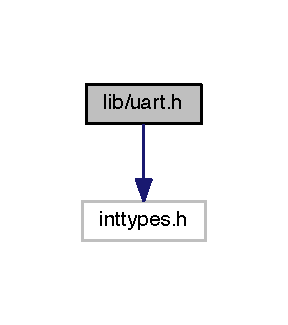
\includegraphics[width=138pt]{uart_8h__incl}
\end{center}
\end{figure}
This graph shows which files directly or indirectly include this file\-:\nopagebreak
\begin{figure}[H]
\begin{center}
\leavevmode
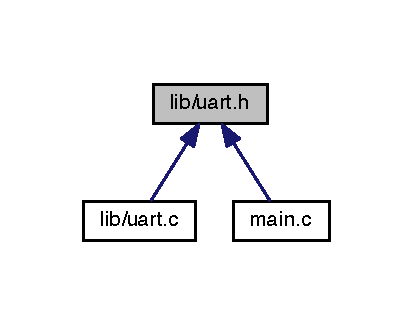
\includegraphics[width=198pt]{uart_8h__dep__incl}
\end{center}
\end{figure}
\subsection*{Functions}
\begin{DoxyCompactItemize}
\item 
uint8\-\_\-t \hyperlink{uart_8h_a8a42498d12d934e63b9b071228a7f39b}{U\-A\-R\-T\-\_\-char\-\_\-received} (void)
\item 
void \hyperlink{uart_8h_ad36599f57b7f2fe3d1d9ee67b937dfdb}{U\-A\-R\-T\-\_\-clr\-\_\-rx\-\_\-buf} (void)
\item 
void \hyperlink{uart_8h_a821ba6a21f4896a9a815940bfcf5d45c}{U\-A\-R\-T\-\_\-init} (uint32\-\_\-t baudrate)
\begin{DoxyCompactList}\small\item\em Initialisierung einer seriellen Konsole. \end{DoxyCompactList}\end{DoxyCompactItemize}


\subsection{Detailed Description}
Initialisierung einer seriellen Konsole. Durch das Modul {\itshape uart} werden die Standard-\/\-Datenstr�me \href{http://de.wikipedia.org/wiki/Stdin}{\tt stdin}, \href{http://de.wikipedia.org/wiki/Stdout}{\tt stdout} und \href{http://de.wikipedia.org/wiki/Stderr}{\tt stderr} mit dem {\itshape U\-S\-A\-R\-T-\/}Ger�t des \href{http://www.atmel.com/}{\tt A\-Tmega32} verbunden. Physikalisch steht diese serielle Schnittstelle nach au�en gem�� dem \href{http://de.wikipedia.org/wiki/EIA-232}{\tt E\-I\-A-\/232-\/}Standard zur Verf�gung und kann somit mit einem P\-C verbunden werden. Standardm��ig wird das System in der Betriebsart {\itshape 8\-N1 ohne Handshake} eingerichtet.

Nach dem Aufruf von \hyperlink{uart_8c_a821ba6a21f4896a9a815940bfcf5d45c}{U\-A\-R\-T\-\_\-init()} stehen zu Ein-\/ und Ausgabezwecken die in der \href{http://de.wikipedia.org/wiki/Header-Datei}{\tt stdio.\-h-\/}Datei definierten Standard-\/\-Ein-\/ und Ausgabefunktionen der \href{http://www.nongnu.org/avr-libc/}{\tt A\-V\-R Libc} zur Verf�gung, also z.\-B. printf, fgets usw. Siehe auch \href{http://de.wikibooks.org/wiki/C-Programmierung:_Einfache_Ein-_und_Ausgabe}{\tt Einf�hrung}.

Zum Verbinden mit einem P\-C wird zudem ein Terminalprogramm, wie z.\-B. \href{http://hp.vector.co.jp/authors/VA002416/teraterm.html}{\tt Tera Term}, \href{http://de.wikipedia.org/wiki/HyperTerminal}{\tt Hyper\-Terminal} oder \href{http://de.wikipedia.org/wiki/Minicom}{\tt Minicom}, ben�tigt. 

Definition in file \hyperlink{uart_8h_source}{uart.\-h}.



\subsection{Function Documentation}
\hypertarget{uart_8h_a8a42498d12d934e63b9b071228a7f39b}{\index{uart.\-h@{uart.\-h}!U\-A\-R\-T\-\_\-char\-\_\-received@{U\-A\-R\-T\-\_\-char\-\_\-received}}
\index{U\-A\-R\-T\-\_\-char\-\_\-received@{U\-A\-R\-T\-\_\-char\-\_\-received}!uart.h@{uart.\-h}}
\subsubsection[{U\-A\-R\-T\-\_\-char\-\_\-received}]{\setlength{\rightskip}{0pt plus 5cm}uint8\-\_\-t U\-A\-R\-T\-\_\-char\-\_\-received (
\begin{DoxyParamCaption}
\item[{void}]{}
\end{DoxyParamCaption}
)}}\label{uart_8h_a8a42498d12d934e63b9b071228a7f39b}


Definition at line 112 of file uart.\-c.

\hypertarget{uart_8h_ad36599f57b7f2fe3d1d9ee67b937dfdb}{\index{uart.\-h@{uart.\-h}!U\-A\-R\-T\-\_\-clr\-\_\-rx\-\_\-buf@{U\-A\-R\-T\-\_\-clr\-\_\-rx\-\_\-buf}}
\index{U\-A\-R\-T\-\_\-clr\-\_\-rx\-\_\-buf@{U\-A\-R\-T\-\_\-clr\-\_\-rx\-\_\-buf}!uart.h@{uart.\-h}}
\subsubsection[{U\-A\-R\-T\-\_\-clr\-\_\-rx\-\_\-buf}]{\setlength{\rightskip}{0pt plus 5cm}void U\-A\-R\-T\-\_\-clr\-\_\-rx\-\_\-buf (
\begin{DoxyParamCaption}
\item[{void}]{}
\end{DoxyParamCaption}
)}}\label{uart_8h_ad36599f57b7f2fe3d1d9ee67b937dfdb}


Definition at line 118 of file uart.\-c.

\hypertarget{uart_8h_a821ba6a21f4896a9a815940bfcf5d45c}{\index{uart.\-h@{uart.\-h}!U\-A\-R\-T\-\_\-init@{U\-A\-R\-T\-\_\-init}}
\index{U\-A\-R\-T\-\_\-init@{U\-A\-R\-T\-\_\-init}!uart.h@{uart.\-h}}
\subsubsection[{U\-A\-R\-T\-\_\-init}]{\setlength{\rightskip}{0pt plus 5cm}void U\-A\-R\-T\-\_\-init (
\begin{DoxyParamCaption}
\item[{uint32\-\_\-t}]{baudrate}
\end{DoxyParamCaption}
)}}\label{uart_8h_a821ba6a21f4896a9a815940bfcf5d45c}


Initialisierung einer seriellen Konsole. 


\begin{DoxyParams}{Parameters}
{\em baudrate} & Gew�nschte Baudrate der seriellen Konsole.\\
\hline
\end{DoxyParams}
Um die serielle Schnittstelle einzurichten, muss diese Funktion aufgerufen werden. F�r den Parameter {\itshape baudrate} sollten gebr�uchliche Werte wie 9600, 19200 und, je nach Kabell�nge, auch 115200 verwendet werden. Hierbei ist das U\-S\-A\-R\-T-\/\-Kapitel, insbesondere die am Kapitelende aufgef�hrten Daten der Tabelle "Examples of U\-B\-R\-R Settings for Commonly Used Oscillator Frequencies" der Herstellerdokumentation des Mikrocontrollers zu beachten, nach dem sich nicht f�r jede Oszillatorfrequenz g�ltige Toleranzwerte f�r alle �bertragungsraten ergeben werden. 

Definition at line 128 of file uart.\-c.


\hypertarget{main_8c}{\section{main.\-c File Reference}
\label{main_8c}\index{main.\-c@{main.\-c}}
}
{\ttfamily \#include \char`\"{}main.\-h\char`\"{}}\\*
{\ttfamily \#include $<$avr/io.\-h$>$}\\*
{\ttfamily \#include $<$util/delay.\-h$>$}\\*
{\ttfamily \#include $<$stdio.\-h$>$}\\*
{\ttfamily \#include $<$stdbool.\-h$>$}\\*
{\ttfamily \#include \char`\"{}lib/uart.\-h\char`\"{}}\\*
{\ttfamily \#include \char`\"{}lib/twi\-\_\-master.\-h\char`\"{}}\\*
{\ttfamily \#include \char`\"{}acceleration\-\_\-t.\-h\char`\"{}}\\*
{\ttfamily \#include \char`\"{}bma020.\-h\char`\"{}}\\*
Include dependency graph for main.\-c\-:
\nopagebreak
\begin{figure}[H]
\begin{center}
\leavevmode
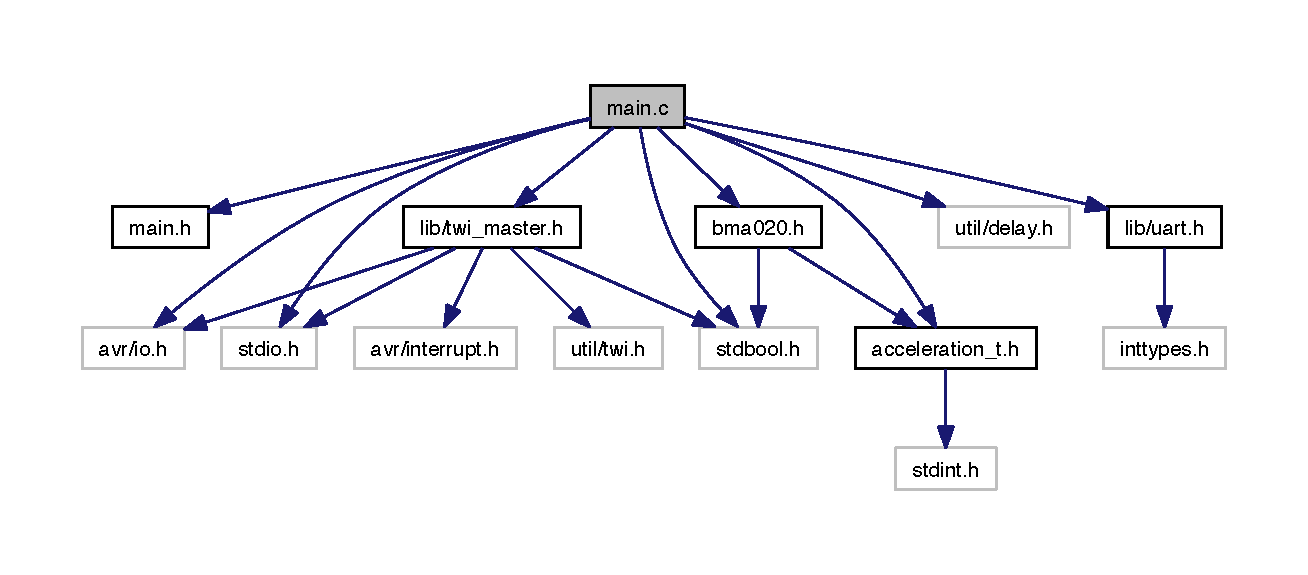
\includegraphics[width=350pt]{main_8c__incl}
\end{center}
\end{figure}
\subsection*{Functions}
\begin{DoxyCompactItemize}
\item 
int \hyperlink{main_8c_a840291bc02cba5474a4cb46a9b9566fe}{main} (void)
\end{DoxyCompactItemize}


\subsection{Function Documentation}
\hypertarget{main_8c_a840291bc02cba5474a4cb46a9b9566fe}{\index{main.\-c@{main.\-c}!main@{main}}
\index{main@{main}!main.c@{main.\-c}}
\subsubsection[{main}]{\setlength{\rightskip}{0pt plus 5cm}int main (
\begin{DoxyParamCaption}
\item[{void}]{}
\end{DoxyParamCaption}
)}}\label{main_8c_a840291bc02cba5474a4cb46a9b9566fe}
Does something important \begin{DoxyReturn}{Returns}

\end{DoxyReturn}


Definition at line 210 of file main.\-c.


\hypertarget{main_8h}{\section{main.\-h File Reference}
\label{main_8h}\index{main.\-h@{main.\-h}}
}
This graph shows which files directly or indirectly include this file\-:\nopagebreak
\begin{figure}[H]
\begin{center}
\leavevmode
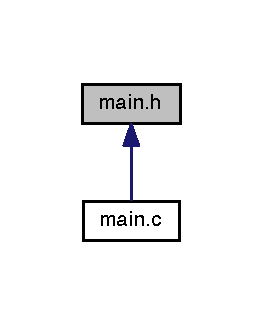
\includegraphics[width=126pt]{main_8h__dep__incl}
\end{center}
\end{figure}
\subsection*{Functions}
\begin{DoxyCompactItemize}
\item 
int \hyperlink{main_8h_a840291bc02cba5474a4cb46a9b9566fe}{main} (void)
\end{DoxyCompactItemize}


\subsection{Function Documentation}
\hypertarget{main_8h_a840291bc02cba5474a4cb46a9b9566fe}{\index{main.\-h@{main.\-h}!main@{main}}
\index{main@{main}!main.h@{main.\-h}}
\subsubsection[{main}]{\setlength{\rightskip}{0pt plus 5cm}int main (
\begin{DoxyParamCaption}
\item[{void}]{}
\end{DoxyParamCaption}
)}}\label{main_8h_a840291bc02cba5474a4cb46a9b9566fe}
Does something important \begin{DoxyReturn}{Returns}

\end{DoxyReturn}


Definition at line 210 of file main.\-c.


%--- End generated contents ---

% Index
\newpage
\phantomsection
\addcontentsline{toc}{part}{Index}
\printindex

\end{document}
